\documentclass[twoside]{book}

% Packages required by doxygen
\usepackage{fixltx2e}
\usepackage{calc}
\usepackage{doxygen}
\usepackage{graphicx}
\usepackage[utf8]{inputenc}
\usepackage{makeidx}
\usepackage{multicol}
\usepackage{multirow}
\PassOptionsToPackage{warn}{textcomp}
\usepackage{textcomp}
\usepackage[nointegrals]{wasysym}
\usepackage[table]{xcolor}

% Font selection
\usepackage[T1]{fontenc}
\usepackage{mathptmx}
\usepackage[scaled=.90]{helvet}
\usepackage{courier}
\usepackage{amssymb}
\usepackage{sectsty}
\renewcommand{\familydefault}{\sfdefault}
\allsectionsfont{%
  \fontseries{bc}\selectfont%
  \color{darkgray}%
}
\renewcommand{\DoxyLabelFont}{%
  \fontseries{bc}\selectfont%
  \color{darkgray}%
}
\newcommand{\+}{\discretionary{\mbox{\scriptsize$\hookleftarrow$}}{}{}}

% Page & text layout
\usepackage{geometry}
\geometry{%
  a4paper,%
  top=2.5cm,%
  bottom=2.5cm,%
  left=2.5cm,%
  right=2.5cm%
}
\tolerance=750
\hfuzz=15pt
\hbadness=750
\setlength{\emergencystretch}{15pt}
\setlength{\parindent}{0cm}
\setlength{\parskip}{0.2cm}
\makeatletter
\renewcommand{\paragraph}{%
  \@startsection{paragraph}{4}{0ex}{-1.0ex}{1.0ex}{%
    \normalfont\normalsize\bfseries\SS@parafont%
  }%
}
\renewcommand{\subparagraph}{%
  \@startsection{subparagraph}{5}{0ex}{-1.0ex}{1.0ex}{%
    \normalfont\normalsize\bfseries\SS@subparafont%
  }%
}
\makeatother

% Headers & footers
\usepackage{fancyhdr}
\pagestyle{fancyplain}
\fancyhead[LE]{\fancyplain{}{\bfseries\thepage}}
\fancyhead[CE]{\fancyplain{}{}}
\fancyhead[RE]{\fancyplain{}{\bfseries\leftmark}}
\fancyhead[LO]{\fancyplain{}{\bfseries\rightmark}}
\fancyhead[CO]{\fancyplain{}{}}
\fancyhead[RO]{\fancyplain{}{\bfseries\thepage}}
\fancyfoot[LE]{\fancyplain{}{}}
\fancyfoot[CE]{\fancyplain{}{}}
\fancyfoot[RE]{\fancyplain{}{\bfseries\scriptsize Generated on Thu Feb 5 2015 15\+:17\+:26 for Fact\+Dev by Doxygen }}
\fancyfoot[LO]{\fancyplain{}{\bfseries\scriptsize Generated on Thu Feb 5 2015 15\+:17\+:26 for Fact\+Dev by Doxygen }}
\fancyfoot[CO]{\fancyplain{}{}}
\fancyfoot[RO]{\fancyplain{}{}}
\renewcommand{\footrulewidth}{0.4pt}
\renewcommand{\chaptermark}[1]{%
  \markboth{#1}{}%
}
\renewcommand{\sectionmark}[1]{%
  \markright{\thesection\ #1}%
}

% Indices & bibliography
\usepackage{natbib}
\usepackage[titles]{tocloft}
\setcounter{tocdepth}{3}
\setcounter{secnumdepth}{5}
\makeindex

% Hyperlinks (required, but should be loaded last)
\usepackage{ifpdf}
\ifpdf
  \usepackage[pdftex,pagebackref=true]{hyperref}
\else
  \usepackage[ps2pdf,pagebackref=true]{hyperref}
\fi
\hypersetup{%
  colorlinks=true,%
  linkcolor=blue,%
  citecolor=blue,%
  unicode%
}

% Custom commands
\newcommand{\clearemptydoublepage}{%
  \newpage{\pagestyle{empty}\cleardoublepage}%
}


%===== C O N T E N T S =====

\begin{document}

% Titlepage & ToC
\hypersetup{pageanchor=false,
             bookmarks=true,
             bookmarksnumbered=true,
             pdfencoding=unicode
            }
\pagenumbering{roman}
\begin{titlepage}
\vspace*{7cm}
\begin{center}%
{\Large Fact\+Dev \\[1ex]\large 0.\+1 }\\
\vspace*{1cm}
{\large Generated by Doxygen 1.8.8}\\
\vspace*{0.5cm}
{\small Thu Feb 5 2015 15:17:26}\\
\end{center}
\end{titlepage}
\clearemptydoublepage
\tableofcontents
\clearemptydoublepage
\pagenumbering{arabic}
\hypersetup{pageanchor=true}

%--- Begin generated contents ---
\chapter{Fact\+Dev documentation}
\label{index}\hypertarget{index}{}This website contains the documentation of Fact\+Dev, a billings and quotes software.

\section*{Team}

F\+A\+C\+T team is a team for Universitiy Project. Members of this team are \+:
\begin{DoxyItemize}
\item Florent Berbie (\href{https://github.com/KraTuX31 KraTuX31}{\tt Kra\+Tu\+X31})
\item Antoine de Roquemaurel (\href{https://github.com/aroquemaurel}{\tt aroquemaurel})
\item Cédric Rohaut (\href{https://github.com/Oxynos}{\tt Oxynos})
\item Manantsoa Andriamihary Razanajatovo (\href{https://github.com/manantsoa}{\tt manantsoa})
\end{DoxyItemize}

For more informations, you can go to \href{http://fact-team.github.io}{\tt http\+://fact-\/team.\+github.\+io}.

\section*{What is Fact\+Dev ?}

 

Fact\+Dev is a software for quotes and billings developped by F\+A\+C\+T team for university project in Toulouse I\+I\+I University – Paul Sabatier.

This software is developped with C++ and Qt framework, and there is differents features \+:
\begin{DoxyItemize}
\item Customers database
\item Differents projects for customers
\item Quotes
\item Billings
\end{DoxyItemize}

\section*{Documentation}

You can access to the documentation generated by Doxygen here \+:
\begin{DoxyItemize}
\item \href{http://fact-team.github.io/doc/html/index.html}{\tt H\+T\+M\+L Documentation}
\item \href{http://fact-team.github.io/doc/latex/refman.pdf}{\tt P\+D\+F Documentation}
\end{DoxyItemize}

\section*{Installation and using}


\begin{DoxyItemize}
\item \href{http://fact-team.github.io/doc/usermanual.pdf}{\tt User Manual} 
\end{DoxyItemize}
\chapter{Q\+Test\+Runner}
\label{dc/d04/md_tests_QTestRunner_README}
\hypertarget{dc/d04/md_tests_QTestRunner_README}{}
A repo for Increase Q\+Test productivity

Thanks to \href{https://marcoarena.wordpress.com/2012/06/23/increase-your-qtest-productivity/}{\tt https\+://marcoarena.\+wordpress.\+com/2012/06/23/increase-\/your-\/qtest-\/productivity/} ! \begin{quote}
The Q\+Test\+Lib framework is a tool for unit testing Qt based applications and libraries. I find it precious and simple to use, though it lacks some important features, supported, for example, by G\+Test. I’m not talking about mocking – for this you generally need an out-\/and-\/out framework (like G\+Mock) – instead, I’m referring to simple things like fast deploying. Suppose you have written a test class like this\+: \end{quote}


This repo contains only the code in this article. 
\chapter{Namespace Index}
\section{Namespace List}
Here is a list of all documented namespaces with brief descriptions\-:\begin{DoxyCompactList}
\item\contentsline{section}{\hyperlink{namespaceDatabases}{Databases} \\*Class for \hyperlink{classDatabases_1_1Database}{Database}, contains queries }{\pageref{df/d31/namespaceDatabases}}{}
\item\contentsline{section}{\hyperlink{namespaceGui}{Gui} }{\pageref{d9/dad/namespaceGui}}{}
\item\contentsline{section}{\hyperlink{namespaceGui_1_1Widgets}{Gui\-::\-Widgets} \\*Contains \hyperlink{namespaceGui_1_1Widgets}{Widgets} classes }{\pageref{d4/dfe/namespaceGui_1_1Widgets}}{}
\item\contentsline{section}{\hyperlink{namespaceModels}{Models} \\*\hyperlink{namespaceModels}{Models} classes }{\pageref{dd/d20/namespaceModels}}{}
\end{DoxyCompactList}

\chapter{Hierarchical Index}
\section{Class Hierarchy}
This inheritance list is sorted roughly, but not completely, alphabetically\-:\begin{DoxyCompactList}
\item \contentsline{section}{Mustache\-:\-:Context}{\pageref{d7/d34/classMustache_1_1Context}}{}
\begin{DoxyCompactList}
\item \contentsline{section}{Mustache\-:\-:Qt\-Variant\-Context}{\pageref{d5/d8b/classMustache_1_1QtVariantContext}}{}
\begin{DoxyCompactList}
\item \contentsline{section}{Counter\-Context}{\pageref{db/da6/classCounterContext}}{}
\item \contentsline{section}{Counter\-Context}{\pageref{db/da6/classCounterContext}}{}
\end{DoxyCompactList}
\end{DoxyCompactList}
\item \contentsline{section}{Contributory\-List\-Test}{\pageref{d4/de2/classContributoryListTest}}{}
\item \contentsline{section}{Databases\-:\-:Database}{\pageref{dd/db0/classDatabases_1_1Database}}{}
\begin{DoxyCompactList}
\item \contentsline{section}{Databases\-:\-:Billing\-Database}{\pageref{df/df8/classDatabases_1_1BillingDatabase}}{}
\item \contentsline{section}{Databases\-:\-:Contributory\-Database}{\pageref{dc/da5/classDatabases_1_1ContributoryDatabase}}{}
\item \contentsline{section}{Databases\-:\-:Customer\-Database}{\pageref{d8/d7e/classDatabases_1_1CustomerDatabase}}{}
\item \contentsline{section}{Databases\-:\-:Project\-Database}{\pageref{d7/d39/classDatabases_1_1ProjectDatabase}}{}
\item \contentsline{section}{Databases\-:\-:Rate\-Database}{\pageref{d9/d21/classDatabases_1_1RateDatabase}}{}
\item \contentsline{section}{Databases\-:\-:User\-Database}{\pageref{d0/d33/classDatabases_1_1UserDatabase}}{}
\end{DoxyCompactList}
\item \contentsline{section}{Utils\-:\-:Directories}{\pageref{d8/d40/classUtils_1_1Directories}}{}
\item exception\begin{DoxyCompactList}
\item \contentsline{section}{Exceptions\-:\-:Db\-Exception}{\pageref{d4/de4/classExceptions_1_1DbException}}{}
\end{DoxyCompactList}
\item \contentsline{section}{Exceptions\-:\-:File\-Exception}{\pageref{d9/d57/classExceptions_1_1FileException}}{}
\item \contentsline{section}{Generator}{\pageref{d9/d12/classGenerator}}{}
\item \contentsline{section}{Utils\-:\-:Hierarchical\-System}{\pageref{d1/de0/classUtils_1_1HierarchicalSystem}}{}
\item \contentsline{section}{Gui\-:\-:Widgets\-:\-:Check\-Fields\-:\-:I\-Check\-Field}{\pageref{d7/d93/classGui_1_1Widgets_1_1CheckFields_1_1ICheckField}}{}
\begin{DoxyCompactList}
\item \contentsline{section}{Gui\-:\-:Widgets\-:\-:Check\-Fields\-:\-:Check\-Q\-Line\-Edit}{\pageref{d0/d68/classGui_1_1Widgets_1_1CheckFields_1_1CheckQLineEdit}}{}
\begin{DoxyCompactList}
\item \contentsline{section}{Gui\-:\-:Widgets\-:\-:Check\-Fields\-:\-:Check\-Email}{\pageref{d1/d07/classGui_1_1Widgets_1_1CheckFields_1_1CheckEmail}}{}
\item \contentsline{section}{Gui\-:\-:Widgets\-:\-:Check\-Fields\-:\-:Check\-Siret\-Number}{\pageref{db/d94/classGui_1_1Widgets_1_1CheckFields_1_1CheckSiretNumber}}{}
\item \contentsline{section}{Gui\-:\-:Widgets\-:\-:Check\-Fields\-:\-:Check\-Until\-Field}{\pageref{d4/d37/classGui_1_1Widgets_1_1CheckFields_1_1CheckUntilField}}{}
\begin{DoxyCompactList}
\item \contentsline{section}{Gui\-:\-:Widgets\-:\-:Check\-Fields\-:\-:Check\-Fields\-Letters}{\pageref{df/dba/classGui_1_1Widgets_1_1CheckFields_1_1CheckFieldsLetters}}{}
\begin{DoxyCompactList}
\item \contentsline{section}{Gui\-:\-:Widgets\-:\-:Check\-Fields\-:\-:Check\-City}{\pageref{dd/da5/classGui_1_1Widgets_1_1CheckFields_1_1CheckCity}}{}
\item \contentsline{section}{Gui\-:\-:Widgets\-:\-:Check\-Fields\-:\-:Check\-Country}{\pageref{d0/d3f/classGui_1_1Widgets_1_1CheckFields_1_1CheckCountry}}{}
\item \contentsline{section}{Gui\-:\-:Widgets\-:\-:Check\-Fields\-:\-:Check\-Name}{\pageref{da/d67/classGui_1_1Widgets_1_1CheckFields_1_1CheckName}}{}
\end{DoxyCompactList}
\item \contentsline{section}{Gui\-:\-:Widgets\-:\-:Check\-Fields\-:\-:Check\-Phone}{\pageref{da/dc0/classGui_1_1Widgets_1_1CheckFields_1_1CheckPhone}}{}
\item \contentsline{section}{Gui\-:\-:Widgets\-:\-:Check\-Fields\-:\-:Check\-Postal\-Code}{\pageref{df/d31/classGui_1_1Widgets_1_1CheckFields_1_1CheckPostalCode}}{}
\end{DoxyCompactList}
\item \contentsline{section}{Gui\-:\-:Widgets\-:\-:Check\-Fields\-:\-:Check\-Valid\-Field}{\pageref{d8/d6d/classGui_1_1Widgets_1_1CheckFields_1_1CheckValidField}}{}
\end{DoxyCompactList}
\end{DoxyCompactList}
\item \contentsline{section}{Models\-:\-:I\-Model}{\pageref{d0/d9c/classModels_1_1IModel}}{}
\begin{DoxyCompactList}
\item \contentsline{section}{Models\-:\-:Billing}{\pageref{d4/d5c/classModels_1_1Billing}}{}
\item \contentsline{section}{Models\-:\-:Contributory}{\pageref{d5/dd1/classModels_1_1Contributory}}{}
\item \contentsline{section}{Models\-:\-:Customer}{\pageref{db/dd7/classModels_1_1Customer}}{}
\item \contentsline{section}{Models\-:\-:Project}{\pageref{dd/d3f/classModels_1_1Project}}{}
\item \contentsline{section}{Models\-:\-:User}{\pageref{df/d68/classModels_1_1User}}{}
\end{DoxyCompactList}
\item \contentsline{section}{Utils\-:\-:Item\-Type}{\pageref{d5/d7c/classUtils_1_1ItemType}}{}
\item \contentsline{section}{Utils\-:\-:Log}{\pageref{db/db3/classUtils_1_1Log}}{}
\item \contentsline{section}{Parameters}{\pageref{de/d0a/classParameters}}{}
\item \contentsline{section}{Mustache\-:\-:Partial\-Resolver}{\pageref{d0/dce/classMustache_1_1PartialResolver}}{}
\begin{DoxyCompactList}
\item \contentsline{section}{Mustache\-:\-:Partial\-File\-Loader}{\pageref{da/d31/classMustache_1_1PartialFileLoader}}{}
\item \contentsline{section}{Mustache\-:\-:Partial\-Map}{\pageref{dc/d1a/classMustache_1_1PartialMap}}{}
\end{DoxyCompactList}
\item \contentsline{section}{Utils\-:\-:pointers}{\pageref{d4/d7a/classUtils_1_1pointers}}{}
\item \contentsline{section}{Gui\-:\-:Widgets\-:\-:Popup}{\pageref{d4/d2f/classGui_1_1Widgets_1_1Popup}}{}
\item Q\-Abstract\-Table\-Model\begin{DoxyCompactList}
\item \contentsline{section}{Gui\-:\-:Widgets\-:\-:Wdg\-Models\-:\-:Billings\-Table\-Model}{\pageref{dc/d82/classGui_1_1Widgets_1_1WdgModels_1_1BillingsTableModel}}{}
\item \contentsline{section}{Gui\-:\-:Widgets\-:\-:Wdg\-Models\-:\-:Contributories\-Table\-Model}{\pageref{dc/db9/classGui_1_1Widgets_1_1WdgModels_1_1ContributoriesTableModel}}{}
\item \contentsline{section}{Gui\-:\-:Widgets\-:\-:Wdg\-Models\-:\-:Customers\-Table\-Model}{\pageref{d7/d12/classGui_1_1Widgets_1_1WdgModels_1_1CustomersTableModel}}{}
\item \contentsline{section}{Gui\-:\-:Widgets\-:\-:Wdg\-Models\-:\-:Project\-Contributories\-Table\-Model}{\pageref{d9/d71/classGui_1_1Widgets_1_1WdgModels_1_1ProjectContributoriesTableModel}}{}
\item \contentsline{section}{Gui\-:\-:Widgets\-:\-:Wdg\-Models\-:\-:Projects\-Table\-Model}{\pageref{d3/d40/classGui_1_1Widgets_1_1WdgModels_1_1ProjectsTableModel}}{}
\end{DoxyCompactList}
\item Q\-Dialog\begin{DoxyCompactList}
\item \contentsline{section}{Gui\-:\-:Dialogs\-:\-:Add\-Project\-Dialog}{\pageref{de/d36/classGui_1_1Dialogs_1_1AddProjectDialog}}{}
\item \contentsline{section}{Gui\-:\-:Dialogs\-:\-:Add\-Quote\-Dialog}{\pageref{d6/d43/classGui_1_1Dialogs_1_1AddQuoteDialog}}{}
\item \contentsline{section}{Gui\-:\-:Dialogs\-:\-:Dialog\-Add\-Customer}{\pageref{d2/d50/classGui_1_1Dialogs_1_1DialogAddCustomer}}{}
\item \contentsline{section}{Gui\-:\-:Dialogs\-:\-:Message\-Box}{\pageref{d9/d31/classGui_1_1Dialogs_1_1MessageBox}}{}
\item \contentsline{section}{Gui\-:\-:Dialogs\-:\-:User\-Data\-Dialog}{\pageref{d3/d81/classGui_1_1Dialogs_1_1UserDataDialog}}{}
\item \contentsline{section}{Started\-Windows\-Dialog}{\pageref{da/ddc/classStartedWindowsDialog}}{}
\end{DoxyCompactList}
\item Q\-Dock\-Widget\begin{DoxyCompactList}
\item \contentsline{section}{Gui\-:\-:Docks\-:\-:Search\-Dock}{\pageref{de/db4/classGui_1_1Docks_1_1SearchDock}}{}
\end{DoxyCompactList}
\item Q\-Item\-Delegate\begin{DoxyCompactList}
\item \contentsline{section}{Gui\-:\-:Widgets\-:\-:Delegates\-:\-:Combo\-Box\-Delegate}{\pageref{d5/d72/classGui_1_1Widgets_1_1Delegates_1_1ComboBoxDelegate}}{}
\begin{DoxyCompactList}
\item \contentsline{section}{Gui\-:\-:Widgets\-:\-:Delegates\-:\-:Project\-Combo\-Delegate}{\pageref{d6/d93/classGui_1_1Widgets_1_1Delegates_1_1ProjectComboDelegate}}{}
\item \contentsline{section}{Gui\-:\-:Widgets\-:\-:Delegates\-:\-:Unit\-Combo\-Delegate}{\pageref{db/def/classGui_1_1Widgets_1_1Delegates_1_1UnitComboDelegate}}{}
\end{DoxyCompactList}
\item \contentsline{section}{Gui\-:\-:Widgets\-:\-:Delegates\-:\-:Double\-Spin\-Box\-Delegate}{\pageref{da/d53/classGui_1_1Widgets_1_1Delegates_1_1DoubleSpinBoxDelegate}}{}
\end{DoxyCompactList}
\item Q\-Line\-Edit\begin{DoxyCompactList}
\item \contentsline{section}{Gui\-:\-:Widgets\-:\-:Check\-Fields\-:\-:Check\-Q\-Line\-Edit}{\pageref{d0/d68/classGui_1_1Widgets_1_1CheckFields_1_1CheckQLineEdit}}{}
\end{DoxyCompactList}
\item Q\-Main\-Window\begin{DoxyCompactList}
\item \contentsline{section}{Gui\-:\-:Main\-Window}{\pageref{d5/d2f/classGui_1_1MainWindow}}{}
\end{DoxyCompactList}
\item Q\-Map\begin{DoxyCompactList}
\item \contentsline{section}{Models\-:\-:Contributories\-List}{\pageref{d7/d6a/classModels_1_1ContributoriesList}}{}
\end{DoxyCompactList}
\item Q\-Menu\begin{DoxyCompactList}
\item \contentsline{section}{Gui\-:\-:Widgets\-:\-:Customer\-Contextual\-Menu}{\pageref{d8/ded/classGui_1_1Widgets_1_1CustomerContextualMenu}}{}
\end{DoxyCompactList}
\item Q\-Object\begin{DoxyCompactList}
\item \contentsline{section}{Billing\-Database\-Test}{\pageref{d1/db1/classBillingDatabaseTest}}{}
\item \contentsline{section}{Billing\-Model\-Test}{\pageref{dc/d0c/classBillingModelTest}}{}
\item \contentsline{section}{Contributories\-Database\-Test}{\pageref{d8/df7/classContributoriesDatabaseTest}}{}
\item \contentsline{section}{Contributory\-Model\-Test}{\pageref{d5/d97/classContributoryModelTest}}{}
\item \contentsline{section}{Customer\-Database\-Test}{\pageref{d2/d63/classCustomerDatabaseTest}}{}
\item \contentsline{section}{Customer\-Model\-Test}{\pageref{d5/dcd/classCustomerModelTest}}{}
\item \contentsline{section}{Generation}{\pageref{d4/df7/classGeneration}}{}
\item \contentsline{section}{Item\-Type\-Test}{\pageref{d3/de2/classItemTypeTest}}{}
\item \contentsline{section}{Project\-Database\-Test}{\pageref{df/d3e/classProjectDatabaseTest}}{}
\item \contentsline{section}{Project\-Model\-Test}{\pageref{dd/d54/classProjectModelTest}}{}
\item \contentsline{section}{Rate\-Model\-Test}{\pageref{d2/dcd/classRateModelTest}}{}
\item \contentsline{section}{search\-Test}{\pageref{d7/d51/classsearchTest}}{}
\item \contentsline{section}{String\-Test}{\pageref{d1/d6b/classStringTest}}{}
\item \contentsline{section}{Test\-Mustache}{\pageref{de/d63/classTestMustache}}{}
\item \contentsline{section}{Test\-Mustache}{\pageref{de/d63/classTestMustache}}{}
\item \contentsline{section}{User\-Database\-Test}{\pageref{d7/dc1/classUserDatabaseTest}}{}
\item \contentsline{section}{User\-Model\-Test}{\pageref{de/d37/classUserModelTest}}{}
\end{DoxyCompactList}
\item Q\-Widget\begin{DoxyCompactList}
\item \contentsline{section}{Gui\-:\-:Widgets\-:\-:Combo\-Box\-Model\-Widget}{\pageref{d2/de0/classGui_1_1Widgets_1_1ComboBoxModelWidget}}{}
\item \contentsline{section}{Gui\-:\-:Widgets\-:\-:Contributories\-Widget}{\pageref{dc/da3/classGui_1_1Widgets_1_1ContributoriesWidget}}{}
\item \contentsline{section}{Gui\-:\-:Widgets\-:\-:Customer\-Data\-Widget}{\pageref{df/deb/classGui_1_1Widgets_1_1CustomerDataWidget}}{}
\item \contentsline{section}{Gui\-:\-:Widgets\-:\-:Projects\-Widget}{\pageref{dc/d8c/classGui_1_1Widgets_1_1ProjectsWidget}}{}
\item \contentsline{section}{Gui\-:\-:Widgets\-:\-:Rate\-Widget}{\pageref{d0/de2/classGui_1_1Widgets_1_1RateWidget}}{}
\item \contentsline{section}{Gui\-:\-:Widgets\-:\-:search\-Widget}{\pageref{d7/d75/classGui_1_1Widgets_1_1searchWidget}}{}
\end{DoxyCompactList}
\item \contentsline{section}{Models\-:\-:Rate}{\pageref{d9/dc5/classModels_1_1Rate}}{}
\item \contentsline{section}{Mustache\-:\-:Renderer}{\pageref{dc/d58/classMustache_1_1Renderer}}{}
\item \contentsline{section}{Models\-:\-:Search}{\pageref{d6/d44/classModels_1_1Search}}{}
\item \contentsline{section}{Utils\-:\-:String}{\pageref{dd/df6/classUtils_1_1String}}{}
\item \contentsline{section}{Mustache\-:\-:Tag}{\pageref{d5/dc2/structMustache_1_1Tag}}{}
\item \contentsline{section}{Test\-Adder$<$ T $>$}{\pageref{d0/d9b/classTestAdder}}{}
\item \contentsline{section}{testadder}{\pageref{d7/d26/classtestadder}}{}
\item \contentsline{section}{Test\-Runner}{\pageref{db/d70/classTestRunner}}{}
\end{DoxyCompactList}

\chapter{Class Index}
\section{Class List}
Here are the classes, structs, unions and interfaces with brief descriptions\-:\begin{DoxyCompactList}
\item\contentsline{section}{\hyperlink{classDatabases_1_1AccessDatabase}{Databases\-::\-Access\-Database} }{\pageref{d5/dbc/classDatabases_1_1AccessDatabase}}{}
\item\contentsline{section}{\hyperlink{classGui_1_1Dialogs_1_1AddProjectDialog}{Gui\-::\-Dialogs\-::\-Add\-Project\-Dialog} \\*Windows to add a new Project }{\pageref{de/d36/classGui_1_1Dialogs_1_1AddProjectDialog}}{}
\item\contentsline{section}{\hyperlink{classGui_1_1Dialogs_1_1AddQuoteDialog}{Gui\-::\-Dialogs\-::\-Add\-Quote\-Dialog} \\*Window to add or modify a Quote }{\pageref{d6/d43/classGui_1_1Dialogs_1_1AddQuoteDialog}}{}
\item\contentsline{section}{\hyperlink{classModels_1_1Billing}{Models\-::\-Billing} \\*\-: \hyperlink{classModels_1_1Billing}{Billing} or Quote of a \hyperlink{classModels_1_1Customer}{Customer} }{\pageref{d4/d5c/classModels_1_1Billing}}{}
\item\contentsline{section}{\hyperlink{classDatabases_1_1BillingDatabase}{Databases\-::\-Billing\-Database} \\*The {\bfseries \hyperlink{classDatabases_1_1BillingDatabase}{Billing\-Database}} class Billing (or Quote) table database }{\pageref{df/df8/classDatabases_1_1BillingDatabase}}{}
\item\contentsline{section}{\hyperlink{classBillingDatabaseTest}{Billing\-Database\-Test} }{\pageref{d1/db1/classBillingDatabaseTest}}{}
\item\contentsline{section}{\hyperlink{classBillingModelTest}{Billing\-Model\-Test} }{\pageref{dc/d0c/classBillingModelTest}}{}
\item\contentsline{section}{\hyperlink{classGui_1_1Widgets_1_1WdgModels_1_1BillingsTableModel}{Gui\-::\-Widgets\-::\-Wdg\-Models\-::\-Billings\-Table\-Model} \\*For a Billing table }{\pageref{dc/d82/classGui_1_1Widgets_1_1WdgModels_1_1BillingsTableModel}}{}
\item\contentsline{section}{\hyperlink{classModels_1_1Calculable}{Models\-::\-Calculable} \\*The \hyperlink{classModels_1_1Calculable}{Calculable} interface \hyperlink{namespaceModels}{Models} who are calculable }{\pageref{dc/d99/classModels_1_1Calculable}}{}
\item\contentsline{section}{\hyperlink{classGui_1_1Widgets_1_1CheckFields_1_1CheckCity}{Gui\-::\-Widgets\-::\-Check\-Fields\-::\-Check\-City} \\*Line Edit of City with a check icon }{\pageref{dd/da5/classGui_1_1Widgets_1_1CheckFields_1_1CheckCity}}{}
\item\contentsline{section}{\hyperlink{classGui_1_1Widgets_1_1CheckFields_1_1CheckCountry}{Gui\-::\-Widgets\-::\-Check\-Fields\-::\-Check\-Country} \\*\hyperlink{classGui_1_1Widgets_1_1CheckFields_1_1CheckCountry_ae432c47f8bede68b29a89af24b234eef}{Check\-Country\-::\-Check\-Country} Line Edit of country with a check icon }{\pageref{d0/d3f/classGui_1_1Widgets_1_1CheckFields_1_1CheckCountry}}{}
\item\contentsline{section}{\hyperlink{classGui_1_1Widgets_1_1CheckFields_1_1CheckEmail}{Gui\-::\-Widgets\-::\-Check\-Fields\-::\-Check\-Email} \\*Line Edit of email with a check icon }{\pageref{d1/d07/classGui_1_1Widgets_1_1CheckFields_1_1CheckEmail}}{}
\item\contentsline{section}{\hyperlink{classGui_1_1Widgets_1_1CheckFields_1_1CheckFieldsLetters}{Gui\-::\-Widgets\-::\-Check\-Fields\-::\-Check\-Fields\-Letters} \\*Field with only letters (no numbers) }{\pageref{df/dba/classGui_1_1Widgets_1_1CheckFields_1_1CheckFieldsLetters}}{}
\item\contentsline{section}{\hyperlink{classGui_1_1Widgets_1_1CheckFields_1_1CheckFieldsNumbers}{Gui\-::\-Widgets\-::\-Check\-Fields\-::\-Check\-Fields\-Numbers} \\*Line Edit of number with a check icon }{\pageref{d9/daa/classGui_1_1Widgets_1_1CheckFields_1_1CheckFieldsNumbers}}{}
\item\contentsline{section}{\hyperlink{classGui_1_1Widgets_1_1CheckFields_1_1CheckIpAddress}{Gui\-::\-Widgets\-::\-Check\-Fields\-::\-Check\-Ip\-Address} \\*Line Edit of I\-P address with a check icon }{\pageref{db/d70/classGui_1_1Widgets_1_1CheckFields_1_1CheckIpAddress}}{}
\item\contentsline{section}{\hyperlink{classGui_1_1Widgets_1_1CheckFields_1_1CheckLogin}{Gui\-::\-Widgets\-::\-Check\-Fields\-::\-Check\-Login} \\*Line Edit of login with a check icon }{\pageref{dd/dfe/classGui_1_1Widgets_1_1CheckFields_1_1CheckLogin}}{}
\item\contentsline{section}{\hyperlink{classGui_1_1Widgets_1_1CheckFields_1_1CheckName}{Gui\-::\-Widgets\-::\-Check\-Fields\-::\-Check\-Name} \\*Line edit of name with a check icon }{\pageref{da/d67/classGui_1_1Widgets_1_1CheckFields_1_1CheckName}}{}
\item\contentsline{section}{\hyperlink{classGui_1_1Widgets_1_1CheckFields_1_1CheckPhone}{Gui\-::\-Widgets\-::\-Check\-Fields\-::\-Check\-Phone} \\*Line Edit of Phone number with a check icon }{\pageref{da/dc0/classGui_1_1Widgets_1_1CheckFields_1_1CheckPhone}}{}
\item\contentsline{section}{\hyperlink{classGui_1_1Widgets_1_1CheckFields_1_1CheckPortNumber}{Gui\-::\-Widgets\-::\-Check\-Fields\-::\-Check\-Port\-Number} \\*The \hyperlink{classGui_1_1Widgets_1_1CheckFields_1_1CheckFieldsNumbers}{Check\-Fields\-Numbers} class Line Edit of number with a check icon }{\pageref{d5/d41/classGui_1_1Widgets_1_1CheckFields_1_1CheckPortNumber}}{}
\item\contentsline{section}{\hyperlink{classGui_1_1Widgets_1_1CheckFields_1_1CheckPostalCode}{Gui\-::\-Widgets\-::\-Check\-Fields\-::\-Check\-Postal\-Code} \\*Line Edit of postal code with a check icon }{\pageref{df/d31/classGui_1_1Widgets_1_1CheckFields_1_1CheckPostalCode}}{}
\item\contentsline{section}{\hyperlink{classGui_1_1Widgets_1_1CheckFields_1_1CheckQLineEdit}{Gui\-::\-Widgets\-::\-Check\-Fields\-::\-Check\-Q\-Line\-Edit} \\*Line\-Edit custom with a check of text inputed }{\pageref{d0/d68/classGui_1_1Widgets_1_1CheckFields_1_1CheckQLineEdit}}{}
\item\contentsline{section}{\hyperlink{classGui_1_1Widgets_1_1CheckFields_1_1CheckSiretNumber}{Gui\-::\-Widgets\-::\-Check\-Fields\-::\-Check\-Siret\-Number} \\*Line Edit with a check icon }{\pageref{db/d94/classGui_1_1Widgets_1_1CheckFields_1_1CheckSiretNumber}}{}
\item\contentsline{section}{\hyperlink{classGui_1_1Widgets_1_1CheckFields_1_1CheckUntilField}{Gui\-::\-Widgets\-::\-Check\-Fields\-::\-Check\-Until\-Field} \\*The \hyperlink{classGui_1_1Widgets_1_1CheckFields_1_1CheckUntilField}{Check\-Until\-Field} class }{\pageref{d4/d37/classGui_1_1Widgets_1_1CheckFields_1_1CheckUntilField}}{}
\item\contentsline{section}{\hyperlink{classGui_1_1Widgets_1_1CheckFields_1_1CheckValidField}{Gui\-::\-Widgets\-::\-Check\-Fields\-::\-Check\-Valid\-Field} \\*Check field not required }{\pageref{d8/d6d/classGui_1_1Widgets_1_1CheckFields_1_1CheckValidField}}{}
\item\contentsline{section}{\hyperlink{classGui_1_1Widgets_1_1CheckFields_1_1CheckWebsite}{Gui\-::\-Widgets\-::\-Check\-Fields\-::\-Check\-Website} \\*Line Edit of website with a check icon }{\pageref{dd/d1b/classGui_1_1Widgets_1_1CheckFields_1_1CheckWebsite}}{}
\item\contentsline{section}{\hyperlink{classGui_1_1Widgets_1_1Path_1_1ChoseDirectoryWidget}{Gui\-::\-Widgets\-::\-Path\-::\-Chose\-Directory\-Widget} \\*Open a Q\-File\-Dialog.\-and display path in textfield }{\pageref{dd/d67/classGui_1_1Widgets_1_1Path_1_1ChoseDirectoryWidget}}{}
\item\contentsline{section}{\hyperlink{classGui_1_1Widgets_1_1Path_1_1ChoseFileWidget}{Gui\-::\-Widgets\-::\-Path\-::\-Chose\-File\-Widget} \\*Chose a File in computer }{\pageref{da/d61/classGui_1_1Widgets_1_1Path_1_1ChoseFileWidget}}{}
\item\contentsline{section}{\hyperlink{classGui_1_1Widgets_1_1Path_1_1ChosePathWidget}{Gui\-::\-Widgets\-::\-Path\-::\-Chose\-Path\-Widget} \\*The \hyperlink{classGui_1_1Widgets_1_1Path_1_1ChoseDirectoryWidget}{Chose\-Directory\-Widget} class Open a Q\-File\-Dialog.\-and display path in textfield }{\pageref{db/de6/classGui_1_1Widgets_1_1Path_1_1ChosePathWidget}}{}
\item\contentsline{section}{\hyperlink{classGui_1_1Widgets_1_1Delegates_1_1ComboBoxDelegate}{Gui\-::\-Widgets\-::\-Delegates\-::\-Combo\-Box\-Delegate} \\*The \hyperlink{classGui_1_1Widgets_1_1Delegates_1_1ComboBoxDelegate}{Combo\-Box\-Delegate} class }{\pageref{d5/d72/classGui_1_1Widgets_1_1Delegates_1_1ComboBoxDelegate}}{}
\item\contentsline{section}{\hyperlink{classGui_1_1Widgets_1_1ComboBoxModelWidget}{Gui\-::\-Widgets\-::\-Combo\-Box\-Model\-Widget} \\*Model of Combo\-Box }{\pageref{d2/de0/classGui_1_1Widgets_1_1ComboBoxModelWidget}}{}
\item\contentsline{section}{\hyperlink{classGui_1_1Dialogs_1_1ComputeTurnoverDialog}{Gui\-::\-Dialogs\-::\-Compute\-Turnover\-Dialog} \\*Window to compute a turnover with a period }{\pageref{d1/d0e/classGui_1_1Dialogs_1_1ComputeTurnoverDialog}}{}
\item\contentsline{section}{\hyperlink{classMustache_1_1Context}{Mustache\-::\-Context} }{\pageref{d7/d34/classMustache_1_1Context}}{}
\item\contentsline{section}{\hyperlink{classContributoriesDatabaseTest}{Contributories\-Database\-Test} }{\pageref{d8/df7/classContributoriesDatabaseTest}}{}
\item\contentsline{section}{\hyperlink{classModels_1_1ContributoriesList}{Models\-::\-Contributories\-List} \\*List of contributories }{\pageref{d7/d6a/classModels_1_1ContributoriesList}}{}
\item\contentsline{section}{\hyperlink{classGui_1_1Widgets_1_1WdgModels_1_1ContributoriesTableModel}{Gui\-::\-Widgets\-::\-Wdg\-Models\-::\-Contributories\-Table\-Model} \\*For a custom table for contributories widget }{\pageref{dc/db9/classGui_1_1Widgets_1_1WdgModels_1_1ContributoriesTableModel}}{}
\item\contentsline{section}{\hyperlink{classGui_1_1Widgets_1_1ContributoriesWidget}{Gui\-::\-Widgets\-::\-Contributories\-Widget} \\*Widget of Contributories }{\pageref{dc/da3/classGui_1_1Widgets_1_1ContributoriesWidget}}{}
\item\contentsline{section}{\hyperlink{classModels_1_1Contributory}{Models\-::\-Contributory} \\*The \hyperlink{classModels_1_1Unit}{Unit} enum Unity of work \-: hour or day }{\pageref{d5/dd1/classModels_1_1Contributory}}{}
\item\contentsline{section}{\hyperlink{classDatabases_1_1ContributoryDatabase}{Databases\-::\-Contributory\-Database} \\*The {\bfseries \hyperlink{classDatabases_1_1ContributoryDatabase}{Contributory\-Database}} class Contributory (or Quote) table database }{\pageref{dc/da5/classDatabases_1_1ContributoryDatabase}}{}
\item\contentsline{section}{\hyperlink{classContributoryListTest}{Contributory\-List\-Test} }{\pageref{d4/de2/classContributoryListTest}}{}
\item\contentsline{section}{\hyperlink{classContributoryModelTest}{Contributory\-Model\-Test} }{\pageref{d5/d97/classContributoryModelTest}}{}
\item\contentsline{section}{\hyperlink{classCounterContext}{Counter\-Context} }{\pageref{db/da6/classCounterContext}}{}
\item\contentsline{section}{\hyperlink{classModels_1_1Customer}{Models\-::\-Customer} \\*\hyperlink{classModels_1_1Customer}{Customer} }{\pageref{db/dd7/classModels_1_1Customer}}{}
\item\contentsline{section}{\hyperlink{classGui_1_1Widgets_1_1CustomerContextualMenu}{Gui\-::\-Widgets\-::\-Customer\-Contextual\-Menu} \\*Display contextual menu on a customer }{\pageref{d8/ded/classGui_1_1Widgets_1_1CustomerContextualMenu}}{}
\item\contentsline{section}{\hyperlink{classDatabases_1_1CustomerDatabase}{Databases\-::\-Customer\-Database} \\*The {\bfseries \hyperlink{classDatabases_1_1CustomerDatabase}{Customer\-Database}} class Customer table database }{\pageref{d8/d7e/classDatabases_1_1CustomerDatabase}}{}
\item\contentsline{section}{\hyperlink{classCustomerDatabaseTest}{Customer\-Database\-Test} }{\pageref{d2/d63/classCustomerDatabaseTest}}{}
\item\contentsline{section}{\hyperlink{classGui_1_1Widgets_1_1CustomerDataWidget}{Gui\-::\-Widgets\-::\-Customer\-Data\-Widget} \\*Class for display info of a customer }{\pageref{df/deb/classGui_1_1Widgets_1_1CustomerDataWidget}}{}
\item\contentsline{section}{\hyperlink{classCustomerModelTest}{Customer\-Model\-Test} }{\pageref{d5/dcd/classCustomerModelTest}}{}
\item\contentsline{section}{\hyperlink{classGui_1_1Widgets_1_1WdgModels_1_1CustomersTableModel}{Gui\-::\-Widgets\-::\-Wdg\-Models\-::\-Customers\-Table\-Model} \\*For a customer table }{\pageref{d7/d12/classGui_1_1Widgets_1_1WdgModels_1_1CustomersTableModel}}{}
\item\contentsline{section}{\hyperlink{classDatabases_1_1Database}{Databases\-::\-Database} \\*The {\bfseries \hyperlink{classDatabases_1_1Database}{Database}} class Master class for all database access }{\pageref{dd/db0/classDatabases_1_1Database}}{}
\item\contentsline{section}{\hyperlink{classGui_1_1Widgets_1_1DatabaseSettingsWidget}{Gui\-::\-Widgets\-::\-Database\-Settings\-Widget} \\*Windows of database settings }{\pageref{de/d51/classGui_1_1Widgets_1_1DatabaseSettingsWidget}}{}
\item\contentsline{section}{\hyperlink{classExceptions_1_1DbException}{Exceptions\-::\-Db\-Exception} \\*For database exception \-: queries, db file, … }{\pageref{d4/de4/classExceptions_1_1DbException}}{}
\item\contentsline{section}{\hyperlink{classGui_1_1Dialogs_1_1DialogAddCustomer}{Gui\-::\-Dialogs\-::\-Dialog\-Add\-Customer} \\*Window to add or modify a Customer }{\pageref{d2/d50/classGui_1_1Dialogs_1_1DialogAddCustomer}}{}
\item\contentsline{section}{\hyperlink{classUtils_1_1Directories}{Utils\-::\-Directories} }{\pageref{d8/d40/classUtils_1_1Directories}}{}
\item\contentsline{section}{\hyperlink{classUtils_1_1Double}{Utils\-::\-Double} \\*Utils functions for \hyperlink{classUtils_1_1Double}{Double} calculs }{\pageref{dd/d31/classUtils_1_1Double}}{}
\item\contentsline{section}{\hyperlink{classGui_1_1Widgets_1_1Delegates_1_1DoubleSpinBoxDelegate}{Gui\-::\-Widgets\-::\-Delegates\-::\-Double\-Spin\-Box\-Delegate} \\*The \hyperlink{classGui_1_1Widgets_1_1Delegates_1_1DoubleSpinBoxDelegate}{Double\-Spin\-Box\-Delegate} class }{\pageref{da/d53/classGui_1_1Widgets_1_1Delegates_1_1DoubleSpinBoxDelegate}}{}
\item\contentsline{section}{\hyperlink{classFileChoseWidget}{File\-Chose\-Widget} }{\pageref{d4/d92/classFileChoseWidget}}{}
\item\contentsline{section}{\hyperlink{classExceptions_1_1FileException}{Exceptions\-::\-File\-Exception} \\*For file/acess file exception }{\pageref{d9/d57/classExceptions_1_1FileException}}{}
\item\contentsline{section}{\hyperlink{classGeneration}{Generation} }{\pageref{d4/df7/classGeneration}}{}
\item\contentsline{section}{\hyperlink{classUtils_1_1HierarchicalSystem}{Utils\-::\-Hierarchical\-System} \\*Create class which contains hierarchical system of Fact\-Dev }{\pageref{d1/de0/classUtils_1_1HierarchicalSystem}}{}
\item\contentsline{section}{\hyperlink{classGui_1_1Widgets_1_1CheckFields_1_1ICheckField}{Gui\-::\-Widgets\-::\-Check\-Fields\-::\-I\-Check\-Field} \\*Interface to check fields validity }{\pageref{d7/d93/classGui_1_1Widgets_1_1CheckFields_1_1ICheckField}}{}
\item\contentsline{section}{\hyperlink{classModels_1_1IModel}{Models\-::\-I\-Model} \\*The \hyperlink{classModels_1_1IModel}{I\-Model} class }{\pageref{d0/d9c/classModels_1_1IModel}}{}
\item\contentsline{section}{\hyperlink{classUtils_1_1ItemType}{Utils\-::\-Item\-Type} \\*Item type model }{\pageref{d5/d7c/classUtils_1_1ItemType}}{}
\item\contentsline{section}{\hyperlink{classItemTypeTest}{Item\-Type\-Test} }{\pageref{d3/de2/classItemTypeTest}}{}
\item\contentsline{section}{\hyperlink{classUtils_1_1Log}{Utils\-::\-Log} \\*For Simple management of log }{\pageref{db/db3/classUtils_1_1Log}}{}
\item\contentsline{section}{\hyperlink{classGui_1_1MainWindow}{Gui\-::\-Main\-Window} \\*Main Window of the software }{\pageref{d5/d2f/classGui_1_1MainWindow}}{}
\item\contentsline{section}{\hyperlink{classGui_1_1Dialogs_1_1MessageBox}{Gui\-::\-Dialogs\-::\-Message\-Box} \\*Information window with message }{\pageref{d9/d31/classGui_1_1Dialogs_1_1MessageBox}}{}
\item\contentsline{section}{\hyperlink{classParameters}{Parameters} \\*Class for simple user parameters }{\pageref{de/d0a/classParameters}}{}
\item\contentsline{section}{\hyperlink{classMustache_1_1PartialFileLoader}{Mustache\-::\-Partial\-File\-Loader} }{\pageref{da/d31/classMustache_1_1PartialFileLoader}}{}
\item\contentsline{section}{\hyperlink{classMustache_1_1PartialMap}{Mustache\-::\-Partial\-Map} }{\pageref{dc/d1a/classMustache_1_1PartialMap}}{}
\item\contentsline{section}{\hyperlink{classMustache_1_1PartialResolver}{Mustache\-::\-Partial\-Resolver} }{\pageref{d0/dce/classMustache_1_1PartialResolver}}{}
\item\contentsline{section}{\hyperlink{classGenerator_1_1PdfGenerator}{Generator\-::\-Pdf\-Generator} \\*Generator of P\-D\-F files }{\pageref{d9/d69/classGenerator_1_1PdfGenerator}}{}
\item\contentsline{section}{\hyperlink{classModels_1_1People}{Models\-::\-People} \\*\hyperlink{classModels_1_1People}{People} }{\pageref{de/d0a/classModels_1_1People}}{}
\item\contentsline{section}{\hyperlink{classUtils_1_1pointers}{Utils\-::pointers} }{\pageref{d4/d7a/classUtils_1_1pointers}}{}
\item\contentsline{section}{\hyperlink{classPointersTest}{Pointers\-Test} }{\pageref{d8/d62/classPointersTest}}{}
\item\contentsline{section}{\hyperlink{classGui_1_1Widgets_1_1Popup}{Gui\-::\-Widgets\-::\-Popup} \\*Class for display popup quickly }{\pageref{d4/d2f/classGui_1_1Widgets_1_1Popup}}{}
\item\contentsline{section}{\hyperlink{classModels_1_1Project}{Models\-::\-Project} \\*\-: \hyperlink{classModels_1_1Project}{Project} linked to a \hyperlink{classModels_1_1Customer}{Customer} }{\pageref{dd/d3f/classModels_1_1Project}}{}
\item\contentsline{section}{\hyperlink{classGui_1_1Widgets_1_1Delegates_1_1ProjectComboDelegate}{Gui\-::\-Widgets\-::\-Delegates\-::\-Project\-Combo\-Delegate} \\*The \hyperlink{classGui_1_1Widgets_1_1Delegates_1_1ProjectComboDelegate}{Project\-Combo\-Delegate} class }{\pageref{d6/d93/classGui_1_1Widgets_1_1Delegates_1_1ProjectComboDelegate}}{}
\item\contentsline{section}{\hyperlink{classGui_1_1Widgets_1_1WdgModels_1_1ProjectContributoriesTableModel}{Gui\-::\-Widgets\-::\-Wdg\-Models\-::\-Project\-Contributories\-Table\-Model} \\*Table model of contributories linked to projets }{\pageref{d9/d71/classGui_1_1Widgets_1_1WdgModels_1_1ProjectContributoriesTableModel}}{}
\item\contentsline{section}{\hyperlink{classDatabases_1_1ProjectDatabase}{Databases\-::\-Project\-Database} \\*Project table database }{\pageref{d7/d39/classDatabases_1_1ProjectDatabase}}{}
\item\contentsline{section}{\hyperlink{classProjectDatabaseTest}{Project\-Database\-Test} }{\pageref{df/d3e/classProjectDatabaseTest}}{}
\item\contentsline{section}{\hyperlink{classProjectModelTest}{Project\-Model\-Test} }{\pageref{dd/d54/classProjectModelTest}}{}
\item\contentsline{section}{\hyperlink{classGui_1_1Widgets_1_1WdgModels_1_1ProjectsTableModel}{Gui\-::\-Widgets\-::\-Wdg\-Models\-::\-Projects\-Table\-Model} \\*For a Project table }{\pageref{d3/d40/classGui_1_1Widgets_1_1WdgModels_1_1ProjectsTableModel}}{}
\item\contentsline{section}{\hyperlink{classGui_1_1Widgets_1_1ProjectsWidget}{Gui\-::\-Widgets\-::\-Projects\-Widget} \\*Actions on Project }{\pageref{dc/d8c/classGui_1_1Widgets_1_1ProjectsWidget}}{}
\item\contentsline{section}{\hyperlink{classMustache_1_1QtVariantContext}{Mustache\-::\-Qt\-Variant\-Context} }{\pageref{d5/d8b/classMustache_1_1QtVariantContext}}{}
\item\contentsline{section}{\hyperlink{classModels_1_1Rate}{Models\-::\-Rate} \\*\hyperlink{classModels_1_1Rate}{Rate} of a prestation }{\pageref{d9/dc5/classModels_1_1Rate}}{}
\item\contentsline{section}{\hyperlink{classDatabases_1_1RateDatabase}{Databases\-::\-Rate\-Database} }{\pageref{d9/d21/classDatabases_1_1RateDatabase}}{}
\item\contentsline{section}{\hyperlink{classRateModelTest}{Rate\-Model\-Test} }{\pageref{d2/dcd/classRateModelTest}}{}
\item\contentsline{section}{\hyperlink{classGui_1_1Widgets_1_1RateWidget}{Gui\-::\-Widgets\-::\-Rate\-Widget} \\*Class for display Rate }{\pageref{d0/de2/classGui_1_1Widgets_1_1RateWidget}}{}
\item\contentsline{section}{\hyperlink{classMustache_1_1Renderer}{Mustache\-::\-Renderer} }{\pageref{dc/d58/classMustache_1_1Renderer}}{}
\item\contentsline{section}{\hyperlink{classModels_1_1Search}{Models\-::\-Search} \\*The \hyperlink{classModels_1_1Search}{Search} class }{\pageref{d6/d44/classModels_1_1Search}}{}
\item\contentsline{section}{\hyperlink{classGui_1_1Docks_1_1SearchDock}{Gui\-::\-Docks\-::\-Search\-Dock} \\*Dock which contains search bar }{\pageref{de/db4/classGui_1_1Docks_1_1SearchDock}}{}
\item\contentsline{section}{\hyperlink{classsearchTest}{search\-Test} }{\pageref{d7/d51/classsearchTest}}{}
\item\contentsline{section}{\hyperlink{classGui_1_1Widgets_1_1searchWidget}{Gui\-::\-Widgets\-::search\-Widget} \\*Class for search in database }{\pageref{d7/d75/classGui_1_1Widgets_1_1searchWidget}}{}
\item\contentsline{section}{\hyperlink{classGui_1_1Dialogs_1_1StartedWindowsDialog}{Gui\-::\-Dialogs\-::\-Started\-Windows\-Dialog} \\*Contruct a Windows for the first begin }{\pageref{de/de1/classGui_1_1Dialogs_1_1StartedWindowsDialog}}{}
\item\contentsline{section}{\hyperlink{classModels_1_1Statistics}{Models\-::\-Statistics} }{\pageref{db/d92/classModels_1_1Statistics}}{}
\item\contentsline{section}{\hyperlink{classUtils_1_1String}{Utils\-::\-String} \\*The Utils class }{\pageref{dd/df6/classUtils_1_1String}}{}
\item\contentsline{section}{\hyperlink{classStringTest}{String\-Test} }{\pageref{d1/d6b/classStringTest}}{}
\item\contentsline{section}{\hyperlink{structMustache_1_1Tag}{Mustache\-::\-Tag} }{\pageref{d5/dc2/structMustache_1_1Tag}}{}
\item\contentsline{section}{\hyperlink{classTestAdder}{Test\-Adder$<$ T $>$} }{\pageref{d0/d9b/classTestAdder}}{}
\item\contentsline{section}{\hyperlink{classtestadder}{testadder} }{\pageref{d7/d26/classtestadder}}{}
\item\contentsline{section}{\hyperlink{classTestMustache}{Test\-Mustache} }{\pageref{de/d63/classTestMustache}}{}
\item\contentsline{section}{\hyperlink{classTestRunner}{Test\-Runner} }{\pageref{db/d70/classTestRunner}}{}
\item\contentsline{section}{\hyperlink{classGenerator_1_1TexGenerator}{Generator\-::\-Tex\-Generator} \\*Generate a La\-Te\-X file }{\pageref{d4/d12/classGenerator_1_1TexGenerator}}{}
\item\contentsline{section}{\hyperlink{classGui_1_1Widgets_1_1Delegates_1_1TextareaDelegate}{Gui\-::\-Widgets\-::\-Delegates\-::\-Textarea\-Delegate} \\*The \hyperlink{classGui_1_1Widgets_1_1Delegates_1_1TextareaDelegate}{Textarea\-Delegate} class }{\pageref{df/d9e/classGui_1_1Widgets_1_1Delegates_1_1TextareaDelegate}}{}
\item\contentsline{section}{\hyperlink{classModels_1_1Unit}{Models\-::\-Unit} \\*An unity for billing calculs }{\pageref{dc/d11/classModels_1_1Unit}}{}
\item\contentsline{section}{\hyperlink{classGui_1_1Widgets_1_1Delegates_1_1UnitComboDelegate}{Gui\-::\-Widgets\-::\-Delegates\-::\-Unit\-Combo\-Delegate} \\*The \hyperlink{classGui_1_1Widgets_1_1Delegates_1_1UnitComboDelegate}{Unit\-Combo\-Delegate} class }{\pageref{db/def/classGui_1_1Widgets_1_1Delegates_1_1UnitComboDelegate}}{}
\item\contentsline{section}{\hyperlink{classModels_1_1User}{Models\-::\-User} \\*{\bfseries \hyperlink{classModels_1_1User}{User}} of it application }{\pageref{df/d68/classModels_1_1User}}{}
\item\contentsline{section}{\hyperlink{classDatabases_1_1UserDatabase}{Databases\-::\-User\-Database} \\*Access to User data in the the table User of the {\bfseries \hyperlink{classDatabases_1_1Database}{Database}} }{\pageref{d0/d33/classDatabases_1_1UserDatabase}}{}
\item\contentsline{section}{\hyperlink{classUserDatabaseTest}{User\-Database\-Test} }{\pageref{d7/dc1/classUserDatabaseTest}}{}
\item\contentsline{section}{\hyperlink{classGui_1_1Dialogs_1_1UserDataDialog}{Gui\-::\-Dialogs\-::\-User\-Data\-Dialog} \\*Window to fill user data }{\pageref{d3/d81/classGui_1_1Dialogs_1_1UserDataDialog}}{}
\item\contentsline{section}{\hyperlink{classUserModelTest}{User\-Model\-Test} }{\pageref{de/d37/classUserModelTest}}{}
\end{DoxyCompactList}

\chapter{Namespace Documentation}
\hypertarget{namespaceDatabase}{\section{Database Namespace Reference}
\label{namespaceDatabase}\index{Database@{Database}}
}


Class for \hyperlink{namespaceDatabase}{Database}, contains queries.  


\subsection*{Classes}
\begin{DoxyCompactItemize}
\item 
class \hyperlink{classDatabase_1_1BillingDatabase}{Billing\+Database}
\begin{DoxyCompactList}\small\item\em The {\bfseries \hyperlink{classDatabase_1_1BillingDatabase}{Billing\+Database}} class Billing (or Quote) table database. \end{DoxyCompactList}\item 
class \hyperlink{classDatabase_1_1ContributoryDatabase}{Contributory\+Database}
\begin{DoxyCompactList}\small\item\em The {\bfseries \hyperlink{classDatabase_1_1ContributoryDatabase}{Contributory\+Database}} class Contributory (or Quote) table database. \end{DoxyCompactList}\item 
class \hyperlink{classDatabase_1_1CustomerDatabase}{Customer\+Database}
\begin{DoxyCompactList}\small\item\em The {\bfseries \hyperlink{classDatabase_1_1CustomerDatabase}{Customer\+Database}} class Customer table database. \end{DoxyCompactList}\item 
class \hyperlink{classDatabase_1_1Database}{Database}
\begin{DoxyCompactList}\small\item\em The {\bfseries \hyperlink{classDatabase_1_1Database}{Database}} class Master class for all database access. \end{DoxyCompactList}\item 
class \hyperlink{classDatabase_1_1ProjectDatabase}{Project\+Database}
\begin{DoxyCompactList}\small\item\em The \hyperlink{classDatabase_1_1ProjectDatabase}{Project\+Database} class Project table database. \end{DoxyCompactList}\item 
class \hyperlink{classDatabase_1_1UserDatabase}{User\+Database}
\begin{DoxyCompactList}\small\item\em The \hyperlink{classDatabase_1_1UserDatabase}{User\+Database} class Access to User data in the the table User of the {\bfseries \hyperlink{classDatabase_1_1Database}{Database}} \end{DoxyCompactList}\end{DoxyCompactItemize}


\subsection{Detailed Description}
Class for \hyperlink{namespaceDatabase}{Database}, contains queries. 
\hypertarget{namespaceGui}{\section{Gui Namespace Reference}
\label{namespaceGui}\index{Gui@{Gui}}
}
\subsection*{Namespaces}
\begin{DoxyCompactItemize}
\item 
 \hyperlink{namespaceGui_1_1Widgets}{Widgets}
\begin{DoxyCompactList}\small\item\em Contains \hyperlink{namespaceGui_1_1Widgets}{Widgets} classes. \end{DoxyCompactList}\end{DoxyCompactItemize}
\subsection*{Classes}
\begin{DoxyCompactItemize}
\item 
class \hyperlink{classGui_1_1MainWindow}{Main\+Window}
\begin{DoxyCompactList}\small\item\em The \hyperlink{classGui_1_1MainWindow}{Main\+Window} class Main Window of the software. \end{DoxyCompactList}\end{DoxyCompactItemize}


\subsection{Detailed Description}
Classes for Graphical User Interface 
\hypertarget{namespaceGui_1_1Widgets}{\section{Gui\+:\+:Widgets Namespace Reference}
\label{namespaceGui_1_1Widgets}\index{Gui\+::\+Widgets@{Gui\+::\+Widgets}}
}


Contains \hyperlink{namespaceGui_1_1Widgets}{Widgets} classes.  


\subsection*{Classes}
\begin{DoxyCompactItemize}
\item 
class \hyperlink{classGui_1_1Widgets_1_1ComboBoxModelWidget}{Combo\+Box\+Model\+Widget}
\begin{DoxyCompactList}\small\item\em The \hyperlink{classGui_1_1Widgets_1_1ComboBoxModelWidget}{Combo\+Box\+Model\+Widget} class. \end{DoxyCompactList}\item 
class \hyperlink{classGui_1_1Widgets_1_1ContributoriesWidget}{Contributories\+Widget}
\item 
class \hyperlink{classGui_1_1Widgets_1_1CustomerContextualMenu}{Customer\+Contextual\+Menu}
\begin{DoxyCompactList}\small\item\em Display contextual menu on a customer. \end{DoxyCompactList}\item 
class \hyperlink{classGui_1_1Widgets_1_1CustomerDataWidget}{Customer\+Data\+Widget}
\begin{DoxyCompactList}\small\item\em Class for display info of a customer. \end{DoxyCompactList}\item 
class \hyperlink{classGui_1_1Widgets_1_1Popup}{Popup}
\begin{DoxyCompactList}\small\item\em Class for display popup quickly. \end{DoxyCompactList}\item 
class \hyperlink{classGui_1_1Widgets_1_1ProjectsWidget}{Projects\+Widget}
\begin{DoxyCompactList}\small\item\em The \hyperlink{classGui_1_1Widgets_1_1ProjectsWidget}{Projects\+Widget} class Actions on Project. \end{DoxyCompactList}\item 
class \hyperlink{classGui_1_1Widgets_1_1RateWidget}{Rate\+Widget}
\begin{DoxyCompactList}\small\item\em Class for display Rate. \end{DoxyCompactList}\item 
class \hyperlink{classGui_1_1Widgets_1_1searchWidget}{search\+Widget}
\begin{DoxyCompactList}\small\item\em Class for search in database. \end{DoxyCompactList}\end{DoxyCompactItemize}


\subsection{Detailed Description}
Contains \hyperlink{namespaceGui_1_1Widgets}{Widgets} classes. 
\hypertarget{namespaceModels}{}\section{Models Namespace Reference}
\label{namespaceModels}\index{Models@{Models}}


\hyperlink{namespaceModels}{Models} classes.  


\subsection*{Classes}
\begin{DoxyCompactItemize}
\item 
class \hyperlink{classModels_1_1Billing}{Billing}
\begin{DoxyCompactList}\small\item\em The \hyperlink{classModels_1_1Billing}{Billing} class \+: \hyperlink{classModels_1_1Billing}{Billing} or Quote of a \hyperlink{classModels_1_1Customer}{Customer}. \end{DoxyCompactList}\item 
class \hyperlink{classModels_1_1Calculable}{Calculable}
\begin{DoxyCompactList}\small\item\em The \hyperlink{classModels_1_1Calculable}{Calculable} interface \hyperlink{namespaceModels}{Models} who are calculable. \end{DoxyCompactList}\item 
class \hyperlink{classModels_1_1ContributoriesList}{Contributories\+List}
\begin{DoxyCompactList}\small\item\em The \hyperlink{classModels_1_1ContributoriesList}{Contributories\+List} class List of contributories. \end{DoxyCompactList}\item 
class \hyperlink{classModels_1_1Contributory}{Contributory}
\begin{DoxyCompactList}\small\item\em The \hyperlink{classModels_1_1Unit}{Unit} enum Unity of work \+: hour or day. \end{DoxyCompactList}\item 
class \hyperlink{classModels_1_1Customer}{Customer}
\begin{DoxyCompactList}\small\item\em The \hyperlink{classModels_1_1Customer}{Customer} class \hyperlink{classModels_1_1Customer}{Customer}. \end{DoxyCompactList}\item 
class \hyperlink{classModels_1_1IModel}{I\+Model}
\begin{DoxyCompactList}\small\item\em The \hyperlink{classModels_1_1IModel}{I\+Model} class. \end{DoxyCompactList}\item 
class \hyperlink{classModels_1_1People}{People}
\begin{DoxyCompactList}\small\item\em The \hyperlink{classModels_1_1People}{People} class \hyperlink{classModels_1_1People}{People}. \end{DoxyCompactList}\item 
class \hyperlink{classModels_1_1Project}{Project}
\begin{DoxyCompactList}\small\item\em The \hyperlink{classModels_1_1Project}{Project} class \+: \hyperlink{classModels_1_1Project}{Project} linked to a \hyperlink{classModels_1_1Customer}{Customer}. \end{DoxyCompactList}\item 
class \hyperlink{classModels_1_1Rate}{Rate}
\begin{DoxyCompactList}\small\item\em The \hyperlink{classModels_1_1Rate}{Rate} class \hyperlink{classModels_1_1Rate}{Rate} of a prestation. \end{DoxyCompactList}\item 
class \hyperlink{classModels_1_1Search}{Search}
\begin{DoxyCompactList}\small\item\em The \hyperlink{classModels_1_1Search}{Search} class. \end{DoxyCompactList}\item 
class \hyperlink{classModels_1_1Statistics}{Statistics}
\item 
class \hyperlink{classModels_1_1Unit}{Unit}
\begin{DoxyCompactList}\small\item\em The \hyperlink{classModels_1_1Unit}{Unit} class An unity for billing calculs. \end{DoxyCompactList}\item 
class \hyperlink{classModels_1_1User}{User}
\begin{DoxyCompactList}\small\item\em The \hyperlink{classModels_1_1User}{User} class {\bfseries \hyperlink{classModels_1_1User}{User}} of it application. \end{DoxyCompactList}\end{DoxyCompactItemize}
\subsection*{Enumerations}
\begin{DoxyCompactItemize}
\item 
\hypertarget{namespaceModels_a999532b323a4b63ff54013326c83f040}{}enum \hyperlink{namespaceModels_a999532b323a4b63ff54013326c83f040}{Type\+Unit} \{ {\bfseries H\+O\+U\+R}, 
{\bfseries D\+A\+Y}, 
{\bfseries M\+O\+N\+T\+H}
 \}\label{namespaceModels_a999532b323a4b63ff54013326c83f040}

\begin{DoxyCompactList}\small\item\em The Type\+Unit enum Type Unit \+: hour or days. \end{DoxyCompactList}\end{DoxyCompactItemize}


\subsection{Detailed Description}
\hyperlink{namespaceModels}{Models} classes. 
\chapter{Class Documentation}
\hypertarget{classGui_1_1Dialogs_1_1AddContributoryDialog}{\section{Gui\-:\-:Dialogs\-:\-:Add\-Contributory\-Dialog Class Reference}
\label{classGui_1_1Dialogs_1_1AddContributoryDialog}\index{Gui\-::\-Dialogs\-::\-Add\-Contributory\-Dialog@{Gui\-::\-Dialogs\-::\-Add\-Contributory\-Dialog}}
}


The \hyperlink{classGui_1_1Dialogs_1_1AddContributoryDialog}{Add\-Contributory\-Dialog} class Windows to add a new Contributory.  




{\ttfamily \#include $<$addcontributorydialog.\-h$>$}

Inheritance diagram for Gui\-:\-:Dialogs\-:\-:Add\-Contributory\-Dialog\-:\begin{figure}[H]
\begin{center}
\leavevmode
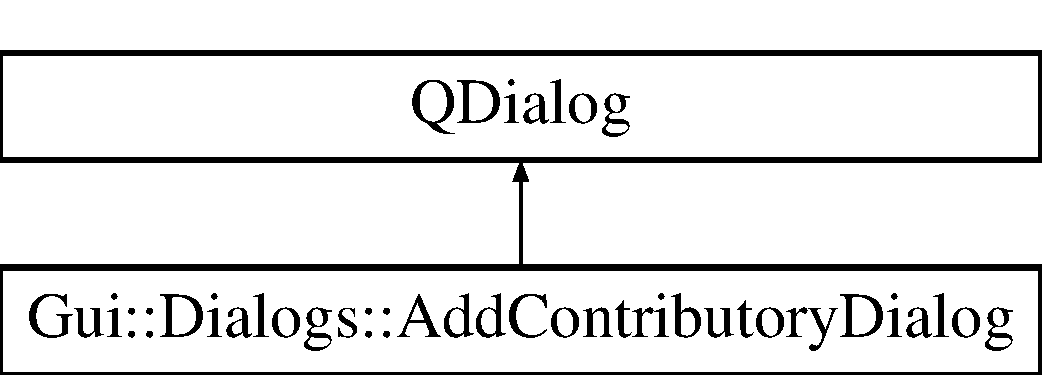
\includegraphics[height=2.000000cm]{d5/de2/classGui_1_1Dialogs_1_1AddContributoryDialog}
\end{center}
\end{figure}
\subsection*{Public Member Functions}
\begin{DoxyCompactItemize}
\item 
\hyperlink{classGui_1_1Dialogs_1_1AddContributoryDialog_a40687642b2f2b15a61298ab18256867a}{Add\-Contributory\-Dialog} (Q\-Widget $\ast$parent=0)
\begin{DoxyCompactList}\small\item\em \hyperlink{classGui_1_1Dialogs_1_1AddContributoryDialog_a40687642b2f2b15a61298ab18256867a}{Add\-Contributory\-Dialog\-::\-Add\-Contributory\-Dialog} Construct a new windows Add\-Contributory. \end{DoxyCompactList}\end{DoxyCompactItemize}


\subsection{Detailed Description}
The \hyperlink{classGui_1_1Dialogs_1_1AddContributoryDialog}{Add\-Contributory\-Dialog} class Windows to add a new Contributory. 

\begin{DoxyAuthor}{Author}
Florent Berbie 
\end{DoxyAuthor}
\begin{DoxySeeAlso}{See Also}
Contributory 
\end{DoxySeeAlso}


\subsection{Constructor \& Destructor Documentation}
\hypertarget{classGui_1_1Dialogs_1_1AddContributoryDialog_a40687642b2f2b15a61298ab18256867a}{\index{Gui\-::\-Dialogs\-::\-Add\-Contributory\-Dialog@{Gui\-::\-Dialogs\-::\-Add\-Contributory\-Dialog}!Add\-Contributory\-Dialog@{Add\-Contributory\-Dialog}}
\index{Add\-Contributory\-Dialog@{Add\-Contributory\-Dialog}!Gui::Dialogs::AddContributoryDialog@{Gui\-::\-Dialogs\-::\-Add\-Contributory\-Dialog}}
\subsubsection[{Add\-Contributory\-Dialog}]{\setlength{\rightskip}{0pt plus 5cm}Gui\-::\-Dialogs\-::\-Add\-Contributory\-Dialog\-::\-Add\-Contributory\-Dialog (
\begin{DoxyParamCaption}
\item[{Q\-Widget $\ast$}]{parent = {\ttfamily 0}}
\end{DoxyParamCaption}
)\hspace{0.3cm}{\ttfamily [explicit]}}}\label{classGui_1_1Dialogs_1_1AddContributoryDialog_a40687642b2f2b15a61298ab18256867a}


\hyperlink{classGui_1_1Dialogs_1_1AddContributoryDialog_a40687642b2f2b15a61298ab18256867a}{Add\-Contributory\-Dialog\-::\-Add\-Contributory\-Dialog} Construct a new windows Add\-Contributory. 


\begin{DoxyParams}{Parameters}
{\em parent} & Q\-Widget \\
\hline
\end{DoxyParams}


The documentation for this class was generated from the following files\-:\begin{DoxyCompactItemize}
\item 
/home/florent/\-Documents/\-Projet\-\_\-\-S8/\-Fact\-Dev/src/gui/dialogs/addcontributorydialog.\-h\item 
/home/florent/\-Documents/\-Projet\-\_\-\-S8/\-Fact\-Dev/src/gui/dialogs/addcontributorydialog.\-cpp\end{DoxyCompactItemize}

\hypertarget{classGui_1_1Dialogs_1_1AddProjectDialog}{\section{Gui\-:\-:Dialogs\-:\-:Add\-Project\-Dialog Class Reference}
\label{classGui_1_1Dialogs_1_1AddProjectDialog}\index{Gui\-::\-Dialogs\-::\-Add\-Project\-Dialog@{Gui\-::\-Dialogs\-::\-Add\-Project\-Dialog}}
}


The \hyperlink{classGui_1_1Dialogs_1_1AddProjectDialog}{Add\-Project\-Dialog} class Windows to add a new Project.  




{\ttfamily \#include $<$addprojectdialog.\-h$>$}

Inheritance diagram for Gui\-:\-:Dialogs\-:\-:Add\-Project\-Dialog\-:\begin{figure}[H]
\begin{center}
\leavevmode
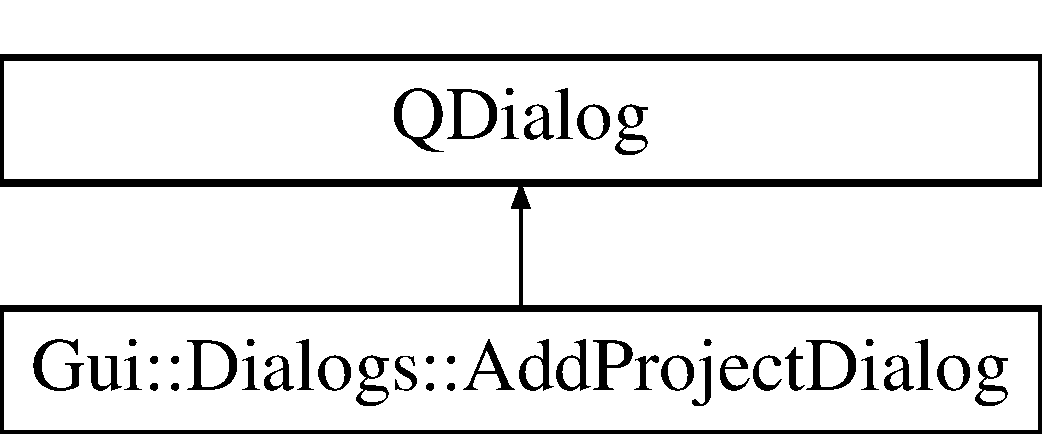
\includegraphics[height=2.000000cm]{de/d36/classGui_1_1Dialogs_1_1AddProjectDialog}
\end{center}
\end{figure}
\subsection*{Public Slots}
\begin{DoxyCompactItemize}
\item 
\hypertarget{classGui_1_1Dialogs_1_1AddProjectDialog_ab30cf2a880e1746cf629a69fb7d9e7f9}{void \hyperlink{classGui_1_1Dialogs_1_1AddProjectDialog_ab30cf2a880e1746cf629a69fb7d9e7f9}{check\-Fields} ()}\label{classGui_1_1Dialogs_1_1AddProjectDialog_ab30cf2a880e1746cf629a69fb7d9e7f9}

\begin{DoxyCompactList}\small\item\em \hyperlink{classGui_1_1Dialogs_1_1AddProjectDialog_ab30cf2a880e1746cf629a69fb7d9e7f9}{Add\-Project\-Dialog\-::check\-Fields} Check if fields are valid. \end{DoxyCompactList}\end{DoxyCompactItemize}
\subsection*{Public Member Functions}
\begin{DoxyCompactItemize}
\item 
\hyperlink{classGui_1_1Dialogs_1_1AddProjectDialog_a1fa86f5366f321233655aaf6923ec892}{Add\-Project\-Dialog} (int id=0, Q\-Widget $\ast$parent=0)
\begin{DoxyCompactList}\small\item\em \hyperlink{classGui_1_1Dialogs_1_1AddProjectDialog_a1fa86f5366f321233655aaf6923ec892}{Add\-Project\-Dialog\-::\-Add\-Project\-Dialog} Construct a windows \hyperlink{classGui_1_1Dialogs_1_1AddProjectDialog}{Add\-Project\-Dialog}. \end{DoxyCompactList}\item 
\hyperlink{classGui_1_1Dialogs_1_1AddProjectDialog_a7433c07961921a18abb56a6aeb741b1f}{Add\-Project\-Dialog} (int no\-Row\-Customer, int id\-Project=0, Q\-Widget $\ast$parent=0)
\begin{DoxyCompactList}\small\item\em Add\-Project\-Dialog\-Add\-Project\-Dialog Construct a windows according an {\itshape id\-Customer} and, optionnaly, an {\itshape id\-Project} \end{DoxyCompactList}\item 
\hypertarget{classGui_1_1Dialogs_1_1AddProjectDialog_abe345ededea4911846a44b984cc04f18}{void \hyperlink{classGui_1_1Dialogs_1_1AddProjectDialog_abe345ededea4911846a44b984cc04f18}{accept} ()}\label{classGui_1_1Dialogs_1_1AddProjectDialog_abe345ededea4911846a44b984cc04f18}

\begin{DoxyCompactList}\small\item\em \hyperlink{classGui_1_1Dialogs_1_1AddProjectDialog_abe345ededea4911846a44b984cc04f18}{Add\-Project\-Dialog\-::accept} Valid data inputed by user and add these data in Database. \end{DoxyCompactList}\item 
\hypertarget{classGui_1_1Dialogs_1_1AddProjectDialog_a767dcea1ae96d2efc3085f8ade4406ce}{void \hyperlink{classGui_1_1Dialogs_1_1AddProjectDialog_a767dcea1ae96d2efc3085f8ade4406ce}{reject} ()}\label{classGui_1_1Dialogs_1_1AddProjectDialog_a767dcea1ae96d2efc3085f8ade4406ce}

\begin{DoxyCompactList}\small\item\em \hyperlink{classGui_1_1Dialogs_1_1AddProjectDialog_a767dcea1ae96d2efc3085f8ade4406ce}{Add\-Project\-Dialog\-::reject} Cancel the operation and close the windows. \end{DoxyCompactList}\item 
\hypertarget{classGui_1_1Dialogs_1_1AddProjectDialog_af31b6ed23acdd5fb8b71caaeddce34f4}{void \hyperlink{classGui_1_1Dialogs_1_1AddProjectDialog_af31b6ed23acdd5fb8b71caaeddce34f4}{fill\-Fields} ()}\label{classGui_1_1Dialogs_1_1AddProjectDialog_af31b6ed23acdd5fb8b71caaeddce34f4}

\begin{DoxyCompactList}\small\item\em \hyperlink{classGui_1_1Dialogs_1_1AddProjectDialog_af31b6ed23acdd5fb8b71caaeddce34f4}{Add\-Project\-Dialog\-::fill\-Fields} Fill the differents fields of the current windows according the Project data existing As a project requires to be linked to a Customer, the Customer selection part may be disable. \end{DoxyCompactList}\end{DoxyCompactItemize}


\subsection{Detailed Description}
The \hyperlink{classGui_1_1Dialogs_1_1AddProjectDialog}{Add\-Project\-Dialog} class Windows to add a new Project. 

\begin{DoxyAuthor}{Author}
Florent Berbie 
\end{DoxyAuthor}
\begin{DoxySeeAlso}{See Also}
Project 
\end{DoxySeeAlso}


\subsection{Constructor \& Destructor Documentation}
\hypertarget{classGui_1_1Dialogs_1_1AddProjectDialog_a1fa86f5366f321233655aaf6923ec892}{\index{Gui\-::\-Dialogs\-::\-Add\-Project\-Dialog@{Gui\-::\-Dialogs\-::\-Add\-Project\-Dialog}!Add\-Project\-Dialog@{Add\-Project\-Dialog}}
\index{Add\-Project\-Dialog@{Add\-Project\-Dialog}!Gui::Dialogs::AddProjectDialog@{Gui\-::\-Dialogs\-::\-Add\-Project\-Dialog}}
\subsubsection[{Add\-Project\-Dialog}]{\setlength{\rightskip}{0pt plus 5cm}Gui\-::\-Dialogs\-::\-Add\-Project\-Dialog\-::\-Add\-Project\-Dialog (
\begin{DoxyParamCaption}
\item[{int}]{id = {\ttfamily 0}, }
\item[{Q\-Widget $\ast$}]{parent = {\ttfamily 0}}
\end{DoxyParamCaption}
)\hspace{0.3cm}{\ttfamily [explicit]}}}\label{classGui_1_1Dialogs_1_1AddProjectDialog_a1fa86f5366f321233655aaf6923ec892}


\hyperlink{classGui_1_1Dialogs_1_1AddProjectDialog_a1fa86f5366f321233655aaf6923ec892}{Add\-Project\-Dialog\-::\-Add\-Project\-Dialog} Construct a windows \hyperlink{classGui_1_1Dialogs_1_1AddProjectDialog}{Add\-Project\-Dialog}. 


\begin{DoxyParams}{Parameters}
{\em id} & Project identity \\
\hline
{\em parent} & Q\-Widget of the current windows \\
\hline
\end{DoxyParams}
\hypertarget{classGui_1_1Dialogs_1_1AddProjectDialog_a7433c07961921a18abb56a6aeb741b1f}{\index{Gui\-::\-Dialogs\-::\-Add\-Project\-Dialog@{Gui\-::\-Dialogs\-::\-Add\-Project\-Dialog}!Add\-Project\-Dialog@{Add\-Project\-Dialog}}
\index{Add\-Project\-Dialog@{Add\-Project\-Dialog}!Gui::Dialogs::AddProjectDialog@{Gui\-::\-Dialogs\-::\-Add\-Project\-Dialog}}
\subsubsection[{Add\-Project\-Dialog}]{\setlength{\rightskip}{0pt plus 5cm}Gui\-::\-Dialogs\-::\-Add\-Project\-Dialog\-::\-Add\-Project\-Dialog (
\begin{DoxyParamCaption}
\item[{int}]{no\-Row\-Customer, }
\item[{int}]{id\-Project = {\ttfamily 0}, }
\item[{Q\-Widget $\ast$}]{parent = {\ttfamily 0}}
\end{DoxyParamCaption}
)\hspace{0.3cm}{\ttfamily [explicit]}}}\label{classGui_1_1Dialogs_1_1AddProjectDialog_a7433c07961921a18abb56a6aeb741b1f}


Add\-Project\-Dialog\-Add\-Project\-Dialog Construct a windows according an {\itshape id\-Customer} and, optionnaly, an {\itshape id\-Project} 


\begin{DoxyParams}{Parameters}
{\em no\-Row\-Customer} & Row number of the Customer \\
\hline
{\em id\-Project} & Project identify \\
\hline
{\em parent} & Q\-Widget of the current windows \\
\hline
\end{DoxyParams}


The documentation for this class was generated from the following files\-:\begin{DoxyCompactItemize}
\item 
/home/florent/\-Documents/\-Projet\-\_\-\-S8/\-Fact\-Dev/src/gui/dialogs/addprojectdialog.\-h\item 
/home/florent/\-Documents/\-Projet\-\_\-\-S8/\-Fact\-Dev/src/gui/dialogs/addprojectdialog.\-cpp\end{DoxyCompactItemize}

\hypertarget{classGui_1_1Dialogs_1_1AddQuoteDialog}{\section{Gui\-:\-:Dialogs\-:\-:Add\-Quote\-Dialog Class Reference}
\label{classGui_1_1Dialogs_1_1AddQuoteDialog}\index{Gui\-::\-Dialogs\-::\-Add\-Quote\-Dialog@{Gui\-::\-Dialogs\-::\-Add\-Quote\-Dialog}}
}


The \hyperlink{classGui_1_1Dialogs_1_1AddQuoteDialog}{Add\-Quote\-Dialog} class Window to add or modify a Quote.  




{\ttfamily \#include $<$addquotedialog.\-h$>$}

Inheritance diagram for Gui\-:\-:Dialogs\-:\-:Add\-Quote\-Dialog\-:\begin{figure}[H]
\begin{center}
\leavevmode
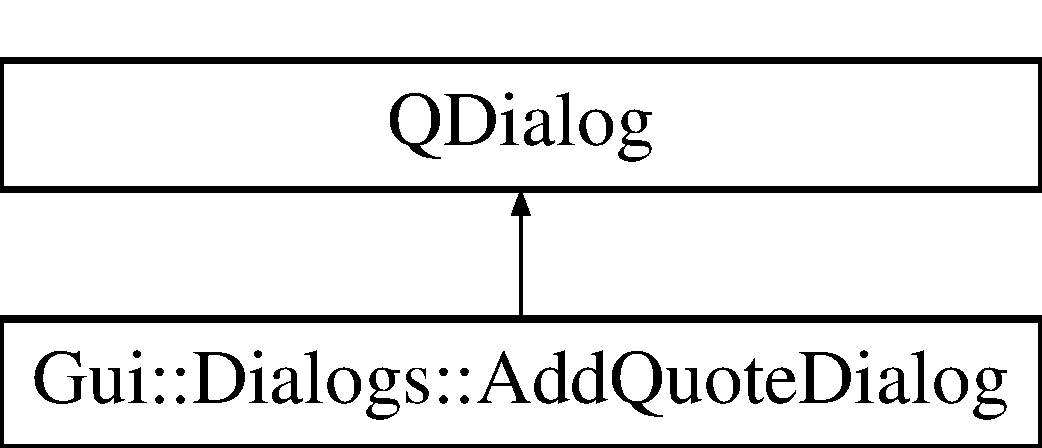
\includegraphics[height=2.000000cm]{d6/d43/classGui_1_1Dialogs_1_1AddQuoteDialog}
\end{center}
\end{figure}
\subsection*{Public Slots}
\begin{DoxyCompactItemize}
\item 
\hypertarget{classGui_1_1Dialogs_1_1AddQuoteDialog_a5fa7b833c2a4271cc637e7dd9ec72fff}{void {\bfseries update\-Btn} (void)}\label{classGui_1_1Dialogs_1_1AddQuoteDialog_a5fa7b833c2a4271cc637e7dd9ec72fff}

\end{DoxyCompactItemize}
\subsection*{Public Member Functions}
\begin{DoxyCompactItemize}
\item 
\hyperlink{classGui_1_1Dialogs_1_1AddQuoteDialog_ae6a6d0730d6ec3804ab802821e89ebd5}{Add\-Quote\-Dialog} (bool is\-Billing, int id\-Customer=0, int id=0, Q\-Widget $\ast$parent=0)
\begin{DoxyCompactList}\small\item\em \hyperlink{classGui_1_1Dialogs_1_1AddQuoteDialog_ae6a6d0730d6ec3804ab802821e89ebd5}{Add\-Quote\-Dialog\-::\-Add\-Quote\-Dialog} Construct a windows \hyperlink{classGui_1_1Dialogs_1_1AddQuoteDialog}{Add\-Quote\-Dialog}. \end{DoxyCompactList}\item 
\hypertarget{classGui_1_1Dialogs_1_1AddQuoteDialog_a5dd0cca14b1172a7e1dd9019d8fa8ff3}{void \hyperlink{classGui_1_1Dialogs_1_1AddQuoteDialog_a5dd0cca14b1172a7e1dd9019d8fa8ff3}{fill\-Fields} ()}\label{classGui_1_1Dialogs_1_1AddQuoteDialog_a5dd0cca14b1172a7e1dd9019d8fa8ff3}

\begin{DoxyCompactList}\small\item\em Add\-Quote\-Dialog\-::\-Fill line edits with the data of the quote. \end{DoxyCompactList}\item 
int \hyperlink{classGui_1_1Dialogs_1_1AddQuoteDialog_a68b6b01e0818cb6615b2335d486aac09}{get\-Number} ()
\begin{DoxyCompactList}\small\item\em \hyperlink{classGui_1_1Dialogs_1_1AddQuoteDialog_a68b6b01e0818cb6615b2335d486aac09}{Add\-Quote\-Dialog\-::get\-Number} return the number of bill or quote. \end{DoxyCompactList}\item 
\hypertarget{classGui_1_1Dialogs_1_1AddQuoteDialog_abcc6fc79a513dd1765a4494d9499586b}{void \hyperlink{classGui_1_1Dialogs_1_1AddQuoteDialog_abcc6fc79a513dd1765a4494d9499586b}{accept} ()}\label{classGui_1_1Dialogs_1_1AddQuoteDialog_abcc6fc79a513dd1765a4494d9499586b}

\begin{DoxyCompactList}\small\item\em \hyperlink{classGui_1_1Dialogs_1_1AddQuoteDialog_abcc6fc79a513dd1765a4494d9499586b}{Add\-Quote\-Dialog\-::accept} Valid data inputed by user and add these data in Database. \end{DoxyCompactList}\item 
\hypertarget{classGui_1_1Dialogs_1_1AddQuoteDialog_a1ae935c40fb54142aad3a610a137bd36}{void \hyperlink{classGui_1_1Dialogs_1_1AddQuoteDialog_a1ae935c40fb54142aad3a610a137bd36}{reject} ()}\label{classGui_1_1Dialogs_1_1AddQuoteDialog_a1ae935c40fb54142aad3a610a137bd36}

\begin{DoxyCompactList}\small\item\em \hyperlink{classGui_1_1Dialogs_1_1AddQuoteDialog_a1ae935c40fb54142aad3a610a137bd36}{Add\-Quote\-Dialog\-::reject} Cancel the operation and close the windows. \end{DoxyCompactList}\end{DoxyCompactItemize}


\subsection{Detailed Description}
The \hyperlink{classGui_1_1Dialogs_1_1AddQuoteDialog}{Add\-Quote\-Dialog} class Window to add or modify a Quote. 

\begin{DoxyAuthor}{Author}

\end{DoxyAuthor}


\subsection{Constructor \& Destructor Documentation}
\hypertarget{classGui_1_1Dialogs_1_1AddQuoteDialog_ae6a6d0730d6ec3804ab802821e89ebd5}{\index{Gui\-::\-Dialogs\-::\-Add\-Quote\-Dialog@{Gui\-::\-Dialogs\-::\-Add\-Quote\-Dialog}!Add\-Quote\-Dialog@{Add\-Quote\-Dialog}}
\index{Add\-Quote\-Dialog@{Add\-Quote\-Dialog}!Gui::Dialogs::AddQuoteDialog@{Gui\-::\-Dialogs\-::\-Add\-Quote\-Dialog}}
\subsubsection[{Add\-Quote\-Dialog}]{\setlength{\rightskip}{0pt plus 5cm}Gui\-::\-Dialogs\-::\-Add\-Quote\-Dialog\-::\-Add\-Quote\-Dialog (
\begin{DoxyParamCaption}
\item[{bool}]{is\-Billing, }
\item[{int}]{id\-Customer = {\ttfamily 0}, }
\item[{int}]{id = {\ttfamily 0}, }
\item[{Q\-Widget $\ast$}]{parent = {\ttfamily 0}}
\end{DoxyParamCaption}
)\hspace{0.3cm}{\ttfamily [explicit]}}}\label{classGui_1_1Dialogs_1_1AddQuoteDialog_ae6a6d0730d6ec3804ab802821e89ebd5}


\hyperlink{classGui_1_1Dialogs_1_1AddQuoteDialog_ae6a6d0730d6ec3804ab802821e89ebd5}{Add\-Quote\-Dialog\-::\-Add\-Quote\-Dialog} Construct a windows \hyperlink{classGui_1_1Dialogs_1_1AddQuoteDialog}{Add\-Quote\-Dialog}. 


\begin{DoxyParams}{Parameters}
{\em parent} & Q\-Widget of the current windows \\
\hline
\end{DoxyParams}


\subsection{Member Function Documentation}
\hypertarget{classGui_1_1Dialogs_1_1AddQuoteDialog_a68b6b01e0818cb6615b2335d486aac09}{\index{Gui\-::\-Dialogs\-::\-Add\-Quote\-Dialog@{Gui\-::\-Dialogs\-::\-Add\-Quote\-Dialog}!get\-Number@{get\-Number}}
\index{get\-Number@{get\-Number}!Gui::Dialogs::AddQuoteDialog@{Gui\-::\-Dialogs\-::\-Add\-Quote\-Dialog}}
\subsubsection[{get\-Number}]{\setlength{\rightskip}{0pt plus 5cm}int Gui\-::\-Dialogs\-::\-Add\-Quote\-Dialog\-::get\-Number (
\begin{DoxyParamCaption}
{}
\end{DoxyParamCaption}
)}}\label{classGui_1_1Dialogs_1_1AddQuoteDialog_a68b6b01e0818cb6615b2335d486aac09}


\hyperlink{classGui_1_1Dialogs_1_1AddQuoteDialog_a68b6b01e0818cb6615b2335d486aac09}{Add\-Quote\-Dialog\-::get\-Number} return the number of bill or quote. 

\begin{DoxyReturn}{Returns}
int 
\end{DoxyReturn}


The documentation for this class was generated from the following files\-:\begin{DoxyCompactItemize}
\item 
/home/travis/build/\-F\-A\-C\-T-\/\-Team/\-Fact\-Dev/src/gui/dialogs/addquotedialog.\-h\item 
/home/travis/build/\-F\-A\-C\-T-\/\-Team/\-Fact\-Dev/src/gui/dialogs/addquotedialog.\-cpp\end{DoxyCompactItemize}

\hypertarget{classModels_1_1Billing}{\section{Models\-:\-:Billing Class Reference}
\label{classModels_1_1Billing}\index{Models\-::\-Billing@{Models\-::\-Billing}}
}


The \hyperlink{classModels_1_1Billing}{Billing} class \-: \hyperlink{classModels_1_1Billing}{Billing} or Quote of a \hyperlink{classModels_1_1Customer}{Customer}.  




{\ttfamily \#include $<$billing.\-h$>$}

Inheritance diagram for Models\-:\-:Billing\-:\begin{figure}[H]
\begin{center}
\leavevmode
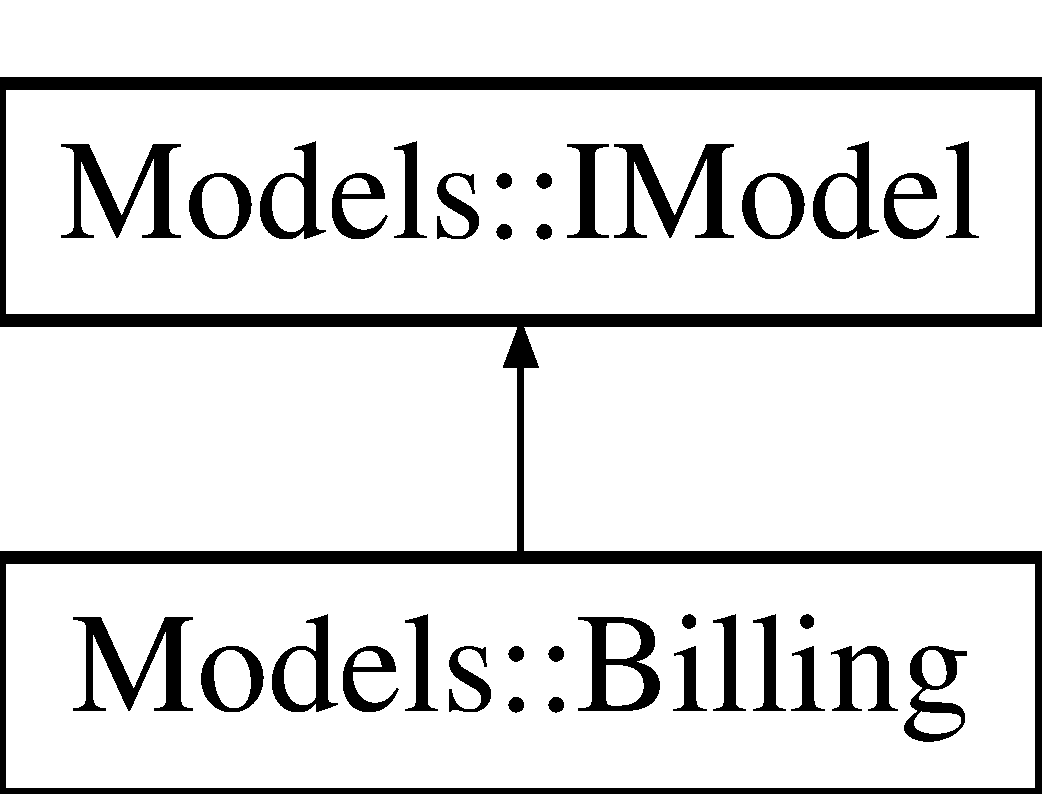
\includegraphics[height=2.000000cm]{d4/d5c/classModels_1_1Billing}
\end{center}
\end{figure}
\subsection*{Public Member Functions}
\begin{DoxyCompactItemize}
\item 
\hypertarget{classModels_1_1Billing_ab6b6e4b21617bacb1e8124b5e1218723}{\hyperlink{classModels_1_1Billing_ab6b6e4b21617bacb1e8124b5e1218723}{Billing} ()}\label{classModels_1_1Billing_ab6b6e4b21617bacb1e8124b5e1218723}

\begin{DoxyCompactList}\small\item\em \hyperlink{classModels_1_1Billing_ab6b6e4b21617bacb1e8124b5e1218723}{Billing\-::\-Billing}. Construct a \hyperlink{classModels_1_1Billing}{Billing}. \end{DoxyCompactList}\item 
\hyperlink{classModels_1_1Billing_a2fba091975b0c62f7e65771e335e038b}{Billing} (int id)
\begin{DoxyCompactList}\small\item\em \hyperlink{classModels_1_1Billing_ab6b6e4b21617bacb1e8124b5e1218723}{Billing\-::\-Billing}. Construct a \hyperlink{classModels_1_1Billing}{Billing} or quote. \end{DoxyCompactList}\item 
\hypertarget{classModels_1_1Billing_a36da0cd70a8f9db9be57bf32f7610e59}{\hyperlink{classModels_1_1Billing_a36da0cd70a8f9db9be57bf32f7610e59}{$\sim$\-Billing} ()}\label{classModels_1_1Billing_a36da0cd70a8f9db9be57bf32f7610e59}

\begin{DoxyCompactList}\small\item\em destruct a billing object \end{DoxyCompactList}\item 
\hypertarget{classModels_1_1Billing_ad2280a0d8dde4c36e88c344b01044caf}{void \hyperlink{classModels_1_1Billing_ad2280a0d8dde4c36e88c344b01044caf}{commit} ()}\label{classModels_1_1Billing_ad2280a0d8dde4c36e88c344b01044caf}

\begin{DoxyCompactList}\small\item\em \hyperlink{classModels_1_1Billing_ad2280a0d8dde4c36e88c344b01044caf}{Billing\-::commit}. Insert a modification in \hyperlink{classModels_1_1Billing}{Billing} table on the database. \end{DoxyCompactList}\item 
void \hyperlink{classModels_1_1Billing_a689643008955fdcd5833631a6202c0dc}{hydrat} (int \hyperlink{classModels_1_1IModel_a63087bb34da8c38a11109cd775122d31}{get\-Id})
\begin{DoxyCompactList}\small\item\em \hyperlink{classModels_1_1Billing_a689643008955fdcd5833631a6202c0dc}{Billing\-::hydrat}. Update of the \hyperlink{classModels_1_1Billing}{Billing} which is specified by {\itshape get\-Id} \end{DoxyCompactList}\item 
\hypertarget{classModels_1_1Billing_ada8a7c127a80fa7349fbd6a7d30ca4a3}{void \hyperlink{classModels_1_1Billing_ada8a7c127a80fa7349fbd6a7d30ca4a3}{remove} ()}\label{classModels_1_1Billing_ada8a7c127a80fa7349fbd6a7d30ca4a3}

\begin{DoxyCompactList}\small\item\em \hyperlink{classModels_1_1Billing_ada8a7c127a80fa7349fbd6a7d30ca4a3}{Billing\-::remove}. Remove a \hyperlink{classModels_1_1Billing}{Billing}. \end{DoxyCompactList}\item 
Q\-Variant\-Hash \hyperlink{classModels_1_1Billing_a2363c0b978434c0a835f894a67eb81e1}{get\-Data\-Map} ()
\begin{DoxyCompactList}\small\item\em \hyperlink{classModels_1_1Billing_a2363c0b978434c0a835f894a67eb81e1}{Billing\-::get\-Data\-Map} Get all data of model with a Hash\-Map key/value. \end{DoxyCompactList}\item 
double \hyperlink{classModels_1_1Billing_a866e81394fa11dce7dc4ab7bfc53ed79}{get\-Price} (bool paied=false)
\begin{DoxyCompactList}\small\item\em get\-Price Return the price of a calculable object \end{DoxyCompactList}\item 
double \hyperlink{classModels_1_1Billing_a360006189d4867e3281009b0c465bc53}{get\-Sum\-Quantity} ()
\begin{DoxyCompactList}\small\item\em \hyperlink{classModels_1_1ContributoriesList_af9b3b1b703cebeef552d058999ffcc4c}{Contributories\-List\-::get\-Sum\-Quantity} Return the sum of quantity (number of days) of the Contributories. \end{DoxyCompactList}\item 
\hypertarget{classModels_1_1Billing_a3f835c6f4ea0b66c43bb7fec40c6e075}{void \hyperlink{classModels_1_1Billing_a3f835c6f4ea0b66c43bb7fec40c6e075}{generate\-Tex} ()}\label{classModels_1_1Billing_a3f835c6f4ea0b66c43bb7fec40c6e075}

\begin{DoxyCompactList}\small\item\em \hyperlink{classModels_1_1Billing_a3f835c6f4ea0b66c43bb7fec40c6e075}{Billing\-::generate\-Tex} Generate a .tex file for the billing. \end{DoxyCompactList}\item 
\hypertarget{classModels_1_1Billing_a27e273242564cdb68c14810a4580f8e5}{void \hyperlink{classModels_1_1Billing_a27e273242564cdb68c14810a4580f8e5}{generate\-Pdf} ()}\label{classModels_1_1Billing_a27e273242564cdb68c14810a4580f8e5}

\begin{DoxyCompactList}\small\item\em \hyperlink{classModels_1_1Billing_a27e273242564cdb68c14810a4580f8e5}{Billing\-::generate\-Pdf} Generate a .pdf file for the billing. \end{DoxyCompactList}\item 
Q\-String \hyperlink{classModels_1_1Billing_a4110ac32d8d96b9fbd1b0037df39723b}{get\-Path} ()
\begin{DoxyCompactList}\small\item\em \hyperlink{classModels_1_1Billing_a4110ac32d8d96b9fbd1b0037df39723b}{Billing\-::get\-Path} Return the path of billing filename (without extension) \end{DoxyCompactList}\item 
Q\-String \hyperlink{classModels_1_1Billing_a2359afe641ba85a37729fb0d951bff7d}{get\-Folder} ()
\begin{DoxyCompactList}\small\item\em \hyperlink{classModels_1_1Billing_a2359afe641ba85a37729fb0d951bff7d}{Billing\-::get\-Folder} Return the directory of billing. \end{DoxyCompactList}\item 
Q\-String \hyperlink{classModels_1_1Billing_ae8700d38ecd8e4975f1ee013144ed455}{get\-Filename} ()
\begin{DoxyCompactList}\small\item\em \hyperlink{classModels_1_1Billing_ae8700d38ecd8e4975f1ee013144ed455}{Billing\-::get\-Filename} Return the filename of billing (without extension) \end{DoxyCompactList}\item 
\hyperlink{classModels_1_1ContributoriesList}{Contributories\-List} \& \hyperlink{classModels_1_1Billing_af3d66c06d8c4d855b0efa5ff599a3ceb}{get\-Contributories} ()
\begin{DoxyCompactList}\small\item\em \hyperlink{classModels_1_1Billing_af3d66c06d8c4d855b0efa5ff599a3ceb}{Billing\-::get\-Contributories}. Return a map of {\bfseries \hyperlink{classModels_1_1Contributory}{Contributory}} for each {\bfseries \hyperlink{classModels_1_1Project}{Project}} of the {\bfseries \hyperlink{classModels_1_1Billing}{Billing}} \end{DoxyCompactList}\item 
void \hyperlink{classModels_1_1Billing_a3636d785d2cb77d83d21a795e1f91a60}{add\-Contributory} (\hyperlink{classModels_1_1Contributory}{Contributory} \&c)
\begin{DoxyCompactList}\small\item\em Billing\-::add\-Contributories Add a new contributory for project p. \end{DoxyCompactList}\item 
Q\-String \hyperlink{classModels_1_1Billing_a15cd358ce3cab05668c62c0771afdb85}{get\-Title} () const 
\begin{DoxyCompactList}\small\item\em \hyperlink{classModels_1_1Billing_a15cd358ce3cab05668c62c0771afdb85}{Billing\-::get\-Title}. return title of {\bfseries \hyperlink{classModels_1_1Billing}{Billing}} \end{DoxyCompactList}\item 
void \hyperlink{classModels_1_1Billing_ae20cea169abdffa5daaa368547425928}{set\-Title} (const Q\-String \&\hyperlink{classModels_1_1Billing_a15cd358ce3cab05668c62c0771afdb85}{get\-Title})
\begin{DoxyCompactList}\small\item\em \hyperlink{classModels_1_1Billing_ae20cea169abdffa5daaa368547425928}{Billing\-::set\-Title}. Modify the title of {\bfseries \hyperlink{classModels_1_1Billing}{Billing}} \end{DoxyCompactList}\item 
Q\-String \hyperlink{classModels_1_1Billing_a5802215da8f4407457b8aeb7be525c65}{get\-Description} () const 
\begin{DoxyCompactList}\small\item\em \hyperlink{classModels_1_1Billing_a5802215da8f4407457b8aeb7be525c65}{Billing\-::get\-Description}. return description of {\bfseries \hyperlink{classModels_1_1Billing}{Billing}} \end{DoxyCompactList}\item 
void \hyperlink{classModels_1_1Billing_adb5cf4382150387f10bb6b774ace6bc8}{set\-Description} (const Q\-String \&\hyperlink{classModels_1_1Billing_a5802215da8f4407457b8aeb7be525c65}{get\-Description})
\begin{DoxyCompactList}\small\item\em \hyperlink{classModels_1_1Billing_adb5cf4382150387f10bb6b774ace6bc8}{Billing\-::set\-Description}. Modify the description of {\bfseries \hyperlink{classModels_1_1Billing}{Billing}} \end{DoxyCompactList}\item 
int \hyperlink{classModels_1_1Billing_a48c6e28a4aec13f8ed6b3ebbab837f0b}{get\-Number} () const 
\begin{DoxyCompactList}\small\item\em \hyperlink{classModels_1_1Billing_a48c6e28a4aec13f8ed6b3ebbab837f0b}{Billing\-::get\-Number}. Return number of the {\bfseries \hyperlink{classModels_1_1Billing}{Billing}}. \end{DoxyCompactList}\item 
void \hyperlink{classModels_1_1Billing_a2b43e0c657a9e717c9d2c091d222369e}{set\-Number} (int \hyperlink{classModels_1_1Billing_a48c6e28a4aec13f8ed6b3ebbab837f0b}{get\-Number})
\begin{DoxyCompactList}\small\item\em \hyperlink{classModels_1_1Billing_a2b43e0c657a9e717c9d2c091d222369e}{Billing\-::set\-Number}. Modify {\itshape \-\_\-number} of \hyperlink{classModels_1_1Billing}{Billing}. \end{DoxyCompactList}\item 
bool \hyperlink{classModels_1_1Billing_ab03dd29a9812a995355a1d93318f348f}{is\-Billing} () const 
\begin{DoxyCompactList}\small\item\em \hyperlink{classModels_1_1Billing_ab03dd29a9812a995355a1d93318f348f}{Billing\-::is\-Billing}. Return if it's a billing or a quote. \end{DoxyCompactList}\item 
void \hyperlink{classModels_1_1Billing_aff8b71426c02bc97f0a724ef762cd42e}{set\-Is\-Billing} (bool \hyperlink{classModels_1_1Billing_ab03dd29a9812a995355a1d93318f348f}{is\-Billing})
\begin{DoxyCompactList}\small\item\em \hyperlink{classModels_1_1Billing_aff8b71426c02bc97f0a724ef762cd42e}{Billing\-::set\-Is\-Billing}. Modify {\itshape is\-Billing} of {\bfseries \hyperlink{classModels_1_1Billing}{Billing}}. \end{DoxyCompactList}\item 
Q\-Date \hyperlink{classModels_1_1Billing_af0d1f0132d0902fb96456d0a9018b701}{get\-Date} () const 
\begin{DoxyCompactList}\small\item\em \hyperlink{classModels_1_1Billing_af0d1f0132d0902fb96456d0a9018b701}{Billing\-::get\-Date}. return date of the {\bfseries \hyperlink{classModels_1_1Billing}{Billing}} \end{DoxyCompactList}\item 
void \hyperlink{classModels_1_1Billing_ae8db0fe5fe273fad31e2f846b5b891cb}{set\-Date} (const Q\-Date \&\hyperlink{classModels_1_1Billing_af0d1f0132d0902fb96456d0a9018b701}{get\-Date})
\begin{DoxyCompactList}\small\item\em \hyperlink{classModels_1_1Billing_ae8db0fe5fe273fad31e2f846b5b891cb}{Billing\-::set\-Date}. Modify {\itshape date} of the {\bfseries \hyperlink{classModels_1_1Billing}{Billing}} \end{DoxyCompactList}\item 
bool \hyperlink{classModels_1_1Billing_ab2f9bd62e920be8c68313e35bbcabd46}{is\-Paid} () const 
\begin{DoxyCompactList}\small\item\em \hyperlink{classModels_1_1Billing_ab2f9bd62e920be8c68313e35bbcabd46}{Billing\-::is\-Paid} Return T\-R\-U\-E if thee current billing is paid else return F\-A\-L\-S\-E. \end{DoxyCompactList}\item 
void \hyperlink{classModels_1_1Billing_a99cf8c1b7435fe268b8fa9257cad6c56}{set\-Is\-Paid} (bool \hyperlink{classModels_1_1Billing_ab2f9bd62e920be8c68313e35bbcabd46}{is\-Paid})
\begin{DoxyCompactList}\small\item\em \hyperlink{classModels_1_1Billing_a99cf8c1b7435fe268b8fa9257cad6c56}{Billing\-::set\-Is\-Paid} Define the current billing according the argument {\itshape is\-Paid} \end{DoxyCompactList}\item 
bool \hyperlink{classModels_1_1Billing_af3d8818a1e00eaa707058567fccf045b}{operator==} (const \hyperlink{classModels_1_1Billing}{Billing} \&b)
\begin{DoxyCompactList}\small\item\em \hyperlink{classModels_1_1Billing_af3d8818a1e00eaa707058567fccf045b}{Billing\-::operator ==} define the operator \char`\"{}==\char`\"{} to compare two billings and to see if they are the same. \end{DoxyCompactList}\item 
bool \hyperlink{classModels_1_1Billing_ae6ff88e05384718d57be1be38f250a52}{operator!=} (const \hyperlink{classModels_1_1Billing}{Billing} \&b)
\begin{DoxyCompactList}\small\item\em \hyperlink{classModels_1_1Billing_ae6ff88e05384718d57be1be38f250a52}{Billing\-::operator !=} defines the operator \char`\"{}!=\char`\"{} to compare two {\bfseries \hyperlink{classModels_1_1Billing}{Billing}} and to see if they are different. \end{DoxyCompactList}\item 
\hypertarget{classModels_1_1Billing_acb836caf7aef8e953c432661cb8aa55f}{void {\bfseries set\-Contributories} (const \hyperlink{classModels_1_1ContributoriesList}{Contributories\-List} \&contributories)}\label{classModels_1_1Billing_acb836caf7aef8e953c432661cb8aa55f}

\item 
bool \hyperlink{classModels_1_1Billing_a6d3f5da2e9a0b7de217dc51220c4c7b7}{operator$<$} (const \hyperlink{classModels_1_1Billing}{Billing} \&b) const 
\begin{DoxyCompactList}\small\item\em \hyperlink{classModels_1_1Billing_a6d3f5da2e9a0b7de217dc51220c4c7b7}{Billing\-::operator $<$} defines the operator "$<$ to compare two {\bfseries \hyperlink{classModels_1_1Billing}{Billing}} and to see if the fisrt is anterior to the second. \end{DoxyCompactList}\item 
Q\-Standard\-Item $\ast$ \hyperlink{classModels_1_1Billing_ad45495eafb4f67434b69af916e343ac6}{get\-Item} ()
\begin{DoxyCompactList}\small\item\em \hyperlink{classModels_1_1Billing_ad45495eafb4f67434b69af916e343ac6}{Billing\-::get\-Item} Return the bill/quote item. \end{DoxyCompactList}\end{DoxyCompactItemize}
\subsection*{Additional Inherited Members}


\subsection{Detailed Description}
The \hyperlink{classModels_1_1Billing}{Billing} class \-: \hyperlink{classModels_1_1Billing}{Billing} or Quote of a \hyperlink{classModels_1_1Customer}{Customer}. 

\begin{DoxyAuthor}{Author}
Antoine de Roquemaurel 

Florent Berbie 
\end{DoxyAuthor}


\subsection{Constructor \& Destructor Documentation}
\hypertarget{classModels_1_1Billing_a2fba091975b0c62f7e65771e335e038b}{\index{Models\-::\-Billing@{Models\-::\-Billing}!Billing@{Billing}}
\index{Billing@{Billing}!Models::Billing@{Models\-::\-Billing}}
\subsubsection[{Billing}]{\setlength{\rightskip}{0pt plus 5cm}Models\-::\-Billing\-::\-Billing (
\begin{DoxyParamCaption}
\item[{int}]{id}
\end{DoxyParamCaption}
)}}\label{classModels_1_1Billing_a2fba091975b0c62f7e65771e335e038b}


\hyperlink{classModels_1_1Billing_ab6b6e4b21617bacb1e8124b5e1218723}{Billing\-::\-Billing}. Construct a \hyperlink{classModels_1_1Billing}{Billing} or quote. 


\begin{DoxyParams}{Parameters}
{\em int} & id \\
\hline
\end{DoxyParams}


\subsection{Member Function Documentation}
\hypertarget{classModels_1_1Billing_a3636d785d2cb77d83d21a795e1f91a60}{\index{Models\-::\-Billing@{Models\-::\-Billing}!add\-Contributory@{add\-Contributory}}
\index{add\-Contributory@{add\-Contributory}!Models::Billing@{Models\-::\-Billing}}
\subsubsection[{add\-Contributory}]{\setlength{\rightskip}{0pt plus 5cm}void Models\-::\-Billing\-::add\-Contributory (
\begin{DoxyParamCaption}
\item[{{\bf Contributory} \&}]{c}
\end{DoxyParamCaption}
)}}\label{classModels_1_1Billing_a3636d785d2cb77d83d21a795e1f91a60}


Billing\-::add\-Contributories Add a new contributory for project p. 


\begin{DoxyParams}{Parameters}
{\em p} & The \hyperlink{classModels_1_1Project}{Project} who contain \hyperlink{classModels_1_1Contributory}{Contributory} \\
\hline
{\em c} & The new \hyperlink{classModels_1_1Contributory}{Contributory} \\
\hline
\end{DoxyParams}
\hypertarget{classModels_1_1Billing_af3d66c06d8c4d855b0efa5ff599a3ceb}{\index{Models\-::\-Billing@{Models\-::\-Billing}!get\-Contributories@{get\-Contributories}}
\index{get\-Contributories@{get\-Contributories}!Models::Billing@{Models\-::\-Billing}}
\subsubsection[{get\-Contributories}]{\setlength{\rightskip}{0pt plus 5cm}{\bf Contributories\-List} \& Models\-::\-Billing\-::get\-Contributories (
\begin{DoxyParamCaption}
{}
\end{DoxyParamCaption}
)}}\label{classModels_1_1Billing_af3d66c06d8c4d855b0efa5ff599a3ceb}


\hyperlink{classModels_1_1Billing_af3d66c06d8c4d855b0efa5ff599a3ceb}{Billing\-::get\-Contributories}. Return a map of {\bfseries \hyperlink{classModels_1_1Contributory}{Contributory}} for each {\bfseries \hyperlink{classModels_1_1Project}{Project}} of the {\bfseries \hyperlink{classModels_1_1Billing}{Billing}} 

\begin{DoxyReturn}{Returns}
Q\-Map$<$\hyperlink{classModels_1_1Project}{Project}, Q\-List$<$\-Contributory$>$$>$ 
\end{DoxyReturn}
\hypertarget{classModels_1_1Billing_a2363c0b978434c0a835f894a67eb81e1}{\index{Models\-::\-Billing@{Models\-::\-Billing}!get\-Data\-Map@{get\-Data\-Map}}
\index{get\-Data\-Map@{get\-Data\-Map}!Models::Billing@{Models\-::\-Billing}}
\subsubsection[{get\-Data\-Map}]{\setlength{\rightskip}{0pt plus 5cm}Q\-Variant\-Hash Models\-::\-Billing\-::get\-Data\-Map (
\begin{DoxyParamCaption}
{}
\end{DoxyParamCaption}
)\hspace{0.3cm}{\ttfamily [virtual]}}}\label{classModels_1_1Billing_a2363c0b978434c0a835f894a67eb81e1}


\hyperlink{classModels_1_1Billing_a2363c0b978434c0a835f894a67eb81e1}{Billing\-::get\-Data\-Map} Get all data of model with a Hash\-Map key/value. 

\begin{DoxyReturn}{Returns}
Model's data 
\end{DoxyReturn}


Implements \hyperlink{classModels_1_1IModel_a9851b0f296aac58353edff22af11cf3c}{Models\-::\-I\-Model}.

\hypertarget{classModels_1_1Billing_af0d1f0132d0902fb96456d0a9018b701}{\index{Models\-::\-Billing@{Models\-::\-Billing}!get\-Date@{get\-Date}}
\index{get\-Date@{get\-Date}!Models::Billing@{Models\-::\-Billing}}
\subsubsection[{get\-Date}]{\setlength{\rightskip}{0pt plus 5cm}Q\-Date Models\-::\-Billing\-::get\-Date (
\begin{DoxyParamCaption}
{}
\end{DoxyParamCaption}
) const}}\label{classModels_1_1Billing_af0d1f0132d0902fb96456d0a9018b701}


\hyperlink{classModels_1_1Billing_af0d1f0132d0902fb96456d0a9018b701}{Billing\-::get\-Date}. return date of the {\bfseries \hyperlink{classModels_1_1Billing}{Billing}} 

\begin{DoxyReturn}{Returns}
date of \hyperlink{classModels_1_1Billing}{Billing} 
\end{DoxyReturn}
\hypertarget{classModels_1_1Billing_a5802215da8f4407457b8aeb7be525c65}{\index{Models\-::\-Billing@{Models\-::\-Billing}!get\-Description@{get\-Description}}
\index{get\-Description@{get\-Description}!Models::Billing@{Models\-::\-Billing}}
\subsubsection[{get\-Description}]{\setlength{\rightskip}{0pt plus 5cm}Q\-String Models\-::\-Billing\-::get\-Description (
\begin{DoxyParamCaption}
{}
\end{DoxyParamCaption}
) const}}\label{classModels_1_1Billing_a5802215da8f4407457b8aeb7be525c65}


\hyperlink{classModels_1_1Billing_a5802215da8f4407457b8aeb7be525c65}{Billing\-::get\-Description}. return description of {\bfseries \hyperlink{classModels_1_1Billing}{Billing}} 

\begin{DoxyReturn}{Returns}
description of \hyperlink{classModels_1_1Billing}{Billing} 
\end{DoxyReturn}
\hypertarget{classModels_1_1Billing_ae8700d38ecd8e4975f1ee013144ed455}{\index{Models\-::\-Billing@{Models\-::\-Billing}!get\-Filename@{get\-Filename}}
\index{get\-Filename@{get\-Filename}!Models::Billing@{Models\-::\-Billing}}
\subsubsection[{get\-Filename}]{\setlength{\rightskip}{0pt plus 5cm}Q\-String Models\-::\-Billing\-::get\-Filename (
\begin{DoxyParamCaption}
{}
\end{DoxyParamCaption}
)}}\label{classModels_1_1Billing_ae8700d38ecd8e4975f1ee013144ed455}


\hyperlink{classModels_1_1Billing_ae8700d38ecd8e4975f1ee013144ed455}{Billing\-::get\-Filename} Return the filename of billing (without extension) 

\begin{DoxyReturn}{Returns}
Filename of Bulling 
\end{DoxyReturn}
\hypertarget{classModels_1_1Billing_a2359afe641ba85a37729fb0d951bff7d}{\index{Models\-::\-Billing@{Models\-::\-Billing}!get\-Folder@{get\-Folder}}
\index{get\-Folder@{get\-Folder}!Models::Billing@{Models\-::\-Billing}}
\subsubsection[{get\-Folder}]{\setlength{\rightskip}{0pt plus 5cm}Q\-String Models\-::\-Billing\-::get\-Folder (
\begin{DoxyParamCaption}
{}
\end{DoxyParamCaption}
)}}\label{classModels_1_1Billing_a2359afe641ba85a37729fb0d951bff7d}


\hyperlink{classModels_1_1Billing_a2359afe641ba85a37729fb0d951bff7d}{Billing\-::get\-Folder} Return the directory of billing. 

\begin{DoxyReturn}{Returns}
\hyperlink{classModels_1_1Billing}{Billing} directory 
\end{DoxyReturn}
\hypertarget{classModels_1_1Billing_ad45495eafb4f67434b69af916e343ac6}{\index{Models\-::\-Billing@{Models\-::\-Billing}!get\-Item@{get\-Item}}
\index{get\-Item@{get\-Item}!Models::Billing@{Models\-::\-Billing}}
\subsubsection[{get\-Item}]{\setlength{\rightskip}{0pt plus 5cm}Q\-Standard\-Item $\ast$ Models\-::\-Billing\-::get\-Item (
\begin{DoxyParamCaption}
{}
\end{DoxyParamCaption}
)}}\label{classModels_1_1Billing_ad45495eafb4f67434b69af916e343ac6}


\hyperlink{classModels_1_1Billing_ad45495eafb4f67434b69af916e343ac6}{Billing\-::get\-Item} Return the bill/quote item. 

\begin{DoxyReturn}{Returns}
Q\-Standard\-Item an item for Q\-Tree (level/depth 3) 
\end{DoxyReturn}
\hypertarget{classModels_1_1Billing_a48c6e28a4aec13f8ed6b3ebbab837f0b}{\index{Models\-::\-Billing@{Models\-::\-Billing}!get\-Number@{get\-Number}}
\index{get\-Number@{get\-Number}!Models::Billing@{Models\-::\-Billing}}
\subsubsection[{get\-Number}]{\setlength{\rightskip}{0pt plus 5cm}int Models\-::\-Billing\-::get\-Number (
\begin{DoxyParamCaption}
{}
\end{DoxyParamCaption}
) const}}\label{classModels_1_1Billing_a48c6e28a4aec13f8ed6b3ebbab837f0b}


\hyperlink{classModels_1_1Billing_a48c6e28a4aec13f8ed6b3ebbab837f0b}{Billing\-::get\-Number}. Return number of the {\bfseries \hyperlink{classModels_1_1Billing}{Billing}}. 

\begin{DoxyReturn}{Returns}
\-\_\-number of \hyperlink{classModels_1_1Billing}{Billing} 
\end{DoxyReturn}
\hypertarget{classModels_1_1Billing_a4110ac32d8d96b9fbd1b0037df39723b}{\index{Models\-::\-Billing@{Models\-::\-Billing}!get\-Path@{get\-Path}}
\index{get\-Path@{get\-Path}!Models::Billing@{Models\-::\-Billing}}
\subsubsection[{get\-Path}]{\setlength{\rightskip}{0pt plus 5cm}Q\-String Models\-::\-Billing\-::get\-Path (
\begin{DoxyParamCaption}
{}
\end{DoxyParamCaption}
)}}\label{classModels_1_1Billing_a4110ac32d8d96b9fbd1b0037df39723b}


\hyperlink{classModels_1_1Billing_a4110ac32d8d96b9fbd1b0037df39723b}{Billing\-::get\-Path} Return the path of billing filename (without extension) 

\begin{DoxyReturn}{Returns}
billing path 
\end{DoxyReturn}
\hypertarget{classModels_1_1Billing_a866e81394fa11dce7dc4ab7bfc53ed79}{\index{Models\-::\-Billing@{Models\-::\-Billing}!get\-Price@{get\-Price}}
\index{get\-Price@{get\-Price}!Models::Billing@{Models\-::\-Billing}}
\subsubsection[{get\-Price}]{\setlength{\rightskip}{0pt plus 5cm}double Models\-::\-Billing\-::get\-Price (
\begin{DoxyParamCaption}
\item[{bool}]{paied = {\ttfamily false}}
\end{DoxyParamCaption}
)\hspace{0.3cm}{\ttfamily [virtual]}}}\label{classModels_1_1Billing_a866e81394fa11dce7dc4ab7bfc53ed79}


get\-Price Return the price of a calculable object 

\begin{DoxyReturn}{Returns}
The price 
\end{DoxyReturn}


Implements \hyperlink{classModels_1_1Calculable_a5267ee09fc9284063a9fc874b4cc68dc}{Models\-::\-Calculable}.

\hypertarget{classModels_1_1Billing_a360006189d4867e3281009b0c465bc53}{\index{Models\-::\-Billing@{Models\-::\-Billing}!get\-Sum\-Quantity@{get\-Sum\-Quantity}}
\index{get\-Sum\-Quantity@{get\-Sum\-Quantity}!Models::Billing@{Models\-::\-Billing}}
\subsubsection[{get\-Sum\-Quantity}]{\setlength{\rightskip}{0pt plus 5cm}double Models\-::\-Billing\-::get\-Sum\-Quantity (
\begin{DoxyParamCaption}
{}
\end{DoxyParamCaption}
)\hspace{0.3cm}{\ttfamily [virtual]}}}\label{classModels_1_1Billing_a360006189d4867e3281009b0c465bc53}


\hyperlink{classModels_1_1ContributoriesList_af9b3b1b703cebeef552d058999ffcc4c}{Contributories\-List\-::get\-Sum\-Quantity} Return the sum of quantity (number of days) of the Contributories. 

\begin{DoxyReturn}{Returns}
sum of quantity in days 
\end{DoxyReturn}


Implements \hyperlink{classModels_1_1Calculable_a4f9d590b39bd1f0d9e026ac86f1fada1}{Models\-::\-Calculable}.

\hypertarget{classModels_1_1Billing_a15cd358ce3cab05668c62c0771afdb85}{\index{Models\-::\-Billing@{Models\-::\-Billing}!get\-Title@{get\-Title}}
\index{get\-Title@{get\-Title}!Models::Billing@{Models\-::\-Billing}}
\subsubsection[{get\-Title}]{\setlength{\rightskip}{0pt plus 5cm}Q\-String Models\-::\-Billing\-::get\-Title (
\begin{DoxyParamCaption}
{}
\end{DoxyParamCaption}
) const}}\label{classModels_1_1Billing_a15cd358ce3cab05668c62c0771afdb85}


\hyperlink{classModels_1_1Billing_a15cd358ce3cab05668c62c0771afdb85}{Billing\-::get\-Title}. return title of {\bfseries \hyperlink{classModels_1_1Billing}{Billing}} 

\begin{DoxyReturn}{Returns}
title of \hyperlink{classModels_1_1Billing}{Billing} 
\end{DoxyReturn}
\hypertarget{classModels_1_1Billing_a689643008955fdcd5833631a6202c0dc}{\index{Models\-::\-Billing@{Models\-::\-Billing}!hydrat@{hydrat}}
\index{hydrat@{hydrat}!Models::Billing@{Models\-::\-Billing}}
\subsubsection[{hydrat}]{\setlength{\rightskip}{0pt plus 5cm}void Models\-::\-Billing\-::hydrat (
\begin{DoxyParamCaption}
\item[{int}]{get\-Id}
\end{DoxyParamCaption}
)\hspace{0.3cm}{\ttfamily [virtual]}}}\label{classModels_1_1Billing_a689643008955fdcd5833631a6202c0dc}


\hyperlink{classModels_1_1Billing_a689643008955fdcd5833631a6202c0dc}{Billing\-::hydrat}. Update of the \hyperlink{classModels_1_1Billing}{Billing} which is specified by {\itshape get\-Id} 


\begin{DoxyParams}{Parameters}
{\em get\-Id} & \\
\hline
\end{DoxyParams}


Implements \hyperlink{classModels_1_1IModel_a7ce6def437f5e1f6a78ee1d67ca028e4}{Models\-::\-I\-Model}.

\hypertarget{classModels_1_1Billing_ab03dd29a9812a995355a1d93318f348f}{\index{Models\-::\-Billing@{Models\-::\-Billing}!is\-Billing@{is\-Billing}}
\index{is\-Billing@{is\-Billing}!Models::Billing@{Models\-::\-Billing}}
\subsubsection[{is\-Billing}]{\setlength{\rightskip}{0pt plus 5cm}bool Models\-::\-Billing\-::is\-Billing (
\begin{DoxyParamCaption}
{}
\end{DoxyParamCaption}
) const}}\label{classModels_1_1Billing_ab03dd29a9812a995355a1d93318f348f}


\hyperlink{classModels_1_1Billing_ab03dd29a9812a995355a1d93318f348f}{Billing\-::is\-Billing}. Return if it's a billing or a quote. 

\begin{DoxyReturn}{Returns}
if it's billing or a quote 
\end{DoxyReturn}
\hypertarget{classModels_1_1Billing_ab2f9bd62e920be8c68313e35bbcabd46}{\index{Models\-::\-Billing@{Models\-::\-Billing}!is\-Paid@{is\-Paid}}
\index{is\-Paid@{is\-Paid}!Models::Billing@{Models\-::\-Billing}}
\subsubsection[{is\-Paid}]{\setlength{\rightskip}{0pt plus 5cm}bool Models\-::\-Billing\-::is\-Paid (
\begin{DoxyParamCaption}
{}
\end{DoxyParamCaption}
) const}}\label{classModels_1_1Billing_ab2f9bd62e920be8c68313e35bbcabd46}


\hyperlink{classModels_1_1Billing_ab2f9bd62e920be8c68313e35bbcabd46}{Billing\-::is\-Paid} Return T\-R\-U\-E if thee current billing is paid else return F\-A\-L\-S\-E. 

\begin{DoxyReturn}{Returns}
Boolean 
\end{DoxyReturn}
\hypertarget{classModels_1_1Billing_ae6ff88e05384718d57be1be38f250a52}{\index{Models\-::\-Billing@{Models\-::\-Billing}!operator!=@{operator!=}}
\index{operator!=@{operator!=}!Models::Billing@{Models\-::\-Billing}}
\subsubsection[{operator!=}]{\setlength{\rightskip}{0pt plus 5cm}bool Models\-::\-Billing\-::operator!= (
\begin{DoxyParamCaption}
\item[{const {\bf Billing} \&}]{b}
\end{DoxyParamCaption}
)}}\label{classModels_1_1Billing_ae6ff88e05384718d57be1be38f250a52}


\hyperlink{classModels_1_1Billing_ae6ff88e05384718d57be1be38f250a52}{Billing\-::operator !=} defines the operator \char`\"{}!=\char`\"{} to compare two {\bfseries \hyperlink{classModels_1_1Billing}{Billing}} and to see if they are different. 


\begin{DoxyParams}{Parameters}
{\em b} & the {\bfseries \hyperlink{classModels_1_1Billing}{Billing}} to compare with the current {\bfseries \hyperlink{classModels_1_1Billing}{Billing}} \\
\hline
\end{DoxyParams}
\begin{DoxyReturn}{Returns}
true if the {\bfseries \hyperlink{classModels_1_1Billing}{Billing}} are different else false 
\end{DoxyReturn}
\hypertarget{classModels_1_1Billing_a6d3f5da2e9a0b7de217dc51220c4c7b7}{\index{Models\-::\-Billing@{Models\-::\-Billing}!operator$<$@{operator$<$}}
\index{operator$<$@{operator$<$}!Models::Billing@{Models\-::\-Billing}}
\subsubsection[{operator$<$}]{\setlength{\rightskip}{0pt plus 5cm}bool Models\-::\-Billing\-::operator$<$ (
\begin{DoxyParamCaption}
\item[{const {\bf Billing} \&}]{b}
\end{DoxyParamCaption}
) const}}\label{classModels_1_1Billing_a6d3f5da2e9a0b7de217dc51220c4c7b7}


\hyperlink{classModels_1_1Billing_a6d3f5da2e9a0b7de217dc51220c4c7b7}{Billing\-::operator $<$} defines the operator "$<$ to compare two {\bfseries \hyperlink{classModels_1_1Billing}{Billing}} and to see if the fisrt is anterior to the second. 


\begin{DoxyParams}{Parameters}
{\em b} & the {\bfseries \hyperlink{classModels_1_1Billing}{Billing}} to compare with the current {\bfseries \hyperlink{classModels_1_1Billing}{Billing}} \\
\hline
\end{DoxyParams}
\begin{DoxyReturn}{Returns}
true if the {\bfseries \hyperlink{classModels_1_1Billing}{Billing}} are different else false 
\end{DoxyReturn}
\hypertarget{classModels_1_1Billing_af3d8818a1e00eaa707058567fccf045b}{\index{Models\-::\-Billing@{Models\-::\-Billing}!operator==@{operator==}}
\index{operator==@{operator==}!Models::Billing@{Models\-::\-Billing}}
\subsubsection[{operator==}]{\setlength{\rightskip}{0pt plus 5cm}bool Models\-::\-Billing\-::operator== (
\begin{DoxyParamCaption}
\item[{const {\bf Billing} \&}]{b}
\end{DoxyParamCaption}
)}}\label{classModels_1_1Billing_af3d8818a1e00eaa707058567fccf045b}


\hyperlink{classModels_1_1Billing_af3d8818a1e00eaa707058567fccf045b}{Billing\-::operator ==} define the operator \char`\"{}==\char`\"{} to compare two billings and to see if they are the same. 


\begin{DoxyParams}{Parameters}
{\em b} & the {\bfseries \hyperlink{classModels_1_1Billing}{Billing}} to compare with the current {\bfseries \hyperlink{classModels_1_1Billing}{Billing}} \\
\hline
\end{DoxyParams}
\begin{DoxyReturn}{Returns}
true if they are the same billings else false 
\end{DoxyReturn}
\hypertarget{classModels_1_1Billing_ae8db0fe5fe273fad31e2f846b5b891cb}{\index{Models\-::\-Billing@{Models\-::\-Billing}!set\-Date@{set\-Date}}
\index{set\-Date@{set\-Date}!Models::Billing@{Models\-::\-Billing}}
\subsubsection[{set\-Date}]{\setlength{\rightskip}{0pt plus 5cm}void Models\-::\-Billing\-::set\-Date (
\begin{DoxyParamCaption}
\item[{const Q\-Date \&}]{get\-Date}
\end{DoxyParamCaption}
)}}\label{classModels_1_1Billing_ae8db0fe5fe273fad31e2f846b5b891cb}


\hyperlink{classModels_1_1Billing_ae8db0fe5fe273fad31e2f846b5b891cb}{Billing\-::set\-Date}. Modify {\itshape date} of the {\bfseries \hyperlink{classModels_1_1Billing}{Billing}} 


\begin{DoxyParams}{Parameters}
{\em get\-Date} & the new date of the \hyperlink{classModels_1_1Billing}{Billing} \\
\hline
\end{DoxyParams}
\hypertarget{classModels_1_1Billing_adb5cf4382150387f10bb6b774ace6bc8}{\index{Models\-::\-Billing@{Models\-::\-Billing}!set\-Description@{set\-Description}}
\index{set\-Description@{set\-Description}!Models::Billing@{Models\-::\-Billing}}
\subsubsection[{set\-Description}]{\setlength{\rightskip}{0pt plus 5cm}void Models\-::\-Billing\-::set\-Description (
\begin{DoxyParamCaption}
\item[{const Q\-String \&}]{get\-Description}
\end{DoxyParamCaption}
)}}\label{classModels_1_1Billing_adb5cf4382150387f10bb6b774ace6bc8}


\hyperlink{classModels_1_1Billing_adb5cf4382150387f10bb6b774ace6bc8}{Billing\-::set\-Description}. Modify the description of {\bfseries \hyperlink{classModels_1_1Billing}{Billing}} 


\begin{DoxyParams}{Parameters}
{\em get\-Description} & Modify the description with {\itshape get\-Description} \\
\hline
\end{DoxyParams}
\hypertarget{classModels_1_1Billing_aff8b71426c02bc97f0a724ef762cd42e}{\index{Models\-::\-Billing@{Models\-::\-Billing}!set\-Is\-Billing@{set\-Is\-Billing}}
\index{set\-Is\-Billing@{set\-Is\-Billing}!Models::Billing@{Models\-::\-Billing}}
\subsubsection[{set\-Is\-Billing}]{\setlength{\rightskip}{0pt plus 5cm}void Models\-::\-Billing\-::set\-Is\-Billing (
\begin{DoxyParamCaption}
\item[{bool}]{is\-Billing}
\end{DoxyParamCaption}
)}}\label{classModels_1_1Billing_aff8b71426c02bc97f0a724ef762cd42e}


\hyperlink{classModels_1_1Billing_aff8b71426c02bc97f0a724ef762cd42e}{Billing\-::set\-Is\-Billing}. Modify {\itshape is\-Billing} of {\bfseries \hyperlink{classModels_1_1Billing}{Billing}}. 


\begin{DoxyParams}{Parameters}
{\em is\-Billing} & \\
\hline
\end{DoxyParams}
\hypertarget{classModels_1_1Billing_a99cf8c1b7435fe268b8fa9257cad6c56}{\index{Models\-::\-Billing@{Models\-::\-Billing}!set\-Is\-Paid@{set\-Is\-Paid}}
\index{set\-Is\-Paid@{set\-Is\-Paid}!Models::Billing@{Models\-::\-Billing}}
\subsubsection[{set\-Is\-Paid}]{\setlength{\rightskip}{0pt plus 5cm}void Models\-::\-Billing\-::set\-Is\-Paid (
\begin{DoxyParamCaption}
\item[{bool}]{is\-Paid}
\end{DoxyParamCaption}
)}}\label{classModels_1_1Billing_a99cf8c1b7435fe268b8fa9257cad6c56}


\hyperlink{classModels_1_1Billing_a99cf8c1b7435fe268b8fa9257cad6c56}{Billing\-::set\-Is\-Paid} Define the current billing according the argument {\itshape is\-Paid} 


\begin{DoxyParams}{Parameters}
{\em is\-Paid} & Boolean \\
\hline
\end{DoxyParams}
\hypertarget{classModels_1_1Billing_a2b43e0c657a9e717c9d2c091d222369e}{\index{Models\-::\-Billing@{Models\-::\-Billing}!set\-Number@{set\-Number}}
\index{set\-Number@{set\-Number}!Models::Billing@{Models\-::\-Billing}}
\subsubsection[{set\-Number}]{\setlength{\rightskip}{0pt plus 5cm}void Models\-::\-Billing\-::set\-Number (
\begin{DoxyParamCaption}
\item[{int}]{get\-Number}
\end{DoxyParamCaption}
)}}\label{classModels_1_1Billing_a2b43e0c657a9e717c9d2c091d222369e}


\hyperlink{classModels_1_1Billing_a2b43e0c657a9e717c9d2c091d222369e}{Billing\-::set\-Number}. Modify {\itshape \-\_\-number} of \hyperlink{classModels_1_1Billing}{Billing}. 


\begin{DoxyParams}{Parameters}
{\em get\-Number} & the new number of the \hyperlink{classModels_1_1Billing}{Billing} \\
\hline
\end{DoxyParams}
\hypertarget{classModels_1_1Billing_ae20cea169abdffa5daaa368547425928}{\index{Models\-::\-Billing@{Models\-::\-Billing}!set\-Title@{set\-Title}}
\index{set\-Title@{set\-Title}!Models::Billing@{Models\-::\-Billing}}
\subsubsection[{set\-Title}]{\setlength{\rightskip}{0pt plus 5cm}void Models\-::\-Billing\-::set\-Title (
\begin{DoxyParamCaption}
\item[{const Q\-String \&}]{get\-Title}
\end{DoxyParamCaption}
)}}\label{classModels_1_1Billing_ae20cea169abdffa5daaa368547425928}


\hyperlink{classModels_1_1Billing_ae20cea169abdffa5daaa368547425928}{Billing\-::set\-Title}. Modify the title of {\bfseries \hyperlink{classModels_1_1Billing}{Billing}} 


\begin{DoxyParams}{Parameters}
{\em get\-Title} & Modify the title with {\itshape get\-Title} \\
\hline
\end{DoxyParams}


The documentation for this class was generated from the following files\-:\begin{DoxyCompactItemize}
\item 
/home/travis/build/\-F\-A\-C\-T-\/\-Team/\-Fact\-Dev/src/models/billing.\-h\item 
/home/travis/build/\-F\-A\-C\-T-\/\-Team/\-Fact\-Dev/src/models/billing.\-cpp\end{DoxyCompactItemize}

\hypertarget{classDatabase_1_1BillingDatabase}{\section{Database\+:\+:Billing\+Database Class Reference}
\label{classDatabase_1_1BillingDatabase}\index{Database\+::\+Billing\+Database@{Database\+::\+Billing\+Database}}
}


The {\bfseries \hyperlink{classDatabase_1_1BillingDatabase}{Billing\+Database}} class Billing (or Quote) table database.  




{\ttfamily \#include $<$billingdatabase.\+h$>$}

Inheritance diagram for Database\+:\+:Billing\+Database\+:\begin{figure}[H]
\begin{center}
\leavevmode
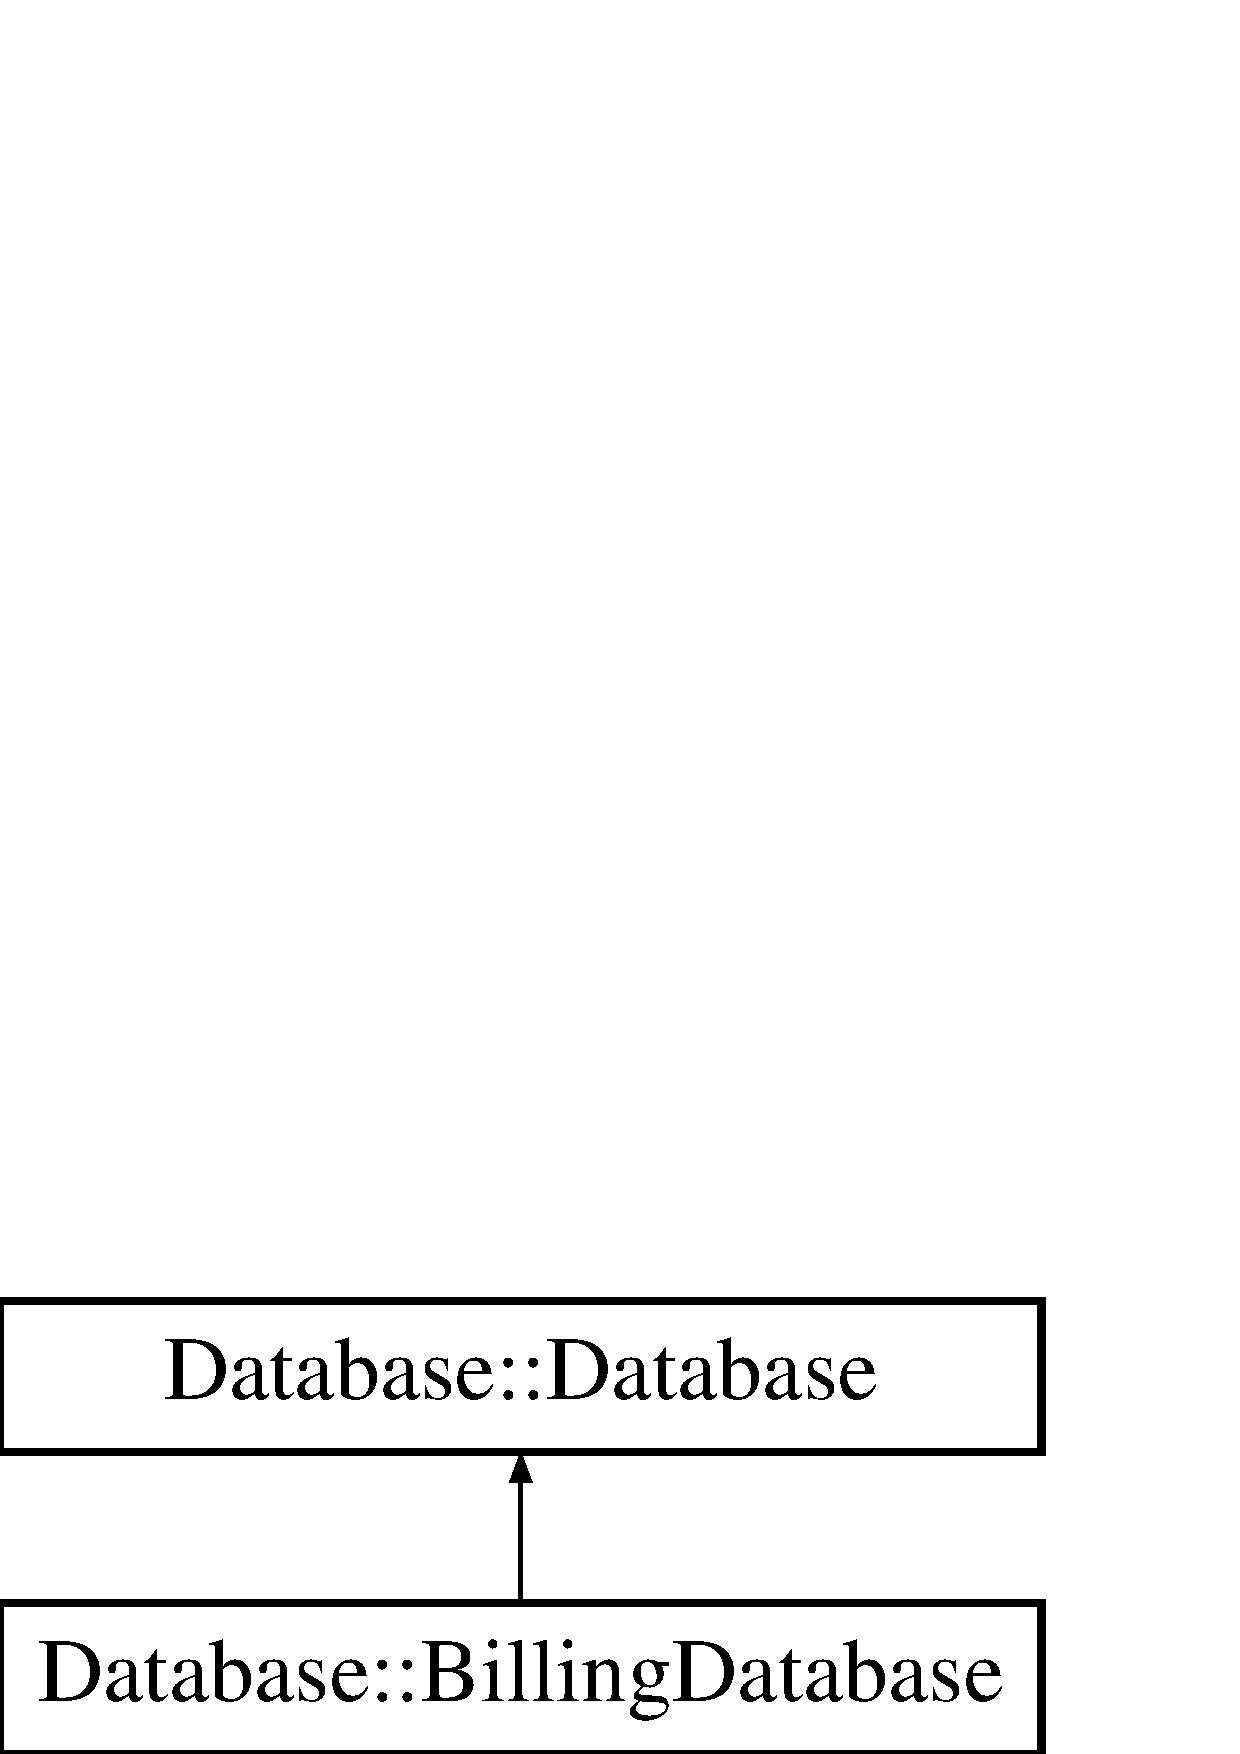
\includegraphics[height=2.000000cm]{d2/d86/classDatabase_1_1BillingDatabase}
\end{center}
\end{figure}
\subsection*{Public Member Functions}
\begin{DoxyCompactItemize}
\item 
\hyperlink{classModels_1_1Billing}{Models\+::\+Billing} $\ast$ \hyperlink{classDatabase_1_1BillingDatabase_a3063746cff15d93c4f5f319d53381579}{get\+Billing} (const int p\+Id)
\begin{DoxyCompactList}\small\item\em Billing\+Database\+::get\+Customer get informations about the billing identified by {\itshape p\+Id} \end{DoxyCompactList}\item 
Q\+Standard\+Item\+Model $\ast$ \hyperlink{classDatabase_1_1BillingDatabase_a3d3aec676ed5f7862197cac63adb18e9}{get\+Billings\+Table} (const int id\+Project)  throw (\+Db\+Exception$\ast$)
\begin{DoxyCompactList}\small\item\em \hyperlink{classDatabase_1_1BillingDatabase_a3d3aec676ed5f7862197cac63adb18e9}{Billing\+Database\+::get\+Billings\+Table} Return an item model of billings for Q\+Table\+View. \end{DoxyCompactList}\item 
int \hyperlink{classDatabase_1_1BillingDatabase_aa08b3b4917eb6c447ef513e5aafff38f}{add\+Billing} (const \hyperlink{classModels_1_1Billing}{Models\+::\+Billing} \&)
\begin{DoxyCompactList}\small\item\em \hyperlink{classDatabase_1_1BillingDatabase_aa08b3b4917eb6c447ef513e5aafff38f}{Billing\+Database\+::add\+Billing} Add the billing {\itshape p\+Billing} to the database. \end{DoxyCompactList}\item 
\hypertarget{classDatabase_1_1BillingDatabase_a59830561e9573ab3ce463e9dc1b68a0c}{void \hyperlink{classDatabase_1_1BillingDatabase_a59830561e9573ab3ce463e9dc1b68a0c}{update\+Billing} (const \hyperlink{classModels_1_1Billing}{Models\+::\+Billing} \&)}\label{classDatabase_1_1BillingDatabase_a59830561e9573ab3ce463e9dc1b68a0c}

\begin{DoxyCompactList}\small\item\em Billing\+Database\+::update\+Customer Update informations about the billing {\itshape p\+Customer} \end{DoxyCompactList}\item 
void \hyperlink{classDatabase_1_1BillingDatabase_af419d6b120523e9c67d5c89bcfcd44dd}{remove\+Billing} (const int p\+Id)
\begin{DoxyCompactList}\small\item\em Billing\+Database\+::remove\+Customer Remove the billing with the id {\itshape p\+Id} \end{DoxyCompactList}\item 
void \hyperlink{classDatabase_1_1BillingDatabase_a38514a0874d27551c67d56b9a7ec340e}{add\+Billing\+Project} (const int id\+Project, const int id\+Billing, const int id\+Contributory)
\begin{DoxyCompactList}\small\item\em \hyperlink{classDatabase_1_1BillingDatabase_a38514a0874d27551c67d56b9a7ec340e}{Billing\+Database\+::add\+Billing\+Project} Link a project, a billing and a contributory in the table Billing\+Project. \end{DoxyCompactList}\item 
int \hyperlink{classDatabase_1_1BillingDatabase_ac00c08641d0f4cc0596430f8e888ee38}{get\+Max\+Billing\+Number} ()
\begin{DoxyCompactList}\small\item\em get\+Max\+Billing\+Number Get the last number of a billing \end{DoxyCompactList}\item 
int \hyperlink{classDatabase_1_1BillingDatabase_ad9fe39d053a7f8686e1d94bc41eda03e}{get\+Max\+Quote\+Nuber} ()
\begin{DoxyCompactList}\small\item\em get\+Max\+Quote\+Nuber Get the last number of a quote \end{DoxyCompactList}\end{DoxyCompactItemize}
\subsection*{Static Public Member Functions}
\begin{DoxyCompactItemize}
\item 
static \hyperlink{classDatabase_1_1BillingDatabase}{Billing\+Database} $\ast$ \hyperlink{classDatabase_1_1BillingDatabase_a3ab4bd6cc25a186856aac757d6213aa0}{instance} ()  throw (\+Db\+Exception$\ast$)
\begin{DoxyCompactList}\small\item\em Billing\+Database\+::get\+Instance Return an instance of {\bfseries \hyperlink{classDatabase_1_1BillingDatabase}{Billing\+Database}} \end{DoxyCompactList}\end{DoxyCompactItemize}
\subsection*{Additional Inherited Members}


\subsection{Detailed Description}
The {\bfseries \hyperlink{classDatabase_1_1BillingDatabase}{Billing\+Database}} class Billing (or Quote) table database. 

\begin{DoxyAuthor}{Author}
Cédric Rohaut  
\end{DoxyAuthor}
\begin{DoxySeeAlso}{See also}
\hyperlink{classDatabase_1_1Database}{Database} 

Billing/\+Quote 
\end{DoxySeeAlso}


\subsection{Member Function Documentation}
\hypertarget{classDatabase_1_1BillingDatabase_aa08b3b4917eb6c447ef513e5aafff38f}{\index{Database\+::\+Billing\+Database@{Database\+::\+Billing\+Database}!add\+Billing@{add\+Billing}}
\index{add\+Billing@{add\+Billing}!Database\+::\+Billing\+Database@{Database\+::\+Billing\+Database}}
\subsubsection[{add\+Billing}]{\setlength{\rightskip}{0pt plus 5cm}int Database\+::\+Billing\+Database\+::add\+Billing (
\begin{DoxyParamCaption}
\item[{const {\bf Models\+::\+Billing} \&}]{p\+Billing}
\end{DoxyParamCaption}
)}}\label{classDatabase_1_1BillingDatabase_aa08b3b4917eb6c447ef513e5aafff38f}


\hyperlink{classDatabase_1_1BillingDatabase_aa08b3b4917eb6c447ef513e5aafff38f}{Billing\+Database\+::add\+Billing} Add the billing {\itshape p\+Billing} to the database. 

\begin{DoxyReturn}{Returns}
billing id 
\end{DoxyReturn}
\hypertarget{classDatabase_1_1BillingDatabase_a38514a0874d27551c67d56b9a7ec340e}{\index{Database\+::\+Billing\+Database@{Database\+::\+Billing\+Database}!add\+Billing\+Project@{add\+Billing\+Project}}
\index{add\+Billing\+Project@{add\+Billing\+Project}!Database\+::\+Billing\+Database@{Database\+::\+Billing\+Database}}
\subsubsection[{add\+Billing\+Project}]{\setlength{\rightskip}{0pt plus 5cm}void Database\+::\+Billing\+Database\+::add\+Billing\+Project (
\begin{DoxyParamCaption}
\item[{const int}]{id\+Project, }
\item[{const int}]{id\+Billing, }
\item[{const int}]{id\+Contributory}
\end{DoxyParamCaption}
)}}\label{classDatabase_1_1BillingDatabase_a38514a0874d27551c67d56b9a7ec340e}


\hyperlink{classDatabase_1_1BillingDatabase_a38514a0874d27551c67d56b9a7ec340e}{Billing\+Database\+::add\+Billing\+Project} Link a project, a billing and a contributory in the table Billing\+Project. 


\begin{DoxyParams}{Parameters}
{\em id\+Project} & Project id \\
\hline
{\em id\+Billing} & Billing id \\
\hline
{\em id\+Contributory} & Contributory id \\
\hline
\end{DoxyParams}
\hypertarget{classDatabase_1_1BillingDatabase_a3063746cff15d93c4f5f319d53381579}{\index{Database\+::\+Billing\+Database@{Database\+::\+Billing\+Database}!get\+Billing@{get\+Billing}}
\index{get\+Billing@{get\+Billing}!Database\+::\+Billing\+Database@{Database\+::\+Billing\+Database}}
\subsubsection[{get\+Billing}]{\setlength{\rightskip}{0pt plus 5cm}{\bf Models\+::\+Billing} $\ast$ Database\+::\+Billing\+Database\+::get\+Billing (
\begin{DoxyParamCaption}
\item[{const int}]{p\+Id}
\end{DoxyParamCaption}
)}}\label{classDatabase_1_1BillingDatabase_a3063746cff15d93c4f5f319d53381579}


Billing\+Database\+::get\+Customer get informations about the billing identified by {\itshape p\+Id} 


\begin{DoxyParams}{Parameters}
{\em p\+Id} & billing id \\
\hline
\end{DoxyParams}
\begin{DoxyReturn}{Returns}
the Billing 
\end{DoxyReturn}
\hypertarget{classDatabase_1_1BillingDatabase_a3d3aec676ed5f7862197cac63adb18e9}{\index{Database\+::\+Billing\+Database@{Database\+::\+Billing\+Database}!get\+Billings\+Table@{get\+Billings\+Table}}
\index{get\+Billings\+Table@{get\+Billings\+Table}!Database\+::\+Billing\+Database@{Database\+::\+Billing\+Database}}
\subsubsection[{get\+Billings\+Table}]{\setlength{\rightskip}{0pt plus 5cm}Q\+Standard\+Item\+Model $\ast$ Database\+::\+Billing\+Database\+::get\+Billings\+Table (
\begin{DoxyParamCaption}
\item[{const int}]{id\+Project}
\end{DoxyParamCaption}
) throw  {\bf Db\+Exception} $\ast$) }}\label{classDatabase_1_1BillingDatabase_a3d3aec676ed5f7862197cac63adb18e9}


\hyperlink{classDatabase_1_1BillingDatabase_a3d3aec676ed5f7862197cac63adb18e9}{Billing\+Database\+::get\+Billings\+Table} Return an item model of billings for Q\+Table\+View. 


\begin{DoxyParams}{Parameters}
{\em p\+Id} & the project id of the billings returned \\
\hline
\end{DoxyParams}

\begin{DoxyExceptions}{Exceptions}
{\em Db\+Exception} & \\
\hline
\end{DoxyExceptions}
\begin{DoxyReturn}{Returns}
Q\+Standard\+Item\+Model an item model for Q\+Table\+View 
\end{DoxyReturn}
\hypertarget{classDatabase_1_1BillingDatabase_ac00c08641d0f4cc0596430f8e888ee38}{\index{Database\+::\+Billing\+Database@{Database\+::\+Billing\+Database}!get\+Max\+Billing\+Number@{get\+Max\+Billing\+Number}}
\index{get\+Max\+Billing\+Number@{get\+Max\+Billing\+Number}!Database\+::\+Billing\+Database@{Database\+::\+Billing\+Database}}
\subsubsection[{get\+Max\+Billing\+Number}]{\setlength{\rightskip}{0pt plus 5cm}int Database\+::\+Billing\+Database\+::get\+Max\+Billing\+Number (
\begin{DoxyParamCaption}
{}
\end{DoxyParamCaption}
)}}\label{classDatabase_1_1BillingDatabase_ac00c08641d0f4cc0596430f8e888ee38}


get\+Max\+Billing\+Number Get the last number of a billing 

\begin{DoxyReturn}{Returns}
The max number 
\end{DoxyReturn}
\hypertarget{classDatabase_1_1BillingDatabase_ad9fe39d053a7f8686e1d94bc41eda03e}{\index{Database\+::\+Billing\+Database@{Database\+::\+Billing\+Database}!get\+Max\+Quote\+Nuber@{get\+Max\+Quote\+Nuber}}
\index{get\+Max\+Quote\+Nuber@{get\+Max\+Quote\+Nuber}!Database\+::\+Billing\+Database@{Database\+::\+Billing\+Database}}
\subsubsection[{get\+Max\+Quote\+Nuber}]{\setlength{\rightskip}{0pt plus 5cm}int Database\+::\+Billing\+Database\+::get\+Max\+Quote\+Nuber (
\begin{DoxyParamCaption}
{}
\end{DoxyParamCaption}
)}}\label{classDatabase_1_1BillingDatabase_ad9fe39d053a7f8686e1d94bc41eda03e}


get\+Max\+Quote\+Nuber Get the last number of a quote 

\begin{DoxyReturn}{Returns}
The last number 
\end{DoxyReturn}
\hypertarget{classDatabase_1_1BillingDatabase_a3ab4bd6cc25a186856aac757d6213aa0}{\index{Database\+::\+Billing\+Database@{Database\+::\+Billing\+Database}!instance@{instance}}
\index{instance@{instance}!Database\+::\+Billing\+Database@{Database\+::\+Billing\+Database}}
\subsubsection[{instance}]{\setlength{\rightskip}{0pt plus 5cm}{\bf Billing\+Database} $\ast$ Database\+::\+Billing\+Database\+::instance (
\begin{DoxyParamCaption}
{}
\end{DoxyParamCaption}
) throw  {\bf Db\+Exception} $\ast$) \hspace{0.3cm}{\ttfamily [static]}}}\label{classDatabase_1_1BillingDatabase_a3ab4bd6cc25a186856aac757d6213aa0}


Billing\+Database\+::get\+Instance Return an instance of {\bfseries \hyperlink{classDatabase_1_1BillingDatabase}{Billing\+Database}} 

\begin{DoxySeeAlso}{See also}
Db\+Exception 
\end{DoxySeeAlso}
\begin{DoxyReturn}{Returns}
Instance of \hyperlink{classDatabase_1_1BillingDatabase}{Billing\+Database} 
\end{DoxyReturn}
\hypertarget{classDatabase_1_1BillingDatabase_af419d6b120523e9c67d5c89bcfcd44dd}{\index{Database\+::\+Billing\+Database@{Database\+::\+Billing\+Database}!remove\+Billing@{remove\+Billing}}
\index{remove\+Billing@{remove\+Billing}!Database\+::\+Billing\+Database@{Database\+::\+Billing\+Database}}
\subsubsection[{remove\+Billing}]{\setlength{\rightskip}{0pt plus 5cm}void Database\+::\+Billing\+Database\+::remove\+Billing (
\begin{DoxyParamCaption}
\item[{const int}]{p\+Id}
\end{DoxyParamCaption}
)}}\label{classDatabase_1_1BillingDatabase_af419d6b120523e9c67d5c89bcfcd44dd}


Billing\+Database\+::remove\+Customer Remove the billing with the id {\itshape p\+Id} 


\begin{DoxyParams}{Parameters}
{\em p\+Id} & billing id \\
\hline
\end{DoxyParams}


The documentation for this class was generated from the following files\+:\begin{DoxyCompactItemize}
\item 
src/database/billingdatabase.\+h\item 
src/database/billingdatabase.\+cpp\end{DoxyCompactItemize}

\hypertarget{classBillingDatabaseTest}{\section{Billing\+Database\+Test Class Reference}
\label{classBillingDatabaseTest}\index{Billing\+Database\+Test@{Billing\+Database\+Test}}
}
Inheritance diagram for Billing\+Database\+Test\+:\begin{figure}[H]
\begin{center}
\leavevmode
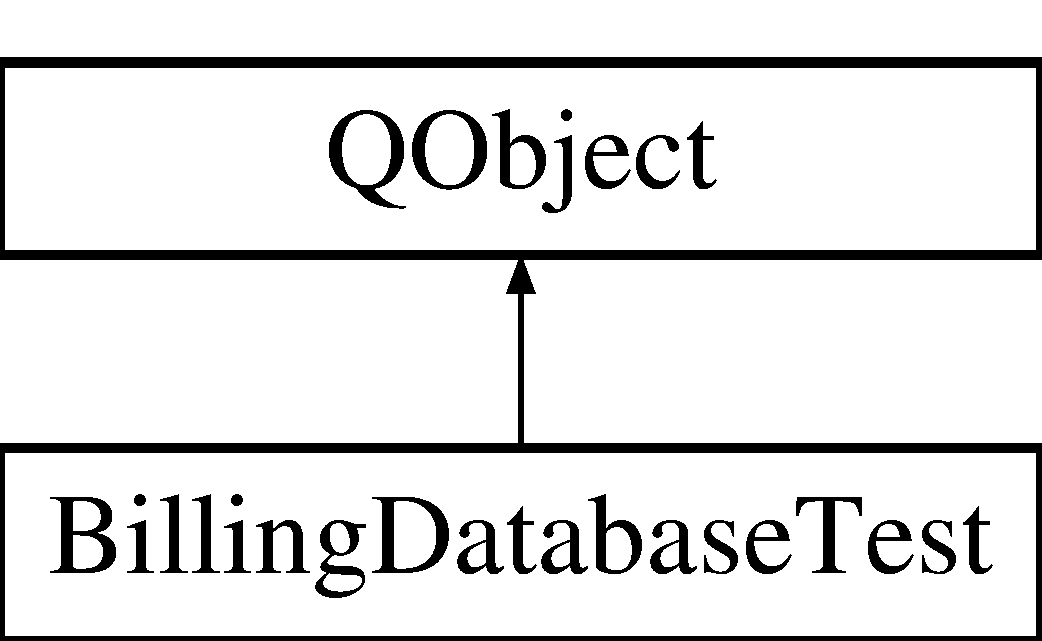
\includegraphics[height=2.000000cm]{d1/db1/classBillingDatabaseTest}
\end{center}
\end{figure}


The documentation for this class was generated from the following files\+:\begin{DoxyCompactItemize}
\item 
tests/database/billingdatabasetest.\+h\item 
tests/database/billingdatabasetest.\+cpp\end{DoxyCompactItemize}

\hypertarget{classBillingModelTest}{\section{Billing\-Model\-Test Class Reference}
\label{classBillingModelTest}\index{Billing\-Model\-Test@{Billing\-Model\-Test}}
}
Inheritance diagram for Billing\-Model\-Test\-:\begin{figure}[H]
\begin{center}
\leavevmode
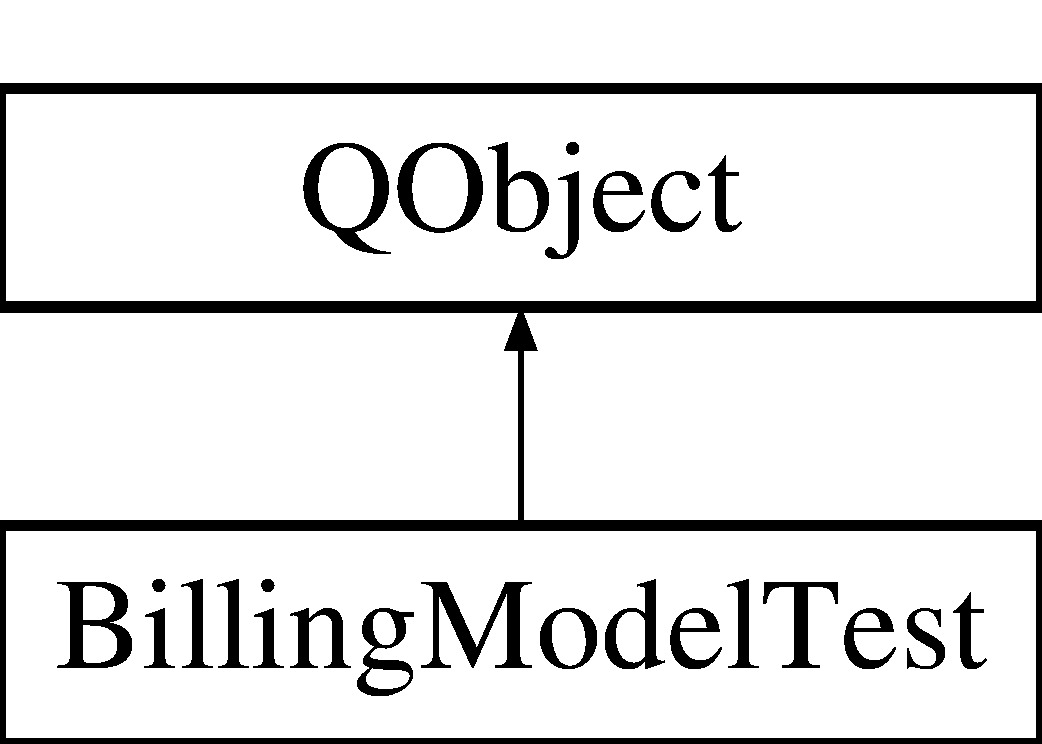
\includegraphics[height=2.000000cm]{dc/d0c/classBillingModelTest}
\end{center}
\end{figure}


The documentation for this class was generated from the following files\-:\begin{DoxyCompactItemize}
\item 
/home/florent/\-Documents/\-Projet\-\_\-\-S8/\-Fact\-Dev/tests/models/billingmodeltest.\-h\item 
/home/florent/\-Documents/\-Projet\-\_\-\-S8/\-Fact\-Dev/tests/models/billingmodeltest.\-cpp\end{DoxyCompactItemize}

\hypertarget{classCheckCity}{\section{Check\+City Class Reference}
\label{classCheckCity}\index{Check\+City@{Check\+City}}
}


The \hyperlink{classCheckCity}{Check\+City} class Line Edit of City with a check icon.  




{\ttfamily \#include $<$checkcity.\+h$>$}

Inheritance diagram for Check\+City\+:\begin{figure}[H]
\begin{center}
\leavevmode
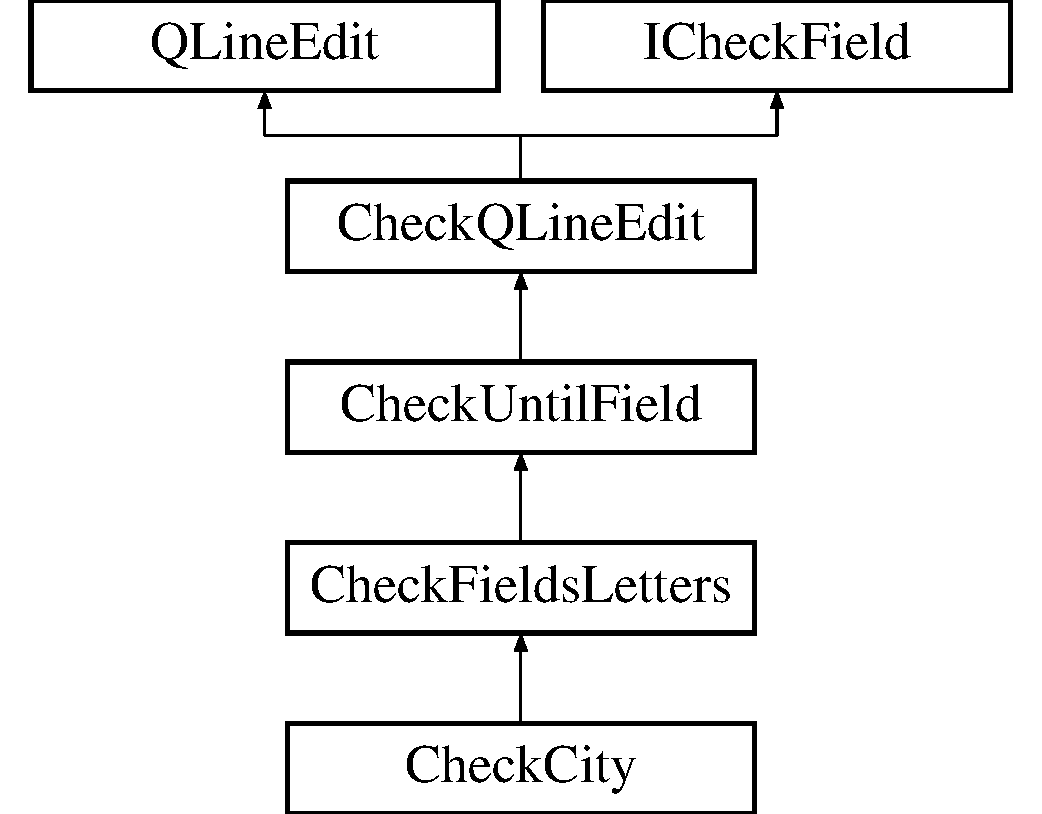
\includegraphics[height=5.000000cm]{de/de9/classCheckCity}
\end{center}
\end{figure}
\subsection*{Public Member Functions}
\begin{DoxyCompactItemize}
\item 
\hyperlink{classCheckCity_a639556875bd01b8cee5cf92759972ca5}{Check\+City} (Q\+Widget $\ast$w=0, Q\+Push\+Button $\ast$btn=0)
\begin{DoxyCompactList}\small\item\em \hyperlink{classCheckCity_a639556875bd01b8cee5cf92759972ca5}{Check\+City\+::\+Check\+City} Construct a \hyperlink{classCheckCity}{Check\+City}. \end{DoxyCompactList}\end{DoxyCompactItemize}
\subsection*{Additional Inherited Members}


\subsection{Detailed Description}
The \hyperlink{classCheckCity}{Check\+City} class Line Edit of City with a check icon. 

\subsection{Constructor \& Destructor Documentation}
\hypertarget{classCheckCity_a639556875bd01b8cee5cf92759972ca5}{\index{Check\+City@{Check\+City}!Check\+City@{Check\+City}}
\index{Check\+City@{Check\+City}!Check\+City@{Check\+City}}
\subsubsection[{Check\+City}]{\setlength{\rightskip}{0pt plus 5cm}Check\+City\+::\+Check\+City (
\begin{DoxyParamCaption}
\item[{Q\+Widget $\ast$}]{w = {\ttfamily 0}, }
\item[{Q\+Push\+Button $\ast$}]{btn = {\ttfamily 0}}
\end{DoxyParamCaption}
)}}\label{classCheckCity_a639556875bd01b8cee5cf92759972ca5}


\hyperlink{classCheckCity_a639556875bd01b8cee5cf92759972ca5}{Check\+City\+::\+Check\+City} Construct a \hyperlink{classCheckCity}{Check\+City}. 


\begin{DoxyParams}{Parameters}
{\em w} & Q\+Widget linked to {\bfseries \hyperlink{classCheckCity}{Check\+City}} \\
\hline
\end{DoxyParams}


The documentation for this class was generated from the following files\+:\begin{DoxyCompactItemize}
\item 
src/gui/widgets/checkfields/checkcity.\+h\item 
src/gui/widgets/checkfields/checkcity.\+cpp\end{DoxyCompactItemize}

\hypertarget{classCheckCountry}{\section{Check\-Country Class Reference}
\label{classCheckCountry}\index{Check\-Country@{Check\-Country}}
}


\hyperlink{classCheckCountry_aa6aa76f22635d879105449836dd68bbd}{Check\-Country\-::\-Check\-Country} Line Edit of country with a check icon.  




{\ttfamily \#include $<$checkcountry.\-h$>$}

Inheritance diagram for Check\-Country\-:\begin{figure}[H]
\begin{center}
\leavevmode
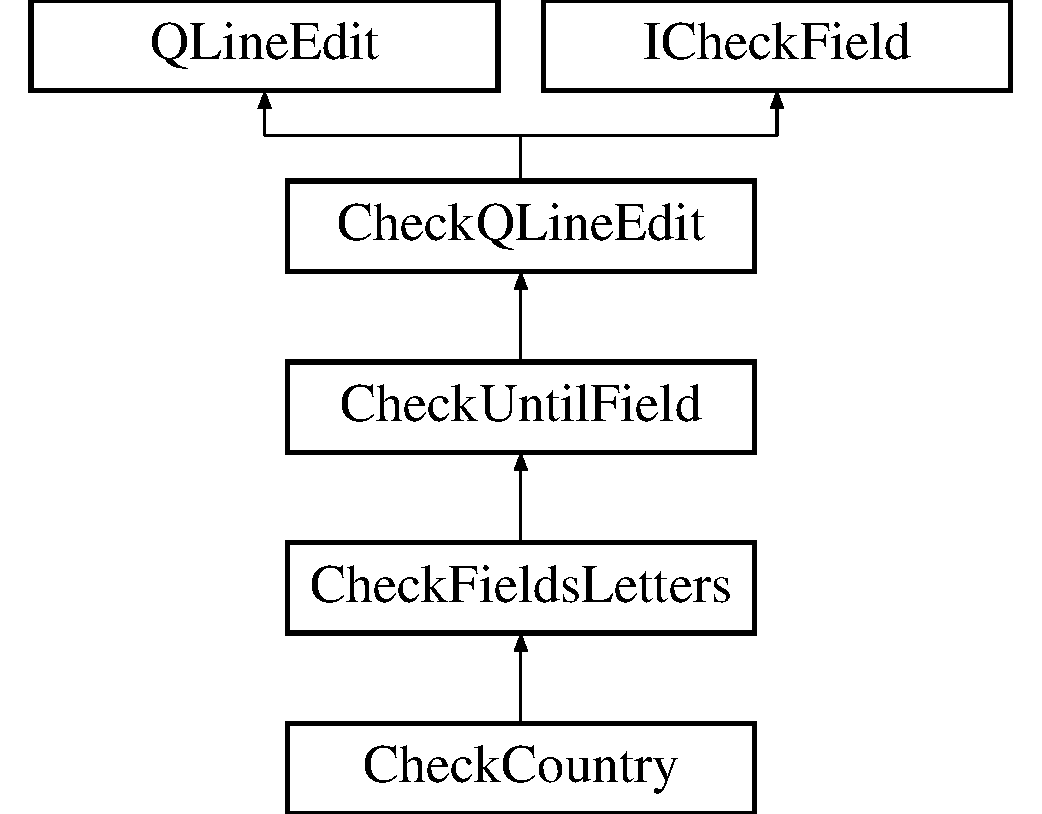
\includegraphics[height=5.000000cm]{d6/d52/classCheckCountry}
\end{center}
\end{figure}
\subsection*{Public Member Functions}
\begin{DoxyCompactItemize}
\item 
\hyperlink{classCheckCountry_aa6aa76f22635d879105449836dd68bbd}{Check\-Country} (Q\-Widget $\ast$w=0, Q\-Push\-Button $\ast$btn=0)
\begin{DoxyCompactList}\small\item\em Check\-Email\-::\-Check\-Country Construct a \hyperlink{classCheckCountry}{Check\-Country}. \end{DoxyCompactList}\end{DoxyCompactItemize}
\subsection*{Additional Inherited Members}


\subsection{Detailed Description}
\hyperlink{classCheckCountry_aa6aa76f22635d879105449836dd68bbd}{Check\-Country\-::\-Check\-Country} Line Edit of country with a check icon. 

\subsection{Constructor \& Destructor Documentation}
\hypertarget{classCheckCountry_aa6aa76f22635d879105449836dd68bbd}{\index{Check\-Country@{Check\-Country}!Check\-Country@{Check\-Country}}
\index{Check\-Country@{Check\-Country}!CheckCountry@{Check\-Country}}
\subsubsection[{Check\-Country}]{\setlength{\rightskip}{0pt plus 5cm}Check\-Country\-::\-Check\-Country (
\begin{DoxyParamCaption}
\item[{Q\-Widget $\ast$}]{w = {\ttfamily 0}, }
\item[{Q\-Push\-Button $\ast$}]{btn = {\ttfamily 0}}
\end{DoxyParamCaption}
)}}\label{classCheckCountry_aa6aa76f22635d879105449836dd68bbd}


Check\-Email\-::\-Check\-Country Construct a \hyperlink{classCheckCountry}{Check\-Country}. 


\begin{DoxyParams}{Parameters}
{\em w} & Q\-Widget linked to {\bfseries \hyperlink{classCheckCountry}{Check\-Country}} \\
\hline
\end{DoxyParams}


The documentation for this class was generated from the following files\-:\begin{DoxyCompactItemize}
\item 
/home/florent/\-Documents/\-Projet\-\_\-\-S8/\-Fact\-Dev/src/gui/widgets/checkfields/checkcountry.\-h\item 
/home/florent/\-Documents/\-Projet\-\_\-\-S8/\-Fact\-Dev/src/gui/widgets/checkfields/checkcountry.\-cpp\end{DoxyCompactItemize}

\hypertarget{classCheckEmail}{\section{Check\-Email Class Reference}
\label{classCheckEmail}\index{Check\-Email@{Check\-Email}}
}


The \hyperlink{classCheckEmail}{Check\-Email} class Line Edit of email with a check icon.  




{\ttfamily \#include $<$checkemail.\-h$>$}

Inheritance diagram for Check\-Email\-:\begin{figure}[H]
\begin{center}
\leavevmode
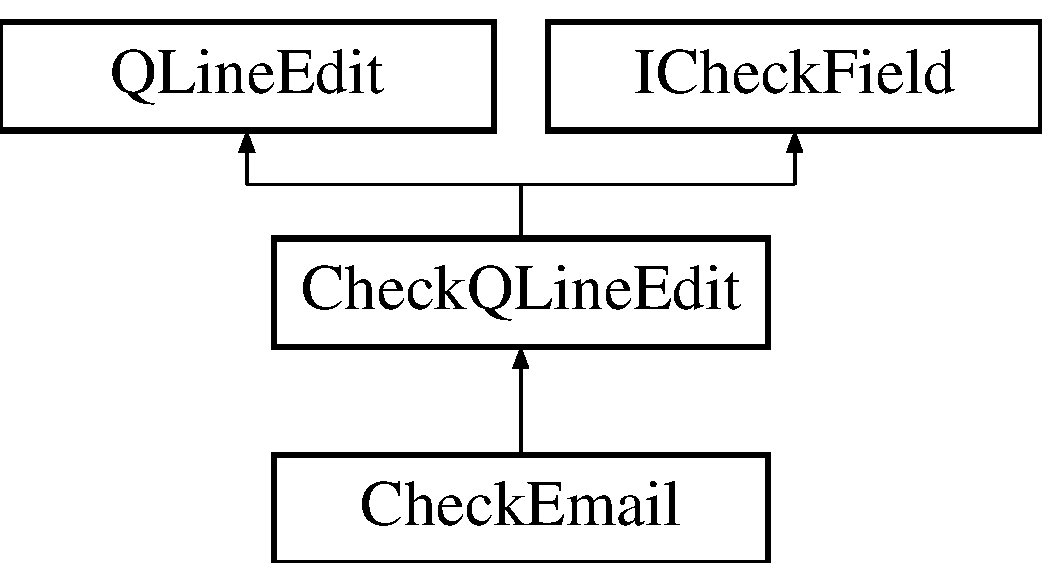
\includegraphics[height=3.000000cm]{da/d1d/classCheckEmail}
\end{center}
\end{figure}
\subsection*{Public Member Functions}
\begin{DoxyCompactItemize}
\item 
\hyperlink{classCheckEmail_a385bd05063deaf42fc02918b9348c8ac}{Check\-Email} (Q\-Widget $\ast$w=0, Q\-Push\-Button $\ast$btn=0)
\begin{DoxyCompactList}\small\item\em \hyperlink{classCheckEmail_a385bd05063deaf42fc02918b9348c8ac}{Check\-Email\-::\-Check\-Email} Construct a Check\-Mail. \end{DoxyCompactList}\item 
bool \hyperlink{classCheckEmail_a544d7656d36bd463391fe2f4dd3e13c6}{check} (const Q\-String text)
\begin{DoxyCompactList}\small\item\em \hyperlink{classCheckEmail_a544d7656d36bd463391fe2f4dd3e13c6}{Check\-Email\-::check} Check if the field email is valid. To be valid, an email address should be under this form\-: \href{mailto:me@me.xx}{\tt me@me.\-xx} An email address need\-: \end{DoxyCompactList}\end{DoxyCompactItemize}
\subsection*{Additional Inherited Members}


\subsection{Detailed Description}
The \hyperlink{classCheckEmail}{Check\-Email} class Line Edit of email with a check icon. 

\subsection{Constructor \& Destructor Documentation}
\hypertarget{classCheckEmail_a385bd05063deaf42fc02918b9348c8ac}{\index{Check\-Email@{Check\-Email}!Check\-Email@{Check\-Email}}
\index{Check\-Email@{Check\-Email}!CheckEmail@{Check\-Email}}
\subsubsection[{Check\-Email}]{\setlength{\rightskip}{0pt plus 5cm}Check\-Email\-::\-Check\-Email (
\begin{DoxyParamCaption}
\item[{Q\-Widget $\ast$}]{w = {\ttfamily 0}, }
\item[{Q\-Push\-Button $\ast$}]{btn = {\ttfamily 0}}
\end{DoxyParamCaption}
)}}\label{classCheckEmail_a385bd05063deaf42fc02918b9348c8ac}


\hyperlink{classCheckEmail_a385bd05063deaf42fc02918b9348c8ac}{Check\-Email\-::\-Check\-Email} Construct a Check\-Mail. 


\begin{DoxyParams}{Parameters}
{\em w} & Q\-Widget linked to {\bfseries \hyperlink{classCheckEmail}{Check\-Email}} \\
\hline
\end{DoxyParams}


\subsection{Member Function Documentation}
\hypertarget{classCheckEmail_a544d7656d36bd463391fe2f4dd3e13c6}{\index{Check\-Email@{Check\-Email}!check@{check}}
\index{check@{check}!CheckEmail@{Check\-Email}}
\subsubsection[{check}]{\setlength{\rightskip}{0pt plus 5cm}bool Check\-Email\-::check (
\begin{DoxyParamCaption}
\item[{const Q\-String}]{text}
\end{DoxyParamCaption}
)\hspace{0.3cm}{\ttfamily [virtual]}}}\label{classCheckEmail_a544d7656d36bd463391fe2f4dd3e13c6}


\hyperlink{classCheckEmail_a544d7656d36bd463391fe2f4dd3e13c6}{Check\-Email\-::check} Check if the field email is valid. To be valid, an email address should be under this form\-: \href{mailto:me@me.xx}{\tt me@me.\-xx} An email address need\-: 


\begin{DoxyItemize}
\item 1 character \mbox{[}A-\/\-Z\mbox{]} or \mbox{[}a-\/z\mbox{]} minimum before the character {\itshape $<$/i$>$}
\item {\itshape the character '@'}
\item {\itshape 1 character \mbox{[}A-\/\-Z\mbox{]} or \mbox{[}a-\/z\mbox{]} after the character{\itshape $<$/i$>$minimum and before the character {\itshape .}}}
\item {\itshape {\itshape 1 character \mbox{[}A-\/\-Z\mbox{]} or \mbox{[}a-\/z\mbox{]} minimum afer the character {\itshape .} Return T\-R\-U\-E if email address is valid, else F\-A\-L\-S\-E 
\begin{DoxyParams}{Parameters}
{\em text} & \\
\hline
\end{DoxyParams}
\begin{DoxyReturn}{Returns}
boolean 
\end{DoxyReturn}
}}
\end{DoxyItemize}

Implements \hyperlink{classICheckField_a6bd42b4d49c165cdd92822135123fd4b}{I\-Check\-Field}.



The documentation for this class was generated from the following files\-:\begin{DoxyCompactItemize}
\item 
/home/florent/\-Documents/\-Projet\-\_\-\-S8/\-Fact\-Dev/src/gui/widgets/checkfields/checkemail.\-h\item 
/home/florent/\-Documents/\-Projet\-\_\-\-S8/\-Fact\-Dev/src/gui/widgets/checkfields/checkemail.\-cpp\end{DoxyCompactItemize}

\hypertarget{classCheckFieldsLetters}{\section{Check\-Fields\-Letters Class Reference}
\label{classCheckFieldsLetters}\index{Check\-Fields\-Letters@{Check\-Fields\-Letters}}
}


The \hyperlink{classCheckFieldsLetters}{Check\-Fields\-Letters} class Field with only letters (no numbers)  




{\ttfamily \#include $<$checkfieldsletters.\-h$>$}

Inheritance diagram for Check\-Fields\-Letters\-:\begin{figure}[H]
\begin{center}
\leavevmode
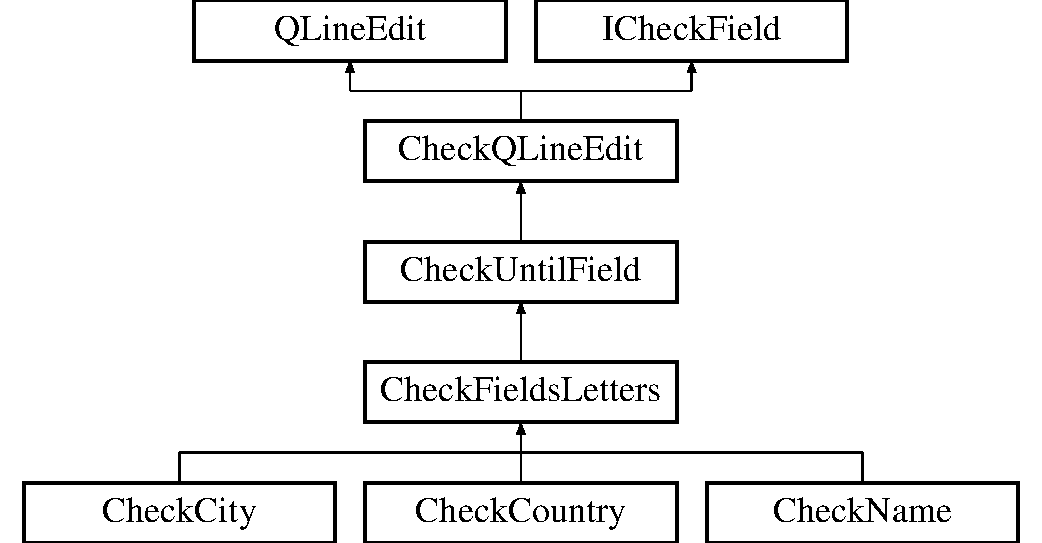
\includegraphics[height=5.000000cm]{de/d19/classCheckFieldsLetters}
\end{center}
\end{figure}
\subsection*{Public Member Functions}
\begin{DoxyCompactItemize}
\item 
\hyperlink{classCheckFieldsLetters_a5a8af8c6e89dc19c7e98304e5f40081d}{Check\-Fields\-Letters} (Q\-Widget $\ast$w=0, Q\-Push\-Button $\ast$btn=0)
\begin{DoxyCompactList}\small\item\em \hyperlink{classCheckFieldsLetters_a5a8af8c6e89dc19c7e98304e5f40081d}{Check\-Fields\-Letters\-::\-Check\-Fields\-Letters} Construct a \hyperlink{classCheckFieldsLetters}{Check\-Fields\-Letters}. \end{DoxyCompactList}\item 
bool \hyperlink{classCheckFieldsLetters_a62574deb407fe83456e46381425a7b46}{check} (Q\-String text)
\begin{DoxyCompactList}\small\item\em \hyperlink{classCheckFieldsLetters_a62574deb407fe83456e46381425a7b46}{Check\-Name\-::check} Check if the field contains only letters. \end{DoxyCompactList}\end{DoxyCompactItemize}
\subsection*{Additional Inherited Members}


\subsection{Detailed Description}
The \hyperlink{classCheckFieldsLetters}{Check\-Fields\-Letters} class Field with only letters (no numbers) 

\subsection{Constructor \& Destructor Documentation}
\hypertarget{classCheckFieldsLetters_a5a8af8c6e89dc19c7e98304e5f40081d}{\index{Check\-Fields\-Letters@{Check\-Fields\-Letters}!Check\-Fields\-Letters@{Check\-Fields\-Letters}}
\index{Check\-Fields\-Letters@{Check\-Fields\-Letters}!CheckFieldsLetters@{Check\-Fields\-Letters}}
\subsubsection[{Check\-Fields\-Letters}]{\setlength{\rightskip}{0pt plus 5cm}Check\-Fields\-Letters\-::\-Check\-Fields\-Letters (
\begin{DoxyParamCaption}
\item[{Q\-Widget $\ast$}]{w = {\ttfamily 0}, }
\item[{Q\-Push\-Button $\ast$}]{btn = {\ttfamily 0}}
\end{DoxyParamCaption}
)}}\label{classCheckFieldsLetters_a5a8af8c6e89dc19c7e98304e5f40081d}


\hyperlink{classCheckFieldsLetters_a5a8af8c6e89dc19c7e98304e5f40081d}{Check\-Fields\-Letters\-::\-Check\-Fields\-Letters} Construct a \hyperlink{classCheckFieldsLetters}{Check\-Fields\-Letters}. 


\begin{DoxyParams}{Parameters}
{\em w} & Q\-Widget linked to {\bfseries \hyperlink{classCheckFieldsLetters}{Check\-Fields\-Letters}} \\
\hline
\end{DoxyParams}


\subsection{Member Function Documentation}
\hypertarget{classCheckFieldsLetters_a62574deb407fe83456e46381425a7b46}{\index{Check\-Fields\-Letters@{Check\-Fields\-Letters}!check@{check}}
\index{check@{check}!CheckFieldsLetters@{Check\-Fields\-Letters}}
\subsubsection[{check}]{\setlength{\rightskip}{0pt plus 5cm}bool Check\-Fields\-Letters\-::check (
\begin{DoxyParamCaption}
\item[{Q\-String}]{text}
\end{DoxyParamCaption}
)\hspace{0.3cm}{\ttfamily [virtual]}}}\label{classCheckFieldsLetters_a62574deb407fe83456e46381425a7b46}


\hyperlink{classCheckFieldsLetters_a62574deb407fe83456e46381425a7b46}{Check\-Name\-::check} Check if the field contains only letters. 


\begin{DoxyParams}{Parameters}
{\em text} & \\
\hline
\end{DoxyParams}
\begin{DoxyReturn}{Returns}
boolean 
\end{DoxyReturn}


Implements \hyperlink{classICheckField_a6bd42b4d49c165cdd92822135123fd4b}{I\-Check\-Field}.



The documentation for this class was generated from the following files\-:\begin{DoxyCompactItemize}
\item 
/home/florent/\-Documents/\-Projet\-\_\-\-S8/\-Fact\-Dev/src/gui/widgets/checkfields/checkfieldsletters.\-h\item 
/home/florent/\-Documents/\-Projet\-\_\-\-S8/\-Fact\-Dev/src/gui/widgets/checkfields/checkfieldsletters.\-cpp\end{DoxyCompactItemize}

\hypertarget{classCheckName}{\section{Check\+Name Class Reference}
\label{classCheckName}\index{Check\+Name@{Check\+Name}}
}


The \hyperlink{classCheckName}{Check\+Name} class Line edit of name with a check icon.  




{\ttfamily \#include $<$checkname.\+h$>$}

Inheritance diagram for Check\+Name\+:\begin{figure}[H]
\begin{center}
\leavevmode
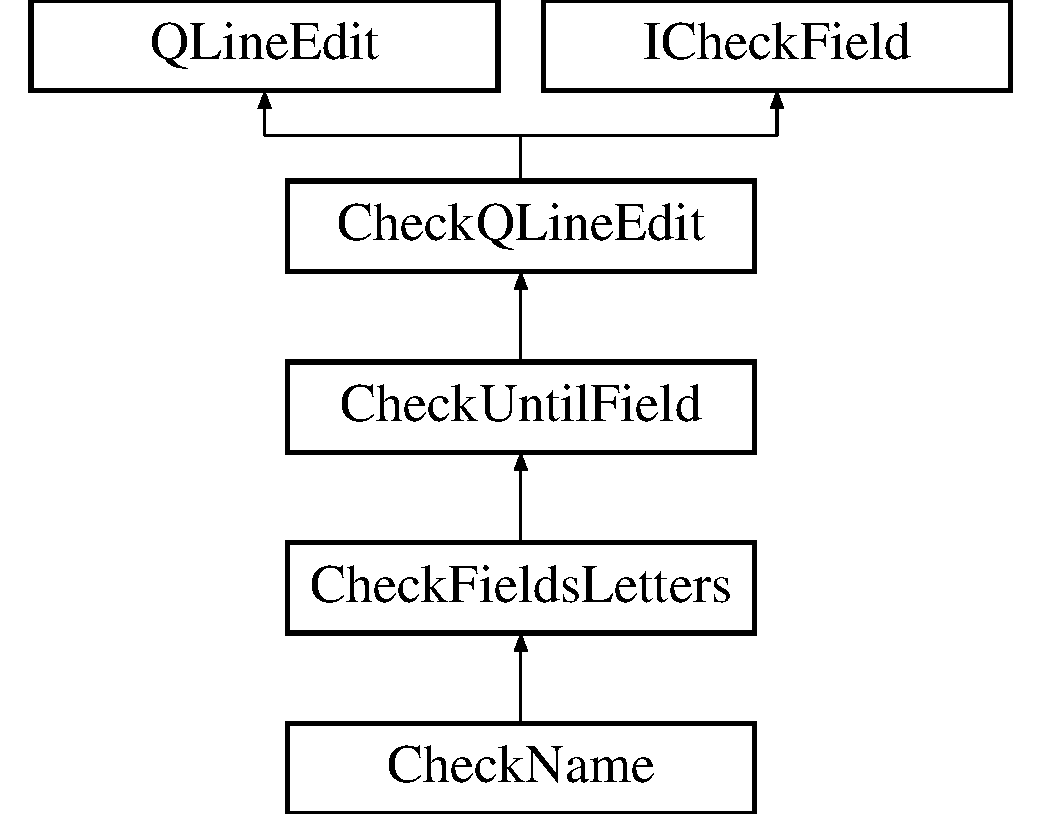
\includegraphics[height=5.000000cm]{dc/d14/classCheckName}
\end{center}
\end{figure}
\subsection*{Public Member Functions}
\begin{DoxyCompactItemize}
\item 
\hyperlink{classCheckName_a4a7fe601d6fd5e8576498e2d953df614}{Check\+Name} (Q\+Widget $\ast$w=0, Q\+Push\+Button $\ast$btn=0)
\begin{DoxyCompactList}\small\item\em \hyperlink{classCheckName_a4a7fe601d6fd5e8576498e2d953df614}{Check\+Name\+::\+Check\+Name} Construct a \hyperlink{classCheckName}{Check\+Name}. \end{DoxyCompactList}\end{DoxyCompactItemize}
\subsection*{Additional Inherited Members}


\subsection{Detailed Description}
The \hyperlink{classCheckName}{Check\+Name} class Line edit of name with a check icon. 

\subsection{Constructor \& Destructor Documentation}
\hypertarget{classCheckName_a4a7fe601d6fd5e8576498e2d953df614}{\index{Check\+Name@{Check\+Name}!Check\+Name@{Check\+Name}}
\index{Check\+Name@{Check\+Name}!Check\+Name@{Check\+Name}}
\subsubsection[{Check\+Name}]{\setlength{\rightskip}{0pt plus 5cm}Check\+Name\+::\+Check\+Name (
\begin{DoxyParamCaption}
\item[{Q\+Widget $\ast$}]{w = {\ttfamily 0}, }
\item[{Q\+Push\+Button $\ast$}]{btn = {\ttfamily 0}}
\end{DoxyParamCaption}
)}}\label{classCheckName_a4a7fe601d6fd5e8576498e2d953df614}


\hyperlink{classCheckName_a4a7fe601d6fd5e8576498e2d953df614}{Check\+Name\+::\+Check\+Name} Construct a \hyperlink{classCheckName}{Check\+Name}. 


\begin{DoxyParams}{Parameters}
{\em w} & Q\+Widget linked to {\bfseries \hyperlink{classCheckName}{Check\+Name}} \\
\hline
\end{DoxyParams}


The documentation for this class was generated from the following files\+:\begin{DoxyCompactItemize}
\item 
src/gui/widgets/checkfields/checkname.\+h\item 
src/gui/widgets/checkfields/checkname.\+cpp\end{DoxyCompactItemize}

\hypertarget{classCheckPhone}{\section{Check\+Phone Class Reference}
\label{classCheckPhone}\index{Check\+Phone@{Check\+Phone}}
}


The \hyperlink{classCheckPhone}{Check\+Phone} class Line Edit of Phone number with a check icon.  




{\ttfamily \#include $<$checkphone.\+h$>$}

Inheritance diagram for Check\+Phone\+:\begin{figure}[H]
\begin{center}
\leavevmode
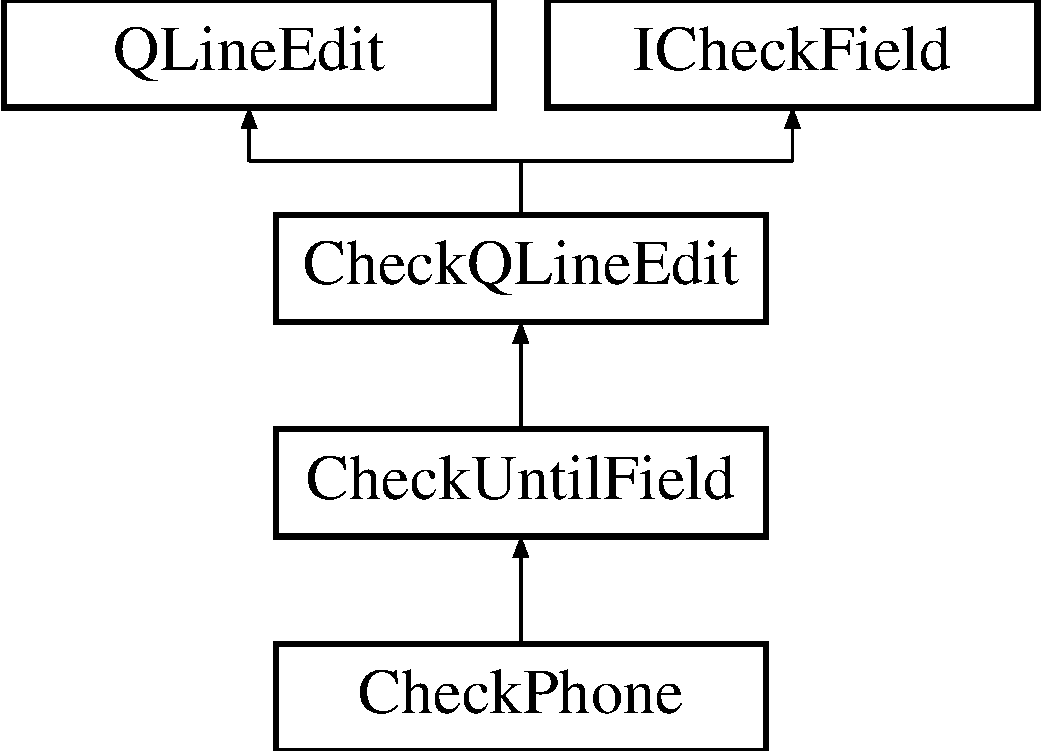
\includegraphics[height=4.000000cm]{d0/ddb/classCheckPhone}
\end{center}
\end{figure}
\subsection*{Public Member Functions}
\begin{DoxyCompactItemize}
\item 
\hyperlink{classCheckPhone_a491bceb9add48e7668162fc8ec511550}{Check\+Phone} (Q\+Widget $\ast$w=0, Q\+Push\+Button $\ast$btn=0)
\begin{DoxyCompactList}\small\item\em \hyperlink{classCheckPhone_a491bceb9add48e7668162fc8ec511550}{Check\+Phone\+::\+Check\+Phone} Construct a \hyperlink{classCheckPhone}{Check\+Phone}. \end{DoxyCompactList}\item 
bool \hyperlink{classCheckPhone_ac60f1428fc89e1b2630db022e14509ed}{check} (Q\+String text)
\begin{DoxyCompactList}\small\item\em \hyperlink{classCheckPhone_ac60f1428fc89e1b2630db022e14509ed}{Check\+Phone\+::check} Check if the field is valid. To be valid, a name should be composed of a character. \end{DoxyCompactList}\item 
Q\+String \hyperlink{classCheckPhone_a3dd528db0e731b23df0524e41415d05e}{get\+Country} () const 
\begin{DoxyCompactList}\small\item\em \hyperlink{classCheckPhone_a3dd528db0e731b23df0524e41415d05e}{Check\+Phone\+::get\+Country} Return the country linked to current field. \end{DoxyCompactList}\item 
void \hyperlink{classCheckPhone_a2a4a30d0a69611f72c539cc17919ccc9}{set\+Country} (const Q\+String \&country)
\begin{DoxyCompactList}\small\item\em \hyperlink{classCheckPhone_a2a4a30d0a69611f72c539cc17919ccc9}{Check\+Phone\+::set\+Country} Modify the {\itshape country} linked to field. \end{DoxyCompactList}\end{DoxyCompactItemize}
\subsection*{Additional Inherited Members}


\subsection{Detailed Description}
The \hyperlink{classCheckPhone}{Check\+Phone} class Line Edit of Phone number with a check icon. 

\subsection{Constructor \& Destructor Documentation}
\hypertarget{classCheckPhone_a491bceb9add48e7668162fc8ec511550}{\index{Check\+Phone@{Check\+Phone}!Check\+Phone@{Check\+Phone}}
\index{Check\+Phone@{Check\+Phone}!Check\+Phone@{Check\+Phone}}
\subsubsection[{Check\+Phone}]{\setlength{\rightskip}{0pt plus 5cm}Check\+Phone\+::\+Check\+Phone (
\begin{DoxyParamCaption}
\item[{Q\+Widget $\ast$}]{w = {\ttfamily 0}, }
\item[{Q\+Push\+Button $\ast$}]{btn = {\ttfamily 0}}
\end{DoxyParamCaption}
)}}\label{classCheckPhone_a491bceb9add48e7668162fc8ec511550}


\hyperlink{classCheckPhone_a491bceb9add48e7668162fc8ec511550}{Check\+Phone\+::\+Check\+Phone} Construct a \hyperlink{classCheckPhone}{Check\+Phone}. 


\begin{DoxyParams}{Parameters}
{\em w} & Q\+Widget linked to {\bfseries \hyperlink{classCheckPhone}{Check\+Phone}} \\
\hline
\end{DoxyParams}


\subsection{Member Function Documentation}
\hypertarget{classCheckPhone_ac60f1428fc89e1b2630db022e14509ed}{\index{Check\+Phone@{Check\+Phone}!check@{check}}
\index{check@{check}!Check\+Phone@{Check\+Phone}}
\subsubsection[{check}]{\setlength{\rightskip}{0pt plus 5cm}bool Check\+Phone\+::check (
\begin{DoxyParamCaption}
\item[{Q\+String}]{text}
\end{DoxyParamCaption}
)\hspace{0.3cm}{\ttfamily [virtual]}}}\label{classCheckPhone_ac60f1428fc89e1b2630db022e14509ed}


\hyperlink{classCheckPhone_ac60f1428fc89e1b2630db022e14509ed}{Check\+Phone\+::check} Check if the field is valid. To be valid, a name should be composed of a character. 


\begin{DoxyParams}{Parameters}
{\em text} & \\
\hline
\end{DoxyParams}
\begin{DoxyReturn}{Returns}
boolean 
\end{DoxyReturn}


Implements \hyperlink{classICheckField_a6bd42b4d49c165cdd92822135123fd4b}{I\+Check\+Field}.

\hypertarget{classCheckPhone_a3dd528db0e731b23df0524e41415d05e}{\index{Check\+Phone@{Check\+Phone}!get\+Country@{get\+Country}}
\index{get\+Country@{get\+Country}!Check\+Phone@{Check\+Phone}}
\subsubsection[{get\+Country}]{\setlength{\rightskip}{0pt plus 5cm}Q\+String Check\+Phone\+::get\+Country (
\begin{DoxyParamCaption}
{}
\end{DoxyParamCaption}
) const}}\label{classCheckPhone_a3dd528db0e731b23df0524e41415d05e}


\hyperlink{classCheckPhone_a3dd528db0e731b23df0524e41415d05e}{Check\+Phone\+::get\+Country} Return the country linked to current field. 

\begin{DoxyReturn}{Returns}

\end{DoxyReturn}
\hypertarget{classCheckPhone_a2a4a30d0a69611f72c539cc17919ccc9}{\index{Check\+Phone@{Check\+Phone}!set\+Country@{set\+Country}}
\index{set\+Country@{set\+Country}!Check\+Phone@{Check\+Phone}}
\subsubsection[{set\+Country}]{\setlength{\rightskip}{0pt plus 5cm}void Check\+Phone\+::set\+Country (
\begin{DoxyParamCaption}
\item[{const Q\+String \&}]{country}
\end{DoxyParamCaption}
)}}\label{classCheckPhone_a2a4a30d0a69611f72c539cc17919ccc9}


\hyperlink{classCheckPhone_a2a4a30d0a69611f72c539cc17919ccc9}{Check\+Phone\+::set\+Country} Modify the {\itshape country} linked to field. 


\begin{DoxyParams}{Parameters}
{\em country} & New country \\
\hline
\end{DoxyParams}


The documentation for this class was generated from the following files\+:\begin{DoxyCompactItemize}
\item 
src/widgets/checkfields/checkphone.\+h\item 
src/widgets/checkfields/checkphone.\+cpp\end{DoxyCompactItemize}

\hypertarget{classCheckPostalCode}{\section{Check\+Postal\+Code Class Reference}
\label{classCheckPostalCode}\index{Check\+Postal\+Code@{Check\+Postal\+Code}}
}


The \hyperlink{classCheckPostalCode}{Check\+Postal\+Code} class Line Edit of postal code with a check icon.  




{\ttfamily \#include $<$checkpostalcode.\+h$>$}

Inheritance diagram for Check\+Postal\+Code\+:\begin{figure}[H]
\begin{center}
\leavevmode
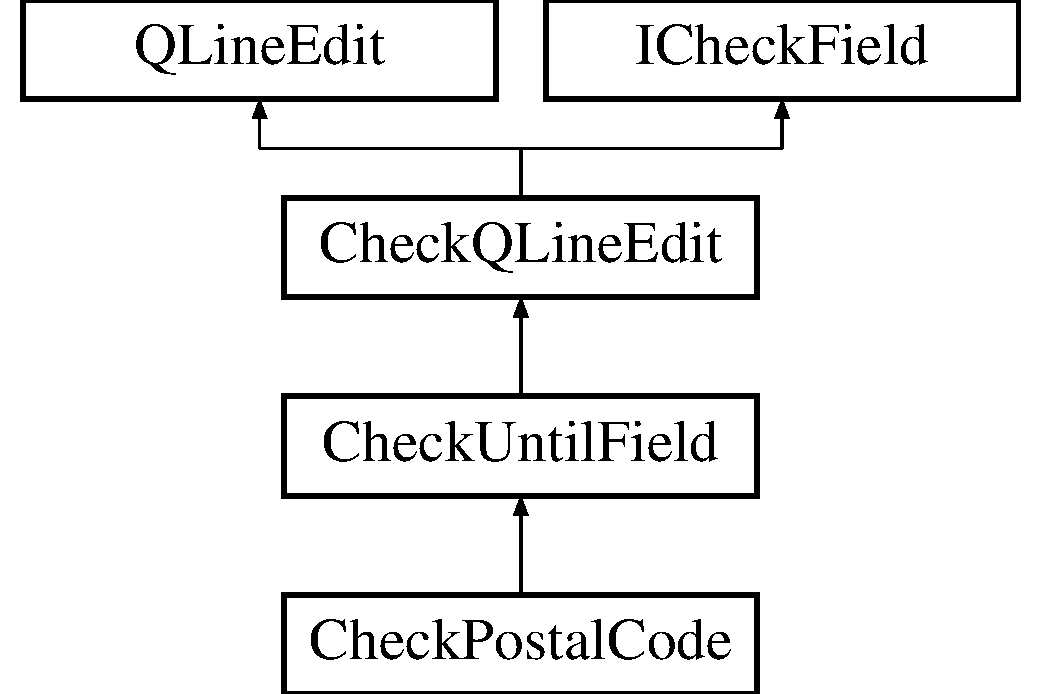
\includegraphics[height=4.000000cm]{dc/d63/classCheckPostalCode}
\end{center}
\end{figure}
\subsection*{Public Member Functions}
\begin{DoxyCompactItemize}
\item 
\hyperlink{classCheckPostalCode_a98cce06b95b46bf285cf6bc6e52cbfcb}{Check\+Postal\+Code} (Q\+Widget $\ast$w=0, Q\+Push\+Button $\ast$btn=0)
\begin{DoxyCompactList}\small\item\em \hyperlink{classCheckPostalCode_a98cce06b95b46bf285cf6bc6e52cbfcb}{Check\+Postal\+Code\+::\+Check\+Postal\+Code} Construct a \hyperlink{classCheckPostalCode}{Check\+Postal\+Code}. \end{DoxyCompactList}\item 
bool \hyperlink{classCheckPostalCode_ad91ba5622617675fbb5c767036163142}{check} (Q\+String text)
\begin{DoxyCompactList}\small\item\em \hyperlink{classCheckPostalCode_ad91ba5622617675fbb5c767036163142}{Check\+Postal\+Code\+::check} Check if the field is valid. To be valid, a name should be composed of a character. \end{DoxyCompactList}\item 
Q\+String \hyperlink{classCheckPostalCode_a3691eb5a484579a77622529ae25261a4}{get\+Country} () const 
\begin{DoxyCompactList}\small\item\em \hyperlink{classCheckPostalCode_a3691eb5a484579a77622529ae25261a4}{Check\+Postal\+Code\+::get\+Country} Return the country linked to current field. \end{DoxyCompactList}\item 
void \hyperlink{classCheckPostalCode_ac82e538c932bd9165d3d40ea949baa4b}{set\+Country} (const Q\+String \&country)
\begin{DoxyCompactList}\small\item\em \hyperlink{classCheckPostalCode_ac82e538c932bd9165d3d40ea949baa4b}{Check\+Postal\+Code\+::set\+Country} Modify the {\itshape country} linked to field. \end{DoxyCompactList}\end{DoxyCompactItemize}
\subsection*{Additional Inherited Members}


\subsection{Detailed Description}
The \hyperlink{classCheckPostalCode}{Check\+Postal\+Code} class Line Edit of postal code with a check icon. 

\subsection{Constructor \& Destructor Documentation}
\hypertarget{classCheckPostalCode_a98cce06b95b46bf285cf6bc6e52cbfcb}{\index{Check\+Postal\+Code@{Check\+Postal\+Code}!Check\+Postal\+Code@{Check\+Postal\+Code}}
\index{Check\+Postal\+Code@{Check\+Postal\+Code}!Check\+Postal\+Code@{Check\+Postal\+Code}}
\subsubsection[{Check\+Postal\+Code}]{\setlength{\rightskip}{0pt plus 5cm}Check\+Postal\+Code\+::\+Check\+Postal\+Code (
\begin{DoxyParamCaption}
\item[{Q\+Widget $\ast$}]{w = {\ttfamily 0}, }
\item[{Q\+Push\+Button $\ast$}]{btn = {\ttfamily 0}}
\end{DoxyParamCaption}
)}}\label{classCheckPostalCode_a98cce06b95b46bf285cf6bc6e52cbfcb}


\hyperlink{classCheckPostalCode_a98cce06b95b46bf285cf6bc6e52cbfcb}{Check\+Postal\+Code\+::\+Check\+Postal\+Code} Construct a \hyperlink{classCheckPostalCode}{Check\+Postal\+Code}. 


\begin{DoxyParams}{Parameters}
{\em w} & Q\+Widget linked to {\bfseries \hyperlink{classCheckPostalCode}{Check\+Postal\+Code}} \\
\hline
\end{DoxyParams}


\subsection{Member Function Documentation}
\hypertarget{classCheckPostalCode_ad91ba5622617675fbb5c767036163142}{\index{Check\+Postal\+Code@{Check\+Postal\+Code}!check@{check}}
\index{check@{check}!Check\+Postal\+Code@{Check\+Postal\+Code}}
\subsubsection[{check}]{\setlength{\rightskip}{0pt plus 5cm}bool Check\+Postal\+Code\+::check (
\begin{DoxyParamCaption}
\item[{Q\+String}]{text}
\end{DoxyParamCaption}
)\hspace{0.3cm}{\ttfamily [virtual]}}}\label{classCheckPostalCode_ad91ba5622617675fbb5c767036163142}


\hyperlink{classCheckPostalCode_ad91ba5622617675fbb5c767036163142}{Check\+Postal\+Code\+::check} Check if the field is valid. To be valid, a name should be composed of a character. 


\begin{DoxyParams}{Parameters}
{\em text} & \\
\hline
\end{DoxyParams}
\begin{DoxyReturn}{Returns}
boolean 
\end{DoxyReturn}


Implements \hyperlink{classICheckField_a6bd42b4d49c165cdd92822135123fd4b}{I\+Check\+Field}.

\hypertarget{classCheckPostalCode_a3691eb5a484579a77622529ae25261a4}{\index{Check\+Postal\+Code@{Check\+Postal\+Code}!get\+Country@{get\+Country}}
\index{get\+Country@{get\+Country}!Check\+Postal\+Code@{Check\+Postal\+Code}}
\subsubsection[{get\+Country}]{\setlength{\rightskip}{0pt plus 5cm}Q\+String Check\+Postal\+Code\+::get\+Country (
\begin{DoxyParamCaption}
{}
\end{DoxyParamCaption}
) const}}\label{classCheckPostalCode_a3691eb5a484579a77622529ae25261a4}


\hyperlink{classCheckPostalCode_a3691eb5a484579a77622529ae25261a4}{Check\+Postal\+Code\+::get\+Country} Return the country linked to current field. 

\begin{DoxyReturn}{Returns}
country 
\end{DoxyReturn}
\hypertarget{classCheckPostalCode_ac82e538c932bd9165d3d40ea949baa4b}{\index{Check\+Postal\+Code@{Check\+Postal\+Code}!set\+Country@{set\+Country}}
\index{set\+Country@{set\+Country}!Check\+Postal\+Code@{Check\+Postal\+Code}}
\subsubsection[{set\+Country}]{\setlength{\rightskip}{0pt plus 5cm}void Check\+Postal\+Code\+::set\+Country (
\begin{DoxyParamCaption}
\item[{const Q\+String \&}]{country}
\end{DoxyParamCaption}
)}}\label{classCheckPostalCode_ac82e538c932bd9165d3d40ea949baa4b}


\hyperlink{classCheckPostalCode_ac82e538c932bd9165d3d40ea949baa4b}{Check\+Postal\+Code\+::set\+Country} Modify the {\itshape country} linked to field. 


\begin{DoxyParams}{Parameters}
{\em country} & New country \\
\hline
\end{DoxyParams}


The documentation for this class was generated from the following files\+:\begin{DoxyCompactItemize}
\item 
src/widgets/checkfields/checkpostalcode.\+h\item 
src/widgets/checkfields/checkpostalcode.\+cpp\end{DoxyCompactItemize}

\hypertarget{classCheckQLineEdit}{\section{Check\+Q\+Line\+Edit Class Reference}
\label{classCheckQLineEdit}\index{Check\+Q\+Line\+Edit@{Check\+Q\+Line\+Edit}}
}


The \hyperlink{classCheckQLineEdit}{Check\+Q\+Line\+Edit} class Line\+Edit custom with a check of text inputed.  




{\ttfamily \#include $<$checkqlineedit.\+h$>$}

Inheritance diagram for Check\+Q\+Line\+Edit\+:\begin{figure}[H]
\begin{center}
\leavevmode
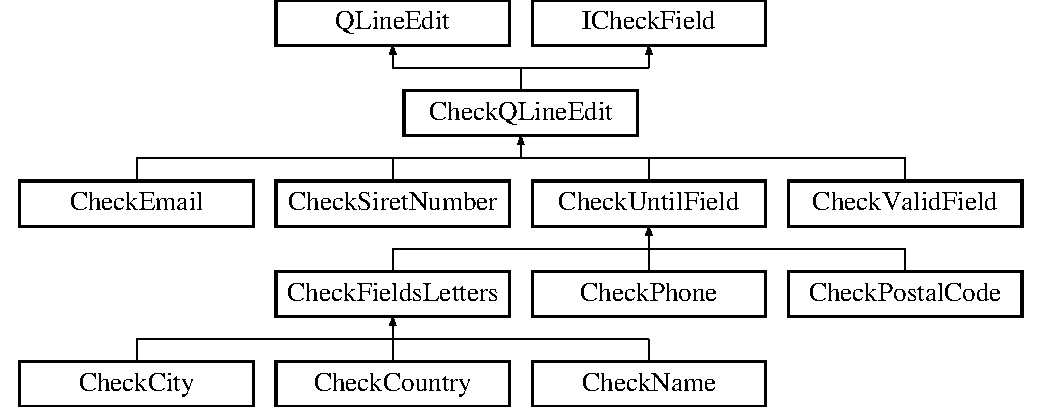
\includegraphics[height=5.000000cm]{d1/da9/classCheckQLineEdit}
\end{center}
\end{figure}
\subsection*{Public Slots}
\begin{DoxyCompactItemize}
\item 
\hypertarget{classCheckQLineEdit_a137569359307e1b17449af3a72c5e80e}{void \hyperlink{classCheckQLineEdit_a137569359307e1b17449af3a72c5e80e}{field\+Text\+Changed} (const Q\+String \&text)}\label{classCheckQLineEdit_a137569359307e1b17449af3a72c5e80e}

\begin{DoxyCompactList}\small\item\em \hyperlink{classCheckQLineEdit_a137569359307e1b17449af3a72c5e80e}{Check\+Q\+Line\+Edit\+::field\+Text\+Changed} For each new characater inputed or removed, displays an icon to show if the field is valid or not. \end{DoxyCompactList}\end{DoxyCompactItemize}
\subsection*{Public Member Functions}
\begin{DoxyCompactItemize}
\item 
\hyperlink{classCheckQLineEdit_acc48f17bfddb47e4101a7aedbace7783}{Check\+Q\+Line\+Edit} (Q\+Widget $\ast$parent=0, Q\+Push\+Button $\ast$btn=0)
\begin{DoxyCompactList}\small\item\em \hyperlink{classCheckQLineEdit_acc48f17bfddb47e4101a7aedbace7783}{Check\+Q\+Line\+Edit\+::\+Check\+Q\+Line\+Edit} Construct a \hyperlink{classCheckQLineEdit}{Check\+Q\+Line\+Edit}. \end{DoxyCompactList}\item 
\hypertarget{classCheckQLineEdit_a730ae162e31a8c76f5532d3f3c8903c6}{void \hyperlink{classCheckQLineEdit_a730ae162e31a8c76f5532d3f3c8903c6}{display\+Check\+Valid\+Field\+Icon} ()}\label{classCheckQLineEdit_a730ae162e31a8c76f5532d3f3c8903c6}

\begin{DoxyCompactList}\small\item\em \hyperlink{classCheckQLineEdit_a730ae162e31a8c76f5532d3f3c8903c6}{Check\+Q\+Line\+Edit\+::display\+Check\+Valid\+Field\+Icon} Display a valid icon into the field. \end{DoxyCompactList}\item 
\hypertarget{classCheckQLineEdit_aaf3b88a48a806bc6215f685bc45937a5}{void \hyperlink{classCheckQLineEdit_aaf3b88a48a806bc6215f685bc45937a5}{display\+Check\+No\+Valid\+Field\+Icon} ()}\label{classCheckQLineEdit_aaf3b88a48a806bc6215f685bc45937a5}

\begin{DoxyCompactList}\small\item\em \hyperlink{classCheckQLineEdit_aaf3b88a48a806bc6215f685bc45937a5}{Check\+Q\+Line\+Edit\+::display\+Check\+No\+Valid\+Field\+Icon} Display a \char`\"{}no valid\char`\"{} icon into the field. \end{DoxyCompactList}\item 
Q\+Push\+Button $\ast$ \hyperlink{classCheckQLineEdit_a87ea56ee9e7833b77c408be489b116e3}{get\+Btn\+Valid} () const 
\begin{DoxyCompactList}\small\item\em \hyperlink{classCheckQLineEdit_a87ea56ee9e7833b77c408be489b116e3}{Check\+Q\+Line\+Edit\+::get\+Btn\+Valid}. \end{DoxyCompactList}\item 
void \hyperlink{classCheckQLineEdit_a28bb08ffaac7da25289a7d93639ba00f}{set\+Btn\+Valid} (Q\+Push\+Button $\ast$\hyperlink{classCheckQLineEdit_a87ea56ee9e7833b77c408be489b116e3}{get\+Btn\+Valid})
\begin{DoxyCompactList}\small\item\em \hyperlink{classCheckQLineEdit_a28bb08ffaac7da25289a7d93639ba00f}{Check\+Q\+Line\+Edit\+::set\+Btn\+Valid}. \end{DoxyCompactList}\item 
bool \hyperlink{classCheckQLineEdit_a50e64b1790af6edb2c587e098c8b99f8}{is\+Valid} ()
\begin{DoxyCompactList}\small\item\em is\+Valid Return true if the current field if valid \end{DoxyCompactList}\end{DoxyCompactItemize}


\subsection{Detailed Description}
The \hyperlink{classCheckQLineEdit}{Check\+Q\+Line\+Edit} class Line\+Edit custom with a check of text inputed. 

\subsection{Constructor \& Destructor Documentation}
\hypertarget{classCheckQLineEdit_acc48f17bfddb47e4101a7aedbace7783}{\index{Check\+Q\+Line\+Edit@{Check\+Q\+Line\+Edit}!Check\+Q\+Line\+Edit@{Check\+Q\+Line\+Edit}}
\index{Check\+Q\+Line\+Edit@{Check\+Q\+Line\+Edit}!Check\+Q\+Line\+Edit@{Check\+Q\+Line\+Edit}}
\subsubsection[{Check\+Q\+Line\+Edit}]{\setlength{\rightskip}{0pt plus 5cm}Check\+Q\+Line\+Edit\+::\+Check\+Q\+Line\+Edit (
\begin{DoxyParamCaption}
\item[{Q\+Widget $\ast$}]{parent = {\ttfamily 0}, }
\item[{Q\+Push\+Button $\ast$}]{btn = {\ttfamily 0}}
\end{DoxyParamCaption}
)\hspace{0.3cm}{\ttfamily [explicit]}}}\label{classCheckQLineEdit_acc48f17bfddb47e4101a7aedbace7783}


\hyperlink{classCheckQLineEdit_acc48f17bfddb47e4101a7aedbace7783}{Check\+Q\+Line\+Edit\+::\+Check\+Q\+Line\+Edit} Construct a \hyperlink{classCheckQLineEdit}{Check\+Q\+Line\+Edit}. 


\begin{DoxyParams}{Parameters}
{\em parent} & \\
\hline
\end{DoxyParams}


\subsection{Member Function Documentation}
\hypertarget{classCheckQLineEdit_a87ea56ee9e7833b77c408be489b116e3}{\index{Check\+Q\+Line\+Edit@{Check\+Q\+Line\+Edit}!get\+Btn\+Valid@{get\+Btn\+Valid}}
\index{get\+Btn\+Valid@{get\+Btn\+Valid}!Check\+Q\+Line\+Edit@{Check\+Q\+Line\+Edit}}
\subsubsection[{get\+Btn\+Valid}]{\setlength{\rightskip}{0pt plus 5cm}Q\+Push\+Button $\ast$ Check\+Q\+Line\+Edit\+::get\+Btn\+Valid (
\begin{DoxyParamCaption}
{}
\end{DoxyParamCaption}
) const}}\label{classCheckQLineEdit_a87ea56ee9e7833b77c408be489b116e3}


\hyperlink{classCheckQLineEdit_a87ea56ee9e7833b77c408be489b116e3}{Check\+Q\+Line\+Edit\+::get\+Btn\+Valid}. 

\begin{DoxyReturn}{Returns}
a 
\end{DoxyReturn}
\hypertarget{classCheckQLineEdit_a50e64b1790af6edb2c587e098c8b99f8}{\index{Check\+Q\+Line\+Edit@{Check\+Q\+Line\+Edit}!is\+Valid@{is\+Valid}}
\index{is\+Valid@{is\+Valid}!Check\+Q\+Line\+Edit@{Check\+Q\+Line\+Edit}}
\subsubsection[{is\+Valid}]{\setlength{\rightskip}{0pt plus 5cm}bool Check\+Q\+Line\+Edit\+::is\+Valid (
\begin{DoxyParamCaption}
{}
\end{DoxyParamCaption}
)}}\label{classCheckQLineEdit_a50e64b1790af6edb2c587e098c8b99f8}


is\+Valid Return true if the current field if valid 

\begin{DoxyReturn}{Returns}
boolean 
\end{DoxyReturn}
\hypertarget{classCheckQLineEdit_a28bb08ffaac7da25289a7d93639ba00f}{\index{Check\+Q\+Line\+Edit@{Check\+Q\+Line\+Edit}!set\+Btn\+Valid@{set\+Btn\+Valid}}
\index{set\+Btn\+Valid@{set\+Btn\+Valid}!Check\+Q\+Line\+Edit@{Check\+Q\+Line\+Edit}}
\subsubsection[{set\+Btn\+Valid}]{\setlength{\rightskip}{0pt plus 5cm}void Check\+Q\+Line\+Edit\+::set\+Btn\+Valid (
\begin{DoxyParamCaption}
\item[{Q\+Push\+Button $\ast$}]{get\+Btn\+Valid}
\end{DoxyParamCaption}
)}}\label{classCheckQLineEdit_a28bb08ffaac7da25289a7d93639ba00f}


\hyperlink{classCheckQLineEdit_a28bb08ffaac7da25289a7d93639ba00f}{Check\+Q\+Line\+Edit\+::set\+Btn\+Valid}. 


\begin{DoxyParams}{Parameters}
{\em get\+Btn\+Valid} & \\
\hline
\end{DoxyParams}


The documentation for this class was generated from the following files\+:\begin{DoxyCompactItemize}
\item 
src/gui/widgets/checkfields/checkqlineedit.\+h\item 
src/gui/widgets/checkfields/checkqlineedit.\+cpp\end{DoxyCompactItemize}

\hypertarget{classCheckSiretNumber}{\section{Check\+Siret\+Number Class Reference}
\label{classCheckSiretNumber}\index{Check\+Siret\+Number@{Check\+Siret\+Number}}
}


The \hyperlink{classCheckSiretNumber}{Check\+Siret\+Number} class Line Edit with a check icon.  




{\ttfamily \#include $<$checksiretnumber.\+h$>$}

Inheritance diagram for Check\+Siret\+Number\+:\begin{figure}[H]
\begin{center}
\leavevmode
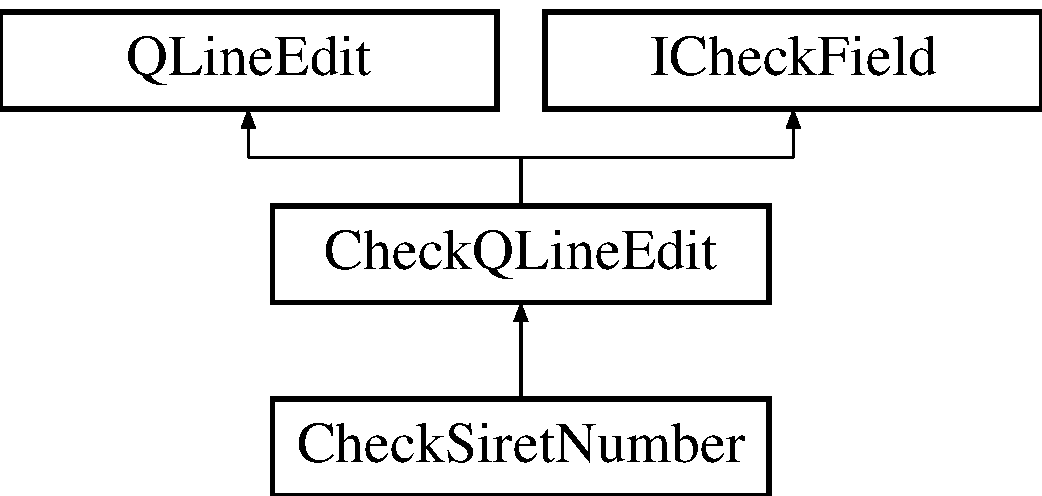
\includegraphics[height=3.000000cm]{d7/d29/classCheckSiretNumber}
\end{center}
\end{figure}
\subsection*{Public Member Functions}
\begin{DoxyCompactItemize}
\item 
\hyperlink{classCheckSiretNumber_a0581c0a2d6c0c1a62dab77515422b194}{Check\+Siret\+Number} (Q\+Widget $\ast$w=0, Q\+Push\+Button $\ast$btn=0)
\begin{DoxyCompactList}\small\item\em \hyperlink{classCheckSiretNumber_a0581c0a2d6c0c1a62dab77515422b194}{Check\+Siret\+Number\+::\+Check\+Siret\+Number} Construct a \hyperlink{classCheckSiretNumber}{Check\+Siret\+Number}. \end{DoxyCompactList}\item 
bool \hyperlink{classCheckSiretNumber_aaf0a1411e380789062564bd992e72c1b}{check} (Q\+String text)
\begin{DoxyCompactList}\small\item\em \hyperlink{classCheckSiretNumber_aaf0a1411e380789062564bd992e72c1b}{Check\+Siret\+Number\+::check} Check if the field no\+Siret is valid. To be valid, a S\+I\+R\+E\+T number should be composed of numbers. \end{DoxyCompactList}\end{DoxyCompactItemize}
\subsection*{Additional Inherited Members}


\subsection{Detailed Description}
The \hyperlink{classCheckSiretNumber}{Check\+Siret\+Number} class Line Edit with a check icon. 

\subsection{Constructor \& Destructor Documentation}
\hypertarget{classCheckSiretNumber_a0581c0a2d6c0c1a62dab77515422b194}{\index{Check\+Siret\+Number@{Check\+Siret\+Number}!Check\+Siret\+Number@{Check\+Siret\+Number}}
\index{Check\+Siret\+Number@{Check\+Siret\+Number}!Check\+Siret\+Number@{Check\+Siret\+Number}}
\subsubsection[{Check\+Siret\+Number}]{\setlength{\rightskip}{0pt plus 5cm}Check\+Siret\+Number\+::\+Check\+Siret\+Number (
\begin{DoxyParamCaption}
\item[{Q\+Widget $\ast$}]{w = {\ttfamily 0}, }
\item[{Q\+Push\+Button $\ast$}]{btn = {\ttfamily 0}}
\end{DoxyParamCaption}
)}}\label{classCheckSiretNumber_a0581c0a2d6c0c1a62dab77515422b194}


\hyperlink{classCheckSiretNumber_a0581c0a2d6c0c1a62dab77515422b194}{Check\+Siret\+Number\+::\+Check\+Siret\+Number} Construct a \hyperlink{classCheckSiretNumber}{Check\+Siret\+Number}. 


\begin{DoxyParams}{Parameters}
{\em w} & Q\+Widget linked to {\bfseries \hyperlink{classCheckSiretNumber}{Check\+Siret\+Number}} \\
\hline
\end{DoxyParams}


\subsection{Member Function Documentation}
\hypertarget{classCheckSiretNumber_aaf0a1411e380789062564bd992e72c1b}{\index{Check\+Siret\+Number@{Check\+Siret\+Number}!check@{check}}
\index{check@{check}!Check\+Siret\+Number@{Check\+Siret\+Number}}
\subsubsection[{check}]{\setlength{\rightskip}{0pt plus 5cm}bool Check\+Siret\+Number\+::check (
\begin{DoxyParamCaption}
\item[{Q\+String}]{text}
\end{DoxyParamCaption}
)\hspace{0.3cm}{\ttfamily [virtual]}}}\label{classCheckSiretNumber_aaf0a1411e380789062564bd992e72c1b}


\hyperlink{classCheckSiretNumber_aaf0a1411e380789062564bd992e72c1b}{Check\+Siret\+Number\+::check} Check if the field no\+Siret is valid. To be valid, a S\+I\+R\+E\+T number should be composed of numbers. 


\begin{DoxyParams}{Parameters}
{\em text} & \\
\hline
\end{DoxyParams}
\begin{DoxyReturn}{Returns}
boolean 
\end{DoxyReturn}


Implements \hyperlink{classICheckField_a6bd42b4d49c165cdd92822135123fd4b}{I\+Check\+Field}.



The documentation for this class was generated from the following files\+:\begin{DoxyCompactItemize}
\item 
src/widgets/checkfields/checksiretnumber.\+h\item 
src/widgets/checkfields/checksiretnumber.\+cpp\end{DoxyCompactItemize}

\hypertarget{classCheckUntilField}{\section{Check\+Until\+Field Class Reference}
\label{classCheckUntilField}\index{Check\+Until\+Field@{Check\+Until\+Field}}
}


The \hyperlink{classCheckUntilField}{Check\+Until\+Field} class.  




{\ttfamily \#include $<$checkuntilfield.\+h$>$}

Inheritance diagram for Check\+Until\+Field\+:\begin{figure}[H]
\begin{center}
\leavevmode
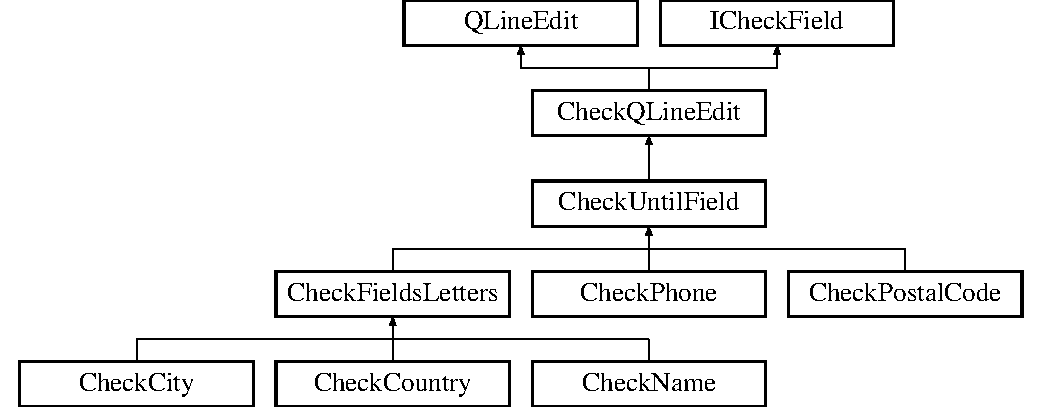
\includegraphics[height=5.000000cm]{dc/db9/classCheckUntilField}
\end{center}
\end{figure}
\subsection*{Public Member Functions}
\begin{DoxyCompactItemize}
\item 
\hyperlink{classCheckUntilField_a7b3789fe02959e488b35a0e79362f786}{Check\+Until\+Field} (Q\+Widget $\ast$w=0, Q\+Push\+Button $\ast$btn=0)
\begin{DoxyCompactList}\small\item\em \hyperlink{classCheckUntilField_a7b3789fe02959e488b35a0e79362f786}{Check\+Until\+Field\+::\+Check\+Until\+Field} Construct a \hyperlink{classCheckUntilField}{Check\+Until\+Field}. \end{DoxyCompactList}\item 
bool \hyperlink{classCheckUntilField_acfb9e2f95bebcb5b5d2337e3ac4f4d47}{check} (Q\+String text)
\begin{DoxyCompactList}\small\item\em \hyperlink{classCheckUntilField_acfb9e2f95bebcb5b5d2337e3ac4f4d47}{Check\+Until\+Field\+::check} Check if the field is valid. To be valid, a name should be composed of a character. \end{DoxyCompactList}\end{DoxyCompactItemize}
\subsection*{Additional Inherited Members}


\subsection{Detailed Description}
The \hyperlink{classCheckUntilField}{Check\+Until\+Field} class. 

\subsection{Constructor \& Destructor Documentation}
\hypertarget{classCheckUntilField_a7b3789fe02959e488b35a0e79362f786}{\index{Check\+Until\+Field@{Check\+Until\+Field}!Check\+Until\+Field@{Check\+Until\+Field}}
\index{Check\+Until\+Field@{Check\+Until\+Field}!Check\+Until\+Field@{Check\+Until\+Field}}
\subsubsection[{Check\+Until\+Field}]{\setlength{\rightskip}{0pt plus 5cm}Check\+Until\+Field\+::\+Check\+Until\+Field (
\begin{DoxyParamCaption}
\item[{Q\+Widget $\ast$}]{w = {\ttfamily 0}, }
\item[{Q\+Push\+Button $\ast$}]{btn = {\ttfamily 0}}
\end{DoxyParamCaption}
)}}\label{classCheckUntilField_a7b3789fe02959e488b35a0e79362f786}


\hyperlink{classCheckUntilField_a7b3789fe02959e488b35a0e79362f786}{Check\+Until\+Field\+::\+Check\+Until\+Field} Construct a \hyperlink{classCheckUntilField}{Check\+Until\+Field}. 


\begin{DoxyParams}{Parameters}
{\em w} & Q\+Widget linked to {\bfseries \hyperlink{classCheckUntilField}{Check\+Until\+Field}} \\
\hline
\end{DoxyParams}


\subsection{Member Function Documentation}
\hypertarget{classCheckUntilField_acfb9e2f95bebcb5b5d2337e3ac4f4d47}{\index{Check\+Until\+Field@{Check\+Until\+Field}!check@{check}}
\index{check@{check}!Check\+Until\+Field@{Check\+Until\+Field}}
\subsubsection[{check}]{\setlength{\rightskip}{0pt plus 5cm}bool Check\+Until\+Field\+::check (
\begin{DoxyParamCaption}
\item[{Q\+String}]{text}
\end{DoxyParamCaption}
)\hspace{0.3cm}{\ttfamily [virtual]}}}\label{classCheckUntilField_acfb9e2f95bebcb5b5d2337e3ac4f4d47}


\hyperlink{classCheckUntilField_acfb9e2f95bebcb5b5d2337e3ac4f4d47}{Check\+Until\+Field\+::check} Check if the field is valid. To be valid, a name should be composed of a character. 


\begin{DoxyParams}{Parameters}
{\em text} & \\
\hline
\end{DoxyParams}
\begin{DoxyReturn}{Returns}
boolean 
\end{DoxyReturn}


Implements \hyperlink{classICheckField_a6bd42b4d49c165cdd92822135123fd4b}{I\+Check\+Field}.



The documentation for this class was generated from the following files\+:\begin{DoxyCompactItemize}
\item 
src/gui/widgets/checkfields/checkuntilfield.\+h\item 
src/gui/widgets/checkfields/checkuntilfield.\+cpp\end{DoxyCompactItemize}

\hypertarget{classCheckValidField}{\section{Check\+Valid\+Field Class Reference}
\label{classCheckValidField}\index{Check\+Valid\+Field@{Check\+Valid\+Field}}
}


The \hyperlink{classCheckValidField}{Check\+Valid\+Field} class Check field not required.  




{\ttfamily \#include $<$checkvalidfield.\+h$>$}

Inheritance diagram for Check\+Valid\+Field\+:\begin{figure}[H]
\begin{center}
\leavevmode
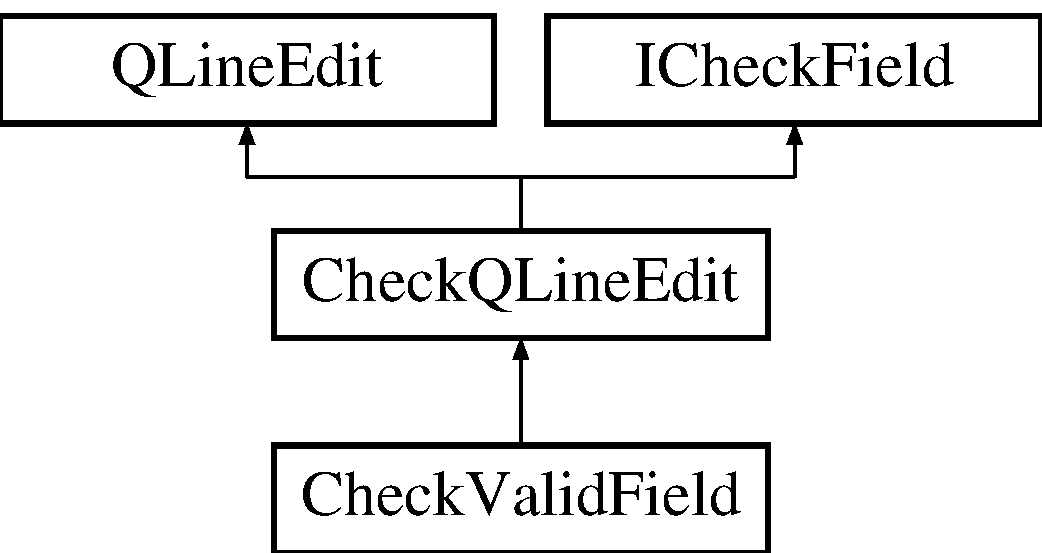
\includegraphics[height=3.000000cm]{dc/d93/classCheckValidField}
\end{center}
\end{figure}
\subsection*{Public Member Functions}
\begin{DoxyCompactItemize}
\item 
\hyperlink{classCheckValidField_acfb0bb44b22b5355a227273f439210b8}{Check\+Valid\+Field} (Q\+Widget $\ast$w=0, Q\+Push\+Button $\ast$btn=0)
\begin{DoxyCompactList}\small\item\em \hyperlink{classCheckValidField_acfb0bb44b22b5355a227273f439210b8}{Check\+Valid\+Field\+::\+Check\+Valid\+Field}. \end{DoxyCompactList}\item 
bool \hyperlink{classCheckValidField_a192b1c9c84ea8897661425fd3c0b9e8e}{check} (Q\+String text)
\begin{DoxyCompactList}\small\item\em \hyperlink{classCheckValidField_a192b1c9c84ea8897661425fd3c0b9e8e}{Check\+Valid\+Field\+::check} Return T\+R\+U\+E \+: the field is not required. \end{DoxyCompactList}\end{DoxyCompactItemize}
\subsection*{Additional Inherited Members}


\subsection{Detailed Description}
The \hyperlink{classCheckValidField}{Check\+Valid\+Field} class Check field not required. 

\subsection{Constructor \& Destructor Documentation}
\hypertarget{classCheckValidField_acfb0bb44b22b5355a227273f439210b8}{\index{Check\+Valid\+Field@{Check\+Valid\+Field}!Check\+Valid\+Field@{Check\+Valid\+Field}}
\index{Check\+Valid\+Field@{Check\+Valid\+Field}!Check\+Valid\+Field@{Check\+Valid\+Field}}
\subsubsection[{Check\+Valid\+Field}]{\setlength{\rightskip}{0pt plus 5cm}Check\+Valid\+Field\+::\+Check\+Valid\+Field (
\begin{DoxyParamCaption}
\item[{Q\+Widget $\ast$}]{w = {\ttfamily 0}, }
\item[{Q\+Push\+Button $\ast$}]{btn = {\ttfamily 0}}
\end{DoxyParamCaption}
)}}\label{classCheckValidField_acfb0bb44b22b5355a227273f439210b8}


\hyperlink{classCheckValidField_acfb0bb44b22b5355a227273f439210b8}{Check\+Valid\+Field\+::\+Check\+Valid\+Field}. 


\begin{DoxyParams}{Parameters}
{\em w} & Q\+Widget linked to {\bfseries \hyperlink{classCheckValidField}{Check\+Valid\+Field}} \\
\hline
\end{DoxyParams}


\subsection{Member Function Documentation}
\hypertarget{classCheckValidField_a192b1c9c84ea8897661425fd3c0b9e8e}{\index{Check\+Valid\+Field@{Check\+Valid\+Field}!check@{check}}
\index{check@{check}!Check\+Valid\+Field@{Check\+Valid\+Field}}
\subsubsection[{check}]{\setlength{\rightskip}{0pt plus 5cm}bool Check\+Valid\+Field\+::check (
\begin{DoxyParamCaption}
\item[{Q\+String}]{text}
\end{DoxyParamCaption}
)\hspace{0.3cm}{\ttfamily [virtual]}}}\label{classCheckValidField_a192b1c9c84ea8897661425fd3c0b9e8e}


\hyperlink{classCheckValidField_a192b1c9c84ea8897661425fd3c0b9e8e}{Check\+Valid\+Field\+::check} Return T\+R\+U\+E \+: the field is not required. 


\begin{DoxyParams}{Parameters}
{\em text} & \\
\hline
\end{DoxyParams}
\begin{DoxyReturn}{Returns}
boolean 
\end{DoxyReturn}


Implements \hyperlink{classICheckField_a6bd42b4d49c165cdd92822135123fd4b}{I\+Check\+Field}.



The documentation for this class was generated from the following files\+:\begin{DoxyCompactItemize}
\item 
src/widgets/checkfields/checkvalidfield.\+h\item 
src/widgets/checkfields/checkvalidfield.\+cpp\end{DoxyCompactItemize}

\hypertarget{classGui_1_1Widgets_1_1ComboBoxModelWidget}{\section{Gui\-:\-:Widgets\-:\-:Combo\-Box\-Model\-Widget Class Reference}
\label{classGui_1_1Widgets_1_1ComboBoxModelWidget}\index{Gui\-::\-Widgets\-::\-Combo\-Box\-Model\-Widget@{Gui\-::\-Widgets\-::\-Combo\-Box\-Model\-Widget}}
}


The \hyperlink{classGui_1_1Widgets_1_1ComboBoxModelWidget}{Combo\-Box\-Model\-Widget} class Model of Combo\-Box.  




{\ttfamily \#include $<$comboboxmodelwidget.\-h$>$}

Inheritance diagram for Gui\-:\-:Widgets\-:\-:Combo\-Box\-Model\-Widget\-:\begin{figure}[H]
\begin{center}
\leavevmode
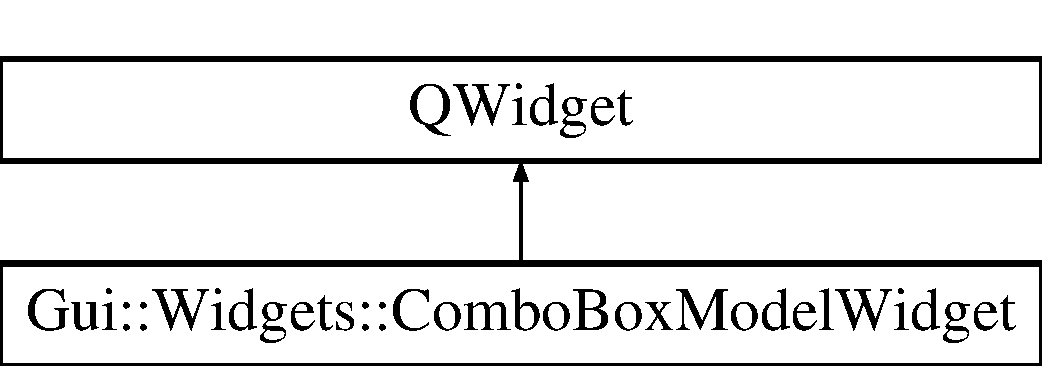
\includegraphics[height=2.000000cm]{d2/de0/classGui_1_1Widgets_1_1ComboBoxModelWidget}
\end{center}
\end{figure}
\subsection*{Public Member Functions}
\begin{DoxyCompactItemize}
\item 
\hyperlink{classGui_1_1Widgets_1_1ComboBoxModelWidget_afeca0199adce7d17dc440e8fa546c9e5}{Combo\-Box\-Model\-Widget} (Q\-Widget $\ast$parent=0)
\begin{DoxyCompactList}\small\item\em \hyperlink{classGui_1_1Widgets_1_1ComboBoxModelWidget_afeca0199adce7d17dc440e8fa546c9e5}{Combo\-Box\-Model\-Widget\-::\-Combo\-Box\-Model\-Widget} Construct a \hyperlink{classGui_1_1Widgets_1_1ComboBoxModelWidget}{Combo\-Box\-Model\-Widget}. \end{DoxyCompactList}\end{DoxyCompactItemize}


\subsection{Detailed Description}
The \hyperlink{classGui_1_1Widgets_1_1ComboBoxModelWidget}{Combo\-Box\-Model\-Widget} class Model of Combo\-Box. 

\subsection{Constructor \& Destructor Documentation}
\hypertarget{classGui_1_1Widgets_1_1ComboBoxModelWidget_afeca0199adce7d17dc440e8fa546c9e5}{\index{Gui\-::\-Widgets\-::\-Combo\-Box\-Model\-Widget@{Gui\-::\-Widgets\-::\-Combo\-Box\-Model\-Widget}!Combo\-Box\-Model\-Widget@{Combo\-Box\-Model\-Widget}}
\index{Combo\-Box\-Model\-Widget@{Combo\-Box\-Model\-Widget}!Gui::Widgets::ComboBoxModelWidget@{Gui\-::\-Widgets\-::\-Combo\-Box\-Model\-Widget}}
\subsubsection[{Combo\-Box\-Model\-Widget}]{\setlength{\rightskip}{0pt plus 5cm}Gui\-::\-Widgets\-::\-Combo\-Box\-Model\-Widget\-::\-Combo\-Box\-Model\-Widget (
\begin{DoxyParamCaption}
\item[{Q\-Widget $\ast$}]{parent = {\ttfamily 0}}
\end{DoxyParamCaption}
)\hspace{0.3cm}{\ttfamily [explicit]}}}\label{classGui_1_1Widgets_1_1ComboBoxModelWidget_afeca0199adce7d17dc440e8fa546c9e5}


\hyperlink{classGui_1_1Widgets_1_1ComboBoxModelWidget_afeca0199adce7d17dc440e8fa546c9e5}{Combo\-Box\-Model\-Widget\-::\-Combo\-Box\-Model\-Widget} Construct a \hyperlink{classGui_1_1Widgets_1_1ComboBoxModelWidget}{Combo\-Box\-Model\-Widget}. 


\begin{DoxyParams}{Parameters}
{\em parent} & Q\-Widget parent \\
\hline
\end{DoxyParams}


The documentation for this class was generated from the following files\-:\begin{DoxyCompactItemize}
\item 
/home/travis/build/\-F\-A\-C\-T-\/\-Team/\-Fact\-Dev/src/gui/widgets/comboboxmodelwidget.\-h\item 
/home/travis/build/\-F\-A\-C\-T-\/\-Team/\-Fact\-Dev/src/gui/widgets/comboboxmodelwidget.\-cpp\end{DoxyCompactItemize}

\hypertarget{classContributoriesDatabaseTest}{\section{Contributories\-Database\-Test Class Reference}
\label{classContributoriesDatabaseTest}\index{Contributories\-Database\-Test@{Contributories\-Database\-Test}}
}
Inheritance diagram for Contributories\-Database\-Test\-:\begin{figure}[H]
\begin{center}
\leavevmode
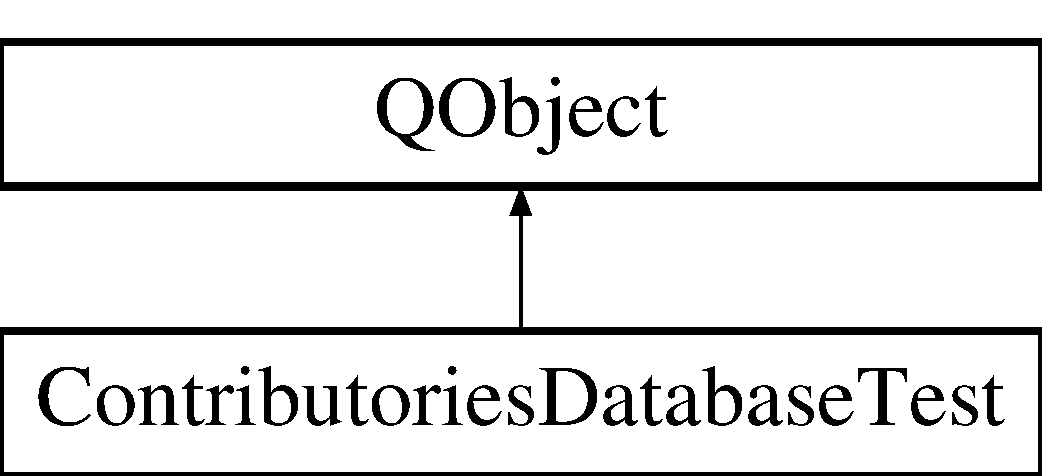
\includegraphics[height=2.000000cm]{d8/df7/classContributoriesDatabaseTest}
\end{center}
\end{figure}


The documentation for this class was generated from the following files\-:\begin{DoxyCompactItemize}
\item 
/home/florent/\-Documents/\-Projet\-\_\-\-S8/\-Fact\-Dev/tests/database/contributoriesdatabasetest.\-h\item 
/home/florent/\-Documents/\-Projet\-\_\-\-S8/\-Fact\-Dev/tests/database/contributoriesdatabasetest.\-cpp\end{DoxyCompactItemize}

\hypertarget{classGui_1_1Widgets_1_1WdgModels_1_1ContributoriesTableModel}{\section{Gui\-:\-:Widgets\-:\-:Wdg\-Models\-:\-:Contributories\-Table\-Model Class Reference}
\label{classGui_1_1Widgets_1_1WdgModels_1_1ContributoriesTableModel}\index{Gui\-::\-Widgets\-::\-Wdg\-Models\-::\-Contributories\-Table\-Model@{Gui\-::\-Widgets\-::\-Wdg\-Models\-::\-Contributories\-Table\-Model}}
}


The \hyperlink{classGui_1_1Widgets_1_1WdgModels_1_1ContributoriesTableModel}{Contributories\-Table\-Model} class for a custom table for contributories widget.  




{\ttfamily \#include $<$contributoriestablemodel.\-h$>$}

Inheritance diagram for Gui\-:\-:Widgets\-:\-:Wdg\-Models\-:\-:Contributories\-Table\-Model\-:\begin{figure}[H]
\begin{center}
\leavevmode
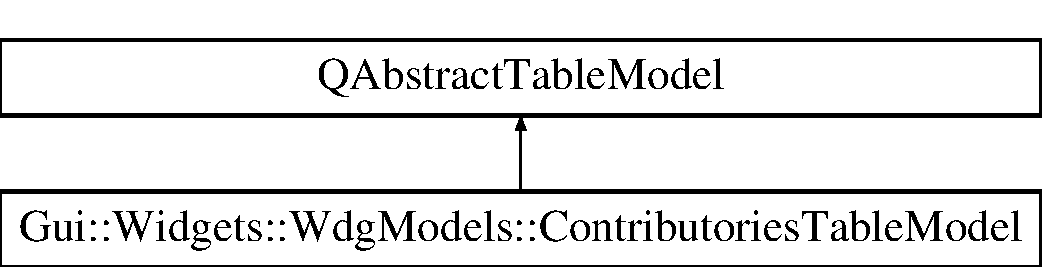
\includegraphics[height=2.000000cm]{dc/db9/classGui_1_1Widgets_1_1WdgModels_1_1ContributoriesTableModel}
\end{center}
\end{figure}
\subsection*{Public Member Functions}
\begin{DoxyCompactItemize}
\item 
\hyperlink{classGui_1_1Widgets_1_1WdgModels_1_1ContributoriesTableModel_abfc7cdc96006729fa8b03571bb8b586b}{Contributories\-Table\-Model} (Q\-Object $\ast$parent=0)
\begin{DoxyCompactList}\small\item\em \hyperlink{classGui_1_1Widgets_1_1WdgModels_1_1ContributoriesTableModel}{Contributories\-Table\-Model} Construct a \hyperlink{classGui_1_1Widgets_1_1WdgModels_1_1ContributoriesTableModel}{Contributories\-Table\-Model}. \end{DoxyCompactList}\item 
int \hyperlink{classGui_1_1Widgets_1_1WdgModels_1_1ContributoriesTableModel_a4adfd94506448337ceac8504b76531aa}{row\-Count} (const Q\-Model\-Index \&) const 
\begin{DoxyCompactList}\small\item\em row\-Count Number of contributories row \end{DoxyCompactList}\item 
int \hyperlink{classGui_1_1Widgets_1_1WdgModels_1_1ContributoriesTableModel_ab052217cb08f856ecfe465458f95c174}{column\-Count} (const Q\-Model\-Index \&) const 
\begin{DoxyCompactList}\small\item\em column\-Count Number of column of a contributory \end{DoxyCompactList}\item 
Q\-Variant \hyperlink{classGui_1_1Widgets_1_1WdgModels_1_1ContributoriesTableModel_aa95bb13ea63275f96187150a8a2d3972}{data} (const Q\-Model\-Index \&index, int role) const 
\begin{DoxyCompactList}\small\item\em data Obtains data of a specify cell \end{DoxyCompactList}\item 
Q\-Variant \hyperlink{classGui_1_1Widgets_1_1WdgModels_1_1ContributoriesTableModel_ac08635d8660ddd4444d7f2b75ae3d0ef}{header\-Data} (int section, Qt\-::\-Orientation orientation, int role) const 
\begin{DoxyCompactList}\small\item\em header\-Data Obtains header title of table \end{DoxyCompactList}\item 
bool \hyperlink{classGui_1_1Widgets_1_1WdgModels_1_1ContributoriesTableModel_a1c9f7969dc52e5840acfc122fcb2ab48}{set\-Data} (const Q\-Model\-Index \&index, const Q\-Variant \&value, int role=Qt\-::\-Edit\-Role)
\begin{DoxyCompactList}\small\item\em set\-Data Change data of a cell \end{DoxyCompactList}\item 
void \hyperlink{classGui_1_1Widgets_1_1WdgModels_1_1ContributoriesTableModel_a6d3f0ab976abd9993b731b27fbe3a404}{append} (const \hyperlink{classModels_1_1Contributory}{Contributory} \&contributory)
\begin{DoxyCompactList}\small\item\em append Add a new line in table \end{DoxyCompactList}\item 
void \hyperlink{classGui_1_1Widgets_1_1WdgModels_1_1ContributoriesTableModel_a76666bbbc940867b6ff3366424f72e26}{remove} (const int i)
\begin{DoxyCompactList}\small\item\em remove Remove a line \end{DoxyCompactList}\item 
Qt\-::\-Item\-Flags \hyperlink{classGui_1_1Widgets_1_1WdgModels_1_1ContributoriesTableModel_a6bf3e8c45bb499e82546be456a7de77b}{flags} (const Q\-Model\-Index \&index) const 
\begin{DoxyCompactList}\small\item\em flags Differents table flags \end{DoxyCompactList}\item 
Q\-List$<$ \hyperlink{classModels_1_1Contributory}{Contributory} $>$ \hyperlink{classGui_1_1Widgets_1_1WdgModels_1_1ContributoriesTableModel_af20bc21f24f7597b6b7d053d11d02d97}{get\-Contributories} ()
\begin{DoxyCompactList}\small\item\em get\-Contributories Get all contributories of table \end{DoxyCompactList}\item 
int \hyperlink{classGui_1_1Widgets_1_1WdgModels_1_1ContributoriesTableModel_acc01a97c00bb57e6733f697fc45be0ed}{count} ()
\begin{DoxyCompactList}\small\item\em count Number of contributories in table \end{DoxyCompactList}\end{DoxyCompactItemize}


\subsection{Detailed Description}
The \hyperlink{classGui_1_1Widgets_1_1WdgModels_1_1ContributoriesTableModel}{Contributories\-Table\-Model} class for a custom table for contributories widget. 

\begin{DoxyAuthor}{Author}
Antoine de Roquemaurel 
\end{DoxyAuthor}
\begin{DoxySeeAlso}{See Also}
Contributory 
\end{DoxySeeAlso}


\subsection{Constructor \& Destructor Documentation}
\hypertarget{classGui_1_1Widgets_1_1WdgModels_1_1ContributoriesTableModel_abfc7cdc96006729fa8b03571bb8b586b}{\index{Gui\-::\-Widgets\-::\-Wdg\-Models\-::\-Contributories\-Table\-Model@{Gui\-::\-Widgets\-::\-Wdg\-Models\-::\-Contributories\-Table\-Model}!Contributories\-Table\-Model@{Contributories\-Table\-Model}}
\index{Contributories\-Table\-Model@{Contributories\-Table\-Model}!Gui::Widgets::WdgModels::ContributoriesTableModel@{Gui\-::\-Widgets\-::\-Wdg\-Models\-::\-Contributories\-Table\-Model}}
\subsubsection[{Contributories\-Table\-Model}]{\setlength{\rightskip}{0pt plus 5cm}Gui\-::\-Widgets\-::\-Wdg\-Models\-::\-Contributories\-Table\-Model\-::\-Contributories\-Table\-Model (
\begin{DoxyParamCaption}
\item[{Q\-Object $\ast$}]{parent = {\ttfamily 0}}
\end{DoxyParamCaption}
)}}\label{classGui_1_1Widgets_1_1WdgModels_1_1ContributoriesTableModel_abfc7cdc96006729fa8b03571bb8b586b}


\hyperlink{classGui_1_1Widgets_1_1WdgModels_1_1ContributoriesTableModel}{Contributories\-Table\-Model} Construct a \hyperlink{classGui_1_1Widgets_1_1WdgModels_1_1ContributoriesTableModel}{Contributories\-Table\-Model}. 


\begin{DoxyParams}{Parameters}
{\em parent} & Parent widget \\
\hline
\end{DoxyParams}


\subsection{Member Function Documentation}
\hypertarget{classGui_1_1Widgets_1_1WdgModels_1_1ContributoriesTableModel_a6d3f0ab976abd9993b731b27fbe3a404}{\index{Gui\-::\-Widgets\-::\-Wdg\-Models\-::\-Contributories\-Table\-Model@{Gui\-::\-Widgets\-::\-Wdg\-Models\-::\-Contributories\-Table\-Model}!append@{append}}
\index{append@{append}!Gui::Widgets::WdgModels::ContributoriesTableModel@{Gui\-::\-Widgets\-::\-Wdg\-Models\-::\-Contributories\-Table\-Model}}
\subsubsection[{append}]{\setlength{\rightskip}{0pt plus 5cm}void Gui\-::\-Widgets\-::\-Wdg\-Models\-::\-Contributories\-Table\-Model\-::append (
\begin{DoxyParamCaption}
\item[{const {\bf Contributory} \&}]{contributory}
\end{DoxyParamCaption}
)}}\label{classGui_1_1Widgets_1_1WdgModels_1_1ContributoriesTableModel_a6d3f0ab976abd9993b731b27fbe3a404}


append Add a new line in table 


\begin{DoxyParams}{Parameters}
{\em contributory} & The new contributory \\
\hline
\end{DoxyParams}
\hypertarget{classGui_1_1Widgets_1_1WdgModels_1_1ContributoriesTableModel_ab052217cb08f856ecfe465458f95c174}{\index{Gui\-::\-Widgets\-::\-Wdg\-Models\-::\-Contributories\-Table\-Model@{Gui\-::\-Widgets\-::\-Wdg\-Models\-::\-Contributories\-Table\-Model}!column\-Count@{column\-Count}}
\index{column\-Count@{column\-Count}!Gui::Widgets::WdgModels::ContributoriesTableModel@{Gui\-::\-Widgets\-::\-Wdg\-Models\-::\-Contributories\-Table\-Model}}
\subsubsection[{column\-Count}]{\setlength{\rightskip}{0pt plus 5cm}int Gui\-::\-Widgets\-::\-Wdg\-Models\-::\-Contributories\-Table\-Model\-::column\-Count (
\begin{DoxyParamCaption}
\item[{const Q\-Model\-Index \&}]{}
\end{DoxyParamCaption}
) const}}\label{classGui_1_1Widgets_1_1WdgModels_1_1ContributoriesTableModel_ab052217cb08f856ecfe465458f95c174}


column\-Count Number of column of a contributory 

\begin{DoxyReturn}{Returns}
The number of column 
\end{DoxyReturn}
\hypertarget{classGui_1_1Widgets_1_1WdgModels_1_1ContributoriesTableModel_acc01a97c00bb57e6733f697fc45be0ed}{\index{Gui\-::\-Widgets\-::\-Wdg\-Models\-::\-Contributories\-Table\-Model@{Gui\-::\-Widgets\-::\-Wdg\-Models\-::\-Contributories\-Table\-Model}!count@{count}}
\index{count@{count}!Gui::Widgets::WdgModels::ContributoriesTableModel@{Gui\-::\-Widgets\-::\-Wdg\-Models\-::\-Contributories\-Table\-Model}}
\subsubsection[{count}]{\setlength{\rightskip}{0pt plus 5cm}int Gui\-::\-Widgets\-::\-Wdg\-Models\-::\-Contributories\-Table\-Model\-::count (
\begin{DoxyParamCaption}
{}
\end{DoxyParamCaption}
)}}\label{classGui_1_1Widgets_1_1WdgModels_1_1ContributoriesTableModel_acc01a97c00bb57e6733f697fc45be0ed}


count Number of contributories in table 

\begin{DoxyReturn}{Returns}
The number of contributories 
\end{DoxyReturn}
\hypertarget{classGui_1_1Widgets_1_1WdgModels_1_1ContributoriesTableModel_aa95bb13ea63275f96187150a8a2d3972}{\index{Gui\-::\-Widgets\-::\-Wdg\-Models\-::\-Contributories\-Table\-Model@{Gui\-::\-Widgets\-::\-Wdg\-Models\-::\-Contributories\-Table\-Model}!data@{data}}
\index{data@{data}!Gui::Widgets::WdgModels::ContributoriesTableModel@{Gui\-::\-Widgets\-::\-Wdg\-Models\-::\-Contributories\-Table\-Model}}
\subsubsection[{data}]{\setlength{\rightskip}{0pt plus 5cm}Q\-Variant Gui\-::\-Widgets\-::\-Wdg\-Models\-::\-Contributories\-Table\-Model\-::data (
\begin{DoxyParamCaption}
\item[{const Q\-Model\-Index \&}]{index, }
\item[{int}]{role}
\end{DoxyParamCaption}
) const}}\label{classGui_1_1Widgets_1_1WdgModels_1_1ContributoriesTableModel_aa95bb13ea63275f96187150a8a2d3972}


data Obtains data of a specify cell 


\begin{DoxyParams}{Parameters}
{\em index} & The cell who we want data \\
\hline
{\em role} & The role of set \\
\hline
\end{DoxyParams}
\begin{DoxyReturn}{Returns}
The data of cell 
\end{DoxyReturn}
\hypertarget{classGui_1_1Widgets_1_1WdgModels_1_1ContributoriesTableModel_a6bf3e8c45bb499e82546be456a7de77b}{\index{Gui\-::\-Widgets\-::\-Wdg\-Models\-::\-Contributories\-Table\-Model@{Gui\-::\-Widgets\-::\-Wdg\-Models\-::\-Contributories\-Table\-Model}!flags@{flags}}
\index{flags@{flags}!Gui::Widgets::WdgModels::ContributoriesTableModel@{Gui\-::\-Widgets\-::\-Wdg\-Models\-::\-Contributories\-Table\-Model}}
\subsubsection[{flags}]{\setlength{\rightskip}{0pt plus 5cm}Qt\-::\-Item\-Flags Gui\-::\-Widgets\-::\-Wdg\-Models\-::\-Contributories\-Table\-Model\-::flags (
\begin{DoxyParamCaption}
\item[{const Q\-Model\-Index \&}]{index}
\end{DoxyParamCaption}
) const}}\label{classGui_1_1Widgets_1_1WdgModels_1_1ContributoriesTableModel_a6bf3e8c45bb499e82546be456a7de77b}


flags Differents table flags 


\begin{DoxyParams}{Parameters}
{\em index} & The cell who we want to know flags \\
\hline
\end{DoxyParams}
\begin{DoxyReturn}{Returns}
Flags 
\end{DoxyReturn}
\hypertarget{classGui_1_1Widgets_1_1WdgModels_1_1ContributoriesTableModel_af20bc21f24f7597b6b7d053d11d02d97}{\index{Gui\-::\-Widgets\-::\-Wdg\-Models\-::\-Contributories\-Table\-Model@{Gui\-::\-Widgets\-::\-Wdg\-Models\-::\-Contributories\-Table\-Model}!get\-Contributories@{get\-Contributories}}
\index{get\-Contributories@{get\-Contributories}!Gui::Widgets::WdgModels::ContributoriesTableModel@{Gui\-::\-Widgets\-::\-Wdg\-Models\-::\-Contributories\-Table\-Model}}
\subsubsection[{get\-Contributories}]{\setlength{\rightskip}{0pt plus 5cm}Q\-List$<$ {\bf Contributory} $>$ Gui\-::\-Widgets\-::\-Wdg\-Models\-::\-Contributories\-Table\-Model\-::get\-Contributories (
\begin{DoxyParamCaption}
{}
\end{DoxyParamCaption}
)}}\label{classGui_1_1Widgets_1_1WdgModels_1_1ContributoriesTableModel_af20bc21f24f7597b6b7d053d11d02d97}


get\-Contributories Get all contributories of table 

\begin{DoxyReturn}{Returns}
The contributory list 
\end{DoxyReturn}
\hypertarget{classGui_1_1Widgets_1_1WdgModels_1_1ContributoriesTableModel_ac08635d8660ddd4444d7f2b75ae3d0ef}{\index{Gui\-::\-Widgets\-::\-Wdg\-Models\-::\-Contributories\-Table\-Model@{Gui\-::\-Widgets\-::\-Wdg\-Models\-::\-Contributories\-Table\-Model}!header\-Data@{header\-Data}}
\index{header\-Data@{header\-Data}!Gui::Widgets::WdgModels::ContributoriesTableModel@{Gui\-::\-Widgets\-::\-Wdg\-Models\-::\-Contributories\-Table\-Model}}
\subsubsection[{header\-Data}]{\setlength{\rightskip}{0pt plus 5cm}Q\-Variant Gui\-::\-Widgets\-::\-Wdg\-Models\-::\-Contributories\-Table\-Model\-::header\-Data (
\begin{DoxyParamCaption}
\item[{int}]{section, }
\item[{Qt\-::\-Orientation}]{orientation, }
\item[{int}]{role}
\end{DoxyParamCaption}
) const}}\label{classGui_1_1Widgets_1_1WdgModels_1_1ContributoriesTableModel_ac08635d8660ddd4444d7f2b75ae3d0ef}


header\-Data Obtains header title of table 


\begin{DoxyParams}{Parameters}
{\em section} & The number of column \\
\hline
{\em orientation} & The table orientation \\
\hline
{\em role} & \\
\hline
\end{DoxyParams}
\begin{DoxyReturn}{Returns}
The Title header of column 
\end{DoxyReturn}
\hypertarget{classGui_1_1Widgets_1_1WdgModels_1_1ContributoriesTableModel_a76666bbbc940867b6ff3366424f72e26}{\index{Gui\-::\-Widgets\-::\-Wdg\-Models\-::\-Contributories\-Table\-Model@{Gui\-::\-Widgets\-::\-Wdg\-Models\-::\-Contributories\-Table\-Model}!remove@{remove}}
\index{remove@{remove}!Gui::Widgets::WdgModels::ContributoriesTableModel@{Gui\-::\-Widgets\-::\-Wdg\-Models\-::\-Contributories\-Table\-Model}}
\subsubsection[{remove}]{\setlength{\rightskip}{0pt plus 5cm}void Gui\-::\-Widgets\-::\-Wdg\-Models\-::\-Contributories\-Table\-Model\-::remove (
\begin{DoxyParamCaption}
\item[{const int}]{i}
\end{DoxyParamCaption}
)}}\label{classGui_1_1Widgets_1_1WdgModels_1_1ContributoriesTableModel_a76666bbbc940867b6ff3366424f72e26}


remove Remove a line 


\begin{DoxyParams}{Parameters}
{\em i} & The number of line to remove \\
\hline
\end{DoxyParams}
\hypertarget{classGui_1_1Widgets_1_1WdgModels_1_1ContributoriesTableModel_a4adfd94506448337ceac8504b76531aa}{\index{Gui\-::\-Widgets\-::\-Wdg\-Models\-::\-Contributories\-Table\-Model@{Gui\-::\-Widgets\-::\-Wdg\-Models\-::\-Contributories\-Table\-Model}!row\-Count@{row\-Count}}
\index{row\-Count@{row\-Count}!Gui::Widgets::WdgModels::ContributoriesTableModel@{Gui\-::\-Widgets\-::\-Wdg\-Models\-::\-Contributories\-Table\-Model}}
\subsubsection[{row\-Count}]{\setlength{\rightskip}{0pt plus 5cm}int Gui\-::\-Widgets\-::\-Wdg\-Models\-::\-Contributories\-Table\-Model\-::row\-Count (
\begin{DoxyParamCaption}
\item[{const Q\-Model\-Index \&}]{}
\end{DoxyParamCaption}
) const}}\label{classGui_1_1Widgets_1_1WdgModels_1_1ContributoriesTableModel_a4adfd94506448337ceac8504b76531aa}


row\-Count Number of contributories row 

\begin{DoxyReturn}{Returns}
The number of contributories 
\end{DoxyReturn}
\hypertarget{classGui_1_1Widgets_1_1WdgModels_1_1ContributoriesTableModel_a1c9f7969dc52e5840acfc122fcb2ab48}{\index{Gui\-::\-Widgets\-::\-Wdg\-Models\-::\-Contributories\-Table\-Model@{Gui\-::\-Widgets\-::\-Wdg\-Models\-::\-Contributories\-Table\-Model}!set\-Data@{set\-Data}}
\index{set\-Data@{set\-Data}!Gui::Widgets::WdgModels::ContributoriesTableModel@{Gui\-::\-Widgets\-::\-Wdg\-Models\-::\-Contributories\-Table\-Model}}
\subsubsection[{set\-Data}]{\setlength{\rightskip}{0pt plus 5cm}bool Gui\-::\-Widgets\-::\-Wdg\-Models\-::\-Contributories\-Table\-Model\-::set\-Data (
\begin{DoxyParamCaption}
\item[{const Q\-Model\-Index \&}]{index, }
\item[{const Q\-Variant \&}]{value, }
\item[{int}]{role = {\ttfamily Qt\-:\-:EditRole}}
\end{DoxyParamCaption}
)}}\label{classGui_1_1Widgets_1_1WdgModels_1_1ContributoriesTableModel_a1c9f7969dc52e5840acfc122fcb2ab48}


set\-Data Change data of a cell 


\begin{DoxyParams}{Parameters}
{\em index} & The cell to change data \\
\hline
{\em value} & The new value \\
\hline
{\em role} & T\-He role of cell \\
\hline
\end{DoxyParams}
\begin{DoxyReturn}{Returns}
True if we could edit 
\end{DoxyReturn}


The documentation for this class was generated from the following files\-:\begin{DoxyCompactItemize}
\item 
/home/florent/\-Documents/\-Projet\-\_\-\-S8/\-Fact\-Dev/src/gui/widgets/widgetsmodels/contributoriestablemodel.\-h\item 
/home/florent/\-Documents/\-Projet\-\_\-\-S8/\-Fact\-Dev/src/gui/widgets/widgetsmodels/contributoriestablemodel.\-cpp\end{DoxyCompactItemize}

\hypertarget{classGui_1_1Widgets_1_1ContributoriesWidget}{\section{Gui\-:\-:Widgets\-:\-:Contributories\-Widget Class Reference}
\label{classGui_1_1Widgets_1_1ContributoriesWidget}\index{Gui\-::\-Widgets\-::\-Contributories\-Widget@{Gui\-::\-Widgets\-::\-Contributories\-Widget}}
}


The \hyperlink{classGui_1_1Widgets_1_1ContributoriesWidget}{Contributories\-Widget} class Widget of Contributories.  




{\ttfamily \#include $<$contributorieswidget.\-h$>$}

Inheritance diagram for Gui\-:\-:Widgets\-:\-:Contributories\-Widget\-:\begin{figure}[H]
\begin{center}
\leavevmode
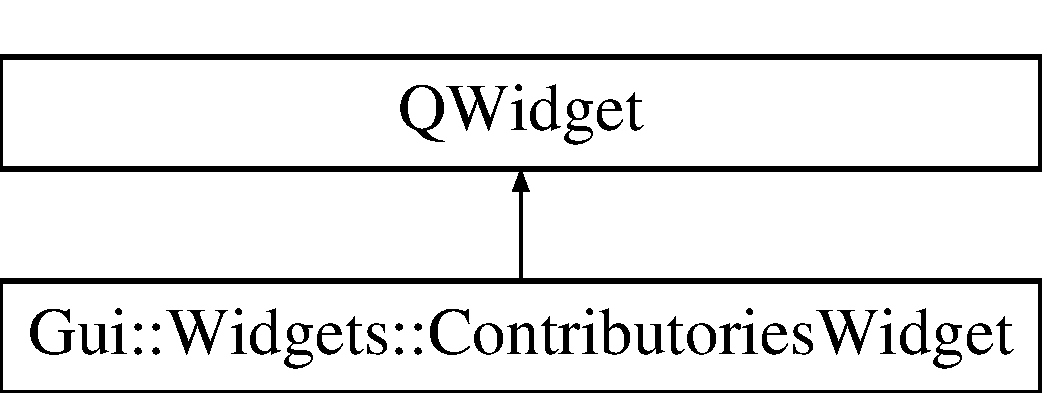
\includegraphics[height=2.000000cm]{dc/da3/classGui_1_1Widgets_1_1ContributoriesWidget}
\end{center}
\end{figure}
\subsection*{Public Slots}
\begin{DoxyCompactItemize}
\item 
\hypertarget{classGui_1_1Widgets_1_1ContributoriesWidget_a756c0d1076fad1a3805975343e66a1de}{void \hyperlink{classGui_1_1Widgets_1_1ContributoriesWidget_a756c0d1076fad1a3805975343e66a1de}{add} (void)}\label{classGui_1_1Widgets_1_1ContributoriesWidget_a756c0d1076fad1a3805975343e66a1de}

\begin{DoxyCompactList}\small\item\em \hyperlink{classGui_1_1Widgets_1_1ContributoriesWidget_ae61498391d4aaf199bed8183961d515c}{Contributories\-Widget\-::add} Add a new empty contributory. \end{DoxyCompactList}\item 
\hypertarget{classGui_1_1Widgets_1_1ContributoriesWidget_a35895ad0b9c497263f633680288b414e}{void \hyperlink{classGui_1_1Widgets_1_1ContributoriesWidget_a35895ad0b9c497263f633680288b414e}{remove} (void)}\label{classGui_1_1Widgets_1_1ContributoriesWidget_a35895ad0b9c497263f633680288b414e}

\begin{DoxyCompactList}\small\item\em \hyperlink{classGui_1_1Widgets_1_1ContributoriesWidget_a35895ad0b9c497263f633680288b414e}{Contributories\-Widget\-::remove} Remove the current contributory. \end{DoxyCompactList}\item 
void \hyperlink{classGui_1_1Widgets_1_1ContributoriesWidget_afaa982bf1f4b77fd3bf55be0c83c4056}{add\-Project} (Q\-Pair$<$ \hyperlink{classModels_1_1Project}{Project} $\ast$, \hyperlink{classModels_1_1Rate}{Rate} $>$ $\ast$p=0)
\begin{DoxyCompactList}\small\item\em \hyperlink{classGui_1_1Widgets_1_1ContributoriesWidget_afaa982bf1f4b77fd3bf55be0c83c4056}{Contributories\-Widget\-::add\-Project} Add a Projet and it rate {\itshape p} \end{DoxyCompactList}\item 
\hypertarget{classGui_1_1Widgets_1_1ContributoriesWidget_ad907c5827c4e1ee3b82adbe6f2f77309}{void \hyperlink{classGui_1_1Widgets_1_1ContributoriesWidget_ad907c5827c4e1ee3b82adbe6f2f77309}{remove\-Project} (void)}\label{classGui_1_1Widgets_1_1ContributoriesWidget_ad907c5827c4e1ee3b82adbe6f2f77309}

\begin{DoxyCompactList}\small\item\em \hyperlink{classGui_1_1Widgets_1_1ContributoriesWidget_ad907c5827c4e1ee3b82adbe6f2f77309}{Contributories\-Widget\-::remove\-Project} Remove the current Project. \end{DoxyCompactList}\item 
\hypertarget{classGui_1_1Widgets_1_1ContributoriesWidget_a5a4be90c82f8b6d0b0e3b7a658a488ee}{void \hyperlink{classGui_1_1Widgets_1_1ContributoriesWidget_a5a4be90c82f8b6d0b0e3b7a658a488ee}{change\-Project} (void)}\label{classGui_1_1Widgets_1_1ContributoriesWidget_a5a4be90c82f8b6d0b0e3b7a658a488ee}

\begin{DoxyCompactList}\small\item\em \hyperlink{classGui_1_1Widgets_1_1ContributoriesWidget_a5a4be90c82f8b6d0b0e3b7a658a488ee}{Contributories\-Widget\-::change\-Project} Change the current Project. \end{DoxyCompactList}\item 
\hypertarget{classGui_1_1Widgets_1_1ContributoriesWidget_acb1cc99ae6f72205394d7b52f0a5f20d}{void \hyperlink{classGui_1_1Widgets_1_1ContributoriesWidget_acb1cc99ae6f72205394d7b52f0a5f20d}{editing} (void)}\label{classGui_1_1Widgets_1_1ContributoriesWidget_acb1cc99ae6f72205394d7b52f0a5f20d}

\begin{DoxyCompactList}\small\item\em \hyperlink{classGui_1_1Widgets_1_1ContributoriesWidget_acb1cc99ae6f72205394d7b52f0a5f20d}{Contributories\-Widget\-::editing} Remove the current Project in the combobox not used. \end{DoxyCompactList}\item 
\hypertarget{classGui_1_1Widgets_1_1ContributoriesWidget_a5231cbde89d73ccdbb734e6aee0cb3ff}{void \hyperlink{classGui_1_1Widgets_1_1ContributoriesWidget_a5231cbde89d73ccdbb734e6aee0cb3ff}{update\-Ui} (void)}\label{classGui_1_1Widgets_1_1ContributoriesWidget_a5231cbde89d73ccdbb734e6aee0cb3ff}

\begin{DoxyCompactList}\small\item\em \hyperlink{classGui_1_1Widgets_1_1ContributoriesWidget_a5231cbde89d73ccdbb734e6aee0cb3ff}{Contributories\-Widget\-::update\-Ui} Update the User Interface. \end{DoxyCompactList}\item 
\hypertarget{classGui_1_1Widgets_1_1ContributoriesWidget_ad6c925eaf605e1b0382b0ec00eac5abf}{void \hyperlink{classGui_1_1Widgets_1_1ContributoriesWidget_ad6c925eaf605e1b0382b0ec00eac5abf}{update\-Price} (void)}\label{classGui_1_1Widgets_1_1ContributoriesWidget_ad6c925eaf605e1b0382b0ec00eac5abf}

\begin{DoxyCompactList}\small\item\em \hyperlink{classGui_1_1Widgets_1_1ContributoriesWidget_ad6c925eaf605e1b0382b0ec00eac5abf}{Contributories\-Widget\-::update\-Price} Update total price. \end{DoxyCompactList}\end{DoxyCompactItemize}
\subsection*{Signals}
\begin{DoxyCompactItemize}
\item 
\hypertarget{classGui_1_1Widgets_1_1ContributoriesWidget_a510bfd755cf271fd10b63cf68284cd02}{void \hyperlink{classGui_1_1Widgets_1_1ContributoriesWidget_a510bfd755cf271fd10b63cf68284cd02}{contributory\-Changed} ()}\label{classGui_1_1Widgets_1_1ContributoriesWidget_a510bfd755cf271fd10b63cf68284cd02}

\begin{DoxyCompactList}\small\item\em \hyperlink{classGui_1_1Widgets_1_1ContributoriesWidget_a510bfd755cf271fd10b63cf68284cd02}{Contributories\-Widget\-::contributory\-Changed} Signal that a contributory has changed. \end{DoxyCompactList}\end{DoxyCompactItemize}
\subsection*{Public Member Functions}
\begin{DoxyCompactItemize}
\item 
\hyperlink{classGui_1_1Widgets_1_1ContributoriesWidget_a5517afc134491eb118b9d183e94476bc}{Contributories\-Widget} (Q\-Shared\-Pointer$<$ \hyperlink{classModels_1_1Customer}{Customer} $>$ c, Q\-Widget $\ast$parent=0)
\begin{DoxyCompactList}\small\item\em \hyperlink{classGui_1_1Widgets_1_1ContributoriesWidget_a5517afc134491eb118b9d183e94476bc}{Contributories\-Widget\-::\-Contributories\-Widget} Construct a \hyperlink{classGui_1_1Widgets_1_1ContributoriesWidget}{Contributories\-Widget}. \end{DoxyCompactList}\item 
\hyperlink{classModels_1_1ContributoriesList}{Contributories\-List} $\ast$ \hyperlink{classGui_1_1Widgets_1_1ContributoriesWidget_a72c0f4a49aaafdf045154bafb1e76049}{get\-Contributories} () const 
\begin{DoxyCompactList}\small\item\em \hyperlink{classGui_1_1Widgets_1_1ContributoriesWidget_a72c0f4a49aaafdf045154bafb1e76049}{Contributories\-Widget\-::get\-Contributories} Get contributories List. \end{DoxyCompactList}\item 
int \hyperlink{classGui_1_1Widgets_1_1ContributoriesWidget_a7c9f1bfcac92d4813f1d43b46319042b}{count} ()
\begin{DoxyCompactList}\small\item\em \hyperlink{classGui_1_1Widgets_1_1ContributoriesWidget_a7c9f1bfcac92d4813f1d43b46319042b}{Contributories\-Widget\-::count} Numbers of contributories. \end{DoxyCompactList}\item 
void \hyperlink{classGui_1_1Widgets_1_1ContributoriesWidget_ae61498391d4aaf199bed8183961d515c}{add} (\hyperlink{classModels_1_1ContributoriesList}{Contributories\-List} \&list)
\begin{DoxyCompactList}\small\item\em \hyperlink{classGui_1_1Widgets_1_1ContributoriesWidget_ae61498391d4aaf199bed8183961d515c}{Contributories\-Widget\-::add} Add contributorieslist {\itshape list} in the model. \end{DoxyCompactList}\end{DoxyCompactItemize}


\subsection{Detailed Description}
The \hyperlink{classGui_1_1Widgets_1_1ContributoriesWidget}{Contributories\-Widget} class Widget of Contributories. 

\subsection{Constructor \& Destructor Documentation}
\hypertarget{classGui_1_1Widgets_1_1ContributoriesWidget_a5517afc134491eb118b9d183e94476bc}{\index{Gui\-::\-Widgets\-::\-Contributories\-Widget@{Gui\-::\-Widgets\-::\-Contributories\-Widget}!Contributories\-Widget@{Contributories\-Widget}}
\index{Contributories\-Widget@{Contributories\-Widget}!Gui::Widgets::ContributoriesWidget@{Gui\-::\-Widgets\-::\-Contributories\-Widget}}
\subsubsection[{Contributories\-Widget}]{\setlength{\rightskip}{0pt plus 5cm}Gui\-::\-Widgets\-::\-Contributories\-Widget\-::\-Contributories\-Widget (
\begin{DoxyParamCaption}
\item[{Q\-Shared\-Pointer$<$ {\bf Customer} $>$}]{c, }
\item[{Q\-Widget $\ast$}]{parent = {\ttfamily 0}}
\end{DoxyParamCaption}
)\hspace{0.3cm}{\ttfamily [explicit]}}}\label{classGui_1_1Widgets_1_1ContributoriesWidget_a5517afc134491eb118b9d183e94476bc}


\hyperlink{classGui_1_1Widgets_1_1ContributoriesWidget_a5517afc134491eb118b9d183e94476bc}{Contributories\-Widget\-::\-Contributories\-Widget} Construct a \hyperlink{classGui_1_1Widgets_1_1ContributoriesWidget}{Contributories\-Widget}. 


\begin{DoxyParams}{Parameters}
{\em c} & Customer \\
\hline
{\em parent} & Widget parent \\
\hline
\end{DoxyParams}


\subsection{Member Function Documentation}
\hypertarget{classGui_1_1Widgets_1_1ContributoriesWidget_ae61498391d4aaf199bed8183961d515c}{\index{Gui\-::\-Widgets\-::\-Contributories\-Widget@{Gui\-::\-Widgets\-::\-Contributories\-Widget}!add@{add}}
\index{add@{add}!Gui::Widgets::ContributoriesWidget@{Gui\-::\-Widgets\-::\-Contributories\-Widget}}
\subsubsection[{add}]{\setlength{\rightskip}{0pt plus 5cm}void Gui\-::\-Widgets\-::\-Contributories\-Widget\-::add (
\begin{DoxyParamCaption}
\item[{{\bf Contributories\-List} \&}]{list}
\end{DoxyParamCaption}
)}}\label{classGui_1_1Widgets_1_1ContributoriesWidget_ae61498391d4aaf199bed8183961d515c}


\hyperlink{classGui_1_1Widgets_1_1ContributoriesWidget_ae61498391d4aaf199bed8183961d515c}{Contributories\-Widget\-::add} Add contributorieslist {\itshape list} in the model. 


\begin{DoxyParams}{Parameters}
{\em list} & the {\bfseries Contributories\-List} \\
\hline
\end{DoxyParams}
\hypertarget{classGui_1_1Widgets_1_1ContributoriesWidget_afaa982bf1f4b77fd3bf55be0c83c4056}{\index{Gui\-::\-Widgets\-::\-Contributories\-Widget@{Gui\-::\-Widgets\-::\-Contributories\-Widget}!add\-Project@{add\-Project}}
\index{add\-Project@{add\-Project}!Gui::Widgets::ContributoriesWidget@{Gui\-::\-Widgets\-::\-Contributories\-Widget}}
\subsubsection[{add\-Project}]{\setlength{\rightskip}{0pt plus 5cm}void Gui\-::\-Widgets\-::\-Contributories\-Widget\-::add\-Project (
\begin{DoxyParamCaption}
\item[{Q\-Pair$<$ {\bf Project} $\ast$, {\bf Rate} $>$ $\ast$}]{p = {\ttfamily 0}}
\end{DoxyParamCaption}
)\hspace{0.3cm}{\ttfamily [slot]}}}\label{classGui_1_1Widgets_1_1ContributoriesWidget_afaa982bf1f4b77fd3bf55be0c83c4056}


\hyperlink{classGui_1_1Widgets_1_1ContributoriesWidget_afaa982bf1f4b77fd3bf55be0c83c4056}{Contributories\-Widget\-::add\-Project} Add a Projet and it rate {\itshape p} 


\begin{DoxyParams}{Parameters}
{\em p} & Rate linked to Project \\
\hline
\end{DoxyParams}
\hypertarget{classGui_1_1Widgets_1_1ContributoriesWidget_a7c9f1bfcac92d4813f1d43b46319042b}{\index{Gui\-::\-Widgets\-::\-Contributories\-Widget@{Gui\-::\-Widgets\-::\-Contributories\-Widget}!count@{count}}
\index{count@{count}!Gui::Widgets::ContributoriesWidget@{Gui\-::\-Widgets\-::\-Contributories\-Widget}}
\subsubsection[{count}]{\setlength{\rightskip}{0pt plus 5cm}int Gui\-::\-Widgets\-::\-Contributories\-Widget\-::count (
\begin{DoxyParamCaption}
{}
\end{DoxyParamCaption}
)}}\label{classGui_1_1Widgets_1_1ContributoriesWidget_a7c9f1bfcac92d4813f1d43b46319042b}


\hyperlink{classGui_1_1Widgets_1_1ContributoriesWidget_a7c9f1bfcac92d4813f1d43b46319042b}{Contributories\-Widget\-::count} Numbers of contributories. 

\begin{DoxyReturn}{Returns}
Numbers of contributories 
\end{DoxyReturn}
\hypertarget{classGui_1_1Widgets_1_1ContributoriesWidget_a72c0f4a49aaafdf045154bafb1e76049}{\index{Gui\-::\-Widgets\-::\-Contributories\-Widget@{Gui\-::\-Widgets\-::\-Contributories\-Widget}!get\-Contributories@{get\-Contributories}}
\index{get\-Contributories@{get\-Contributories}!Gui::Widgets::ContributoriesWidget@{Gui\-::\-Widgets\-::\-Contributories\-Widget}}
\subsubsection[{get\-Contributories}]{\setlength{\rightskip}{0pt plus 5cm}{\bf Contributories\-List} $\ast$ Gui\-::\-Widgets\-::\-Contributories\-Widget\-::get\-Contributories (
\begin{DoxyParamCaption}
{}
\end{DoxyParamCaption}
) const}}\label{classGui_1_1Widgets_1_1ContributoriesWidget_a72c0f4a49aaafdf045154bafb1e76049}


\hyperlink{classGui_1_1Widgets_1_1ContributoriesWidget_a72c0f4a49aaafdf045154bafb1e76049}{Contributories\-Widget\-::get\-Contributories} Get contributories List. 

\begin{DoxyReturn}{Returns}
Contributories\-List 
\end{DoxyReturn}


The documentation for this class was generated from the following files\-:\begin{DoxyCompactItemize}
\item 
/home/travis/build/\-F\-A\-C\-T-\/\-Team/\-Fact\-Dev/src/gui/widgets/contributorieswidget.\-h\item 
/home/travis/build/\-F\-A\-C\-T-\/\-Team/\-Fact\-Dev/src/gui/widgets/contributorieswidget.\-cpp\end{DoxyCompactItemize}

\hypertarget{classModels_1_1Contributory}{}\section{Models\+:\+:Contributory Class Reference}
\label{classModels_1_1Contributory}\index{Models\+::\+Contributory@{Models\+::\+Contributory}}


The \hyperlink{classModels_1_1Unit}{Unit} enum Unity of work \+: hour or day.  




{\ttfamily \#include $<$contributory.\+h$>$}

Inheritance diagram for Models\+:\+:Contributory\+:\begin{figure}[H]
\begin{center}
\leavevmode
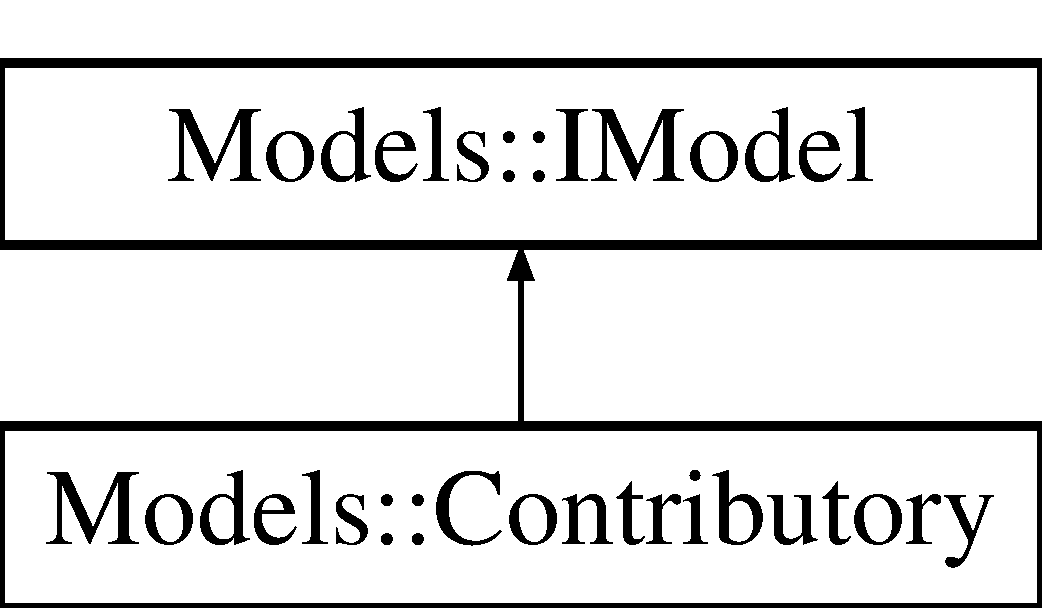
\includegraphics[height=2.000000cm]{d5/dd1/classModels_1_1Contributory}
\end{center}
\end{figure}
\subsection*{Public Member Functions}
\begin{DoxyCompactItemize}
\item 
\hypertarget{classModels_1_1Contributory_a82c2a30e60a256099f25c424337d5aa0}{}\hyperlink{classModels_1_1Contributory_a82c2a30e60a256099f25c424337d5aa0}{Contributory} ()\label{classModels_1_1Contributory_a82c2a30e60a256099f25c424337d5aa0}

\begin{DoxyCompactList}\small\item\em \hyperlink{classModels_1_1Contributory_a82c2a30e60a256099f25c424337d5aa0}{Contributory\+::\+Contributory} Contruct a \hyperlink{classModels_1_1Contributory}{Contributory}. \end{DoxyCompactList}\item 
\hyperlink{classModels_1_1Contributory_acbece77d876ca9d49d9fec868a74be5f}{Contributory} (int id)
\begin{DoxyCompactList}\small\item\em \hyperlink{classModels_1_1Contributory_a82c2a30e60a256099f25c424337d5aa0}{Contributory\+::\+Contributory} Contruct a \hyperlink{classModels_1_1Contributory}{Contributory} and get data in database. \end{DoxyCompactList}\item 
\hypertarget{classModels_1_1Contributory_a27d9ade910eab64b0e1135bb25ce0308}{}\hyperlink{classModels_1_1Contributory_a27d9ade910eab64b0e1135bb25ce0308}{$\sim$\+Contributory} ()\label{classModels_1_1Contributory_a27d9ade910eab64b0e1135bb25ce0308}

\begin{DoxyCompactList}\small\item\em Destroy an contributory object. \end{DoxyCompactList}\item 
\hypertarget{classModels_1_1Contributory_a2d89036a02bd2828ff76d047338f61ba}{}void \hyperlink{classModels_1_1Contributory_a2d89036a02bd2828ff76d047338f61ba}{commit} ()\label{classModels_1_1Contributory_a2d89036a02bd2828ff76d047338f61ba}

\begin{DoxyCompactList}\small\item\em \hyperlink{classModels_1_1Contributory_a2d89036a02bd2828ff76d047338f61ba}{Contributory\+::commit} Update or insert a contributory to the database. \end{DoxyCompactList}\item 
void \hyperlink{classModels_1_1Contributory_a40248b5853045eb46412396513f36b06}{hydrat} (int id)
\begin{DoxyCompactList}\small\item\em \hyperlink{classModels_1_1Contributory_a40248b5853045eb46412396513f36b06}{Contributory\+::hydrat} Get data about the \hyperlink{classModels_1_1Contributory}{Contributory} which is specified by the identify {\itshape id} \end{DoxyCompactList}\item 
\hypertarget{classModels_1_1Contributory_ab9971d7867516b488095e63e1179eac8}{}void \hyperlink{classModels_1_1Contributory_ab9971d7867516b488095e63e1179eac8}{remove} ()\label{classModels_1_1Contributory_ab9971d7867516b488095e63e1179eac8}

\begin{DoxyCompactList}\small\item\em \hyperlink{classModels_1_1Contributory_ab9971d7867516b488095e63e1179eac8}{Contributory\+::remove} Remove the current \hyperlink{classModels_1_1Contributory}{Contributory}. \end{DoxyCompactList}\item 
double \hyperlink{classModels_1_1Contributory_ac8eb5c2589dd05bba5b51ac190ecd778}{get\+Price} (const bool paied=false)
\begin{DoxyCompactList}\small\item\em get\+Price Return the price of a contributory \end{DoxyCompactList}\item 
double \hyperlink{classModels_1_1Contributory_aa6f3e9018846a83d192b8fb427fe0481}{get\+Sum\+Quantity} ()
\begin{DoxyCompactList}\small\item\em \hyperlink{classModels_1_1ContributoriesList_af9b3b1b703cebeef552d058999ffcc4c}{Contributories\+List\+::get\+Sum\+Quantity} Return the sum of quantity (number of hours) of the Contributories. \end{DoxyCompactList}\item 
Q\+Variant\+Hash \hyperlink{classModels_1_1Contributory_a692f563f0428866441ea8bc2b9e772ca}{get\+Data\+Map} ()
\begin{DoxyCompactList}\small\item\em get\+Data\+Map Get all data of model with a Hash\+Map key/value \end{DoxyCompactList}\item 
\hyperlink{classModels_1_1Project}{Project} $\ast$ \hyperlink{classModels_1_1Contributory_a49379aeb4de2376d5a2aaf10f54daf05}{get\+Project} () const 
\begin{DoxyCompactList}\small\item\em \hyperlink{classModels_1_1Contributory_a49379aeb4de2376d5a2aaf10f54daf05}{Contributory\+::get\+Project} Return the project linked to this \hyperlink{classModels_1_1Contributory}{Contributory}. \end{DoxyCompactList}\item 
void \hyperlink{classModels_1_1Contributory_a4478894daf317068856b707491d03555}{set\+Project} (\hyperlink{classModels_1_1Project}{Project} $\ast$id)
\begin{DoxyCompactList}\small\item\em \hyperlink{classModels_1_1Contributory_a4478894daf317068856b707491d03555}{Contributory\+::set\+Project} Modify the identify {\itshape id} of the \hyperlink{classModels_1_1Project}{Project} linked to this \hyperlink{classModels_1_1Contributory}{Contributory}. \end{DoxyCompactList}\item 
double \hyperlink{classModels_1_1Contributory_a7c5fdd6e53641ae441054ebe7393f59d}{get\+Quantity} () const 
\begin{DoxyCompactList}\small\item\em get\+Nb\+Hours Number of work hour of a contributory \end{DoxyCompactList}\item 
void \hyperlink{classModels_1_1Contributory_afe02bdd167c6aed02c81a6e684293e99}{set\+Quantity} (double value)
\begin{DoxyCompactList}\small\item\em set\+Nb\+Hours Change nb\+Hours \end{DoxyCompactList}\item 
Q\+String \hyperlink{classModels_1_1Contributory_ae2b936f2fb1ccad2009eae9b5d12fc02}{get\+Description} () const 
\begin{DoxyCompactList}\small\item\em get\+Description Description of a contributory \end{DoxyCompactList}\item 
void \hyperlink{classModels_1_1Contributory_a12d4199fa7175c0b43f62eddf7c3d69e}{set\+Description} (const Q\+String \&\hyperlink{classModels_1_1Contributory_ae2b936f2fb1ccad2009eae9b5d12fc02}{get\+Description})
\begin{DoxyCompactList}\small\item\em set\+Description Change the contributory description \end{DoxyCompactList}\item 
bool \hyperlink{classModels_1_1Contributory_ad49c8b9cdf7254069e07f2238b42c8f3}{operator==} (const \hyperlink{classModels_1_1Contributory}{Contributory} \&c)
\begin{DoxyCompactList}\small\item\em operator == define the operator \char`\"{}==\char`\"{} to compare two {\bfseries \hyperlink{classModels_1_1Contributory}{Contributory}} \end{DoxyCompactList}\item 
bool \hyperlink{classModels_1_1Contributory_a0808e6453b222f62d3288361dcb56d16}{operator!=} (const \hyperlink{classModels_1_1Contributory}{Contributory} \&c)
\begin{DoxyCompactList}\small\item\em operator != define the operator \char`\"{}!=\char`\"{} to compare two {\bfseries \hyperlink{classModels_1_1Contributory}{Contributory}} \end{DoxyCompactList}\item 
Q\+String \hyperlink{classModels_1_1Contributory_abcd8dce3a913d558b73f17f16d5beb7a}{get\+Long\+Description} () const 
\begin{DoxyCompactList}\small\item\em get\+Long\+Description A contributory has a long description \+: display in tex appendix \end{DoxyCompactList}\item 
void \hyperlink{classModels_1_1Contributory_a40023cef80233eaa814d7bb41d668322}{set\+Long\+Description} (const Q\+String \&\hyperlink{classModels_1_1Contributory_abcd8dce3a913d558b73f17f16d5beb7a}{get\+Long\+Description})
\begin{DoxyCompactList}\small\item\em set\+Long\+Description Change the long description \end{DoxyCompactList}\item 
\hyperlink{classModels_1_1Unit}{Unit} \hyperlink{classModels_1_1Contributory_aa89a7587555a6ec768638e0c21d17450}{get\+Unit} () const 
\begin{DoxyCompactList}\small\item\em get\+Unit Return the unit (hour or day) of contributory \end{DoxyCompactList}\item 
void \hyperlink{classModels_1_1Contributory_a257273fe7acbd73c885d1c0fdddbb95e}{set\+Unit} (const \hyperlink{classModels_1_1Unit}{Unit} \&value)
\begin{DoxyCompactList}\small\item\em set\+Unit Change the unit \end{DoxyCompactList}\item 
double \hyperlink{classModels_1_1Contributory_aa6e1d43e7ca2e5e09bf6f1b65f577a0b}{get\+Hourly\+Rate} () const 
\begin{DoxyCompactList}\small\item\em get\+Hourly\+Rate Hourly rate for this contributory \end{DoxyCompactList}\item 
void \hyperlink{classModels_1_1Contributory_a08adb4281ec3a57c839290d01b1f41e5}{set\+Hourly\+Rate} (double value)
\begin{DoxyCompactList}\small\item\em set\+Hourly\+Rate Change the hourly rate for this contributory \end{DoxyCompactList}\end{DoxyCompactItemize}
\subsection*{Additional Inherited Members}


\subsection{Detailed Description}
The \hyperlink{classModels_1_1Unit}{Unit} enum Unity of work \+: hour or day. 

\begin{DoxyAuthor}{Author}
The \hyperlink{classModels_1_1Contributory}{Contributory} class 
\end{DoxyAuthor}


\subsection{Constructor \& Destructor Documentation}
\hypertarget{classModels_1_1Contributory_acbece77d876ca9d49d9fec868a74be5f}{}\index{Models\+::\+Contributory@{Models\+::\+Contributory}!Contributory@{Contributory}}
\index{Contributory@{Contributory}!Models\+::\+Contributory@{Models\+::\+Contributory}}
\subsubsection[{Contributory}]{\setlength{\rightskip}{0pt plus 5cm}Models\+::\+Contributory\+::\+Contributory (
\begin{DoxyParamCaption}
\item[{int}]{id}
\end{DoxyParamCaption}
)}\label{classModels_1_1Contributory_acbece77d876ca9d49d9fec868a74be5f}


\hyperlink{classModels_1_1Contributory_a82c2a30e60a256099f25c424337d5aa0}{Contributory\+::\+Contributory} Contruct a \hyperlink{classModels_1_1Contributory}{Contributory} and get data in database. 


\begin{DoxyParams}{Parameters}
{\em id} & \hyperlink{classModels_1_1Contributory}{Contributory}\textquotesingle{}s id \\
\hline
\end{DoxyParams}


\subsection{Member Function Documentation}
\hypertarget{classModels_1_1Contributory_a692f563f0428866441ea8bc2b9e772ca}{}\index{Models\+::\+Contributory@{Models\+::\+Contributory}!get\+Data\+Map@{get\+Data\+Map}}
\index{get\+Data\+Map@{get\+Data\+Map}!Models\+::\+Contributory@{Models\+::\+Contributory}}
\subsubsection[{get\+Data\+Map}]{\setlength{\rightskip}{0pt plus 5cm}Q\+Variant\+Hash Models\+::\+Contributory\+::get\+Data\+Map (
\begin{DoxyParamCaption}
{}
\end{DoxyParamCaption}
)\hspace{0.3cm}{\ttfamily [virtual]}}\label{classModels_1_1Contributory_a692f563f0428866441ea8bc2b9e772ca}


get\+Data\+Map Get all data of model with a Hash\+Map key/value 

\begin{DoxyReturn}{Returns}
Model\textquotesingle{}s data 
\end{DoxyReturn}


Implements \hyperlink{classModels_1_1IModel_a9851b0f296aac58353edff22af11cf3c}{Models\+::\+I\+Model}.

\hypertarget{classModels_1_1Contributory_ae2b936f2fb1ccad2009eae9b5d12fc02}{}\index{Models\+::\+Contributory@{Models\+::\+Contributory}!get\+Description@{get\+Description}}
\index{get\+Description@{get\+Description}!Models\+::\+Contributory@{Models\+::\+Contributory}}
\subsubsection[{get\+Description}]{\setlength{\rightskip}{0pt plus 5cm}Q\+String Models\+::\+Contributory\+::get\+Description (
\begin{DoxyParamCaption}
{}
\end{DoxyParamCaption}
) const}\label{classModels_1_1Contributory_ae2b936f2fb1ccad2009eae9b5d12fc02}


get\+Description Description of a contributory 

\begin{DoxyReturn}{Returns}
The description 
\end{DoxyReturn}
\hypertarget{classModels_1_1Contributory_aa6e1d43e7ca2e5e09bf6f1b65f577a0b}{}\index{Models\+::\+Contributory@{Models\+::\+Contributory}!get\+Hourly\+Rate@{get\+Hourly\+Rate}}
\index{get\+Hourly\+Rate@{get\+Hourly\+Rate}!Models\+::\+Contributory@{Models\+::\+Contributory}}
\subsubsection[{get\+Hourly\+Rate}]{\setlength{\rightskip}{0pt plus 5cm}double Models\+::\+Contributory\+::get\+Hourly\+Rate (
\begin{DoxyParamCaption}
{}
\end{DoxyParamCaption}
) const}\label{classModels_1_1Contributory_aa6e1d43e7ca2e5e09bf6f1b65f577a0b}


get\+Hourly\+Rate Hourly rate for this contributory 

\begin{DoxyReturn}{Returns}
The hourly rate 
\end{DoxyReturn}
\hypertarget{classModels_1_1Contributory_abcd8dce3a913d558b73f17f16d5beb7a}{}\index{Models\+::\+Contributory@{Models\+::\+Contributory}!get\+Long\+Description@{get\+Long\+Description}}
\index{get\+Long\+Description@{get\+Long\+Description}!Models\+::\+Contributory@{Models\+::\+Contributory}}
\subsubsection[{get\+Long\+Description}]{\setlength{\rightskip}{0pt plus 5cm}Q\+String Models\+::\+Contributory\+::get\+Long\+Description (
\begin{DoxyParamCaption}
{}
\end{DoxyParamCaption}
) const}\label{classModels_1_1Contributory_abcd8dce3a913d558b73f17f16d5beb7a}


get\+Long\+Description A contributory has a long description \+: display in tex appendix 

\begin{DoxyReturn}{Returns}
The long description 
\end{DoxyReturn}
\hypertarget{classModels_1_1Contributory_ac8eb5c2589dd05bba5b51ac190ecd778}{}\index{Models\+::\+Contributory@{Models\+::\+Contributory}!get\+Price@{get\+Price}}
\index{get\+Price@{get\+Price}!Models\+::\+Contributory@{Models\+::\+Contributory}}
\subsubsection[{get\+Price}]{\setlength{\rightskip}{0pt plus 5cm}double Models\+::\+Contributory\+::get\+Price (
\begin{DoxyParamCaption}
\item[{const bool}]{paied = {\ttfamily false}}
\end{DoxyParamCaption}
)\hspace{0.3cm}{\ttfamily [virtual]}}\label{classModels_1_1Contributory_ac8eb5c2589dd05bba5b51ac190ecd778}


get\+Price Return the price of a contributory 

\begin{DoxyReturn}{Returns}
The price 
\end{DoxyReturn}


Implements \hyperlink{classModels_1_1Calculable_a5267ee09fc9284063a9fc874b4cc68dc}{Models\+::\+Calculable}.

\hypertarget{classModels_1_1Contributory_a49379aeb4de2376d5a2aaf10f54daf05}{}\index{Models\+::\+Contributory@{Models\+::\+Contributory}!get\+Project@{get\+Project}}
\index{get\+Project@{get\+Project}!Models\+::\+Contributory@{Models\+::\+Contributory}}
\subsubsection[{get\+Project}]{\setlength{\rightskip}{0pt plus 5cm}{\bf Project} $\ast$ Models\+::\+Contributory\+::get\+Project (
\begin{DoxyParamCaption}
{}
\end{DoxyParamCaption}
) const}\label{classModels_1_1Contributory_a49379aeb4de2376d5a2aaf10f54daf05}


\hyperlink{classModels_1_1Contributory_a49379aeb4de2376d5a2aaf10f54daf05}{Contributory\+::get\+Project} Return the project linked to this \hyperlink{classModels_1_1Contributory}{Contributory}. 

\begin{DoxyReturn}{Returns}
\hyperlink{classModels_1_1Project}{Project} linked to this \hyperlink{classModels_1_1Contributory}{Contributory} 
\end{DoxyReturn}
\hypertarget{classModels_1_1Contributory_a7c5fdd6e53641ae441054ebe7393f59d}{}\index{Models\+::\+Contributory@{Models\+::\+Contributory}!get\+Quantity@{get\+Quantity}}
\index{get\+Quantity@{get\+Quantity}!Models\+::\+Contributory@{Models\+::\+Contributory}}
\subsubsection[{get\+Quantity}]{\setlength{\rightskip}{0pt plus 5cm}double Models\+::\+Contributory\+::get\+Quantity (
\begin{DoxyParamCaption}
{}
\end{DoxyParamCaption}
) const}\label{classModels_1_1Contributory_a7c5fdd6e53641ae441054ebe7393f59d}


get\+Nb\+Hours Number of work hour of a contributory 

\begin{DoxyReturn}{Returns}
Then number of hours 
\end{DoxyReturn}
\hypertarget{classModels_1_1Contributory_aa6f3e9018846a83d192b8fb427fe0481}{}\index{Models\+::\+Contributory@{Models\+::\+Contributory}!get\+Sum\+Quantity@{get\+Sum\+Quantity}}
\index{get\+Sum\+Quantity@{get\+Sum\+Quantity}!Models\+::\+Contributory@{Models\+::\+Contributory}}
\subsubsection[{get\+Sum\+Quantity}]{\setlength{\rightskip}{0pt plus 5cm}double Models\+::\+Contributory\+::get\+Sum\+Quantity (
\begin{DoxyParamCaption}
{}
\end{DoxyParamCaption}
)\hspace{0.3cm}{\ttfamily [virtual]}}\label{classModels_1_1Contributory_aa6f3e9018846a83d192b8fb427fe0481}


\hyperlink{classModels_1_1ContributoriesList_af9b3b1b703cebeef552d058999ffcc4c}{Contributories\+List\+::get\+Sum\+Quantity} Return the sum of quantity (number of hours) of the Contributories. 

\begin{DoxyReturn}{Returns}
sum of quantity in hours 
\end{DoxyReturn}


Implements \hyperlink{classModels_1_1Calculable_a4f9d590b39bd1f0d9e026ac86f1fada1}{Models\+::\+Calculable}.

\hypertarget{classModels_1_1Contributory_aa89a7587555a6ec768638e0c21d17450}{}\index{Models\+::\+Contributory@{Models\+::\+Contributory}!get\+Unit@{get\+Unit}}
\index{get\+Unit@{get\+Unit}!Models\+::\+Contributory@{Models\+::\+Contributory}}
\subsubsection[{get\+Unit}]{\setlength{\rightskip}{0pt plus 5cm}{\bf Unit} Models\+::\+Contributory\+::get\+Unit (
\begin{DoxyParamCaption}
{}
\end{DoxyParamCaption}
) const}\label{classModels_1_1Contributory_aa89a7587555a6ec768638e0c21d17450}


get\+Unit Return the unit (hour or day) of contributory 

\begin{DoxyReturn}{Returns}
The unit 
\end{DoxyReturn}
\hypertarget{classModels_1_1Contributory_a40248b5853045eb46412396513f36b06}{}\index{Models\+::\+Contributory@{Models\+::\+Contributory}!hydrat@{hydrat}}
\index{hydrat@{hydrat}!Models\+::\+Contributory@{Models\+::\+Contributory}}
\subsubsection[{hydrat}]{\setlength{\rightskip}{0pt plus 5cm}void Models\+::\+Contributory\+::hydrat (
\begin{DoxyParamCaption}
\item[{int}]{id}
\end{DoxyParamCaption}
)\hspace{0.3cm}{\ttfamily [virtual]}}\label{classModels_1_1Contributory_a40248b5853045eb46412396513f36b06}


\hyperlink{classModels_1_1Contributory_a40248b5853045eb46412396513f36b06}{Contributory\+::hydrat} Get data about the \hyperlink{classModels_1_1Contributory}{Contributory} which is specified by the identify {\itshape id} 


\begin{DoxyParams}{Parameters}
{\em id} & \hyperlink{classModels_1_1Contributory}{Contributory} identify \\
\hline
\end{DoxyParams}


Implements \hyperlink{classModels_1_1IModel_a7ce6def437f5e1f6a78ee1d67ca028e4}{Models\+::\+I\+Model}.

\hypertarget{classModels_1_1Contributory_a0808e6453b222f62d3288361dcb56d16}{}\index{Models\+::\+Contributory@{Models\+::\+Contributory}!operator"!=@{operator"!=}}
\index{operator"!=@{operator"!=}!Models\+::\+Contributory@{Models\+::\+Contributory}}
\subsubsection[{operator"!=}]{\setlength{\rightskip}{0pt plus 5cm}bool Models\+::\+Contributory\+::operator!= (
\begin{DoxyParamCaption}
\item[{const {\bf Contributory} \&}]{c}
\end{DoxyParamCaption}
)}\label{classModels_1_1Contributory_a0808e6453b222f62d3288361dcb56d16}


operator != define the operator \char`\"{}!=\char`\"{} to compare two {\bfseries \hyperlink{classModels_1_1Contributory}{Contributory}} 


\begin{DoxyParams}{Parameters}
{\em c} & the {\bfseries \hyperlink{classModels_1_1Contributory}{Contributory}} to compare with the current {\bfseries \hyperlink{classModels_1_1Contributory}{Contributory}} \\
\hline
\end{DoxyParams}
\begin{DoxyReturn}{Returns}
true if the {\bfseries \hyperlink{classModels_1_1Contributory}{Contributory}} are different else false 
\end{DoxyReturn}
\hypertarget{classModels_1_1Contributory_ad49c8b9cdf7254069e07f2238b42c8f3}{}\index{Models\+::\+Contributory@{Models\+::\+Contributory}!operator==@{operator==}}
\index{operator==@{operator==}!Models\+::\+Contributory@{Models\+::\+Contributory}}
\subsubsection[{operator==}]{\setlength{\rightskip}{0pt plus 5cm}bool Models\+::\+Contributory\+::operator== (
\begin{DoxyParamCaption}
\item[{const {\bf Contributory} \&}]{c}
\end{DoxyParamCaption}
)}\label{classModels_1_1Contributory_ad49c8b9cdf7254069e07f2238b42c8f3}


operator == define the operator \char`\"{}==\char`\"{} to compare two {\bfseries \hyperlink{classModels_1_1Contributory}{Contributory}} 


\begin{DoxyParams}{Parameters}
{\em c} & the {\bfseries \hyperlink{classModels_1_1Contributory}{Contributory}} to compare with the current {\bfseries \hyperlink{classModels_1_1Contributory}{Contributory}} \\
\hline
\end{DoxyParams}
\begin{DoxyReturn}{Returns}
true if the {\bfseries \hyperlink{classModels_1_1Contributory}{Contributory}} are equals else false 
\end{DoxyReturn}
\hypertarget{classModels_1_1Contributory_a12d4199fa7175c0b43f62eddf7c3d69e}{}\index{Models\+::\+Contributory@{Models\+::\+Contributory}!set\+Description@{set\+Description}}
\index{set\+Description@{set\+Description}!Models\+::\+Contributory@{Models\+::\+Contributory}}
\subsubsection[{set\+Description}]{\setlength{\rightskip}{0pt plus 5cm}void Models\+::\+Contributory\+::set\+Description (
\begin{DoxyParamCaption}
\item[{const Q\+String \&}]{get\+Description}
\end{DoxyParamCaption}
)}\label{classModels_1_1Contributory_a12d4199fa7175c0b43f62eddf7c3d69e}


set\+Description Change the contributory description 


\begin{DoxyParams}{Parameters}
{\em get\+Description} & The new description \\
\hline
\end{DoxyParams}
\hypertarget{classModels_1_1Contributory_a08adb4281ec3a57c839290d01b1f41e5}{}\index{Models\+::\+Contributory@{Models\+::\+Contributory}!set\+Hourly\+Rate@{set\+Hourly\+Rate}}
\index{set\+Hourly\+Rate@{set\+Hourly\+Rate}!Models\+::\+Contributory@{Models\+::\+Contributory}}
\subsubsection[{set\+Hourly\+Rate}]{\setlength{\rightskip}{0pt plus 5cm}void Models\+::\+Contributory\+::set\+Hourly\+Rate (
\begin{DoxyParamCaption}
\item[{double}]{value}
\end{DoxyParamCaption}
)}\label{classModels_1_1Contributory_a08adb4281ec3a57c839290d01b1f41e5}


set\+Hourly\+Rate Change the hourly rate for this contributory 


\begin{DoxyParams}{Parameters}
{\em value} & The hourly rate \\
\hline
\end{DoxyParams}
\hypertarget{classModels_1_1Contributory_a40023cef80233eaa814d7bb41d668322}{}\index{Models\+::\+Contributory@{Models\+::\+Contributory}!set\+Long\+Description@{set\+Long\+Description}}
\index{set\+Long\+Description@{set\+Long\+Description}!Models\+::\+Contributory@{Models\+::\+Contributory}}
\subsubsection[{set\+Long\+Description}]{\setlength{\rightskip}{0pt plus 5cm}void Models\+::\+Contributory\+::set\+Long\+Description (
\begin{DoxyParamCaption}
\item[{const Q\+String \&}]{get\+Long\+Description}
\end{DoxyParamCaption}
)}\label{classModels_1_1Contributory_a40023cef80233eaa814d7bb41d668322}


set\+Long\+Description Change the long description 


\begin{DoxyParams}{Parameters}
{\em get\+Long\+Description} & The new description \\
\hline
\end{DoxyParams}
\hypertarget{classModels_1_1Contributory_a4478894daf317068856b707491d03555}{}\index{Models\+::\+Contributory@{Models\+::\+Contributory}!set\+Project@{set\+Project}}
\index{set\+Project@{set\+Project}!Models\+::\+Contributory@{Models\+::\+Contributory}}
\subsubsection[{set\+Project}]{\setlength{\rightskip}{0pt plus 5cm}void Models\+::\+Contributory\+::set\+Project (
\begin{DoxyParamCaption}
\item[{{\bf Project} $\ast$}]{id}
\end{DoxyParamCaption}
)}\label{classModels_1_1Contributory_a4478894daf317068856b707491d03555}


\hyperlink{classModels_1_1Contributory_a4478894daf317068856b707491d03555}{Contributory\+::set\+Project} Modify the identify {\itshape id} of the \hyperlink{classModels_1_1Project}{Project} linked to this \hyperlink{classModels_1_1Contributory}{Contributory}. 


\begin{DoxyParams}{Parameters}
{\em id} & \hyperlink{classModels_1_1Project}{Project} Identify \\
\hline
\end{DoxyParams}
\hypertarget{classModels_1_1Contributory_afe02bdd167c6aed02c81a6e684293e99}{}\index{Models\+::\+Contributory@{Models\+::\+Contributory}!set\+Quantity@{set\+Quantity}}
\index{set\+Quantity@{set\+Quantity}!Models\+::\+Contributory@{Models\+::\+Contributory}}
\subsubsection[{set\+Quantity}]{\setlength{\rightskip}{0pt plus 5cm}void Models\+::\+Contributory\+::set\+Quantity (
\begin{DoxyParamCaption}
\item[{double}]{value}
\end{DoxyParamCaption}
)}\label{classModels_1_1Contributory_afe02bdd167c6aed02c81a6e684293e99}


set\+Nb\+Hours Change nb\+Hours 


\begin{DoxyParams}{Parameters}
{\em value} & The new value of nb\+Hours \\
\hline
\end{DoxyParams}
\hypertarget{classModels_1_1Contributory_a257273fe7acbd73c885d1c0fdddbb95e}{}\index{Models\+::\+Contributory@{Models\+::\+Contributory}!set\+Unit@{set\+Unit}}
\index{set\+Unit@{set\+Unit}!Models\+::\+Contributory@{Models\+::\+Contributory}}
\subsubsection[{set\+Unit}]{\setlength{\rightskip}{0pt plus 5cm}void Models\+::\+Contributory\+::set\+Unit (
\begin{DoxyParamCaption}
\item[{const {\bf Unit} \&}]{value}
\end{DoxyParamCaption}
)}\label{classModels_1_1Contributory_a257273fe7acbd73c885d1c0fdddbb95e}


set\+Unit Change the unit 


\begin{DoxyParams}{Parameters}
{\em value} & The new unit \\
\hline
\end{DoxyParams}


The documentation for this class was generated from the following files\+:\begin{DoxyCompactItemize}
\item 
src/models/contributory.\+h\item 
src/models/contributory.\+cpp\end{DoxyCompactItemize}

\hypertarget{classDatabase_1_1ContributoryDatabase}{\section{Database\+:\+:Contributory\+Database Class Reference}
\label{classDatabase_1_1ContributoryDatabase}\index{Database\+::\+Contributory\+Database@{Database\+::\+Contributory\+Database}}
}


The {\bfseries \hyperlink{classDatabase_1_1ContributoryDatabase}{Contributory\+Database}} class Contributory (or Quote) table database.  




{\ttfamily \#include $<$contributorydatabase.\+h$>$}

Inheritance diagram for Database\+:\+:Contributory\+Database\+:\begin{figure}[H]
\begin{center}
\leavevmode
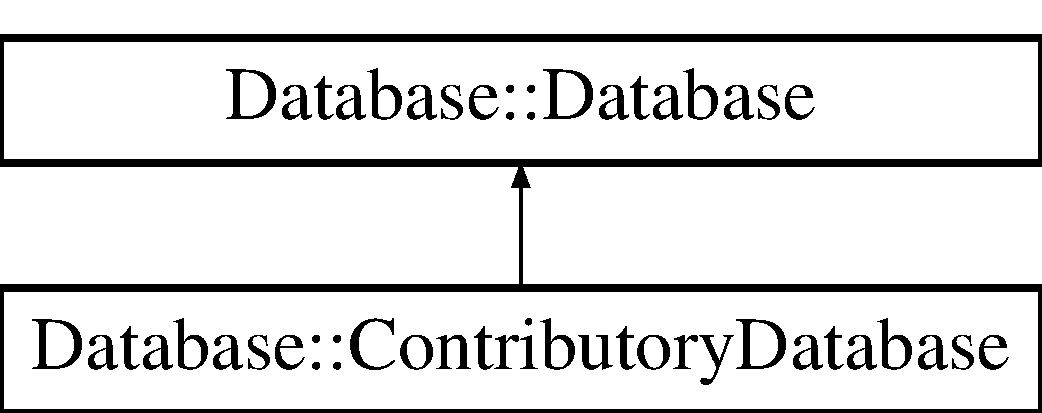
\includegraphics[height=2.000000cm]{d5/de0/classDatabase_1_1ContributoryDatabase}
\end{center}
\end{figure}
\subsection*{Public Member Functions}
\begin{DoxyCompactItemize}
\item 
\hyperlink{classModels_1_1Contributory}{Models\+::\+Contributory} $\ast$ \hyperlink{classDatabase_1_1ContributoryDatabase_afe8913f62dfb75115090650d194a7bc4}{get\+Contributory} (const int id\+Contributory)
\begin{DoxyCompactList}\small\item\em Contributory\+Database\+::get\+Customer get informations about the Contributory identified by {\itshape p\+Id} \end{DoxyCompactList}\item 
\hypertarget{classDatabase_1_1ContributoryDatabase_ad5c2a9908b0ad088eed587a16dc6fc07}{Q\+Map$<$ \hyperlink{classModels_1_1Project}{Models\+::\+Project} $\ast$, Q\+List\\*
$<$ \hyperlink{classModels_1_1Contributory}{Models\+::\+Contributory} $>$ $>$ {\bfseries get\+Contributories\+By\+Billing} (const int id\+Billing)}\label{classDatabase_1_1ContributoryDatabase_ad5c2a9908b0ad088eed587a16dc6fc07}

\item 
int \hyperlink{classDatabase_1_1ContributoryDatabase_a7612a74e10fc04a5894bf01b6917a42e}{add\+Contributory} (const \hyperlink{classModels_1_1Contributory}{Models\+::\+Contributory} \&)
\begin{DoxyCompactList}\small\item\em \hyperlink{classDatabase_1_1ContributoryDatabase_a7612a74e10fc04a5894bf01b6917a42e}{Contributory\+Database\+::add\+Contributory} Add the Contributory {\itshape p\+Contributory} to the database. \end{DoxyCompactList}\item 
\hypertarget{classDatabase_1_1ContributoryDatabase_a7f0abb17daa85b89f1a756a7ee2e482c}{void \hyperlink{classDatabase_1_1ContributoryDatabase_a7f0abb17daa85b89f1a756a7ee2e482c}{update\+Contributory} (const \hyperlink{classModels_1_1Contributory}{Models\+::\+Contributory} \&)}\label{classDatabase_1_1ContributoryDatabase_a7f0abb17daa85b89f1a756a7ee2e482c}

\begin{DoxyCompactList}\small\item\em Contributory\+Database\+::update\+Customer Update informations about the Contributory {\itshape p\+Customer} \end{DoxyCompactList}\item 
void \hyperlink{classDatabase_1_1ContributoryDatabase_aa362a76075ce095410411d7ac26bad5c}{remove\+Contributory} (const int p\+Id)
\begin{DoxyCompactList}\small\item\em Contributory\+Database\+::remove\+Customer Remove the Contributory with the id {\itshape p\+Id} \end{DoxyCompactList}\item 
\hyperlink{classModels_1_1Contributory}{Models\+::\+Contributory} $\ast$ \hyperlink{classDatabase_1_1ContributoryDatabase_af09f192038c786e0f4a2501214667cda}{get\+Contributory} (Q\+Sql\+Query \&q)
\begin{DoxyCompactList}\small\item\em get\+Contributory Obtain a contributory without new query \end{DoxyCompactList}\end{DoxyCompactItemize}
\subsection*{Static Public Member Functions}
\begin{DoxyCompactItemize}
\item 
static \hyperlink{classDatabase_1_1ContributoryDatabase}{Contributory\+Database} $\ast$ \hyperlink{classDatabase_1_1ContributoryDatabase_af454afba7ef6f6e267085db89e5f8da4}{instance} ()  throw (\+Db\+Exception$\ast$)
\begin{DoxyCompactList}\small\item\em Contributory\+Database\+::get\+Instance Return an instance of {\bfseries \hyperlink{classDatabase_1_1ContributoryDatabase}{Contributory\+Database}} \end{DoxyCompactList}\end{DoxyCompactItemize}
\subsection*{Additional Inherited Members}


\subsection{Detailed Description}
The {\bfseries \hyperlink{classDatabase_1_1ContributoryDatabase}{Contributory\+Database}} class Contributory (or Quote) table database. 

\begin{DoxyAuthor}{Author}
Cédric Rohaut  
\end{DoxyAuthor}
\begin{DoxySeeAlso}{See also}
\hyperlink{classDatabase_1_1Database}{Database} 

Contributory/\+Quote 
\end{DoxySeeAlso}


\subsection{Member Function Documentation}
\hypertarget{classDatabase_1_1ContributoryDatabase_a7612a74e10fc04a5894bf01b6917a42e}{\index{Database\+::\+Contributory\+Database@{Database\+::\+Contributory\+Database}!add\+Contributory@{add\+Contributory}}
\index{add\+Contributory@{add\+Contributory}!Database\+::\+Contributory\+Database@{Database\+::\+Contributory\+Database}}
\subsubsection[{add\+Contributory}]{\setlength{\rightskip}{0pt plus 5cm}int Database\+::\+Contributory\+Database\+::add\+Contributory (
\begin{DoxyParamCaption}
\item[{const {\bf Models\+::\+Contributory} \&}]{p\+Contributory}
\end{DoxyParamCaption}
)}}\label{classDatabase_1_1ContributoryDatabase_a7612a74e10fc04a5894bf01b6917a42e}


\hyperlink{classDatabase_1_1ContributoryDatabase_a7612a74e10fc04a5894bf01b6917a42e}{Contributory\+Database\+::add\+Contributory} Add the Contributory {\itshape p\+Contributory} to the database. 

\begin{DoxyReturn}{Returns}
Contributory id 
\end{DoxyReturn}
\hypertarget{classDatabase_1_1ContributoryDatabase_afe8913f62dfb75115090650d194a7bc4}{\index{Database\+::\+Contributory\+Database@{Database\+::\+Contributory\+Database}!get\+Contributory@{get\+Contributory}}
\index{get\+Contributory@{get\+Contributory}!Database\+::\+Contributory\+Database@{Database\+::\+Contributory\+Database}}
\subsubsection[{get\+Contributory}]{\setlength{\rightskip}{0pt plus 5cm}{\bf Models\+::\+Contributory} $\ast$ Database\+::\+Contributory\+Database\+::get\+Contributory (
\begin{DoxyParamCaption}
\item[{const int}]{id\+Contributory}
\end{DoxyParamCaption}
)}}\label{classDatabase_1_1ContributoryDatabase_afe8913f62dfb75115090650d194a7bc4}


Contributory\+Database\+::get\+Customer get informations about the Contributory identified by {\itshape p\+Id} 


\begin{DoxyParams}{Parameters}
{\em id\+Contributory} & Contributory id \\
\hline
\end{DoxyParams}
\begin{DoxyReturn}{Returns}
the Contributory 
\end{DoxyReturn}
\hypertarget{classDatabase_1_1ContributoryDatabase_af09f192038c786e0f4a2501214667cda}{\index{Database\+::\+Contributory\+Database@{Database\+::\+Contributory\+Database}!get\+Contributory@{get\+Contributory}}
\index{get\+Contributory@{get\+Contributory}!Database\+::\+Contributory\+Database@{Database\+::\+Contributory\+Database}}
\subsubsection[{get\+Contributory}]{\setlength{\rightskip}{0pt plus 5cm}{\bf Models\+::\+Contributory} $\ast$ Database\+::\+Contributory\+Database\+::get\+Contributory (
\begin{DoxyParamCaption}
\item[{Q\+Sql\+Query \&}]{q}
\end{DoxyParamCaption}
)}}\label{classDatabase_1_1ContributoryDatabase_af09f192038c786e0f4a2501214667cda}


get\+Contributory Obtain a contributory without new query 


\begin{DoxyParams}{Parameters}
{\em q} & The query to use \\
\hline
\end{DoxyParams}
\begin{DoxyReturn}{Returns}
The contributory linked to q 
\end{DoxyReturn}
\hypertarget{classDatabase_1_1ContributoryDatabase_af454afba7ef6f6e267085db89e5f8da4}{\index{Database\+::\+Contributory\+Database@{Database\+::\+Contributory\+Database}!instance@{instance}}
\index{instance@{instance}!Database\+::\+Contributory\+Database@{Database\+::\+Contributory\+Database}}
\subsubsection[{instance}]{\setlength{\rightskip}{0pt plus 5cm}{\bf Contributory\+Database} $\ast$ Database\+::\+Contributory\+Database\+::instance (
\begin{DoxyParamCaption}
{}
\end{DoxyParamCaption}
) throw  {\bf Db\+Exception} $\ast$) \hspace{0.3cm}{\ttfamily [static]}}}\label{classDatabase_1_1ContributoryDatabase_af454afba7ef6f6e267085db89e5f8da4}


Contributory\+Database\+::get\+Instance Return an instance of {\bfseries \hyperlink{classDatabase_1_1ContributoryDatabase}{Contributory\+Database}} 

\begin{DoxySeeAlso}{See also}
Db\+Exception 
\end{DoxySeeAlso}
\begin{DoxyReturn}{Returns}
Instance of \hyperlink{classDatabase_1_1ContributoryDatabase}{Contributory\+Database} 
\end{DoxyReturn}
\hypertarget{classDatabase_1_1ContributoryDatabase_aa362a76075ce095410411d7ac26bad5c}{\index{Database\+::\+Contributory\+Database@{Database\+::\+Contributory\+Database}!remove\+Contributory@{remove\+Contributory}}
\index{remove\+Contributory@{remove\+Contributory}!Database\+::\+Contributory\+Database@{Database\+::\+Contributory\+Database}}
\subsubsection[{remove\+Contributory}]{\setlength{\rightskip}{0pt plus 5cm}void Database\+::\+Contributory\+Database\+::remove\+Contributory (
\begin{DoxyParamCaption}
\item[{const int}]{p\+Id}
\end{DoxyParamCaption}
)}}\label{classDatabase_1_1ContributoryDatabase_aa362a76075ce095410411d7ac26bad5c}


Contributory\+Database\+::remove\+Customer Remove the Contributory with the id {\itshape p\+Id} 


\begin{DoxyParams}{Parameters}
{\em p\+Id} & Contributory id \\
\hline
\end{DoxyParams}


The documentation for this class was generated from the following files\+:\begin{DoxyCompactItemize}
\item 
src/database/contributorydatabase.\+h\item 
src/database/contributorydatabase.\+cpp\end{DoxyCompactItemize}

\hypertarget{classModels_1_1Customer}{\section{Models\-:\-:Customer Class Reference}
\label{classModels_1_1Customer}\index{Models\-::\-Customer@{Models\-::\-Customer}}
}


The \hyperlink{classModels_1_1Customer}{Customer} class \hyperlink{classModels_1_1Customer}{Customer}.  




{\ttfamily \#include $<$customer.\-h$>$}

Inheritance diagram for Models\-:\-:Customer\-:\begin{figure}[H]
\begin{center}
\leavevmode
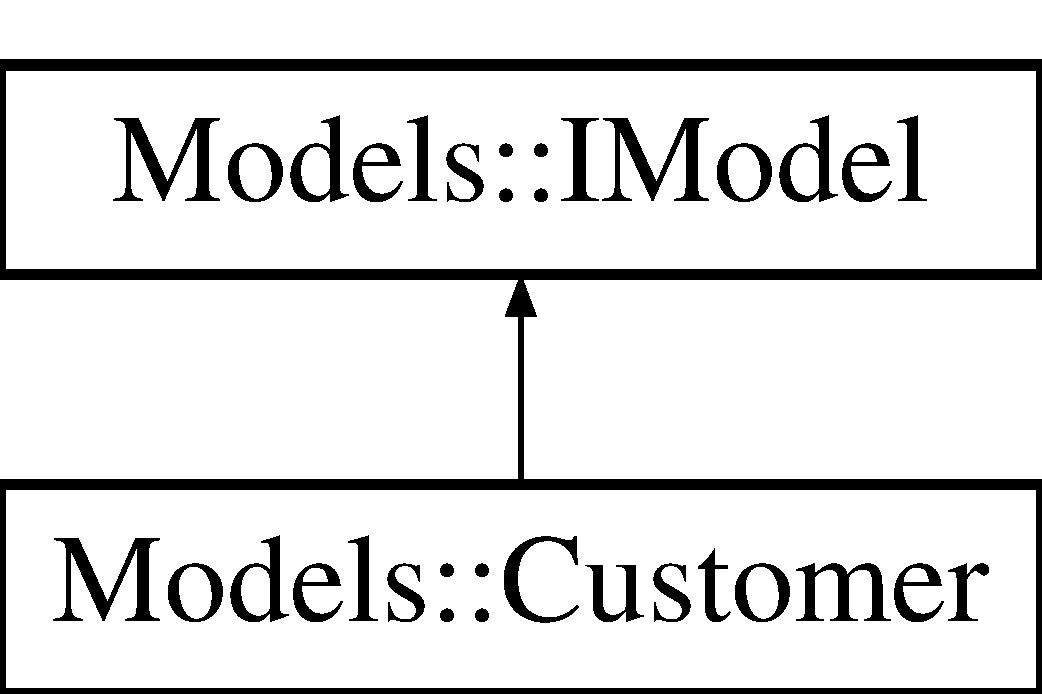
\includegraphics[height=3.000000cm]{db/dd7/classModels_1_1Customer}
\end{center}
\end{figure}
\subsection*{Public Member Functions}
\begin{DoxyCompactItemize}
\item 
\hypertarget{classModels_1_1Customer_a28e8ade7d9ccc39707f823ba8d45f7d0}{\hyperlink{classModels_1_1Customer_a28e8ade7d9ccc39707f823ba8d45f7d0}{Customer} ()}\label{classModels_1_1Customer_a28e8ade7d9ccc39707f823ba8d45f7d0}

\begin{DoxyCompactList}\small\item\em \hyperlink{classModels_1_1Customer_a28e8ade7d9ccc39707f823ba8d45f7d0}{Customer\-::\-Customer} Construct a \hyperlink{classModels_1_1Customer}{Customer}. \end{DoxyCompactList}\item 
\hyperlink{classModels_1_1Customer_a02a1aee507d4ff4f60019070793fe604}{Customer} (int id)
\begin{DoxyCompactList}\small\item\em \hyperlink{classModels_1_1Customer_a28e8ade7d9ccc39707f823ba8d45f7d0}{Customer\-::\-Customer} Constuct a \hyperlink{classModels_1_1Customer}{Customer} who is specidied by {\itshape id} \end{DoxyCompactList}\item 
void \hyperlink{classModels_1_1Customer_af5c0f2b6d80ad9e6bcbfe39b697d65c4}{commit} ()
\begin{DoxyCompactList}\small\item\em \hyperlink{classModels_1_1Customer_a28e8ade7d9ccc39707f823ba8d45f7d0}{Customer\-::\-Customer} Constuct a \hyperlink{classModels_1_1People}{People} who is specidied by {\itshape id} \end{DoxyCompactList}\item 
void \hyperlink{classModels_1_1Customer_afe3ed7fb893d61ea6f4d14e73779382c}{hydrat} (int id)
\begin{DoxyCompactList}\small\item\em \hyperlink{classModels_1_1Customer_afe3ed7fb893d61ea6f4d14e73779382c}{Customer\-::hydrat} Insert into database informations related to the \hyperlink{classModels_1_1Customer}{Customer} who is specified by {\itshape id} \end{DoxyCompactList}\item 
\hypertarget{classModels_1_1Customer_a0f5dba0d90af0adf5d0aca26195d21b1}{void \hyperlink{classModels_1_1Customer_a0f5dba0d90af0adf5d0aca26195d21b1}{remove} ()}\label{classModels_1_1Customer_a0f5dba0d90af0adf5d0aca26195d21b1}

\begin{DoxyCompactList}\small\item\em \hyperlink{classModels_1_1Customer_a0f5dba0d90af0adf5d0aca26195d21b1}{Customer\-::remove} Remove the current customer. \end{DoxyCompactList}\item 
Q\-Variant\-Hash \hyperlink{classModels_1_1Customer_ae72b05319056dc482f3f525ef40b8d40}{get\-Data\-Map} ()
\begin{DoxyCompactList}\small\item\em get\-Data\-Map Get all data of model with a Hash\-Map key/value \end{DoxyCompactList}\item 
Q\-String \hyperlink{classModels_1_1Customer_ac1aec0fb9058333e1a2496b1c29049af}{get\-Path} () const 
\begin{DoxyCompactList}\small\item\em \hyperlink{classModels_1_1Customer_ac1aec0fb9058333e1a2496b1c29049af}{Customer\-::get\-Path} Return the path of the workspace for the current \hyperlink{classModels_1_1Customer}{Customer}. \end{DoxyCompactList}\item 
Q\-String \hyperlink{classModels_1_1Customer_ab7c63946125a6b8d876f0f4e2b50c97e}{get\-Name\-Folder} () const 
\begin{DoxyCompactList}\small\item\em \hyperlink{classModels_1_1Customer_ab7c63946125a6b8d876f0f4e2b50c97e}{Customer\-::get\-Name\-Folder} Return the name of the current \hyperlink{classModels_1_1Customer}{Customer}'s folder in the workspace. \end{DoxyCompactList}\item 
double \hyperlink{classModels_1_1Customer_a193fb1920b53048d8a5f7c8e08581e69}{get\-Turnover} () const 
\begin{DoxyCompactList}\small\item\em \hyperlink{classModels_1_1Customer_a193fb1920b53048d8a5f7c8e08581e69}{Customer\-::get\-Turnover} Return the turnover of the customer money that customer pay, revenue sales. \end{DoxyCompactList}\item 
Q\-Pixmap $\ast$ \hyperlink{classModels_1_1Customer_ab7a4630fa60070dafb42031873c47251}{get\-Image} ()
\begin{DoxyCompactList}\small\item\em \hyperlink{classModels_1_1Customer_ab7a4630fa60070dafb42031873c47251}{Customer\-::get\-Image} Return the compagny image. \end{DoxyCompactList}\item 
void \hyperlink{classModels_1_1Customer_ac164f9bd8221da51ce16a95e9a3890f0}{set\-Image} (Q\-Pixmap $\ast$image)
\begin{DoxyCompactList}\small\item\em \hyperlink{classModels_1_1Customer_ac164f9bd8221da51ce16a95e9a3890f0}{Customer\-::set\-Image} Change the current image by the new {\itshape image} \end{DoxyCompactList}\item 
bool \hyperlink{classModels_1_1Customer_a1dfb958b33d0fcc9892fe902487be43d}{is\-Archived} () const 
\begin{DoxyCompactList}\small\item\em \hyperlink{classModels_1_1Customer_a1dfb958b33d0fcc9892fe902487be43d}{Customer\-::is\-Archived} Return if the {\bfseries \hyperlink{classModels_1_1Customer}{Customer}} is archived. \end{DoxyCompactList}\item 
void \hyperlink{classModels_1_1Customer_a15ec2603da3dd66c9355a9604b5abded}{set\-Is\-Archived} (const bool \hyperlink{classModels_1_1Customer_a1dfb958b33d0fcc9892fe902487be43d}{is\-Archived})
\begin{DoxyCompactList}\small\item\em \hyperlink{classModels_1_1Customer_a15ec2603da3dd66c9355a9604b5abded}{Customer\-::set\-Is\-Archived} set the {\itshape is\-Archived} parameter. \end{DoxyCompactList}\end{DoxyCompactItemize}
\subsection*{Additional Inherited Members}


\subsection{Detailed Description}
The \hyperlink{classModels_1_1Customer}{Customer} class \hyperlink{classModels_1_1Customer}{Customer}. 

\begin{DoxyAuthor}{Author}
Antoine de Roquemaurel 

Florent Berbie 
\end{DoxyAuthor}


\subsection{Constructor \& Destructor Documentation}
\hypertarget{classModels_1_1Customer_a02a1aee507d4ff4f60019070793fe604}{\index{Models\-::\-Customer@{Models\-::\-Customer}!Customer@{Customer}}
\index{Customer@{Customer}!Models::Customer@{Models\-::\-Customer}}
\subsubsection[{Customer}]{\setlength{\rightskip}{0pt plus 5cm}Models\-::\-Customer\-::\-Customer (
\begin{DoxyParamCaption}
\item[{int}]{id}
\end{DoxyParamCaption}
)}}\label{classModels_1_1Customer_a02a1aee507d4ff4f60019070793fe604}


\hyperlink{classModels_1_1Customer_a28e8ade7d9ccc39707f823ba8d45f7d0}{Customer\-::\-Customer} Constuct a \hyperlink{classModels_1_1Customer}{Customer} who is specidied by {\itshape id} 


\begin{DoxyParams}{Parameters}
{\em id} & \hyperlink{classModels_1_1Customer}{Customer} identify \\
\hline
\end{DoxyParams}


\subsection{Member Function Documentation}
\hypertarget{classModels_1_1Customer_af5c0f2b6d80ad9e6bcbfe39b697d65c4}{\index{Models\-::\-Customer@{Models\-::\-Customer}!commit@{commit}}
\index{commit@{commit}!Models::Customer@{Models\-::\-Customer}}
\subsubsection[{commit}]{\setlength{\rightskip}{0pt plus 5cm}void Models\-::\-Customer\-::commit (
\begin{DoxyParamCaption}
{}
\end{DoxyParamCaption}
)\hspace{0.3cm}{\ttfamily [virtual]}}}\label{classModels_1_1Customer_af5c0f2b6d80ad9e6bcbfe39b697d65c4}


\hyperlink{classModels_1_1Customer_a28e8ade7d9ccc39707f823ba8d45f7d0}{Customer\-::\-Customer} Constuct a \hyperlink{classModels_1_1People}{People} who is specidied by {\itshape id} 


\begin{DoxyParams}{Parameters}
{\em id} & \hyperlink{classModels_1_1Customer}{Customer} identify \\
\hline
\end{DoxyParams}


Implements \hyperlink{classModels_1_1IModel_ab4bc529739a8d243222212590888be45}{Models\-::\-I\-Model}.

\hypertarget{classModels_1_1Customer_ae72b05319056dc482f3f525ef40b8d40}{\index{Models\-::\-Customer@{Models\-::\-Customer}!get\-Data\-Map@{get\-Data\-Map}}
\index{get\-Data\-Map@{get\-Data\-Map}!Models::Customer@{Models\-::\-Customer}}
\subsubsection[{get\-Data\-Map}]{\setlength{\rightskip}{0pt plus 5cm}Q\-Variant\-Hash Models\-::\-Customer\-::get\-Data\-Map (
\begin{DoxyParamCaption}
{}
\end{DoxyParamCaption}
)\hspace{0.3cm}{\ttfamily [virtual]}}}\label{classModels_1_1Customer_ae72b05319056dc482f3f525ef40b8d40}


get\-Data\-Map Get all data of model with a Hash\-Map key/value 

\begin{DoxyReturn}{Returns}
Model's data 
\end{DoxyReturn}


Implements \hyperlink{classModels_1_1IModel_a9851b0f296aac58353edff22af11cf3c}{Models\-::\-I\-Model}.

\hypertarget{classModels_1_1Customer_ab7a4630fa60070dafb42031873c47251}{\index{Models\-::\-Customer@{Models\-::\-Customer}!get\-Image@{get\-Image}}
\index{get\-Image@{get\-Image}!Models::Customer@{Models\-::\-Customer}}
\subsubsection[{get\-Image}]{\setlength{\rightskip}{0pt plus 5cm}Q\-Pixmap $\ast$ Models\-::\-Customer\-::get\-Image (
\begin{DoxyParamCaption}
{}
\end{DoxyParamCaption}
)}}\label{classModels_1_1Customer_ab7a4630fa60070dafb42031873c47251}


\hyperlink{classModels_1_1Customer_ab7a4630fa60070dafb42031873c47251}{Customer\-::get\-Image} Return the compagny image. 

\begin{DoxyReturn}{Returns}
compagny image 
\end{DoxyReturn}
\hypertarget{classModels_1_1Customer_ab7c63946125a6b8d876f0f4e2b50c97e}{\index{Models\-::\-Customer@{Models\-::\-Customer}!get\-Name\-Folder@{get\-Name\-Folder}}
\index{get\-Name\-Folder@{get\-Name\-Folder}!Models::Customer@{Models\-::\-Customer}}
\subsubsection[{get\-Name\-Folder}]{\setlength{\rightskip}{0pt plus 5cm}Q\-String Models\-::\-Customer\-::get\-Name\-Folder (
\begin{DoxyParamCaption}
{}
\end{DoxyParamCaption}
) const}}\label{classModels_1_1Customer_ab7c63946125a6b8d876f0f4e2b50c97e}


\hyperlink{classModels_1_1Customer_ab7c63946125a6b8d876f0f4e2b50c97e}{Customer\-::get\-Name\-Folder} Return the name of the current \hyperlink{classModels_1_1Customer}{Customer}'s folder in the workspace. 

\begin{DoxyReturn}{Returns}
name of the \hyperlink{classModels_1_1Customer}{Customer}'s folder 
\end{DoxyReturn}
\hypertarget{classModels_1_1Customer_ac1aec0fb9058333e1a2496b1c29049af}{\index{Models\-::\-Customer@{Models\-::\-Customer}!get\-Path@{get\-Path}}
\index{get\-Path@{get\-Path}!Models::Customer@{Models\-::\-Customer}}
\subsubsection[{get\-Path}]{\setlength{\rightskip}{0pt plus 5cm}Q\-String Models\-::\-Customer\-::get\-Path (
\begin{DoxyParamCaption}
{}
\end{DoxyParamCaption}
) const}}\label{classModels_1_1Customer_ac1aec0fb9058333e1a2496b1c29049af}


\hyperlink{classModels_1_1Customer_ac1aec0fb9058333e1a2496b1c29049af}{Customer\-::get\-Path} Return the path of the workspace for the current \hyperlink{classModels_1_1Customer}{Customer}. 

\begin{DoxyReturn}{Returns}
workspace path 
\end{DoxyReturn}
\hypertarget{classModels_1_1Customer_a193fb1920b53048d8a5f7c8e08581e69}{\index{Models\-::\-Customer@{Models\-::\-Customer}!get\-Turnover@{get\-Turnover}}
\index{get\-Turnover@{get\-Turnover}!Models::Customer@{Models\-::\-Customer}}
\subsubsection[{get\-Turnover}]{\setlength{\rightskip}{0pt plus 5cm}double Models\-::\-Customer\-::get\-Turnover (
\begin{DoxyParamCaption}
{}
\end{DoxyParamCaption}
) const}}\label{classModels_1_1Customer_a193fb1920b53048d8a5f7c8e08581e69}


\hyperlink{classModels_1_1Customer_a193fb1920b53048d8a5f7c8e08581e69}{Customer\-::get\-Turnover} Return the turnover of the customer money that customer pay, revenue sales. 

\begin{DoxyReturn}{Returns}
turnover 
\end{DoxyReturn}
\hypertarget{classModels_1_1Customer_afe3ed7fb893d61ea6f4d14e73779382c}{\index{Models\-::\-Customer@{Models\-::\-Customer}!hydrat@{hydrat}}
\index{hydrat@{hydrat}!Models::Customer@{Models\-::\-Customer}}
\subsubsection[{hydrat}]{\setlength{\rightskip}{0pt plus 5cm}void Models\-::\-Customer\-::hydrat (
\begin{DoxyParamCaption}
\item[{int}]{id}
\end{DoxyParamCaption}
)\hspace{0.3cm}{\ttfamily [virtual]}}}\label{classModels_1_1Customer_afe3ed7fb893d61ea6f4d14e73779382c}


\hyperlink{classModels_1_1Customer_afe3ed7fb893d61ea6f4d14e73779382c}{Customer\-::hydrat} Insert into database informations related to the \hyperlink{classModels_1_1Customer}{Customer} who is specified by {\itshape id} 


\begin{DoxyParams}{Parameters}
{\em id} & \hyperlink{classModels_1_1Customer}{Customer} identify \\
\hline
\end{DoxyParams}


Implements \hyperlink{classModels_1_1IModel_a7ce6def437f5e1f6a78ee1d67ca028e4}{Models\-::\-I\-Model}.

\hypertarget{classModels_1_1Customer_a1dfb958b33d0fcc9892fe902487be43d}{\index{Models\-::\-Customer@{Models\-::\-Customer}!is\-Archived@{is\-Archived}}
\index{is\-Archived@{is\-Archived}!Models::Customer@{Models\-::\-Customer}}
\subsubsection[{is\-Archived}]{\setlength{\rightskip}{0pt plus 5cm}bool Models\-::\-Customer\-::is\-Archived (
\begin{DoxyParamCaption}
{}
\end{DoxyParamCaption}
) const}}\label{classModels_1_1Customer_a1dfb958b33d0fcc9892fe902487be43d}


\hyperlink{classModels_1_1Customer_a1dfb958b33d0fcc9892fe902487be43d}{Customer\-::is\-Archived} Return if the {\bfseries \hyperlink{classModels_1_1Customer}{Customer}} is archived. 

\begin{DoxyReturn}{Returns}
true or false 
\end{DoxyReturn}
\hypertarget{classModels_1_1Customer_ac164f9bd8221da51ce16a95e9a3890f0}{\index{Models\-::\-Customer@{Models\-::\-Customer}!set\-Image@{set\-Image}}
\index{set\-Image@{set\-Image}!Models::Customer@{Models\-::\-Customer}}
\subsubsection[{set\-Image}]{\setlength{\rightskip}{0pt plus 5cm}void Models\-::\-Customer\-::set\-Image (
\begin{DoxyParamCaption}
\item[{Q\-Pixmap $\ast$}]{image}
\end{DoxyParamCaption}
)\hspace{0.3cm}{\ttfamily [virtual]}}}\label{classModels_1_1Customer_ac164f9bd8221da51ce16a95e9a3890f0}


\hyperlink{classModels_1_1Customer_ac164f9bd8221da51ce16a95e9a3890f0}{Customer\-::set\-Image} Change the current image by the new {\itshape image} 


\begin{DoxyParams}{Parameters}
{\em image} & New image \\
\hline
\end{DoxyParams}


Reimplemented from \hyperlink{classModels_1_1People_a020ff3cb4cd47b7a34359fb681afe530}{Models\-::\-People}.

\hypertarget{classModels_1_1Customer_a15ec2603da3dd66c9355a9604b5abded}{\index{Models\-::\-Customer@{Models\-::\-Customer}!set\-Is\-Archived@{set\-Is\-Archived}}
\index{set\-Is\-Archived@{set\-Is\-Archived}!Models::Customer@{Models\-::\-Customer}}
\subsubsection[{set\-Is\-Archived}]{\setlength{\rightskip}{0pt plus 5cm}void Models\-::\-Customer\-::set\-Is\-Archived (
\begin{DoxyParamCaption}
\item[{const bool}]{is\-Archived}
\end{DoxyParamCaption}
)}}\label{classModels_1_1Customer_a15ec2603da3dd66c9355a9604b5abded}


\hyperlink{classModels_1_1Customer_a15ec2603da3dd66c9355a9604b5abded}{Customer\-::set\-Is\-Archived} set the {\itshape is\-Archived} parameter. 


\begin{DoxyParams}{Parameters}
{\em is\-Archived} & \\
\hline
\end{DoxyParams}


The documentation for this class was generated from the following files\-:\begin{DoxyCompactItemize}
\item 
/home/travis/build/\-F\-A\-C\-T-\/\-Team/\-Fact\-Dev/src/models/customer.\-h\item 
/home/travis/build/\-F\-A\-C\-T-\/\-Team/\-Fact\-Dev/src/models/customer.\-cpp\end{DoxyCompactItemize}

\hypertarget{classGui_1_1Widgets_1_1CustomerContextualMenu}{}\section{Gui\+:\+:Widgets\+:\+:Customer\+Contextual\+Menu Class Reference}
\label{classGui_1_1Widgets_1_1CustomerContextualMenu}\index{Gui\+::\+Widgets\+::\+Customer\+Contextual\+Menu@{Gui\+::\+Widgets\+::\+Customer\+Contextual\+Menu}}


Display contextual menu on a customer.  




{\ttfamily \#include $<$customercontextualmenu.\+h$>$}

Inheritance diagram for Gui\+:\+:Widgets\+:\+:Customer\+Contextual\+Menu\+:\begin{figure}[H]
\begin{center}
\leavevmode
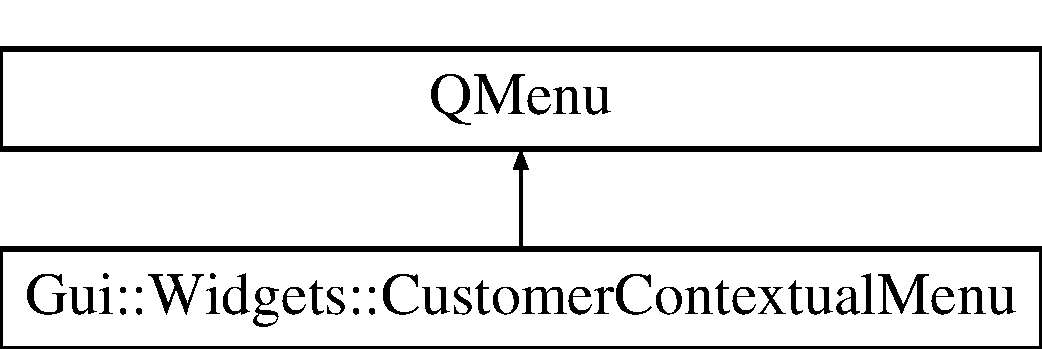
\includegraphics[height=2.000000cm]{d8/ded/classGui_1_1Widgets_1_1CustomerContextualMenu}
\end{center}
\end{figure}
\subsection*{Public Member Functions}
\begin{DoxyCompactItemize}
\item 
\hyperlink{classGui_1_1Widgets_1_1CustomerContextualMenu_ab8fc199bd6adf21f7dd5e881e0a73b16}{Customer\+Contextual\+Menu} (Q\+Widget $\ast$w=0)
\begin{DoxyCompactList}\small\item\em \hyperlink{classGui_1_1Widgets_1_1CustomerContextualMenu_ab8fc199bd6adf21f7dd5e881e0a73b16}{Customer\+Contextual\+Menu\+::\+Customer\+Contextual\+Menu} Construct a new contextual menu. \end{DoxyCompactList}\item 
\hypertarget{classGui_1_1Widgets_1_1CustomerContextualMenu_a6814dcf744752f9026c85a9640cf23ef}{}\hyperlink{classGui_1_1Widgets_1_1CustomerContextualMenu_a6814dcf744752f9026c85a9640cf23ef}{$\sim$\+Customer\+Contextual\+Menu} ()\label{classGui_1_1Widgets_1_1CustomerContextualMenu_a6814dcf744752f9026c85a9640cf23ef}

\begin{DoxyCompactList}\small\item\em Customer\+Contextual\+Menu\+::\+Destruct the contextual menu. \end{DoxyCompactList}\end{DoxyCompactItemize}


\subsection{Detailed Description}
Display contextual menu on a customer. 

\begin{DoxyAuthor}{Author}
Antoine de Roquemaurel 
\end{DoxyAuthor}


\subsection{Constructor \& Destructor Documentation}
\hypertarget{classGui_1_1Widgets_1_1CustomerContextualMenu_ab8fc199bd6adf21f7dd5e881e0a73b16}{}\index{Gui\+::\+Widgets\+::\+Customer\+Contextual\+Menu@{Gui\+::\+Widgets\+::\+Customer\+Contextual\+Menu}!Customer\+Contextual\+Menu@{Customer\+Contextual\+Menu}}
\index{Customer\+Contextual\+Menu@{Customer\+Contextual\+Menu}!Gui\+::\+Widgets\+::\+Customer\+Contextual\+Menu@{Gui\+::\+Widgets\+::\+Customer\+Contextual\+Menu}}
\subsubsection[{Customer\+Contextual\+Menu}]{\setlength{\rightskip}{0pt plus 5cm}Gui\+::\+Widgets\+::\+Customer\+Contextual\+Menu\+::\+Customer\+Contextual\+Menu (
\begin{DoxyParamCaption}
\item[{Q\+Widget $\ast$}]{w = {\ttfamily 0}}
\end{DoxyParamCaption}
)}\label{classGui_1_1Widgets_1_1CustomerContextualMenu_ab8fc199bd6adf21f7dd5e881e0a73b16}


\hyperlink{classGui_1_1Widgets_1_1CustomerContextualMenu_ab8fc199bd6adf21f7dd5e881e0a73b16}{Customer\+Contextual\+Menu\+::\+Customer\+Contextual\+Menu} Construct a new contextual menu. 


\begin{DoxyParams}{Parameters}
{\em w} & Parent \\
\hline
\end{DoxyParams}


The documentation for this class was generated from the following files\+:\begin{DoxyCompactItemize}
\item 
src/gui/widgets/customercontextualmenu.\+h\item 
src/gui/widgets/customercontextualmenu.\+cpp\end{DoxyCompactItemize}

\hypertarget{classDatabase_1_1CustomerDatabase}{\section{Database\+:\+:Customer\+Database Class Reference}
\label{classDatabase_1_1CustomerDatabase}\index{Database\+::\+Customer\+Database@{Database\+::\+Customer\+Database}}
}


The {\bfseries \hyperlink{classDatabase_1_1CustomerDatabase}{Customer\+Database}} class Customer table database.  




{\ttfamily \#include $<$customerdatabase.\+h$>$}

Inheritance diagram for Database\+:\+:Customer\+Database\+:\begin{figure}[H]
\begin{center}
\leavevmode
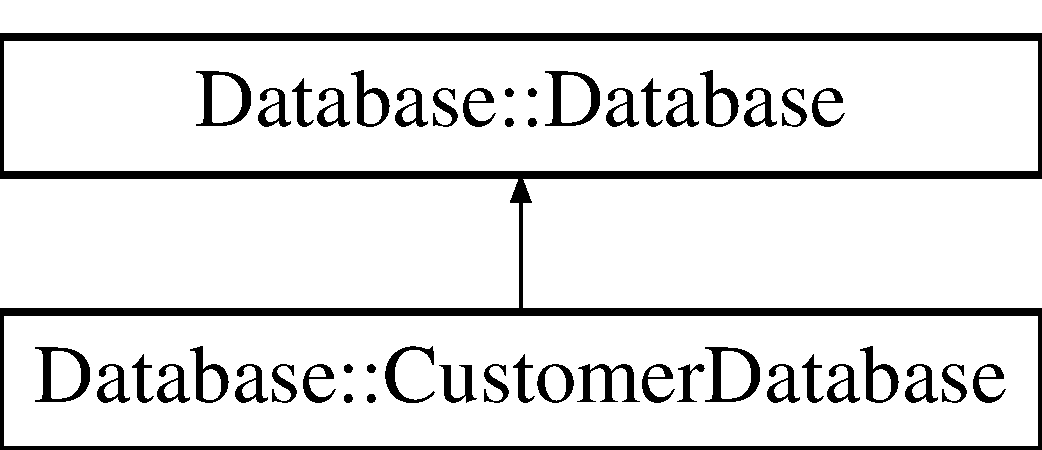
\includegraphics[height=2.000000cm]{de/de4/classDatabase_1_1CustomerDatabase}
\end{center}
\end{figure}
\subsection*{Public Member Functions}
\begin{DoxyCompactItemize}
\item 
Q\+Standard\+Item\+Model $\ast$ \hyperlink{classDatabase_1_1CustomerDatabase_a03110432af547dbe5447c51392cae53a}{get\+Customers\+Table} (Q\+String filter=\char`\"{}\char`\"{})  throw (\+Db\+Exception$\ast$)
\begin{DoxyCompactList}\small\item\em \hyperlink{classDatabase_1_1CustomerDatabase_a03110432af547dbe5447c51392cae53a}{Customer\+Database\+::get\+Customers\+Table} Return an item model of customers for Q\+Table\+View. \end{DoxyCompactList}\item 
Q\+Standard\+Item\+Model $\ast$ \hyperlink{classDatabase_1_1CustomerDatabase_a158c95d767ccf6f4345dd54854088e4f}{get\+Customers\+Tree} (Q\+String filter=\char`\"{}\char`\"{})  throw (\+Db\+Exception$\ast$)
\begin{DoxyCompactList}\small\item\em \hyperlink{classDatabase_1_1CustomerDatabase_a158c95d767ccf6f4345dd54854088e4f}{Customer\+Database\+::get\+Customers\+Tree} Return an item model of customers for Q\+Tree. \end{DoxyCompactList}\item 
Q\+Shared\+Pointer$<$ \hyperlink{classModels_1_1Customer}{Models\+::\+Customer} $>$ \hyperlink{classDatabase_1_1CustomerDatabase_a997eac5e1a9e4d27a4380d10e8f8d935}{get\+Customer} (const int p\+Id)
\begin{DoxyCompactList}\small\item\em \hyperlink{classDatabase_1_1CustomerDatabase_a997eac5e1a9e4d27a4380d10e8f8d935}{Customer\+Database\+::get\+Customer} get informations about the customer identified by {\itshape p\+Id} \end{DoxyCompactList}\item 
int \hyperlink{classDatabase_1_1CustomerDatabase_a10331f3013c56e9d9140d9c2e6d64b30}{add\+Customer} (const \hyperlink{classModels_1_1Customer}{Models\+::\+Customer} \&)
\begin{DoxyCompactList}\small\item\em \hyperlink{classDatabase_1_1CustomerDatabase_a10331f3013c56e9d9140d9c2e6d64b30}{Customer\+Database\+::add\+Customer} Add the customer {\itshape p\+Customer} to the database. \end{DoxyCompactList}\item 
\hypertarget{classDatabase_1_1CustomerDatabase_a8408b97565455420fe062b5d62c19088}{void \hyperlink{classDatabase_1_1CustomerDatabase_a8408b97565455420fe062b5d62c19088}{update\+Customer} (const \hyperlink{classModels_1_1Customer}{Models\+::\+Customer} \&)}\label{classDatabase_1_1CustomerDatabase_a8408b97565455420fe062b5d62c19088}

\begin{DoxyCompactList}\small\item\em \hyperlink{classDatabase_1_1CustomerDatabase_a8408b97565455420fe062b5d62c19088}{Customer\+Database\+::update\+Customer} Update informations about the customer {\itshape p\+Customer} \end{DoxyCompactList}\item 
void \hyperlink{classDatabase_1_1CustomerDatabase_ad19fe8efe5e718aba97c9b1a606553c7}{remove\+Customer} (const int p\+Id)
\begin{DoxyCompactList}\small\item\em \hyperlink{classDatabase_1_1CustomerDatabase_ad19fe8efe5e718aba97c9b1a606553c7}{Customer\+Database\+::remove\+Customer} Remove the customer with the id {\itshape p\+Id} \end{DoxyCompactList}\item 
int \hyperlink{classDatabase_1_1CustomerDatabase_a73d49c62c59c63607d3b1bf9c03328cb}{get\+Nb\+Customers} ()
\begin{DoxyCompactList}\small\item\em \hyperlink{classDatabase_1_1CustomerDatabase_a73d49c62c59c63607d3b1bf9c03328cb}{Customer\+Database\+::get\+Nb\+Customers} Return the number of customers existing. \end{DoxyCompactList}\end{DoxyCompactItemize}
\subsection*{Static Public Member Functions}
\begin{DoxyCompactItemize}
\item 
static \hyperlink{classDatabase_1_1CustomerDatabase}{Customer\+Database} $\ast$ \hyperlink{classDatabase_1_1CustomerDatabase_adfa3f1c75bedb1b0112c06ddc1418f77}{instance} ()  throw (\+Db\+Exception$\ast$)
\begin{DoxyCompactList}\small\item\em Customer\+Database\+::get\+Instance Return an instance of {\bfseries \hyperlink{classDatabase_1_1CustomerDatabase}{Customer\+Database}} \end{DoxyCompactList}\end{DoxyCompactItemize}
\subsection*{Additional Inherited Members}


\subsection{Detailed Description}
The {\bfseries \hyperlink{classDatabase_1_1CustomerDatabase}{Customer\+Database}} class Customer table database. 

\begin{DoxyAuthor}{Author}
Antoine de Roquemaurel 
\end{DoxyAuthor}
\begin{DoxySeeAlso}{See also}
\hyperlink{classDatabase_1_1Database}{Database} 

Customer 
\end{DoxySeeAlso}


\subsection{Member Function Documentation}
\hypertarget{classDatabase_1_1CustomerDatabase_a10331f3013c56e9d9140d9c2e6d64b30}{\index{Database\+::\+Customer\+Database@{Database\+::\+Customer\+Database}!add\+Customer@{add\+Customer}}
\index{add\+Customer@{add\+Customer}!Database\+::\+Customer\+Database@{Database\+::\+Customer\+Database}}
\subsubsection[{add\+Customer}]{\setlength{\rightskip}{0pt plus 5cm}int Database\+::\+Customer\+Database\+::add\+Customer (
\begin{DoxyParamCaption}
\item[{const {\bf Models\+::\+Customer} \&}]{p\+Customer}
\end{DoxyParamCaption}
)}}\label{classDatabase_1_1CustomerDatabase_a10331f3013c56e9d9140d9c2e6d64b30}


\hyperlink{classDatabase_1_1CustomerDatabase_a10331f3013c56e9d9140d9c2e6d64b30}{Customer\+Database\+::add\+Customer} Add the customer {\itshape p\+Customer} to the database. 

\begin{DoxyReturn}{Returns}
customer id 
\end{DoxyReturn}
\hypertarget{classDatabase_1_1CustomerDatabase_a997eac5e1a9e4d27a4380d10e8f8d935}{\index{Database\+::\+Customer\+Database@{Database\+::\+Customer\+Database}!get\+Customer@{get\+Customer}}
\index{get\+Customer@{get\+Customer}!Database\+::\+Customer\+Database@{Database\+::\+Customer\+Database}}
\subsubsection[{get\+Customer}]{\setlength{\rightskip}{0pt plus 5cm}Q\+Shared\+Pointer$<$ {\bf Models\+::\+Customer} $>$ Database\+::\+Customer\+Database\+::get\+Customer (
\begin{DoxyParamCaption}
\item[{const int}]{p\+Id}
\end{DoxyParamCaption}
)}}\label{classDatabase_1_1CustomerDatabase_a997eac5e1a9e4d27a4380d10e8f8d935}


\hyperlink{classDatabase_1_1CustomerDatabase_a997eac5e1a9e4d27a4380d10e8f8d935}{Customer\+Database\+::get\+Customer} get informations about the customer identified by {\itshape p\+Id} 


\begin{DoxyParams}{Parameters}
{\em p\+Id} & customer id \\
\hline
\end{DoxyParams}
\begin{DoxyReturn}{Returns}
the Customer 
\end{DoxyReturn}
\hypertarget{classDatabase_1_1CustomerDatabase_a03110432af547dbe5447c51392cae53a}{\index{Database\+::\+Customer\+Database@{Database\+::\+Customer\+Database}!get\+Customers\+Table@{get\+Customers\+Table}}
\index{get\+Customers\+Table@{get\+Customers\+Table}!Database\+::\+Customer\+Database@{Database\+::\+Customer\+Database}}
\subsubsection[{get\+Customers\+Table}]{\setlength{\rightskip}{0pt plus 5cm}Q\+Standard\+Item\+Model $\ast$ Database\+::\+Customer\+Database\+::get\+Customers\+Table (
\begin{DoxyParamCaption}
\item[{Q\+String}]{filter = {\ttfamily \char`\"{}\char`\"{}}}
\end{DoxyParamCaption}
) throw  {\bf Db\+Exception} $\ast$) }}\label{classDatabase_1_1CustomerDatabase_a03110432af547dbe5447c51392cae53a}


\hyperlink{classDatabase_1_1CustomerDatabase_a03110432af547dbe5447c51392cae53a}{Customer\+Database\+::get\+Customers\+Table} Return an item model of customers for Q\+Table\+View. 

\begin{DoxyAuthor}{Author}
Manantsoa Razanajatovo 
\end{DoxyAuthor}

\begin{DoxyParams}{Parameters}
{\em filter} & Select only customers who are specified by {\itshape filter} \\
\hline
\end{DoxyParams}

\begin{DoxyExceptions}{Exceptions}
{\em Db\+Exception} & \\
\hline
\end{DoxyExceptions}
\begin{DoxyReturn}{Returns}
Q\+Standard\+Item\+Model an item model for Q\+Table\+View 
\end{DoxyReturn}
\hypertarget{classDatabase_1_1CustomerDatabase_a158c95d767ccf6f4345dd54854088e4f}{\index{Database\+::\+Customer\+Database@{Database\+::\+Customer\+Database}!get\+Customers\+Tree@{get\+Customers\+Tree}}
\index{get\+Customers\+Tree@{get\+Customers\+Tree}!Database\+::\+Customer\+Database@{Database\+::\+Customer\+Database}}
\subsubsection[{get\+Customers\+Tree}]{\setlength{\rightskip}{0pt plus 5cm}Q\+Standard\+Item\+Model $\ast$ Database\+::\+Customer\+Database\+::get\+Customers\+Tree (
\begin{DoxyParamCaption}
\item[{Q\+String}]{filter = {\ttfamily \char`\"{}\char`\"{}}}
\end{DoxyParamCaption}
) throw  {\bf Db\+Exception} $\ast$) }}\label{classDatabase_1_1CustomerDatabase_a158c95d767ccf6f4345dd54854088e4f}


\hyperlink{classDatabase_1_1CustomerDatabase_a158c95d767ccf6f4345dd54854088e4f}{Customer\+Database\+::get\+Customers\+Tree} Return an item model of customers for Q\+Tree. 

\begin{DoxyAuthor}{Author}
Manantsoa Razanajatovo 
\end{DoxyAuthor}

\begin{DoxyParams}{Parameters}
{\em filter} & Select only customers who are specified by {\itshape filter} \\
\hline
\end{DoxyParams}

\begin{DoxyExceptions}{Exceptions}
{\em Db\+Exception} & \\
\hline
\end{DoxyExceptions}
\begin{DoxyReturn}{Returns}
Q\+Standard\+Item\+Model an item model for Q\+Tree\+View 
\end{DoxyReturn}
\hypertarget{classDatabase_1_1CustomerDatabase_a73d49c62c59c63607d3b1bf9c03328cb}{\index{Database\+::\+Customer\+Database@{Database\+::\+Customer\+Database}!get\+Nb\+Customers@{get\+Nb\+Customers}}
\index{get\+Nb\+Customers@{get\+Nb\+Customers}!Database\+::\+Customer\+Database@{Database\+::\+Customer\+Database}}
\subsubsection[{get\+Nb\+Customers}]{\setlength{\rightskip}{0pt plus 5cm}int Database\+::\+Customer\+Database\+::get\+Nb\+Customers (
\begin{DoxyParamCaption}
{}
\end{DoxyParamCaption}
)}}\label{classDatabase_1_1CustomerDatabase_a73d49c62c59c63607d3b1bf9c03328cb}


\hyperlink{classDatabase_1_1CustomerDatabase_a73d49c62c59c63607d3b1bf9c03328cb}{Customer\+Database\+::get\+Nb\+Customers} Return the number of customers existing. 

\begin{DoxyReturn}{Returns}
number of customers 
\end{DoxyReturn}
\hypertarget{classDatabase_1_1CustomerDatabase_adfa3f1c75bedb1b0112c06ddc1418f77}{\index{Database\+::\+Customer\+Database@{Database\+::\+Customer\+Database}!instance@{instance}}
\index{instance@{instance}!Database\+::\+Customer\+Database@{Database\+::\+Customer\+Database}}
\subsubsection[{instance}]{\setlength{\rightskip}{0pt plus 5cm}{\bf Customer\+Database} $\ast$ Database\+::\+Customer\+Database\+::instance (
\begin{DoxyParamCaption}
{}
\end{DoxyParamCaption}
) throw  {\bf Db\+Exception} $\ast$) \hspace{0.3cm}{\ttfamily [static]}}}\label{classDatabase_1_1CustomerDatabase_adfa3f1c75bedb1b0112c06ddc1418f77}


Customer\+Database\+::get\+Instance Return an instance of {\bfseries \hyperlink{classDatabase_1_1CustomerDatabase}{Customer\+Database}} 

\begin{DoxySeeAlso}{See also}
Db\+Exception 
\end{DoxySeeAlso}
\begin{DoxyReturn}{Returns}
Instance of \hyperlink{classDatabase_1_1CustomerDatabase}{Customer\+Database} 
\end{DoxyReturn}
\hypertarget{classDatabase_1_1CustomerDatabase_ad19fe8efe5e718aba97c9b1a606553c7}{\index{Database\+::\+Customer\+Database@{Database\+::\+Customer\+Database}!remove\+Customer@{remove\+Customer}}
\index{remove\+Customer@{remove\+Customer}!Database\+::\+Customer\+Database@{Database\+::\+Customer\+Database}}
\subsubsection[{remove\+Customer}]{\setlength{\rightskip}{0pt plus 5cm}void Database\+::\+Customer\+Database\+::remove\+Customer (
\begin{DoxyParamCaption}
\item[{const int}]{p\+Id}
\end{DoxyParamCaption}
)}}\label{classDatabase_1_1CustomerDatabase_ad19fe8efe5e718aba97c9b1a606553c7}


\hyperlink{classDatabase_1_1CustomerDatabase_ad19fe8efe5e718aba97c9b1a606553c7}{Customer\+Database\+::remove\+Customer} Remove the customer with the id {\itshape p\+Id} 


\begin{DoxyParams}{Parameters}
{\em p\+Id} & customer id \\
\hline
\end{DoxyParams}


The documentation for this class was generated from the following files\+:\begin{DoxyCompactItemize}
\item 
src/database/customerdatabase.\+h\item 
src/database/customerdatabase.\+cpp\end{DoxyCompactItemize}

\hypertarget{classCustomerDatabaseTest}{\section{Customer\-Database\-Test Class Reference}
\label{classCustomerDatabaseTest}\index{Customer\-Database\-Test@{Customer\-Database\-Test}}
}
Inheritance diagram for Customer\-Database\-Test\-:\begin{figure}[H]
\begin{center}
\leavevmode
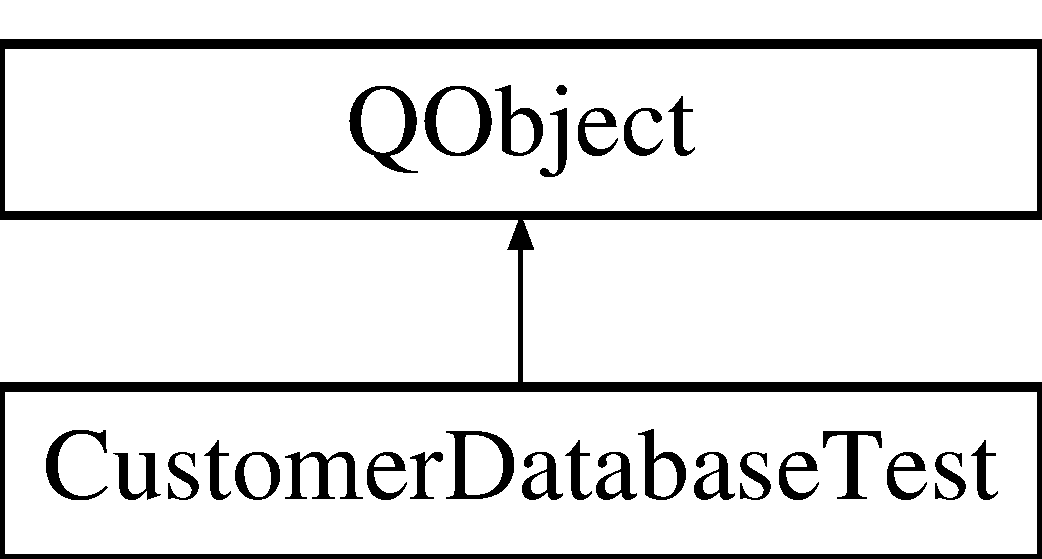
\includegraphics[height=2.000000cm]{d2/d63/classCustomerDatabaseTest}
\end{center}
\end{figure}


The documentation for this class was generated from the following files\-:\begin{DoxyCompactItemize}
\item 
/home/florent/\-Documents/\-Projet\-\_\-\-S8/\-Fact\-Dev/tests/database/customerdatabasetest.\-h\item 
/home/florent/\-Documents/\-Projet\-\_\-\-S8/\-Fact\-Dev/tests/database/customerdatabasetest.\-cpp\end{DoxyCompactItemize}

\hypertarget{classGui_1_1Widgets_1_1CustomerDataWidget}{\section{Gui\-:\-:Widgets\-:\-:Customer\-Data\-Widget Class Reference}
\label{classGui_1_1Widgets_1_1CustomerDataWidget}\index{Gui\-::\-Widgets\-::\-Customer\-Data\-Widget@{Gui\-::\-Widgets\-::\-Customer\-Data\-Widget}}
}


Class for display info of a customer.  




{\ttfamily \#include $<$customerdatawidget.\-h$>$}

Inheritance diagram for Gui\-:\-:Widgets\-:\-:Customer\-Data\-Widget\-:\begin{figure}[H]
\begin{center}
\leavevmode
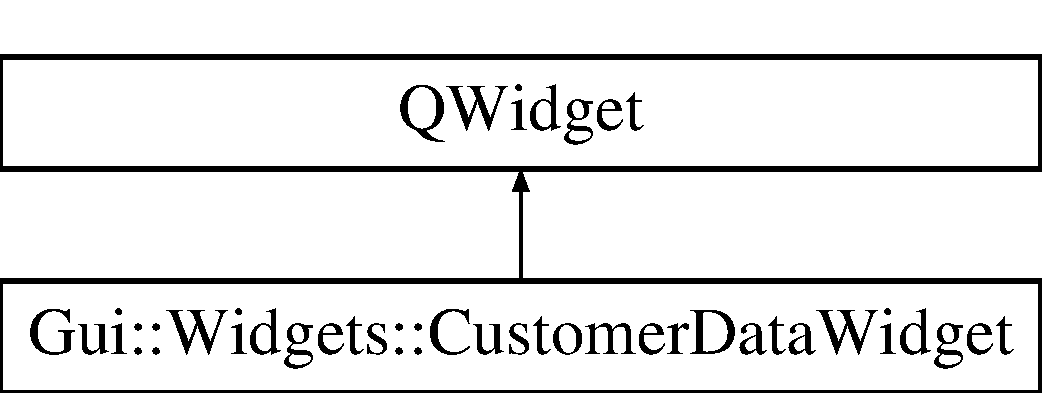
\includegraphics[height=2.000000cm]{df/deb/classGui_1_1Widgets_1_1CustomerDataWidget}
\end{center}
\end{figure}
\subsection*{Public Member Functions}
\begin{DoxyCompactItemize}
\item 
\hypertarget{classGui_1_1Widgets_1_1CustomerDataWidget_a649d25216952fa8642b22983a07c9186}{{\bfseries Customer\-Data\-Widget} (Q\-Widget $\ast$parent=0)}\label{classGui_1_1Widgets_1_1CustomerDataWidget_a649d25216952fa8642b22983a07c9186}

\item 
\hypertarget{classGui_1_1Widgets_1_1CustomerDataWidget_a78504b749fc7d80302c27748a4033b1f}{void \hyperlink{classGui_1_1Widgets_1_1CustomerDataWidget_a78504b749fc7d80302c27748a4033b1f}{print\-User\-Data} ()}\label{classGui_1_1Widgets_1_1CustomerDataWidget_a78504b749fc7d80302c27748a4033b1f}

\begin{DoxyCompactList}\small\item\em print\-User\-Data Print Data of current user \end{DoxyCompactList}\item 
void \hyperlink{classGui_1_1Widgets_1_1CustomerDataWidget_aa995ed95c5ca119db4258af2fe403691}{print\-Informations} (int id)
\begin{DoxyCompactList}\small\item\em print\-Informations Print Data of customer id \end{DoxyCompactList}\end{DoxyCompactItemize}


\subsection{Detailed Description}
Class for display info of a customer. 

\begin{DoxyAuthor}{Author}

\end{DoxyAuthor}


\subsection{Member Function Documentation}
\hypertarget{classGui_1_1Widgets_1_1CustomerDataWidget_aa995ed95c5ca119db4258af2fe403691}{\index{Gui\-::\-Widgets\-::\-Customer\-Data\-Widget@{Gui\-::\-Widgets\-::\-Customer\-Data\-Widget}!print\-Informations@{print\-Informations}}
\index{print\-Informations@{print\-Informations}!Gui::Widgets::CustomerDataWidget@{Gui\-::\-Widgets\-::\-Customer\-Data\-Widget}}
\subsubsection[{print\-Informations}]{\setlength{\rightskip}{0pt plus 5cm}void Gui\-::\-Widgets\-::\-Customer\-Data\-Widget\-::print\-Informations (
\begin{DoxyParamCaption}
\item[{int}]{id}
\end{DoxyParamCaption}
)}}\label{classGui_1_1Widgets_1_1CustomerDataWidget_aa995ed95c5ca119db4258af2fe403691}


print\-Informations Print Data of customer id 


\begin{DoxyParams}{Parameters}
{\em id} & of customer to print \\
\hline
\end{DoxyParams}


The documentation for this class was generated from the following files\-:\begin{DoxyCompactItemize}
\item 
/home/travis/build/\-F\-A\-C\-T-\/\-Team/\-Fact\-Dev/src/gui/widgets/customerdatawidget.\-h\item 
/home/travis/build/\-F\-A\-C\-T-\/\-Team/\-Fact\-Dev/src/gui/widgets/customerdatawidget.\-cpp\end{DoxyCompactItemize}

\hypertarget{classCustomerModelTest}{\section{Customer\-Model\-Test Class Reference}
\label{classCustomerModelTest}\index{Customer\-Model\-Test@{Customer\-Model\-Test}}
}
Inheritance diagram for Customer\-Model\-Test\-:\begin{figure}[H]
\begin{center}
\leavevmode
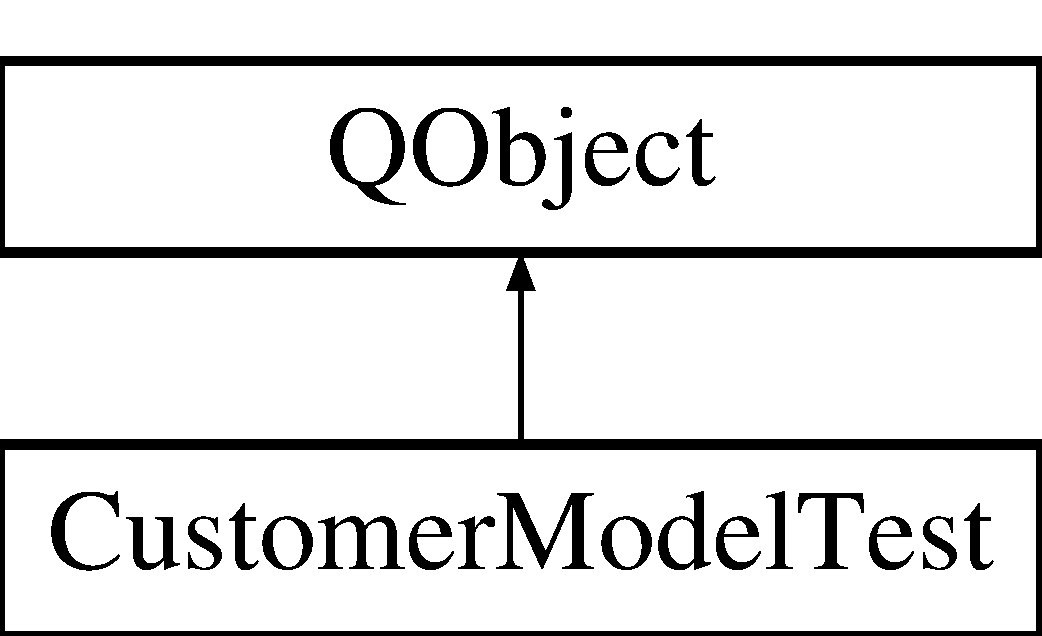
\includegraphics[height=2.000000cm]{d5/dcd/classCustomerModelTest}
\end{center}
\end{figure}


The documentation for this class was generated from the following files\-:\begin{DoxyCompactItemize}
\item 
/home/travis/build/\-F\-A\-C\-T-\/\-Team/\-Fact\-Dev/tests/models/customermodeltest.\-h\item 
/home/travis/build/\-F\-A\-C\-T-\/\-Team/\-Fact\-Dev/tests/models/customermodeltest.\-cpp\end{DoxyCompactItemize}

\hypertarget{classDatabase_1_1Database}{\section{Database\+:\+:Database Class Reference}
\label{classDatabase_1_1Database}\index{Database\+::\+Database@{Database\+::\+Database}}
}


The {\bfseries \hyperlink{classDatabase_1_1Database}{Database}} class Master class for all database access.  




{\ttfamily \#include $<$database.\+h$>$}

Inheritance diagram for Database\+:\+:Database\+:\begin{figure}[H]
\begin{center}
\leavevmode
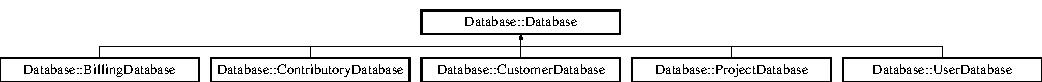
\includegraphics[height=1.108911cm]{da/d8e/classDatabase_1_1Database}
\end{center}
\end{figure}
\subsection*{Public Member Functions}
\begin{DoxyCompactItemize}
\item 
Q\+String \hyperlink{classDatabase_1_1Database_aff2b9057350d618d9f126a0e6ac6be42}{last\+Error} (const Q\+Sql\+Query \&q)
\begin{DoxyCompactList}\small\item\em Database\+::last\+Error Return an error message on the last error occured during the S\+Q\+L request {\itshape q} \end{DoxyCompactList}\item 
\hypertarget{classDatabase_1_1Database_a77460984575eb485e3c6dcfc713e0e67}{void \hyperlink{classDatabase_1_1Database_a77460984575eb485e3c6dcfc713e0e67}{test\+Cases} ()}\label{classDatabase_1_1Database_a77460984575eb485e3c6dcfc713e0e67}

\begin{DoxyCompactList}\small\item\em Database\+::test\+Cases Realise a test cases. \end{DoxyCompactList}\item 
\hypertarget{classDatabase_1_1Database_a474fda5b2ee6cd1391f72ad5fe297ba5}{void \hyperlink{classDatabase_1_1Database_a474fda5b2ee6cd1391f72ad5fe297ba5}{clean\+Database} ()}\label{classDatabase_1_1Database_a474fda5b2ee6cd1391f72ad5fe297ba5}

\begin{DoxyCompactList}\small\item\em Database\+::vider\+Database Clear database. \end{DoxyCompactList}\item 
void \hyperlink{classDatabase_1_1Database_a8fa0ebf8b613b8c25f2485dee5c332f3}{execute\+File} (Q\+String p\+Name)
\begin{DoxyCompactList}\small\item\em Database\+::executer\+Fichier Exeute a specified file named {\itshape p\+Name} \end{DoxyCompactList}\item 
\hypertarget{classDatabase_1_1Database_a657a65d7c085ef1b3fbc956d5c837ec0}{void \hyperlink{classDatabase_1_1Database_a657a65d7c085ef1b3fbc956d5c837ec0}{open\+Transaction} ()}\label{classDatabase_1_1Database_a657a65d7c085ef1b3fbc956d5c837ec0}

\begin{DoxyCompactList}\small\item\em Database\+::open\+Transaction Open new transaction. \end{DoxyCompactList}\item 
\hypertarget{classDatabase_1_1Database_a7cb02c000e1bc3614aeda31ea6c13069}{void \hyperlink{classDatabase_1_1Database_a7cb02c000e1bc3614aeda31ea6c13069}{close\+Transaction} ()}\label{classDatabase_1_1Database_a7cb02c000e1bc3614aeda31ea6c13069}

\begin{DoxyCompactList}\small\item\em Database\+::close\+Transaction Close current transaction. \end{DoxyCompactList}\item 
\hypertarget{classDatabase_1_1Database_af4d88f98b0ce31369af5bbf4fd167664}{void \hyperlink{classDatabase_1_1Database_af4d88f98b0ce31369af5bbf4fd167664}{close} ()}\label{classDatabase_1_1Database_af4d88f98b0ce31369af5bbf4fd167664}

\begin{DoxyCompactList}\small\item\em Database\+::close Close database access. \end{DoxyCompactList}\item 
\hypertarget{classDatabase_1_1Database_aa12f5d991eb4d61ef0c6a0bc653f2580}{void \hyperlink{classDatabase_1_1Database_aa12f5d991eb4d61ef0c6a0bc653f2580}{open} ()}\label{classDatabase_1_1Database_aa12f5d991eb4d61ef0c6a0bc653f2580}

\begin{DoxyCompactList}\small\item\em Database\+::open Open database. \end{DoxyCompactList}\item 
\hypertarget{classDatabase_1_1Database_a52d0d890cef301f3dfb61121cf2c375b}{\hyperlink{classDatabase_1_1Database_a52d0d890cef301f3dfb61121cf2c375b}{$\sim$\+Database} ()}\label{classDatabase_1_1Database_a52d0d890cef301f3dfb61121cf2c375b}

\begin{DoxyCompactList}\small\item\em Database\+::$\sim$\+Database Suppression object, and close database access. \end{DoxyCompactList}\item 
void \hyperlink{classDatabase_1_1Database_acf027fd52b0669b1248cbb75e621c36a}{set\+Database} (Q\+Sql\+Database sql)
\begin{DoxyCompactList}\small\item\em Database\+::set\+Database Set database. \end{DoxyCompactList}\item 
\hypertarget{classDatabase_1_1Database_a4edb5ae1db1def878a728ce284d07871}{void \hyperlink{classDatabase_1_1Database_a4edb5ae1db1def878a728ce284d07871}{create\+Database} ()}\label{classDatabase_1_1Database_a4edb5ae1db1def878a728ce284d07871}

\begin{DoxyCompactList}\small\item\em Database\+::creer\+Database Create a new database. \end{DoxyCompactList}\item 
\hypertarget{classDatabase_1_1Database_ac0ea3c8fe13b47917a499ffa9ace1f1b}{void {\bfseries update\+Billing\+Number} ()}\label{classDatabase_1_1Database_ac0ea3c8fe13b47917a499ffa9ace1f1b}

\end{DoxyCompactItemize}
\subsection*{Static Public Member Functions}
\begin{DoxyCompactItemize}
\item 
static \hyperlink{classDatabase_1_1Database}{Database} $\ast$ \hyperlink{classDatabase_1_1Database_a90cc546ea663945d6878c4babf10a9f4}{instance} ()  throw (\+Db\+Exception$\ast$)
\begin{DoxyCompactList}\small\item\em Database\+::get\+Instance Return an instance of \hyperlink{classDatabase_1_1Database}{Database}. \end{DoxyCompactList}\end{DoxyCompactItemize}
\subsection*{Protected Member Functions}
\begin{DoxyCompactItemize}
\item 
\hypertarget{classDatabase_1_1Database_a7c8f22f12dd131087a37f0b8222a3f63}{\hyperlink{classDatabase_1_1Database_a7c8f22f12dd131087a37f0b8222a3f63}{Database} ()  throw (\+Db\+Exception$\ast$)}\label{classDatabase_1_1Database_a7c8f22f12dd131087a37f0b8222a3f63}

\begin{DoxyCompactList}\small\item\em \hyperlink{classDatabase_1_1Database}{Database\+::\+Database} \hyperlink{classDatabase_1_1Database}{Database} is a singleton. \end{DoxyCompactList}\item 
Q\+Variant \hyperlink{classDatabase_1_1Database_aeddc953300288d633881cf9bb6a4264e}{value} (const Q\+Sql\+Query \&q, const Q\+String \&champ)
\begin{DoxyCompactList}\small\item\em Database\+::valeur Value of database field. \end{DoxyCompactList}\end{DoxyCompactItemize}
\subsection*{Protected Attributes}
\begin{DoxyCompactItemize}
\item 
\hypertarget{classDatabase_1_1Database_a2b8055481c0231dab258d0446781a94d}{Q\+Settings $\ast$ \hyperlink{classDatabase_1_1Database_a2b8055481c0231dab258d0446781a94d}{\+\_\+settings}}\label{classDatabase_1_1Database_a2b8055481c0231dab258d0446781a94d}

\begin{DoxyCompactList}\small\item\em settings \end{DoxyCompactList}\item 
\hypertarget{classDatabase_1_1Database_a6c63e366e01da448bc43c8a463c6eabd}{Q\+Sql\+Database \hyperlink{classDatabase_1_1Database_a6c63e366e01da448bc43c8a463c6eabd}{m\+Database}}\label{classDatabase_1_1Database_a6c63e366e01da448bc43c8a463c6eabd}

\begin{DoxyCompactList}\small\item\em contains \hyperlink{classDatabase_1_1Database}{Database} \end{DoxyCompactList}\item 
\hypertarget{classDatabase_1_1Database_ac57a668c068a49b734c0407235848f54}{Q\+List$<$ \hyperlink{classDatabase_1_1Database}{Database} $\ast$ $>$ \hyperlink{classDatabase_1_1Database_ac57a668c068a49b734c0407235848f54}{\+\_\+instances}}\label{classDatabase_1_1Database_ac57a668c068a49b734c0407235848f54}

\begin{DoxyCompactList}\small\item\em List of instances. \end{DoxyCompactList}\end{DoxyCompactItemize}
\subsection*{Static Protected Attributes}
\begin{DoxyCompactItemize}
\item 
\hypertarget{classDatabase_1_1Database_a45c615cdb03c353a52dcb1a9fffc2393}{static \hyperlink{classDatabase_1_1Database}{Database} $\ast$ \hyperlink{classDatabase_1_1Database_a45c615cdb03c353a52dcb1a9fffc2393}{\+\_\+instance} = 0}\label{classDatabase_1_1Database_a45c615cdb03c353a52dcb1a9fffc2393}

\begin{DoxyCompactList}\small\item\em Instance. \end{DoxyCompactList}\item 
\hypertarget{classDatabase_1_1Database_ae14d34aebe8f014c101d9fdc0cdb0daf}{static bool \hyperlink{classDatabase_1_1Database_ae14d34aebe8f014c101d9fdc0cdb0daf}{\+\_\+db\+Instance} = 0}\label{classDatabase_1_1Database_ae14d34aebe8f014c101d9fdc0cdb0daf}

\begin{DoxyCompactList}\small\item\em an instance of db is open \end{DoxyCompactList}\item 
\hypertarget{classDatabase_1_1Database_a7d0456fa60dffbdf454efdb5288b7a0f}{static bool \hyperlink{classDatabase_1_1Database_a7d0456fa60dffbdf454efdb5288b7a0f}{is\+Open} = false}\label{classDatabase_1_1Database_a7d0456fa60dffbdf454efdb5288b7a0f}

\begin{DoxyCompactList}\small\item\em \hyperlink{classDatabase_1_1Database}{Database} is open. \end{DoxyCompactList}\end{DoxyCompactItemize}


\subsection{Detailed Description}
The {\bfseries \hyperlink{classDatabase_1_1Database}{Database}} class Master class for all database access. 

\begin{DoxyAuthor}{Author}
Antoine de Roquemaurel 
\end{DoxyAuthor}


\subsection{Member Function Documentation}
\hypertarget{classDatabase_1_1Database_a8fa0ebf8b613b8c25f2485dee5c332f3}{\index{Database\+::\+Database@{Database\+::\+Database}!execute\+File@{execute\+File}}
\index{execute\+File@{execute\+File}!Database\+::\+Database@{Database\+::\+Database}}
\subsubsection[{execute\+File}]{\setlength{\rightskip}{0pt plus 5cm}void Database\+::\+Database\+::execute\+File (
\begin{DoxyParamCaption}
\item[{Q\+String}]{p\+Name}
\end{DoxyParamCaption}
)}}\label{classDatabase_1_1Database_a8fa0ebf8b613b8c25f2485dee5c332f3}


Database\+::executer\+Fichier Exeute a specified file named {\itshape p\+Name} 


\begin{DoxyParams}{Parameters}
{\em p\+Nom} & File name \\
\hline
\end{DoxyParams}
\hypertarget{classDatabase_1_1Database_a90cc546ea663945d6878c4babf10a9f4}{\index{Database\+::\+Database@{Database\+::\+Database}!instance@{instance}}
\index{instance@{instance}!Database\+::\+Database@{Database\+::\+Database}}
\subsubsection[{instance}]{\setlength{\rightskip}{0pt plus 5cm}{\bf Database} $\ast$ Database\+::\+Database\+::instance (
\begin{DoxyParamCaption}
{}
\end{DoxyParamCaption}
) throw  {\bf Db\+Exception} $\ast$) \hspace{0.3cm}{\ttfamily [static]}}}\label{classDatabase_1_1Database_a90cc546ea663945d6878c4babf10a9f4}


Database\+::get\+Instance Return an instance of \hyperlink{classDatabase_1_1Database}{Database}. 

\begin{DoxyReturn}{Returns}
Instance of \hyperlink{classDatabase_1_1Database}{Database} 
\end{DoxyReturn}
\hypertarget{classDatabase_1_1Database_aff2b9057350d618d9f126a0e6ac6be42}{\index{Database\+::\+Database@{Database\+::\+Database}!last\+Error@{last\+Error}}
\index{last\+Error@{last\+Error}!Database\+::\+Database@{Database\+::\+Database}}
\subsubsection[{last\+Error}]{\setlength{\rightskip}{0pt plus 5cm}Q\+String Database\+::\+Database\+::last\+Error (
\begin{DoxyParamCaption}
\item[{const Q\+Sql\+Query \&}]{q}
\end{DoxyParamCaption}
)\hspace{0.3cm}{\ttfamily [inline]}}}\label{classDatabase_1_1Database_aff2b9057350d618d9f126a0e6ac6be42}


Database\+::last\+Error Return an error message on the last error occured during the S\+Q\+L request {\itshape q} 


\begin{DoxyParams}{Parameters}
{\em q} & S\+Q\+L request \\
\hline
\end{DoxyParams}
\begin{DoxyReturn}{Returns}
an error message 
\end{DoxyReturn}
\hypertarget{classDatabase_1_1Database_acf027fd52b0669b1248cbb75e621c36a}{\index{Database\+::\+Database@{Database\+::\+Database}!set\+Database@{set\+Database}}
\index{set\+Database@{set\+Database}!Database\+::\+Database@{Database\+::\+Database}}
\subsubsection[{set\+Database}]{\setlength{\rightskip}{0pt plus 5cm}void Database\+::\+Database\+::set\+Database (
\begin{DoxyParamCaption}
\item[{Q\+Sql\+Database}]{sql}
\end{DoxyParamCaption}
)}}\label{classDatabase_1_1Database_acf027fd52b0669b1248cbb75e621c36a}


Database\+::set\+Database Set database. 


\begin{DoxyParams}{Parameters}
{\em sql} & The new database \\
\hline
\end{DoxyParams}
\hypertarget{classDatabase_1_1Database_aeddc953300288d633881cf9bb6a4264e}{\index{Database\+::\+Database@{Database\+::\+Database}!value@{value}}
\index{value@{value}!Database\+::\+Database@{Database\+::\+Database}}
\subsubsection[{value}]{\setlength{\rightskip}{0pt plus 5cm}Q\+Variant Database\+::\+Database\+::value (
\begin{DoxyParamCaption}
\item[{const Q\+Sql\+Query \&}]{q, }
\item[{const Q\+String \&}]{champ}
\end{DoxyParamCaption}
)\hspace{0.3cm}{\ttfamily [protected]}}}\label{classDatabase_1_1Database_aeddc953300288d633881cf9bb6a4264e}


Database\+::valeur Value of database field. 


\begin{DoxyParams}{Parameters}
{\em q} & Query \\
\hline
{\em champ} & Field \\
\hline
\end{DoxyParams}
\begin{DoxyReturn}{Returns}
The value 
\end{DoxyReturn}


The documentation for this class was generated from the following files\+:\begin{DoxyCompactItemize}
\item 
src/database/database.\+h\item 
src/database/database.\+cpp\end{DoxyCompactItemize}

\hypertarget{classExceptions_1_1DbException}{\section{Exceptions\-:\-:Db\-Exception Class Reference}
\label{classExceptions_1_1DbException}\index{Exceptions\-::\-Db\-Exception@{Exceptions\-::\-Db\-Exception}}
}


The \hyperlink{classExceptions_1_1DbException}{Db\-Exception} class for database exception \-: queries, db file, …  




{\ttfamily \#include $<$dbexception.\-h$>$}

Inheritance diagram for Exceptions\-:\-:Db\-Exception\-:\begin{figure}[H]
\begin{center}
\leavevmode
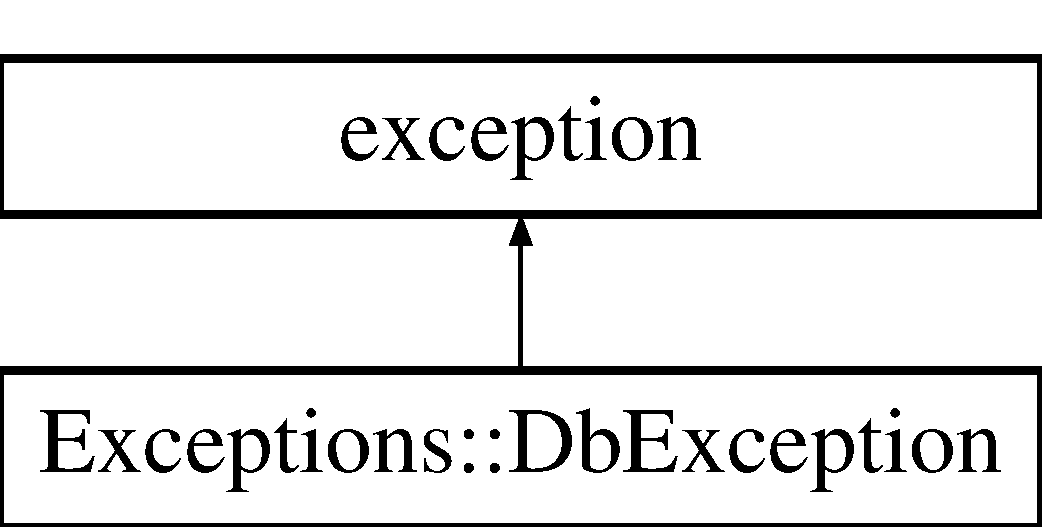
\includegraphics[height=2.000000cm]{d4/de4/classExceptions_1_1DbException}
\end{center}
\end{figure}
\subsection*{Public Member Functions}
\begin{DoxyCompactItemize}
\item 
\hyperlink{classExceptions_1_1DbException_a1e5736082ac86ff18556f66e86f92f58}{Db\-Exception} (const Q\-String fct, const Q\-String fct\-Name, const Q\-String log\-Error, float error\-Code)
\begin{DoxyCompactList}\small\item\em \hyperlink{classExceptions_1_1DbException_a1e5736082ac86ff18556f66e86f92f58}{Db\-Exception\-::\-Db\-Exception}. Construct a \hyperlink{classExceptions_1_1DbException}{Db\-Exception}. \end{DoxyCompactList}\item 
\hypertarget{classExceptions_1_1DbException_ad82383b348d70958ec498ffb73f816ae}{virtual \hyperlink{classExceptions_1_1DbException_ad82383b348d70958ec498ffb73f816ae}{$\sim$\-Db\-Exception} ()  throw ()}\label{classExceptions_1_1DbException_ad82383b348d70958ec498ffb73f816ae}

\begin{DoxyCompactList}\small\item\em $\sim$\-Db\-Exception \end{DoxyCompactList}\item 
void \hyperlink{classExceptions_1_1DbException_a4c04dbebd510cb3206b0263bc57c9f6d}{popup\-Message} (Q\-Widget $\ast$parent)
\begin{DoxyCompactList}\small\item\em \hyperlink{classExceptions_1_1DbException_a4c04dbebd510cb3206b0263bc57c9f6d}{Db\-Exception\-::popup\-Message}. Display a popup message with the message error. \end{DoxyCompactList}\end{DoxyCompactItemize}


\subsection{Detailed Description}
The \hyperlink{classExceptions_1_1DbException}{Db\-Exception} class for database exception \-: queries, db file, … 

\begin{DoxyAuthor}{Author}
Antoine de Roquemaurel 
\end{DoxyAuthor}


\subsection{Constructor \& Destructor Documentation}
\hypertarget{classExceptions_1_1DbException_a1e5736082ac86ff18556f66e86f92f58}{\index{Exceptions\-::\-Db\-Exception@{Exceptions\-::\-Db\-Exception}!Db\-Exception@{Db\-Exception}}
\index{Db\-Exception@{Db\-Exception}!Exceptions::DbException@{Exceptions\-::\-Db\-Exception}}
\subsubsection[{Db\-Exception}]{\setlength{\rightskip}{0pt plus 5cm}Exceptions\-::\-Db\-Exception\-::\-Db\-Exception (
\begin{DoxyParamCaption}
\item[{const Q\-String}]{fct, }
\item[{const Q\-String}]{fct\-Name, }
\item[{const Q\-String}]{log\-Error, }
\item[{float}]{error\-Code}
\end{DoxyParamCaption}
)}}\label{classExceptions_1_1DbException_a1e5736082ac86ff18556f66e86f92f58}


\hyperlink{classExceptions_1_1DbException_a1e5736082ac86ff18556f66e86f92f58}{Db\-Exception\-::\-Db\-Exception}. Construct a \hyperlink{classExceptions_1_1DbException}{Db\-Exception}. 


\begin{DoxyParams}{Parameters}
{\em user\-Error} & Class\-Name of error \\
\hline
{\em fct\-Name} & Function name \\
\hline
{\em log\-Error} & Message error \\
\hline
{\em error\-Code} & Code of error \\
\hline
\end{DoxyParams}


\subsection{Member Function Documentation}
\hypertarget{classExceptions_1_1DbException_a4c04dbebd510cb3206b0263bc57c9f6d}{\index{Exceptions\-::\-Db\-Exception@{Exceptions\-::\-Db\-Exception}!popup\-Message@{popup\-Message}}
\index{popup\-Message@{popup\-Message}!Exceptions::DbException@{Exceptions\-::\-Db\-Exception}}
\subsubsection[{popup\-Message}]{\setlength{\rightskip}{0pt plus 5cm}void Exceptions\-::\-Db\-Exception\-::popup\-Message (
\begin{DoxyParamCaption}
\item[{Q\-Widget $\ast$}]{parent}
\end{DoxyParamCaption}
)}}\label{classExceptions_1_1DbException_a4c04dbebd510cb3206b0263bc57c9f6d}


\hyperlink{classExceptions_1_1DbException_a4c04dbebd510cb3206b0263bc57c9f6d}{Db\-Exception\-::popup\-Message}. Display a popup message with the message error. 


\begin{DoxyParams}{Parameters}
{\em parent} & \\
\hline
\end{DoxyParams}


The documentation for this class was generated from the following files\-:\begin{DoxyCompactItemize}
\item 
/home/travis/build/\-F\-A\-C\-T-\/\-Team/\-Fact\-Dev/src/exceptions/dbexception.\-h\item 
/home/travis/build/\-F\-A\-C\-T-\/\-Team/\-Fact\-Dev/src/exceptions/dbexception.\-cpp\end{DoxyCompactItemize}

\hypertarget{classGui_1_1Dialogs_1_1DialogAddCustomer}{}\section{Gui\+:\+:Dialogs\+:\+:Dialog\+Add\+Customer Class Reference}
\label{classGui_1_1Dialogs_1_1DialogAddCustomer}\index{Gui\+::\+Dialogs\+::\+Dialog\+Add\+Customer@{Gui\+::\+Dialogs\+::\+Dialog\+Add\+Customer}}


The \hyperlink{classGui_1_1Dialogs_1_1DialogAddCustomer}{Dialog\+Add\+Customer} class Window to add or modify a Customer.  




{\ttfamily \#include $<$dialogaddcustomer.\+h$>$}

Inheritance diagram for Gui\+:\+:Dialogs\+:\+:Dialog\+Add\+Customer\+:\begin{figure}[H]
\begin{center}
\leavevmode
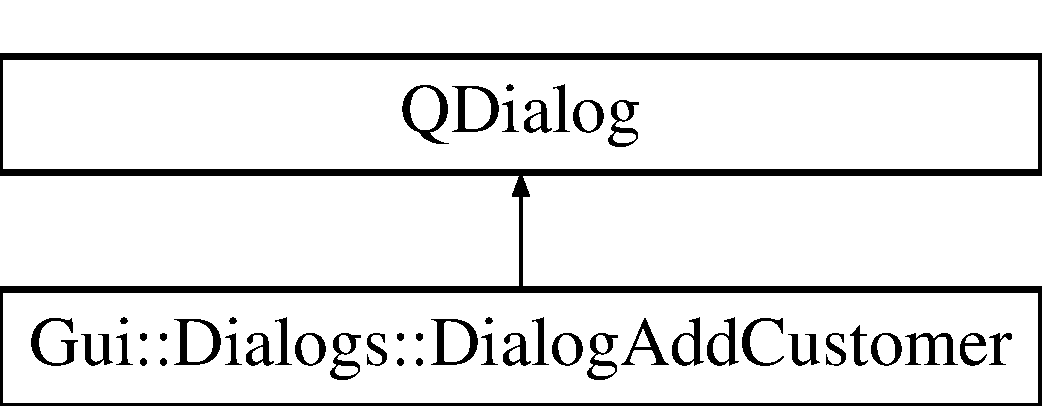
\includegraphics[height=2.000000cm]{d2/d50/classGui_1_1Dialogs_1_1DialogAddCustomer}
\end{center}
\end{figure}
\subsection*{Public Slots}
\begin{DoxyCompactItemize}
\item 
\hypertarget{classGui_1_1Dialogs_1_1DialogAddCustomer_ab1c4fdf53139a3aac7243c42881d2af1}{}void \hyperlink{classGui_1_1Dialogs_1_1DialogAddCustomer_ab1c4fdf53139a3aac7243c42881d2af1}{check\+Fields} ()\label{classGui_1_1Dialogs_1_1DialogAddCustomer_ab1c4fdf53139a3aac7243c42881d2af1}

\begin{DoxyCompactList}\small\item\em \hyperlink{classGui_1_1Dialogs_1_1DialogAddCustomer_ab1c4fdf53139a3aac7243c42881d2af1}{Dialog\+Add\+Customer\+::check\+Fields} Check if fields are valid. \end{DoxyCompactList}\end{DoxyCompactItemize}
\subsection*{Public Member Functions}
\begin{DoxyCompactItemize}
\item 
\hyperlink{classGui_1_1Dialogs_1_1DialogAddCustomer_a7ac689e5bcf3c4e28426016b5a2f1478}{Dialog\+Add\+Customer} (int id=0, Q\+Widget $\ast$parent=0)
\begin{DoxyCompactList}\small\item\em \hyperlink{classGui_1_1Dialogs_1_1DialogAddCustomer_a7ac689e5bcf3c4e28426016b5a2f1478}{Dialog\+Add\+Customer\+::\+Dialog\+Add\+Customer} Construct a window to add/modify a Customer. \end{DoxyCompactList}\item 
\hypertarget{classGui_1_1Dialogs_1_1DialogAddCustomer_a25d53880ea053c960ee621fec29afb36}{}void \hyperlink{classGui_1_1Dialogs_1_1DialogAddCustomer_a25d53880ea053c960ee621fec29afb36}{fill\+Fields} ()\label{classGui_1_1Dialogs_1_1DialogAddCustomer_a25d53880ea053c960ee621fec29afb36}

\begin{DoxyCompactList}\small\item\em \hyperlink{classGui_1_1Dialogs_1_1DialogAddCustomer_a25d53880ea053c960ee621fec29afb36}{Dialog\+Add\+Customer\+::fill\+Fields} If the Customer exits, fill line edits with the data of the current Customer. \end{DoxyCompactList}\item 
\hypertarget{classGui_1_1Dialogs_1_1DialogAddCustomer_ab9f488af3fdfbf0ca9851cc59946dd5d}{}void \hyperlink{classGui_1_1Dialogs_1_1DialogAddCustomer_ab9f488af3fdfbf0ca9851cc59946dd5d}{accept} ()\label{classGui_1_1Dialogs_1_1DialogAddCustomer_ab9f488af3fdfbf0ca9851cc59946dd5d}

\begin{DoxyCompactList}\small\item\em \hyperlink{classGui_1_1Dialogs_1_1DialogAddCustomer_ab9f488af3fdfbf0ca9851cc59946dd5d}{Dialog\+Add\+Customer\+::accept} Valid data inputed by user and add these data in Database. \end{DoxyCompactList}\item 
\hypertarget{classGui_1_1Dialogs_1_1DialogAddCustomer_a5f3b96e858dedc8a54ff184baafd6e90}{}void \hyperlink{classGui_1_1Dialogs_1_1DialogAddCustomer_a5f3b96e858dedc8a54ff184baafd6e90}{reject} ()\label{classGui_1_1Dialogs_1_1DialogAddCustomer_a5f3b96e858dedc8a54ff184baafd6e90}

\begin{DoxyCompactList}\small\item\em \hyperlink{classGui_1_1Dialogs_1_1DialogAddCustomer_a5f3b96e858dedc8a54ff184baafd6e90}{Dialog\+Add\+Customer\+::reject} Cancel the operation and close the windows. \end{DoxyCompactList}\end{DoxyCompactItemize}


\subsection{Detailed Description}
The \hyperlink{classGui_1_1Dialogs_1_1DialogAddCustomer}{Dialog\+Add\+Customer} class Window to add or modify a Customer. 

\begin{DoxyAuthor}{Author}

\end{DoxyAuthor}


\subsection{Constructor \& Destructor Documentation}
\hypertarget{classGui_1_1Dialogs_1_1DialogAddCustomer_a7ac689e5bcf3c4e28426016b5a2f1478}{}\index{Gui\+::\+Dialogs\+::\+Dialog\+Add\+Customer@{Gui\+::\+Dialogs\+::\+Dialog\+Add\+Customer}!Dialog\+Add\+Customer@{Dialog\+Add\+Customer}}
\index{Dialog\+Add\+Customer@{Dialog\+Add\+Customer}!Gui\+::\+Dialogs\+::\+Dialog\+Add\+Customer@{Gui\+::\+Dialogs\+::\+Dialog\+Add\+Customer}}
\subsubsection[{Dialog\+Add\+Customer}]{\setlength{\rightskip}{0pt plus 5cm}Gui\+::\+Dialogs\+::\+Dialog\+Add\+Customer\+::\+Dialog\+Add\+Customer (
\begin{DoxyParamCaption}
\item[{int}]{id = {\ttfamily 0}, }
\item[{Q\+Widget $\ast$}]{parent = {\ttfamily 0}}
\end{DoxyParamCaption}
)\hspace{0.3cm}{\ttfamily [explicit]}}\label{classGui_1_1Dialogs_1_1DialogAddCustomer_a7ac689e5bcf3c4e28426016b5a2f1478}


\hyperlink{classGui_1_1Dialogs_1_1DialogAddCustomer_a7ac689e5bcf3c4e28426016b5a2f1478}{Dialog\+Add\+Customer\+::\+Dialog\+Add\+Customer} Construct a window to add/modify a Customer. 


\begin{DoxyParams}{Parameters}
{\em id} & Customer id \\
\hline
{\em parent} & Q\+Widget parent \\
\hline
\end{DoxyParams}


The documentation for this class was generated from the following files\+:\begin{DoxyCompactItemize}
\item 
src/gui/dialogs/dialogaddcustomer.\+h\item 
src/gui/dialogs/dialogaddcustomer.\+cpp\end{DoxyCompactItemize}

\hypertarget{classICheckField}{\section{I\+Check\+Field Class Reference}
\label{classICheckField}\index{I\+Check\+Field@{I\+Check\+Field}}
}


The \hyperlink{classICheckField}{I\+Check\+Field} class Interface to check fields validity.  




{\ttfamily \#include $<$icheckfield.\+h$>$}

Inheritance diagram for I\+Check\+Field\+:\begin{figure}[H]
\begin{center}
\leavevmode
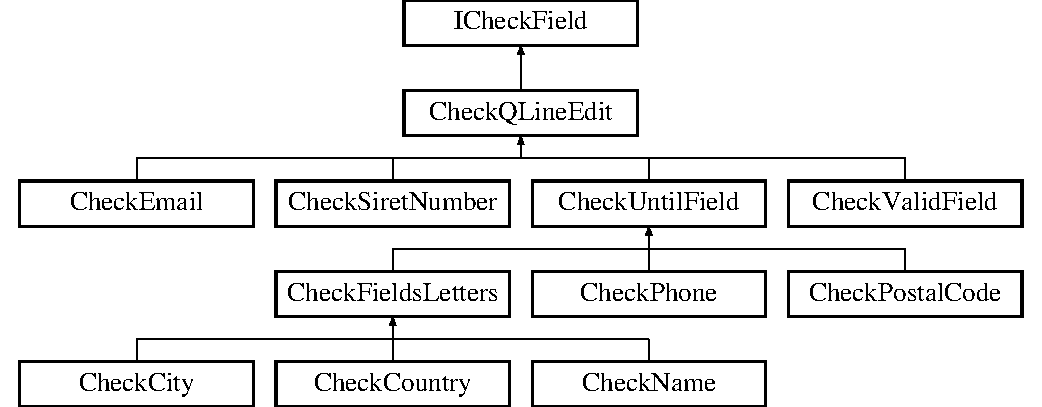
\includegraphics[height=5.000000cm]{d5/d75/classICheckField}
\end{center}
\end{figure}
\subsection*{Public Member Functions}
\begin{DoxyCompactItemize}
\item 
virtual bool \hyperlink{classICheckField_a6bd42b4d49c165cdd92822135123fd4b}{check} (Q\+String text)=0
\begin{DoxyCompactList}\small\item\em check Check if the field (line edit) is valid Return T\+R\+U\+E if the field is valid, else F\+A\+L\+S\+E \end{DoxyCompactList}\end{DoxyCompactItemize}


\subsection{Detailed Description}
The \hyperlink{classICheckField}{I\+Check\+Field} class Interface to check fields validity. 

\subsection{Member Function Documentation}
\hypertarget{classICheckField_a6bd42b4d49c165cdd92822135123fd4b}{\index{I\+Check\+Field@{I\+Check\+Field}!check@{check}}
\index{check@{check}!I\+Check\+Field@{I\+Check\+Field}}
\subsubsection[{check}]{\setlength{\rightskip}{0pt plus 5cm}virtual bool I\+Check\+Field\+::check (
\begin{DoxyParamCaption}
\item[{Q\+String}]{text}
\end{DoxyParamCaption}
)\hspace{0.3cm}{\ttfamily [pure virtual]}}}\label{classICheckField_a6bd42b4d49c165cdd92822135123fd4b}


check Check if the field (line edit) is valid Return T\+R\+U\+E if the field is valid, else F\+A\+L\+S\+E 

\begin{DoxyReturn}{Returns}
boolean 
\end{DoxyReturn}


Implemented in \hyperlink{classCheckEmail_a544d7656d36bd463391fe2f4dd3e13c6}{Check\+Email}, \hyperlink{classCheckPhone_ac60f1428fc89e1b2630db022e14509ed}{Check\+Phone}, \hyperlink{classCheckPostalCode_ad91ba5622617675fbb5c767036163142}{Check\+Postal\+Code}, \hyperlink{classCheckSiretNumber_aaf0a1411e380789062564bd992e72c1b}{Check\+Siret\+Number}, \hyperlink{classCheckUntilField_acfb9e2f95bebcb5b5d2337e3ac4f4d47}{Check\+Until\+Field}, \hyperlink{classCheckFieldsLetters_a62574deb407fe83456e46381425a7b46}{Check\+Fields\+Letters}, and \hyperlink{classCheckValidField_a192b1c9c84ea8897661425fd3c0b9e8e}{Check\+Valid\+Field}.



The documentation for this class was generated from the following file\+:\begin{DoxyCompactItemize}
\item 
src/gui/widgets/checkfields/icheckfield.\+h\end{DoxyCompactItemize}

\hypertarget{classModels_1_1IDatabaseModel}{\section{Models\+:\+:I\+Database\+Model Class Reference}
\label{classModels_1_1IDatabaseModel}\index{Models\+::\+I\+Database\+Model@{Models\+::\+I\+Database\+Model}}
}


The \hyperlink{classModels_1_1IDatabaseModel}{I\+Database\+Model} class.  




{\ttfamily \#include $<$idatabasemodel.\+h$>$}

Inheritance diagram for Models\+:\+:I\+Database\+Model\+:\begin{figure}[H]
\begin{center}
\leavevmode
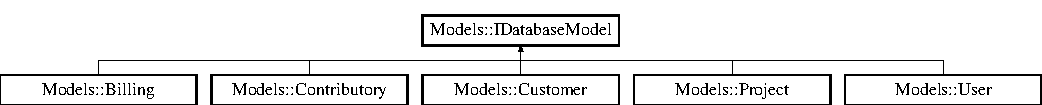
\includegraphics[height=1.417722cm]{df/ddd/classModels_1_1IDatabaseModel}
\end{center}
\end{figure}
\subsection*{Public Member Functions}
\begin{DoxyCompactItemize}
\item 
\hypertarget{classModels_1_1IDatabaseModel_a7dd56f574720919d1703651f5896141f}{virtual \hyperlink{classModels_1_1IDatabaseModel_a7dd56f574720919d1703651f5896141f}{$\sim$\+I\+Database\+Model} ()}\label{classModels_1_1IDatabaseModel_a7dd56f574720919d1703651f5896141f}

\begin{DoxyCompactList}\small\item\em $\sim$\+I\+Database\+Model Remove an instance of \hyperlink{classModels_1_1IDatabaseModel}{I\+Database\+Model} \end{DoxyCompactList}\item 
\hypertarget{classModels_1_1IDatabaseModel_a8fcb1587824753cd121a7d961b60a98a}{virtual void \hyperlink{classModels_1_1IDatabaseModel_a8fcb1587824753cd121a7d961b60a98a}{commit} ()=0}\label{classModels_1_1IDatabaseModel_a8fcb1587824753cd121a7d961b60a98a}

\begin{DoxyCompactList}\small\item\em \hyperlink{classModels_1_1IDatabaseModel_a8fcb1587824753cd121a7d961b60a98a}{I\+Database\+Model\+::commit} Update or insert data into the database. \end{DoxyCompactList}\item 
virtual void \hyperlink{classModels_1_1IDatabaseModel_af0814d81fc76a881bc64d9062adf1f6c}{hydrat} (int id)=0
\begin{DoxyCompactList}\small\item\em \hyperlink{classModels_1_1IDatabaseModel_af0814d81fc76a881bc64d9062adf1f6c}{I\+Database\+Model\+::hydrat} Get data of the element which is specified by the identify {\itshape id} from the database. \end{DoxyCompactList}\item 
\hypertarget{classModels_1_1IDatabaseModel_a6d8eca5b493b57c21feafae75c783b14}{virtual void \hyperlink{classModels_1_1IDatabaseModel_a6d8eca5b493b57c21feafae75c783b14}{remove} ()=0}\label{classModels_1_1IDatabaseModel_a6d8eca5b493b57c21feafae75c783b14}

\begin{DoxyCompactList}\small\item\em \hyperlink{classModels_1_1IDatabaseModel_a6d8eca5b493b57c21feafae75c783b14}{I\+Database\+Model\+::remove} Remove the current element in the database. \end{DoxyCompactList}\item 
int \hyperlink{classModels_1_1IDatabaseModel_a6a4d1d3c0912c97c61a9d4de7471afee}{get\+Id} () const 
\begin{DoxyCompactList}\small\item\em \hyperlink{classModels_1_1IDatabaseModel_a6a4d1d3c0912c97c61a9d4de7471afee}{I\+Database\+Model\+::get\+Id} Return the identify of the element of the database. \end{DoxyCompactList}\item 
void \hyperlink{classModels_1_1IDatabaseModel_a6bf2ec005b5d931e58ee8125e92d9722}{set\+Id} (int id)
\begin{DoxyCompactList}\small\item\em \hyperlink{classModels_1_1IDatabaseModel_a6bf2ec005b5d931e58ee8125e92d9722}{I\+Database\+Model\+::set\+Id} Replace the current identify by {\itshape id} \end{DoxyCompactList}\item 
bool \hyperlink{classModels_1_1IDatabaseModel_a058e5b85d95e9424245dc37eb122350c}{is\+To\+Removed} () const 
\begin{DoxyCompactList}\small\item\em to\+Removed return if object must be removed. \end{DoxyCompactList}\item 
void \hyperlink{classModels_1_1IDatabaseModel_ac399b44ba1178ef6f54da31203e11d9f}{set\+To\+Removed} (bool to\+Removed)
\begin{DoxyCompactList}\small\item\em set\+To\+Removed Change the flag for removed object \end{DoxyCompactList}\end{DoxyCompactItemize}
\subsection*{Protected Attributes}
\begin{DoxyCompactItemize}
\item 
\hypertarget{classModels_1_1IDatabaseModel_a85fbc8298dee2e84f310a21ed935665f}{int \hyperlink{classModels_1_1IDatabaseModel_a85fbc8298dee2e84f310a21ed935665f}{\+\_\+id}}\label{classModels_1_1IDatabaseModel_a85fbc8298dee2e84f310a21ed935665f}

\begin{DoxyCompactList}\small\item\em Element identify. \end{DoxyCompactList}\item 
\hypertarget{classModels_1_1IDatabaseModel_acfa9af965e01f44d6ff75226e23e4640}{bool \hyperlink{classModels_1_1IDatabaseModel_acfa9af965e01f44d6ff75226e23e4640}{\+\_\+to\+Removed}}\label{classModels_1_1IDatabaseModel_acfa9af965e01f44d6ff75226e23e4640}

\begin{DoxyCompactList}\small\item\em Flag to know if the object must be removed. \end{DoxyCompactList}\end{DoxyCompactItemize}


\subsection{Detailed Description}
The \hyperlink{classModels_1_1IDatabaseModel}{I\+Database\+Model} class. 

\begin{DoxyAuthor}{Author}
Antoine de Roquemaurel 
\end{DoxyAuthor}


\subsection{Member Function Documentation}
\hypertarget{classModels_1_1IDatabaseModel_a6a4d1d3c0912c97c61a9d4de7471afee}{\index{Models\+::\+I\+Database\+Model@{Models\+::\+I\+Database\+Model}!get\+Id@{get\+Id}}
\index{get\+Id@{get\+Id}!Models\+::\+I\+Database\+Model@{Models\+::\+I\+Database\+Model}}
\subsubsection[{get\+Id}]{\setlength{\rightskip}{0pt plus 5cm}int Models\+::\+I\+Database\+Model\+::get\+Id (
\begin{DoxyParamCaption}
{}
\end{DoxyParamCaption}
) const\hspace{0.3cm}{\ttfamily [inline]}}}\label{classModels_1_1IDatabaseModel_a6a4d1d3c0912c97c61a9d4de7471afee}


\hyperlink{classModels_1_1IDatabaseModel_a6a4d1d3c0912c97c61a9d4de7471afee}{I\+Database\+Model\+::get\+Id} Return the identify of the element of the database. 

\begin{DoxyReturn}{Returns}
identity 
\end{DoxyReturn}
\hypertarget{classModels_1_1IDatabaseModel_af0814d81fc76a881bc64d9062adf1f6c}{\index{Models\+::\+I\+Database\+Model@{Models\+::\+I\+Database\+Model}!hydrat@{hydrat}}
\index{hydrat@{hydrat}!Models\+::\+I\+Database\+Model@{Models\+::\+I\+Database\+Model}}
\subsubsection[{hydrat}]{\setlength{\rightskip}{0pt plus 5cm}virtual void Models\+::\+I\+Database\+Model\+::hydrat (
\begin{DoxyParamCaption}
\item[{int}]{id}
\end{DoxyParamCaption}
)\hspace{0.3cm}{\ttfamily [pure virtual]}}}\label{classModels_1_1IDatabaseModel_af0814d81fc76a881bc64d9062adf1f6c}


\hyperlink{classModels_1_1IDatabaseModel_af0814d81fc76a881bc64d9062adf1f6c}{I\+Database\+Model\+::hydrat} Get data of the element which is specified by the identify {\itshape id} from the database. 


\begin{DoxyParams}{Parameters}
{\em id} & \\
\hline
\end{DoxyParams}


Implemented in \hyperlink{classModels_1_1Project_aa293709eeb68e4271cac8d4cce418ffa}{Models\+::\+Project}, \hyperlink{classModels_1_1Billing_a689643008955fdcd5833631a6202c0dc}{Models\+::\+Billing}, \hyperlink{classModels_1_1Contributory_a40248b5853045eb46412396513f36b06}{Models\+::\+Contributory}, \hyperlink{classModels_1_1User_ab46c7e1841dca66bc01cd95328b97877}{Models\+::\+User}, and \hyperlink{classModels_1_1Customer_afe3ed7fb893d61ea6f4d14e73779382c}{Models\+::\+Customer}.

\hypertarget{classModels_1_1IDatabaseModel_a058e5b85d95e9424245dc37eb122350c}{\index{Models\+::\+I\+Database\+Model@{Models\+::\+I\+Database\+Model}!is\+To\+Removed@{is\+To\+Removed}}
\index{is\+To\+Removed@{is\+To\+Removed}!Models\+::\+I\+Database\+Model@{Models\+::\+I\+Database\+Model}}
\subsubsection[{is\+To\+Removed}]{\setlength{\rightskip}{0pt plus 5cm}bool Models\+::\+I\+Database\+Model\+::is\+To\+Removed (
\begin{DoxyParamCaption}
{}
\end{DoxyParamCaption}
) const\hspace{0.3cm}{\ttfamily [inline]}}}\label{classModels_1_1IDatabaseModel_a058e5b85d95e9424245dc37eb122350c}


to\+Removed return if object must be removed. 

\begin{DoxyReturn}{Returns}

\end{DoxyReturn}
\hypertarget{classModels_1_1IDatabaseModel_a6bf2ec005b5d931e58ee8125e92d9722}{\index{Models\+::\+I\+Database\+Model@{Models\+::\+I\+Database\+Model}!set\+Id@{set\+Id}}
\index{set\+Id@{set\+Id}!Models\+::\+I\+Database\+Model@{Models\+::\+I\+Database\+Model}}
\subsubsection[{set\+Id}]{\setlength{\rightskip}{0pt plus 5cm}void Models\+::\+I\+Database\+Model\+::set\+Id (
\begin{DoxyParamCaption}
\item[{int}]{id}
\end{DoxyParamCaption}
)\hspace{0.3cm}{\ttfamily [inline]}}}\label{classModels_1_1IDatabaseModel_a6bf2ec005b5d931e58ee8125e92d9722}


\hyperlink{classModels_1_1IDatabaseModel_a6bf2ec005b5d931e58ee8125e92d9722}{I\+Database\+Model\+::set\+Id} Replace the current identify by {\itshape id} 


\begin{DoxyParams}{Parameters}
{\em id} & New identify \\
\hline
\end{DoxyParams}
\hypertarget{classModels_1_1IDatabaseModel_ac399b44ba1178ef6f54da31203e11d9f}{\index{Models\+::\+I\+Database\+Model@{Models\+::\+I\+Database\+Model}!set\+To\+Removed@{set\+To\+Removed}}
\index{set\+To\+Removed@{set\+To\+Removed}!Models\+::\+I\+Database\+Model@{Models\+::\+I\+Database\+Model}}
\subsubsection[{set\+To\+Removed}]{\setlength{\rightskip}{0pt plus 5cm}void Models\+::\+I\+Database\+Model\+::set\+To\+Removed (
\begin{DoxyParamCaption}
\item[{bool}]{to\+Removed}
\end{DoxyParamCaption}
)\hspace{0.3cm}{\ttfamily [inline]}}}\label{classModels_1_1IDatabaseModel_ac399b44ba1178ef6f54da31203e11d9f}


set\+To\+Removed Change the flag for removed object 


\begin{DoxyParams}{Parameters}
{\em to\+Removed} & The new flag \\
\hline
\end{DoxyParams}


The documentation for this class was generated from the following file\+:\begin{DoxyCompactItemize}
\item 
src/models/idatabasemodel.\+h\end{DoxyCompactItemize}

\hypertarget{classUtils_1_1ItemType}{\section{Utils\-:\-:Item\-Type Class Reference}
\label{classUtils_1_1ItemType}\index{Utils\-::\-Item\-Type@{Utils\-::\-Item\-Type}}
}


The \hyperlink{classUtils_1_1ItemType}{Item\-Type} class Item type model.  




{\ttfamily \#include $<$itemtype.\-h$>$}

\subsection*{Public Member Functions}
\begin{DoxyCompactItemize}
\item 
\hyperlink{classUtils_1_1ItemType_a5b06f6c289619f01ced33db7b16ab0f9}{Item\-Type} (int type, Q\-String name)
\begin{DoxyCompactList}\small\item\em \hyperlink{classUtils_1_1ItemType_a5b06f6c289619f01ced33db7b16ab0f9}{Item\-Type\-::\-Item\-Type} Construct an Item type. \end{DoxyCompactList}\item 
Q\-String \hyperlink{classUtils_1_1ItemType_a09fdb09837ad0ab678a271d3f97dd006}{get\-Name} () const 
\begin{DoxyCompactList}\small\item\em \hyperlink{classUtils_1_1ItemType_a09fdb09837ad0ab678a271d3f97dd006}{Item\-Type\-::get\-Name} Get item name. \end{DoxyCompactList}\item 
\hyperlink{classModels_1_1IModel}{Models\-::\-I\-Model} $\ast$ \hyperlink{classUtils_1_1ItemType_aff3b98516a4ee741cf926d9cd7cbd131}{get\-Model} (int id)
\begin{DoxyCompactList}\small\item\em \hyperlink{classUtils_1_1ItemType_aff3b98516a4ee741cf926d9cd7cbd131}{Item\-Type\-::get\-Model} Get the databasemodele of the {\bfseries \hyperlink{classUtils_1_1ItemType}{Item\-Type}} according to this identity {\itshape id} \end{DoxyCompactList}\item 
void \hyperlink{classUtils_1_1ItemType_aa993c315def3988851fc3af5f826c384}{set\-Name} (const Q\-String \&name)
\begin{DoxyCompactList}\small\item\em \hyperlink{classUtils_1_1ItemType_aa993c315def3988851fc3af5f826c384}{Item\-Type\-::set\-Name} Modify the item name. \end{DoxyCompactList}\item 
int \hyperlink{classUtils_1_1ItemType_a83266bf1a7fecbc0e747c5dc2b079ff5}{get\-Type} () const 
\begin{DoxyCompactList}\small\item\em \hyperlink{classUtils_1_1ItemType_a83266bf1a7fecbc0e747c5dc2b079ff5}{Item\-Type\-::get\-Type} Get the type of the current item. \end{DoxyCompactList}\item 
void \hyperlink{classUtils_1_1ItemType_a80b89017d22b33c1ac1c84055592b7f7}{set\-Type} (int type)
\begin{DoxyCompactList}\small\item\em \hyperlink{classUtils_1_1ItemType_a80b89017d22b33c1ac1c84055592b7f7}{Item\-Type\-::set\-Type} Modify the type of the current item. \end{DoxyCompactList}\end{DoxyCompactItemize}
\subsection*{Static Public Attributes}
\begin{DoxyCompactItemize}
\item 
\hypertarget{classUtils_1_1ItemType_a181d6656c7e2db09962fda0925c38ea5}{static const int \hyperlink{classUtils_1_1ItemType_a181d6656c7e2db09962fda0925c38ea5}{C\-U\-S\-T\-O\-M\-E\-R} = 0}\label{classUtils_1_1ItemType_a181d6656c7e2db09962fda0925c38ea5}

\begin{DoxyCompactList}\small\item\em constant value assigned to Customer \end{DoxyCompactList}\item 
\hypertarget{classUtils_1_1ItemType_aa3f6eae0de61e9c259dae988c1e13846}{static const int \hyperlink{classUtils_1_1ItemType_aa3f6eae0de61e9c259dae988c1e13846}{P\-R\-O\-J\-E\-C\-T} = 1}\label{classUtils_1_1ItemType_aa3f6eae0de61e9c259dae988c1e13846}

\begin{DoxyCompactList}\small\item\em constant value assigned to Project \end{DoxyCompactList}\item 
\hypertarget{classUtils_1_1ItemType_a21c22e857bbe4549f37e3ae4e34c4ede}{static const int \hyperlink{classUtils_1_1ItemType_a21c22e857bbe4549f37e3ae4e34c4ede}{B\-I\-L\-L\-I\-N\-G} = 2}\label{classUtils_1_1ItemType_a21c22e857bbe4549f37e3ae4e34c4ede}

\begin{DoxyCompactList}\small\item\em constant value assigned to Billing \end{DoxyCompactList}\item 
\hypertarget{classUtils_1_1ItemType_a5c34781b4518fed7d53ce6f9aa4911c8}{static const int \hyperlink{classUtils_1_1ItemType_a5c34781b4518fed7d53ce6f9aa4911c8}{Q\-U\-O\-T\-E} = 3}\label{classUtils_1_1ItemType_a5c34781b4518fed7d53ce6f9aa4911c8}

\begin{DoxyCompactList}\small\item\em constant value assigned to Quote \end{DoxyCompactList}\end{DoxyCompactItemize}


\subsection{Detailed Description}
The \hyperlink{classUtils_1_1ItemType}{Item\-Type} class Item type model. 

\subsection{Constructor \& Destructor Documentation}
\hypertarget{classUtils_1_1ItemType_a5b06f6c289619f01ced33db7b16ab0f9}{\index{Utils\-::\-Item\-Type@{Utils\-::\-Item\-Type}!Item\-Type@{Item\-Type}}
\index{Item\-Type@{Item\-Type}!Utils::ItemType@{Utils\-::\-Item\-Type}}
\subsubsection[{Item\-Type}]{\setlength{\rightskip}{0pt plus 5cm}Utils\-::\-Item\-Type\-::\-Item\-Type (
\begin{DoxyParamCaption}
\item[{int}]{type, }
\item[{Q\-String}]{name}
\end{DoxyParamCaption}
)}}\label{classUtils_1_1ItemType_a5b06f6c289619f01ced33db7b16ab0f9}


\hyperlink{classUtils_1_1ItemType_a5b06f6c289619f01ced33db7b16ab0f9}{Item\-Type\-::\-Item\-Type} Construct an Item type. 


\begin{DoxyParams}{Parameters}
{\em type} & Type of the item \\
\hline
{\em name} & Name of the item \\
\hline
\end{DoxyParams}


\subsection{Member Function Documentation}
\hypertarget{classUtils_1_1ItemType_aff3b98516a4ee741cf926d9cd7cbd131}{\index{Utils\-::\-Item\-Type@{Utils\-::\-Item\-Type}!get\-Model@{get\-Model}}
\index{get\-Model@{get\-Model}!Utils::ItemType@{Utils\-::\-Item\-Type}}
\subsubsection[{get\-Model}]{\setlength{\rightskip}{0pt plus 5cm}{\bf Models\-::\-I\-Model} $\ast$ Utils\-::\-Item\-Type\-::get\-Model (
\begin{DoxyParamCaption}
\item[{int}]{id}
\end{DoxyParamCaption}
)}}\label{classUtils_1_1ItemType_aff3b98516a4ee741cf926d9cd7cbd131}


\hyperlink{classUtils_1_1ItemType_aff3b98516a4ee741cf926d9cd7cbd131}{Item\-Type\-::get\-Model} Get the databasemodele of the {\bfseries \hyperlink{classUtils_1_1ItemType}{Item\-Type}} according to this identity {\itshape id} 


\begin{DoxyParams}{Parameters}
{\em id} & Item type identity \\
\hline
\end{DoxyParams}
\begin{DoxyReturn}{Returns}
database model 
\end{DoxyReturn}
\hypertarget{classUtils_1_1ItemType_a09fdb09837ad0ab678a271d3f97dd006}{\index{Utils\-::\-Item\-Type@{Utils\-::\-Item\-Type}!get\-Name@{get\-Name}}
\index{get\-Name@{get\-Name}!Utils::ItemType@{Utils\-::\-Item\-Type}}
\subsubsection[{get\-Name}]{\setlength{\rightskip}{0pt plus 5cm}Q\-String Utils\-::\-Item\-Type\-::get\-Name (
\begin{DoxyParamCaption}
{}
\end{DoxyParamCaption}
) const}}\label{classUtils_1_1ItemType_a09fdb09837ad0ab678a271d3f97dd006}


\hyperlink{classUtils_1_1ItemType_a09fdb09837ad0ab678a271d3f97dd006}{Item\-Type\-::get\-Name} Get item name. 

\begin{DoxyReturn}{Returns}
item name 
\end{DoxyReturn}
\hypertarget{classUtils_1_1ItemType_a83266bf1a7fecbc0e747c5dc2b079ff5}{\index{Utils\-::\-Item\-Type@{Utils\-::\-Item\-Type}!get\-Type@{get\-Type}}
\index{get\-Type@{get\-Type}!Utils::ItemType@{Utils\-::\-Item\-Type}}
\subsubsection[{get\-Type}]{\setlength{\rightskip}{0pt plus 5cm}int Utils\-::\-Item\-Type\-::get\-Type (
\begin{DoxyParamCaption}
{}
\end{DoxyParamCaption}
) const}}\label{classUtils_1_1ItemType_a83266bf1a7fecbc0e747c5dc2b079ff5}


\hyperlink{classUtils_1_1ItemType_a83266bf1a7fecbc0e747c5dc2b079ff5}{Item\-Type\-::get\-Type} Get the type of the current item. 

\begin{DoxyReturn}{Returns}
type of the current item 
\end{DoxyReturn}
\hypertarget{classUtils_1_1ItemType_aa993c315def3988851fc3af5f826c384}{\index{Utils\-::\-Item\-Type@{Utils\-::\-Item\-Type}!set\-Name@{set\-Name}}
\index{set\-Name@{set\-Name}!Utils::ItemType@{Utils\-::\-Item\-Type}}
\subsubsection[{set\-Name}]{\setlength{\rightskip}{0pt plus 5cm}void Utils\-::\-Item\-Type\-::set\-Name (
\begin{DoxyParamCaption}
\item[{const Q\-String \&}]{name}
\end{DoxyParamCaption}
)}}\label{classUtils_1_1ItemType_aa993c315def3988851fc3af5f826c384}


\hyperlink{classUtils_1_1ItemType_aa993c315def3988851fc3af5f826c384}{Item\-Type\-::set\-Name} Modify the item name. 


\begin{DoxyParams}{Parameters}
{\em name} & New Item name \\
\hline
\end{DoxyParams}
\hypertarget{classUtils_1_1ItemType_a80b89017d22b33c1ac1c84055592b7f7}{\index{Utils\-::\-Item\-Type@{Utils\-::\-Item\-Type}!set\-Type@{set\-Type}}
\index{set\-Type@{set\-Type}!Utils::ItemType@{Utils\-::\-Item\-Type}}
\subsubsection[{set\-Type}]{\setlength{\rightskip}{0pt plus 5cm}void Utils\-::\-Item\-Type\-::set\-Type (
\begin{DoxyParamCaption}
\item[{int}]{type}
\end{DoxyParamCaption}
)}}\label{classUtils_1_1ItemType_a80b89017d22b33c1ac1c84055592b7f7}


\hyperlink{classUtils_1_1ItemType_a80b89017d22b33c1ac1c84055592b7f7}{Item\-Type\-::set\-Type} Modify the type of the current item. 


\begin{DoxyParams}{Parameters}
{\em type} & New item type \\
\hline
\end{DoxyParams}


The documentation for this class was generated from the following files\-:\begin{DoxyCompactItemize}
\item 
/home/florent/\-Documents/\-Projet\-\_\-\-S8/\-Fact\-Dev/src/utils/itemtype.\-h\item 
/home/florent/\-Documents/\-Projet\-\_\-\-S8/\-Fact\-Dev/src/utils/itemtype.\-cpp\end{DoxyCompactItemize}

\hypertarget{classUtils_1_1Log}{}\section{Utils\+:\+:Log Class Reference}
\label{classUtils_1_1Log}\index{Utils\+::\+Log@{Utils\+::\+Log}}


The \hyperlink{classUtils_1_1Log}{Log} class for Simple management of log.  




{\ttfamily \#include $<$log.\+h$>$}

\subsection*{Public Member Functions}
\begin{DoxyCompactItemize}
\item 
\hypertarget{classUtils_1_1Log_a659ea51c0749983cf9bba0274aa10184}{}\hyperlink{classUtils_1_1Log_a659ea51c0749983cf9bba0274aa10184}{$\sim$\+Log} ()\label{classUtils_1_1Log_a659ea51c0749983cf9bba0274aa10184}

\begin{DoxyCompactList}\small\item\em \hyperlink{classUtils_1_1Log_a659ea51c0749983cf9bba0274aa10184}{Log\+::$\sim$\+Log}. \end{DoxyCompactList}\item 
void \hyperlink{classUtils_1_1Log_a9f21042e13648171da95b27830e91c75}{write} (const Q\+String text)
\begin{DoxyCompactList}\small\item\em \hyperlink{classUtils_1_1Log_a9f21042e13648171da95b27830e91c75}{Log\+::write}. Write log message in file. \end{DoxyCompactList}\item 
\hypertarget{classUtils_1_1Log_a0191645e4f86af331290c7062c79d7b7}{}\hyperlink{classUtils_1_1Log_a0191645e4f86af331290c7062c79d7b7}{Log} ()\label{classUtils_1_1Log_a0191645e4f86af331290c7062c79d7b7}

\begin{DoxyCompactList}\small\item\em \hyperlink{classUtils_1_1Log_a0191645e4f86af331290c7062c79d7b7}{Log\+::\+Log}. \hyperlink{classUtils_1_1Log}{Log} is a singleton. \end{DoxyCompactList}\end{DoxyCompactItemize}
\subsection*{Static Public Member Functions}
\begin{DoxyCompactItemize}
\item 
static \hyperlink{classUtils_1_1Log}{Log} \& \hyperlink{classUtils_1_1Log_aea616362bc63f99499e3964d5dc759d2}{instance} (Type\+Log type=I\+N\+F\+O)
\begin{DoxyCompactList}\small\item\em \hyperlink{classUtils_1_1Log_aea616362bc63f99499e3964d5dc759d2}{Log\+::instance}. Return the instance of logger. \end{DoxyCompactList}\end{DoxyCompactItemize}
\subsection*{Friends}
\begin{DoxyCompactItemize}
\item 
\hyperlink{classUtils_1_1Log}{Log} \& \hyperlink{classUtils_1_1Log_a1ecba3328cadecbbd7d65ae2852171fc}{operator$<$$<$} (\hyperlink{classUtils_1_1Log}{Log} \&logger, const Q\+String \&text)
\begin{DoxyCompactList}\small\item\em operator $<$$<$ for log writing \end{DoxyCompactList}\end{DoxyCompactItemize}


\subsection{Detailed Description}
The \hyperlink{classUtils_1_1Log}{Log} class for Simple management of log. 

\subsection{Member Function Documentation}
\hypertarget{classUtils_1_1Log_aea616362bc63f99499e3964d5dc759d2}{}\index{Utils\+::\+Log@{Utils\+::\+Log}!instance@{instance}}
\index{instance@{instance}!Utils\+::\+Log@{Utils\+::\+Log}}
\subsubsection[{instance}]{\setlength{\rightskip}{0pt plus 5cm}{\bf Log} \& Utils\+::\+Log\+::instance (
\begin{DoxyParamCaption}
\item[{Type\+Log}]{type = {\ttfamily INFO}}
\end{DoxyParamCaption}
)\hspace{0.3cm}{\ttfamily [static]}}\label{classUtils_1_1Log_aea616362bc63f99499e3964d5dc759d2}


\hyperlink{classUtils_1_1Log_aea616362bc63f99499e3964d5dc759d2}{Log\+::instance}. Return the instance of logger. 


\begin{DoxyParams}{Parameters}
{\em type} & Type of log \+: W\+A\+R\+N\+I\+N\+G, I\+N\+F\+O, E\+R\+R\+O\+R \\
\hline
\end{DoxyParams}
\begin{DoxyReturn}{Returns}
Instance of logger. 
\end{DoxyReturn}
\hypertarget{classUtils_1_1Log_a9f21042e13648171da95b27830e91c75}{}\index{Utils\+::\+Log@{Utils\+::\+Log}!write@{write}}
\index{write@{write}!Utils\+::\+Log@{Utils\+::\+Log}}
\subsubsection[{write}]{\setlength{\rightskip}{0pt plus 5cm}void Utils\+::\+Log\+::write (
\begin{DoxyParamCaption}
\item[{const Q\+String}]{text}
\end{DoxyParamCaption}
)}\label{classUtils_1_1Log_a9f21042e13648171da95b27830e91c75}


\hyperlink{classUtils_1_1Log_a9f21042e13648171da95b27830e91c75}{Log\+::write}. Write log message in file. 


\begin{DoxyParams}{Parameters}
{\em text} & \\
\hline
\end{DoxyParams}


\subsection{Friends And Related Function Documentation}
\hypertarget{classUtils_1_1Log_a1ecba3328cadecbbd7d65ae2852171fc}{}\index{Utils\+::\+Log@{Utils\+::\+Log}!operator$<$$<$@{operator$<$$<$}}
\index{operator$<$$<$@{operator$<$$<$}!Utils\+::\+Log@{Utils\+::\+Log}}
\subsubsection[{operator$<$$<$}]{\setlength{\rightskip}{0pt plus 5cm}{\bf Log}\& operator$<$$<$ (
\begin{DoxyParamCaption}
\item[{{\bf Log} \&}]{logger, }
\item[{const Q\+String \&}]{text}
\end{DoxyParamCaption}
)\hspace{0.3cm}{\ttfamily [friend]}}\label{classUtils_1_1Log_a1ecba3328cadecbbd7d65ae2852171fc}


operator $<$$<$ for log writing 


\begin{DoxyParams}{Parameters}
{\em logger} & Instance of Logger \\
\hline
{\em text} & Text to write \\
\hline
\end{DoxyParams}
\begin{DoxyReturn}{Returns}
New logger. 
\end{DoxyReturn}


The documentation for this class was generated from the following files\+:\begin{DoxyCompactItemize}
\item 
src/utils/log.\+h\item 
src/utils/log.\+cpp\end{DoxyCompactItemize}

\hypertarget{classGui_1_1MainWindow}{\section{Gui\-:\-:Main\-Window Class Reference}
\label{classGui_1_1MainWindow}\index{Gui\-::\-Main\-Window@{Gui\-::\-Main\-Window}}
}


The \hyperlink{classGui_1_1MainWindow}{Main\-Window} class Main Window of the software.  




{\ttfamily \#include $<$mainwindow.\-h$>$}

Inheritance diagram for Gui\-:\-:Main\-Window\-:\begin{figure}[H]
\begin{center}
\leavevmode
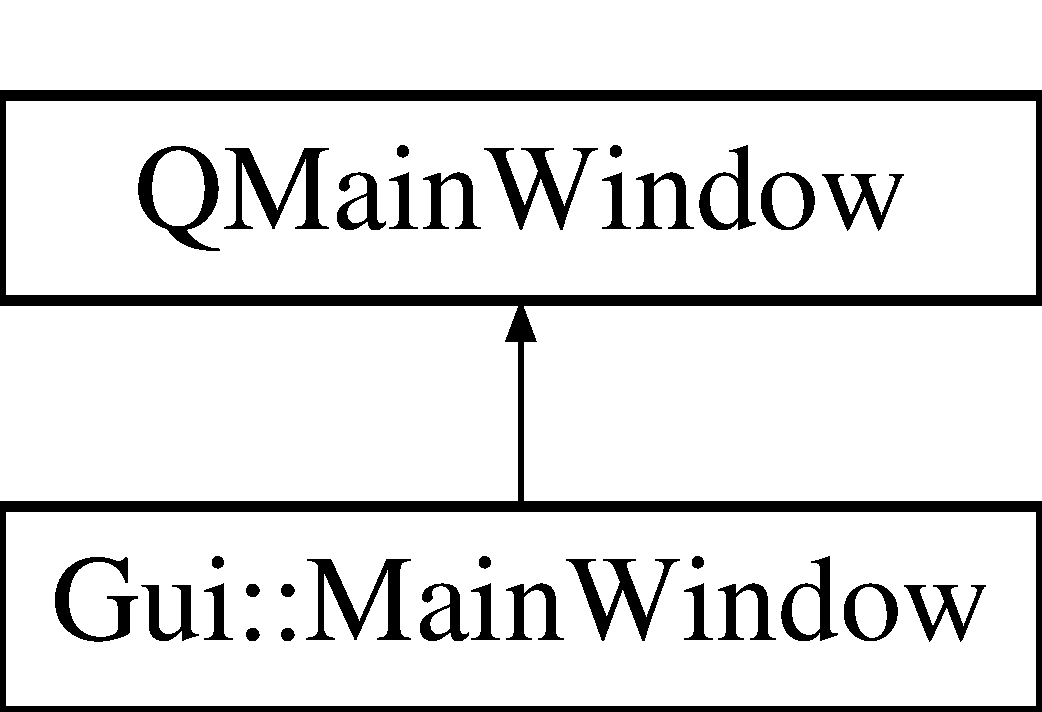
\includegraphics[height=2.000000cm]{d5/d2f/classGui_1_1MainWindow}
\end{center}
\end{figure}
\subsection*{Public Slots}
\begin{DoxyCompactItemize}
\item 
\hypertarget{classGui_1_1MainWindow_a52d033c14efb98b5b389121b8d60f2fe}{void \hyperlink{classGui_1_1MainWindow_a52d033c14efb98b5b389121b8d60f2fe}{add\-Customer} ()}\label{classGui_1_1MainWindow_a52d033c14efb98b5b389121b8d60f2fe}

\begin{DoxyCompactList}\small\item\em \hyperlink{classGui_1_1MainWindow_a52d033c14efb98b5b389121b8d60f2fe}{Main\-Window\-::add\-Customer} open window to add a new customer. \end{DoxyCompactList}\item 
\hypertarget{classGui_1_1MainWindow_a6487a725a2b58b89062944778ac59eca}{void \hyperlink{classGui_1_1MainWindow_a6487a725a2b58b89062944778ac59eca}{edit\-Customer} ()}\label{classGui_1_1MainWindow_a6487a725a2b58b89062944778ac59eca}

\begin{DoxyCompactList}\small\item\em \hyperlink{classGui_1_1MainWindow_a6487a725a2b58b89062944778ac59eca}{Main\-Window\-::edit\-Customer} open window to modify a customer. \end{DoxyCompactList}\item 
\hypertarget{classGui_1_1MainWindow_ab86dd052f06fb56dbd77e3ae4c228796}{void \hyperlink{classGui_1_1MainWindow_ab86dd052f06fb56dbd77e3ae4c228796}{remove\-Customer} ()}\label{classGui_1_1MainWindow_ab86dd052f06fb56dbd77e3ae4c228796}

\begin{DoxyCompactList}\small\item\em \hyperlink{classGui_1_1MainWindow_ab86dd052f06fb56dbd77e3ae4c228796}{Main\-Window\-::remove\-Customer} open a popup to confirm the deletion of a customer, if ok remove the customer. \end{DoxyCompactList}\item 
\hypertarget{classGui_1_1MainWindow_a8fb7964262a931657329a4c13afb2dad}{void \hyperlink{classGui_1_1MainWindow_a8fb7964262a931657329a4c13afb2dad}{archive\-Customer} ()}\label{classGui_1_1MainWindow_a8fb7964262a931657329a4c13afb2dad}

\begin{DoxyCompactList}\small\item\em \hyperlink{classGui_1_1MainWindow_a8fb7964262a931657329a4c13afb2dad}{Main\-Window\-::archive\-Customer} open a pop-\/up to confirm the archiving of the customer, if ok archive the customer. \end{DoxyCompactList}\item 
void \hyperlink{classGui_1_1MainWindow_aa7d3f2553b55d74885ad7f19ed403dfd}{add\-Quote} ()
\begin{DoxyCompactList}\small\item\em \hyperlink{classGui_1_1MainWindow_aa7d3f2553b55d74885ad7f19ed403dfd}{Main\-Window\-::add\-Quote} open window to add a new quote. \end{DoxyCompactList}\item 
void \hyperlink{classGui_1_1MainWindow_a4b9d5d9bee4b7a5f7d8cfe04d1222315}{add\-Bill} ()
\begin{DoxyCompactList}\small\item\em \hyperlink{classGui_1_1MainWindow_a4b9d5d9bee4b7a5f7d8cfe04d1222315}{Main\-Window\-::add\-Bill} open window to add a new bill. \end{DoxyCompactList}\item 
\hypertarget{classGui_1_1MainWindow_a149c8e2210fa249c0510e1f607079fde}{void \hyperlink{classGui_1_1MainWindow_a149c8e2210fa249c0510e1f607079fde}{billing\-Is\-Paid} ()}\label{classGui_1_1MainWindow_a149c8e2210fa249c0510e1f607079fde}

\begin{DoxyCompactList}\small\item\em \hyperlink{classGui_1_1MainWindow_a149c8e2210fa249c0510e1f607079fde}{Main\-Window\-::billing\-Is\-Paid} Define the current billing as \char`\"{}paid\char`\"{}. \end{DoxyCompactList}\item 
void \hyperlink{classGui_1_1MainWindow_a5dfb182cf52eb48f71e70cd193ef7a8b}{edit\-User} ()
\begin{DoxyCompactList}\small\item\em \hyperlink{classGui_1_1MainWindow_a5dfb182cf52eb48f71e70cd193ef7a8b}{Main\-Window\-::edit\-User} modify the user. \end{DoxyCompactList}\item 
void \hyperlink{classGui_1_1MainWindow_af50656b4c43aa53bae1ac4a3d6b4c953}{search} (Q\-String s)
\begin{DoxyCompactList}\small\item\em \hyperlink{classGui_1_1MainWindow_af50656b4c43aa53bae1ac4a3d6b4c953}{Main\-Window\-::search} launch a new search. \end{DoxyCompactList}\item 
void \hyperlink{classGui_1_1MainWindow_acc49a5a35dfc7eb8f835ff425618e2d9}{add\-Project} ()
\begin{DoxyCompactList}\small\item\em \hyperlink{classGui_1_1MainWindow_acc49a5a35dfc7eb8f835ff425618e2d9}{Main\-Window\-::add\-Project} Create a new project for a customer. \end{DoxyCompactList}\item 
\hypertarget{classGui_1_1MainWindow_aff6f88facb002c942273170d3543bb54}{void \hyperlink{classGui_1_1MainWindow_aff6f88facb002c942273170d3543bb54}{remove\-Project} ()}\label{classGui_1_1MainWindow_aff6f88facb002c942273170d3543bb54}

\begin{DoxyCompactList}\small\item\em \hyperlink{classGui_1_1MainWindow_aff6f88facb002c942273170d3543bb54}{Main\-Window\-::remove\-Project} Remove a project for a customer. \end{DoxyCompactList}\item 
\hypertarget{classGui_1_1MainWindow_a80af8e18d89a51a3368a65fb22e02040}{void \hyperlink{classGui_1_1MainWindow_a80af8e18d89a51a3368a65fb22e02040}{edit\-Project} ()}\label{classGui_1_1MainWindow_a80af8e18d89a51a3368a65fb22e02040}

\begin{DoxyCompactList}\small\item\em \hyperlink{classGui_1_1MainWindow_a80af8e18d89a51a3368a65fb22e02040}{Main\-Window\-::edit\-Project} Modify the customer project. \end{DoxyCompactList}\item 
\hypertarget{classGui_1_1MainWindow_a6df8072789ea8ec81ca2dd8fa78a4b01}{void \hyperlink{classGui_1_1MainWindow_a6df8072789ea8ec81ca2dd8fa78a4b01}{about\-Qt} ()}\label{classGui_1_1MainWindow_a6df8072789ea8ec81ca2dd8fa78a4b01}

\begin{DoxyCompactList}\small\item\em \hyperlink{classGui_1_1MainWindow_a6df8072789ea8ec81ca2dd8fa78a4b01}{Main\-Window\-::about\-Qt} show Qt's details. \end{DoxyCompactList}\item 
\hypertarget{classGui_1_1MainWindow_a26726203b873f41f607d78c5d5619c7d}{void \hyperlink{classGui_1_1MainWindow_a26726203b873f41f607d78c5d5619c7d}{about\-Fact} ()}\label{classGui_1_1MainWindow_a26726203b873f41f607d78c5d5619c7d}

\begin{DoxyCompactList}\small\item\em \hyperlink{classGui_1_1MainWindow_a26726203b873f41f607d78c5d5619c7d}{Main\-Window\-::about\-Fact} show F\-A\-C\-T's details (F\-A\-C\-T team) \end{DoxyCompactList}\item 
\hypertarget{classGui_1_1MainWindow_a39fe49fec47b6cbe4c8664d97bc47e0f}{void \hyperlink{classGui_1_1MainWindow_a39fe49fec47b6cbe4c8664d97bc47e0f}{about\-Fact\-Dev} ()}\label{classGui_1_1MainWindow_a39fe49fec47b6cbe4c8664d97bc47e0f}

\begin{DoxyCompactList}\small\item\em \hyperlink{classGui_1_1MainWindow_a39fe49fec47b6cbe4c8664d97bc47e0f}{Main\-Window\-::about\-Fact\-Dev()} show Fact\-Dev's details (Fact\-Dev Software) \end{DoxyCompactList}\item 
\hypertarget{classGui_1_1MainWindow_a56db09003bd79c8635488d0edc57cdb3}{void \hyperlink{classGui_1_1MainWindow_a56db09003bd79c8635488d0edc57cdb3}{about\-Icons} ()}\label{classGui_1_1MainWindow_a56db09003bd79c8635488d0edc57cdb3}

\begin{DoxyCompactList}\small\item\em \hyperlink{classGui_1_1MainWindow_a56db09003bd79c8635488d0edc57cdb3}{Main\-Window\-::about\-Icons()} show icons's details. \end{DoxyCompactList}\item 
\hypertarget{classGui_1_1MainWindow_aef4e1621cfa50a15b85921215c7171b8}{void \hyperlink{classGui_1_1MainWindow_aef4e1621cfa50a15b85921215c7171b8}{update\-Buttons} ()}\label{classGui_1_1MainWindow_aef4e1621cfa50a15b85921215c7171b8}

\begin{DoxyCompactList}\small\item\em update\-Button Update all button to disable or enabled its \end{DoxyCompactList}\item 
\hypertarget{classGui_1_1MainWindow_a06bc679c41574cb679c6e5e7b673139c}{void \hyperlink{classGui_1_1MainWindow_a06bc679c41574cb679c6e5e7b673139c}{edit\-Doc} ()}\label{classGui_1_1MainWindow_a06bc679c41574cb679c6e5e7b673139c}

\begin{DoxyCompactList}\small\item\em \hyperlink{classGui_1_1MainWindow_a06bc679c41574cb679c6e5e7b673139c}{Main\-Window\-::edit\-Doc} Edit the quote or bill of the project. \end{DoxyCompactList}\item 
\hypertarget{classGui_1_1MainWindow_af86458ad953cb70fb7a88245a6047550}{void \hyperlink{classGui_1_1MainWindow_af86458ad953cb70fb7a88245a6047550}{remove\-Doc} ()}\label{classGui_1_1MainWindow_af86458ad953cb70fb7a88245a6047550}

\begin{DoxyCompactList}\small\item\em \hyperlink{classGui_1_1MainWindow_af86458ad953cb70fb7a88245a6047550}{Main\-Window\-::remove\-Doc} Remove the quote or bill of the project. \end{DoxyCompactList}\item 
\hypertarget{classGui_1_1MainWindow_adf1e721c73626d1810dd90c84920dcde}{void \hyperlink{classGui_1_1MainWindow_adf1e721c73626d1810dd90c84920dcde}{copy\-Doc} ()}\label{classGui_1_1MainWindow_adf1e721c73626d1810dd90c84920dcde}

\begin{DoxyCompactList}\small\item\em \hyperlink{classGui_1_1MainWindow_adf1e721c73626d1810dd90c84920dcde}{Main\-Window\-::copy\-Doc} Copy all elements of a quote or a bill and Display these elements in a new quote or bill. \end{DoxyCompactList}\item 
\hypertarget{classGui_1_1MainWindow_a6fc6c0f088d3996ad941705a13d7aaae}{void \hyperlink{classGui_1_1MainWindow_a6fc6c0f088d3996ad941705a13d7aaae}{open\-Pdf} ()}\label{classGui_1_1MainWindow_a6fc6c0f088d3996ad941705a13d7aaae}

\begin{DoxyCompactList}\small\item\em \hyperlink{classGui_1_1MainWindow_a6fc6c0f088d3996ad941705a13d7aaae}{Main\-Window\-::open\-Pdf} Open the P\-D\-F file of the current Quote or Billing selected in the Table\-View. \end{DoxyCompactList}\item 
\hypertarget{classGui_1_1MainWindow_aa4cfc2b980835fe1ccd5b869a237c05f}{void \hyperlink{classGui_1_1MainWindow_aa4cfc2b980835fe1ccd5b869a237c05f}{compute\-Turnover} ()}\label{classGui_1_1MainWindow_aa4cfc2b980835fe1ccd5b869a237c05f}

\begin{DoxyCompactList}\small\item\em \hyperlink{classGui_1_1MainWindow_aa4cfc2b980835fe1ccd5b869a237c05f}{Main\-Window\-::compute\-Turnover} open window to allow computation of a period turnover. \end{DoxyCompactList}\item 
\hypertarget{classGui_1_1MainWindow_a41e44415a270150b6630efcb87768d7f}{void \hyperlink{classGui_1_1MainWindow_a41e44415a270150b6630efcb87768d7f}{global\-Statistics} ()}\label{classGui_1_1MainWindow_a41e44415a270150b6630efcb87768d7f}

\begin{DoxyCompactList}\small\item\em \hyperlink{classGui_1_1MainWindow_a41e44415a270150b6630efcb87768d7f}{Main\-Window\-::global\-Statistics}. \end{DoxyCompactList}\item 
\hypertarget{classGui_1_1MainWindow_a078b2546e65d2b91d3b2b546db619adb}{void \hyperlink{classGui_1_1MainWindow_a078b2546e65d2b91d3b2b546db619adb}{customer\-Statistics} ()}\label{classGui_1_1MainWindow_a078b2546e65d2b91d3b2b546db619adb}

\begin{DoxyCompactList}\small\item\em \hyperlink{classGui_1_1MainWindow_a078b2546e65d2b91d3b2b546db619adb}{Main\-Window\-::customer\-Statistics}. \end{DoxyCompactList}\item 
\hypertarget{classGui_1_1MainWindow_a96335036187601e48bb46945d57fc2a5}{void \hyperlink{classGui_1_1MainWindow_a96335036187601e48bb46945d57fc2a5}{lock\-Project} ()}\label{classGui_1_1MainWindow_a96335036187601e48bb46945d57fc2a5}

\begin{DoxyCompactList}\small\item\em lock\-Project Lock the current project \end{DoxyCompactList}\item 
\hypertarget{classGui_1_1MainWindow_adc45883c353219dcfbb15a3bc356909a}{void {\bfseries merge\-Docks} ()}\label{classGui_1_1MainWindow_adc45883c353219dcfbb15a3bc356909a}

\end{DoxyCompactItemize}
\subsection*{Public Member Functions}
\begin{DoxyCompactItemize}
\item 
\hyperlink{classGui_1_1MainWindow_a5ea8e526d288b96595618942d44154d3}{Main\-Window} (Q\-Widget $\ast$parent=0)
\begin{DoxyCompactList}\small\item\em \hyperlink{classGui_1_1MainWindow}{Main\-Window}\-: Construct a window. \end{DoxyCompactList}\item 
int \hyperlink{classGui_1_1MainWindow_a202cb1e7a7c0e47af15306c2587693ec}{get\-Current\-Customer\-Id} ()
\begin{DoxyCompactList}\small\item\em \hyperlink{classGui_1_1MainWindow_a202cb1e7a7c0e47af15306c2587693ec}{Main\-Window\-::get\-Current\-Customer\-Id} get the selected customer. \end{DoxyCompactList}\item 
int \hyperlink{classGui_1_1MainWindow_a9580e96fd90710c5e2c299c68108409a}{get\-Current\-Project\-Id} ()
\begin{DoxyCompactList}\small\item\em \hyperlink{classGui_1_1MainWindow_a9580e96fd90710c5e2c299c68108409a}{Main\-Window\-::get\-Current\-Project\-Id} get the selected project id. \end{DoxyCompactList}\item 
int \hyperlink{classGui_1_1MainWindow_aaf5e1b2cb797894207f4c5e86d2d4dcf}{get\-Current\-Quote\-Id} ()
\begin{DoxyCompactList}\small\item\em \hyperlink{classGui_1_1MainWindow_aaf5e1b2cb797894207f4c5e86d2d4dcf}{Main\-Window\-::get\-Current\-Quote\-Id} get the selected quote id. \end{DoxyCompactList}\item 
Q\-String \hyperlink{classGui_1_1MainWindow_a0303a1752424b1e8c1a6e1b0bba2a823}{get\-Current\-Customer\-Name} ()
\begin{DoxyCompactList}\small\item\em \hyperlink{classGui_1_1MainWindow_a0303a1752424b1e8c1a6e1b0bba2a823}{Main\-Window\-::get\-Current\-Customer\-Name} get the selected customer name in the customers' table. \end{DoxyCompactList}\item 
Q\-String \hyperlink{classGui_1_1MainWindow_af83b009038b41bc676d15cb9bcfd5a39}{get\-Current\-Project\-Name} ()
\begin{DoxyCompactList}\small\item\em \hyperlink{classGui_1_1MainWindow_af83b009038b41bc676d15cb9bcfd5a39}{Main\-Window\-::get\-Current\-Project\-Name} get the selected project name in the table of projects. \end{DoxyCompactList}\item 
int \hyperlink{classGui_1_1MainWindow_a382370c8f119d99d409b1b5708a3e846}{tree\-Level} ()
\begin{DoxyCompactList}\small\item\em \hyperlink{classGui_1_1MainWindow_a382370c8f119d99d409b1b5708a3e846}{Main\-Window\-::tree\-Level} return the level of the node selected in the tree. \end{DoxyCompactList}\item 
Q\-Model\-Index \hyperlink{classGui_1_1MainWindow_ad2b58d18473d125b431ee0974c905748}{root\-Tree} ()
\begin{DoxyCompactList}\small\item\em \hyperlink{classGui_1_1MainWindow_ad2b58d18473d125b431ee0974c905748}{Main\-Window\-::root\-Tree} return the root of the tree \char`\"{}\-Tous les
clients\char`\"{}. \end{DoxyCompactList}\item 
void \hyperlink{classGui_1_1MainWindow_adf04c63032d4014163797ca73041511f}{add\-Doc} (bool is\-Billing)
\begin{DoxyCompactList}\small\item\em \hyperlink{classGui_1_1MainWindow_adf04c63032d4014163797ca73041511f}{Main\-Window\-::add\-Doc} open window to add a new document. \end{DoxyCompactList}\item 
void \hyperlink{classGui_1_1MainWindow_a7c85d2a0d68c046fa678bdc12feef96d}{resize\-Event} (Q\-Resize\-Event $\ast$event)
\begin{DoxyCompactList}\small\item\em \hyperlink{classGui_1_1MainWindow_a7c85d2a0d68c046fa678bdc12feef96d}{Main\-Window\-::resize\-Event} Resize central Table\-View when you resize the {\bfseries \hyperlink{classGui_1_1MainWindow}{Main\-Window}} \end{DoxyCompactList}\item 
\hypertarget{classGui_1_1MainWindow_a0bf829effb9cb3e42ba063335a15cf3d}{void \hyperlink{classGui_1_1MainWindow_a0bf829effb9cb3e42ba063335a15cf3d}{responsive\-Customer\-Table} ()}\label{classGui_1_1MainWindow_a0bf829effb9cb3e42ba063335a15cf3d}

\begin{DoxyCompactList}\small\item\em \hyperlink{classGui_1_1MainWindow_a0bf829effb9cb3e42ba063335a15cf3d}{Main\-Window\-::responsive\-Customer\-Table} Resize the Customer Table\-View according it resolution. \end{DoxyCompactList}\item 
\hypertarget{classGui_1_1MainWindow_af7402e6aa57ddf139ba82fb49c497cab}{void \hyperlink{classGui_1_1MainWindow_af7402e6aa57ddf139ba82fb49c497cab}{responsive\-Project\-Table} ()}\label{classGui_1_1MainWindow_af7402e6aa57ddf139ba82fb49c497cab}

\begin{DoxyCompactList}\small\item\em \hyperlink{classGui_1_1MainWindow_af7402e6aa57ddf139ba82fb49c497cab}{Main\-Window\-::responsive\-Project\-Table} Resize the Project Table\-View according it resolution. \end{DoxyCompactList}\item 
\hypertarget{classGui_1_1MainWindow_aff185fab5a7499468d8523d4db1592c9}{void \hyperlink{classGui_1_1MainWindow_aff185fab5a7499468d8523d4db1592c9}{responsive\-Billing\-Table} ()}\label{classGui_1_1MainWindow_aff185fab5a7499468d8523d4db1592c9}

\begin{DoxyCompactList}\small\item\em \hyperlink{classGui_1_1MainWindow_aff185fab5a7499468d8523d4db1592c9}{Main\-Window\-::responsive\-Billing\-Table} Resize the Billing Table\-View according it resolution. \end{DoxyCompactList}\item 
bool \hyperlink{classGui_1_1MainWindow_a2cacb5b7aa0109215473a6e59d28151c}{is\-Easter\-Egg} (const Q\-String filter)
\begin{DoxyCompactList}\small\item\em \hyperlink{classGui_1_1MainWindow_a2cacb5b7aa0109215473a6e59d28151c}{Main\-Window\-::is\-Easter\-Egg} Return T\-R\-U\-E if search {\itshape filter} is {\bfseries Fleury\-Migeon42} else F\-A\-L\-S\-E. \end{DoxyCompactList}\end{DoxyCompactItemize}


\subsection{Detailed Description}
The \hyperlink{classGui_1_1MainWindow}{Main\-Window} class Main Window of the software. 

\begin{DoxyAuthor}{Author}
Everybody 
\end{DoxyAuthor}


\subsection{Constructor \& Destructor Documentation}
\hypertarget{classGui_1_1MainWindow_a5ea8e526d288b96595618942d44154d3}{\index{Gui\-::\-Main\-Window@{Gui\-::\-Main\-Window}!Main\-Window@{Main\-Window}}
\index{Main\-Window@{Main\-Window}!Gui::MainWindow@{Gui\-::\-Main\-Window}}
\subsubsection[{Main\-Window}]{\setlength{\rightskip}{0pt plus 5cm}Gui\-::\-Main\-Window\-::\-Main\-Window (
\begin{DoxyParamCaption}
\item[{Q\-Widget $\ast$}]{parent = {\ttfamily 0}}
\end{DoxyParamCaption}
)\hspace{0.3cm}{\ttfamily [explicit]}}}\label{classGui_1_1MainWindow_a5ea8e526d288b96595618942d44154d3}


\hyperlink{classGui_1_1MainWindow}{Main\-Window}\-: Construct a window. 


\begin{DoxyParams}{Parameters}
{\em parent} & \\
\hline
\end{DoxyParams}


\subsection{Member Function Documentation}
\hypertarget{classGui_1_1MainWindow_a4b9d5d9bee4b7a5f7d8cfe04d1222315}{\index{Gui\-::\-Main\-Window@{Gui\-::\-Main\-Window}!add\-Bill@{add\-Bill}}
\index{add\-Bill@{add\-Bill}!Gui::MainWindow@{Gui\-::\-Main\-Window}}
\subsubsection[{add\-Bill}]{\setlength{\rightskip}{0pt plus 5cm}void Gui\-::\-Main\-Window\-::add\-Bill (
\begin{DoxyParamCaption}
{}
\end{DoxyParamCaption}
)\hspace{0.3cm}{\ttfamily [slot]}}}\label{classGui_1_1MainWindow_a4b9d5d9bee4b7a5f7d8cfe04d1222315}


\hyperlink{classGui_1_1MainWindow_a4b9d5d9bee4b7a5f7d8cfe04d1222315}{Main\-Window\-::add\-Bill} open window to add a new bill. 

\begin{DoxySeeAlso}{See Also}
Add\-Quote\-Dialog 
\end{DoxySeeAlso}
\hypertarget{classGui_1_1MainWindow_adf04c63032d4014163797ca73041511f}{\index{Gui\-::\-Main\-Window@{Gui\-::\-Main\-Window}!add\-Doc@{add\-Doc}}
\index{add\-Doc@{add\-Doc}!Gui::MainWindow@{Gui\-::\-Main\-Window}}
\subsubsection[{add\-Doc}]{\setlength{\rightskip}{0pt plus 5cm}void Gui\-::\-Main\-Window\-::add\-Doc (
\begin{DoxyParamCaption}
\item[{bool}]{is\-Billing}
\end{DoxyParamCaption}
)}}\label{classGui_1_1MainWindow_adf04c63032d4014163797ca73041511f}


\hyperlink{classGui_1_1MainWindow_adf04c63032d4014163797ca73041511f}{Main\-Window\-::add\-Doc} open window to add a new document. 


\begin{DoxyParams}{Parameters}
{\em bool} & quote or bill \\
\hline
\end{DoxyParams}
\begin{DoxySeeAlso}{See Also}
\hyperlink{classGui_1_1MainWindow_a4b9d5d9bee4b7a5f7d8cfe04d1222315}{add\-Bill} \hyperlink{classGui_1_1MainWindow_aa7d3f2553b55d74885ad7f19ed403dfd}{add\-Quote} 
\end{DoxySeeAlso}
\hypertarget{classGui_1_1MainWindow_acc49a5a35dfc7eb8f835ff425618e2d9}{\index{Gui\-::\-Main\-Window@{Gui\-::\-Main\-Window}!add\-Project@{add\-Project}}
\index{add\-Project@{add\-Project}!Gui::MainWindow@{Gui\-::\-Main\-Window}}
\subsubsection[{add\-Project}]{\setlength{\rightskip}{0pt plus 5cm}void Gui\-::\-Main\-Window\-::add\-Project (
\begin{DoxyParamCaption}
{}
\end{DoxyParamCaption}
)\hspace{0.3cm}{\ttfamily [slot]}}}\label{classGui_1_1MainWindow_acc49a5a35dfc7eb8f835ff425618e2d9}


\hyperlink{classGui_1_1MainWindow_acc49a5a35dfc7eb8f835ff425618e2d9}{Main\-Window\-::add\-Project} Create a new project for a customer. 

\begin{DoxySeeAlso}{See Also}
Add\-Project\-Dialog 
\end{DoxySeeAlso}
\hypertarget{classGui_1_1MainWindow_aa7d3f2553b55d74885ad7f19ed403dfd}{\index{Gui\-::\-Main\-Window@{Gui\-::\-Main\-Window}!add\-Quote@{add\-Quote}}
\index{add\-Quote@{add\-Quote}!Gui::MainWindow@{Gui\-::\-Main\-Window}}
\subsubsection[{add\-Quote}]{\setlength{\rightskip}{0pt plus 5cm}void Gui\-::\-Main\-Window\-::add\-Quote (
\begin{DoxyParamCaption}
{}
\end{DoxyParamCaption}
)\hspace{0.3cm}{\ttfamily [slot]}}}\label{classGui_1_1MainWindow_aa7d3f2553b55d74885ad7f19ed403dfd}


\hyperlink{classGui_1_1MainWindow_aa7d3f2553b55d74885ad7f19ed403dfd}{Main\-Window\-::add\-Quote} open window to add a new quote. 

\begin{DoxySeeAlso}{See Also}
Add\-Quote\-Dialog 
\end{DoxySeeAlso}
\hypertarget{classGui_1_1MainWindow_a5dfb182cf52eb48f71e70cd193ef7a8b}{\index{Gui\-::\-Main\-Window@{Gui\-::\-Main\-Window}!edit\-User@{edit\-User}}
\index{edit\-User@{edit\-User}!Gui::MainWindow@{Gui\-::\-Main\-Window}}
\subsubsection[{edit\-User}]{\setlength{\rightskip}{0pt plus 5cm}void Gui\-::\-Main\-Window\-::edit\-User (
\begin{DoxyParamCaption}
{}
\end{DoxyParamCaption}
)\hspace{0.3cm}{\ttfamily [slot]}}}\label{classGui_1_1MainWindow_a5dfb182cf52eb48f71e70cd193ef7a8b}


\hyperlink{classGui_1_1MainWindow_a5dfb182cf52eb48f71e70cd193ef7a8b}{Main\-Window\-::edit\-User} modify the user. 

\begin{DoxySeeAlso}{See Also}
User\-Data\-Dialog 
\end{DoxySeeAlso}
\hypertarget{classGui_1_1MainWindow_a202cb1e7a7c0e47af15306c2587693ec}{\index{Gui\-::\-Main\-Window@{Gui\-::\-Main\-Window}!get\-Current\-Customer\-Id@{get\-Current\-Customer\-Id}}
\index{get\-Current\-Customer\-Id@{get\-Current\-Customer\-Id}!Gui::MainWindow@{Gui\-::\-Main\-Window}}
\subsubsection[{get\-Current\-Customer\-Id}]{\setlength{\rightskip}{0pt plus 5cm}int Gui\-::\-Main\-Window\-::get\-Current\-Customer\-Id (
\begin{DoxyParamCaption}
{}
\end{DoxyParamCaption}
)}}\label{classGui_1_1MainWindow_a202cb1e7a7c0e47af15306c2587693ec}


\hyperlink{classGui_1_1MainWindow_a202cb1e7a7c0e47af15306c2587693ec}{Main\-Window\-::get\-Current\-Customer\-Id} get the selected customer. 

\begin{DoxyReturn}{Returns}
id of the selected customer 
\end{DoxyReturn}
\hypertarget{classGui_1_1MainWindow_a0303a1752424b1e8c1a6e1b0bba2a823}{\index{Gui\-::\-Main\-Window@{Gui\-::\-Main\-Window}!get\-Current\-Customer\-Name@{get\-Current\-Customer\-Name}}
\index{get\-Current\-Customer\-Name@{get\-Current\-Customer\-Name}!Gui::MainWindow@{Gui\-::\-Main\-Window}}
\subsubsection[{get\-Current\-Customer\-Name}]{\setlength{\rightskip}{0pt plus 5cm}Q\-String Gui\-::\-Main\-Window\-::get\-Current\-Customer\-Name (
\begin{DoxyParamCaption}
{}
\end{DoxyParamCaption}
)}}\label{classGui_1_1MainWindow_a0303a1752424b1e8c1a6e1b0bba2a823}


\hyperlink{classGui_1_1MainWindow_a0303a1752424b1e8c1a6e1b0bba2a823}{Main\-Window\-::get\-Current\-Customer\-Name} get the selected customer name in the customers' table. 

\begin{DoxyReturn}{Returns}
name of the selected customer 
\end{DoxyReturn}
\hypertarget{classGui_1_1MainWindow_a9580e96fd90710c5e2c299c68108409a}{\index{Gui\-::\-Main\-Window@{Gui\-::\-Main\-Window}!get\-Current\-Project\-Id@{get\-Current\-Project\-Id}}
\index{get\-Current\-Project\-Id@{get\-Current\-Project\-Id}!Gui::MainWindow@{Gui\-::\-Main\-Window}}
\subsubsection[{get\-Current\-Project\-Id}]{\setlength{\rightskip}{0pt plus 5cm}int Gui\-::\-Main\-Window\-::get\-Current\-Project\-Id (
\begin{DoxyParamCaption}
{}
\end{DoxyParamCaption}
)}}\label{classGui_1_1MainWindow_a9580e96fd90710c5e2c299c68108409a}


\hyperlink{classGui_1_1MainWindow_a9580e96fd90710c5e2c299c68108409a}{Main\-Window\-::get\-Current\-Project\-Id} get the selected project id. 

\begin{DoxyReturn}{Returns}
id of the selected project 
\end{DoxyReturn}
\hypertarget{classGui_1_1MainWindow_af83b009038b41bc676d15cb9bcfd5a39}{\index{Gui\-::\-Main\-Window@{Gui\-::\-Main\-Window}!get\-Current\-Project\-Name@{get\-Current\-Project\-Name}}
\index{get\-Current\-Project\-Name@{get\-Current\-Project\-Name}!Gui::MainWindow@{Gui\-::\-Main\-Window}}
\subsubsection[{get\-Current\-Project\-Name}]{\setlength{\rightskip}{0pt plus 5cm}Q\-String Gui\-::\-Main\-Window\-::get\-Current\-Project\-Name (
\begin{DoxyParamCaption}
{}
\end{DoxyParamCaption}
)}}\label{classGui_1_1MainWindow_af83b009038b41bc676d15cb9bcfd5a39}


\hyperlink{classGui_1_1MainWindow_af83b009038b41bc676d15cb9bcfd5a39}{Main\-Window\-::get\-Current\-Project\-Name} get the selected project name in the table of projects. 

\begin{DoxyReturn}{Returns}
name of the selected project 
\end{DoxyReturn}
\hypertarget{classGui_1_1MainWindow_aaf5e1b2cb797894207f4c5e86d2d4dcf}{\index{Gui\-::\-Main\-Window@{Gui\-::\-Main\-Window}!get\-Current\-Quote\-Id@{get\-Current\-Quote\-Id}}
\index{get\-Current\-Quote\-Id@{get\-Current\-Quote\-Id}!Gui::MainWindow@{Gui\-::\-Main\-Window}}
\subsubsection[{get\-Current\-Quote\-Id}]{\setlength{\rightskip}{0pt plus 5cm}int Gui\-::\-Main\-Window\-::get\-Current\-Quote\-Id (
\begin{DoxyParamCaption}
{}
\end{DoxyParamCaption}
)}}\label{classGui_1_1MainWindow_aaf5e1b2cb797894207f4c5e86d2d4dcf}


\hyperlink{classGui_1_1MainWindow_aaf5e1b2cb797894207f4c5e86d2d4dcf}{Main\-Window\-::get\-Current\-Quote\-Id} get the selected quote id. 

\begin{DoxyReturn}{Returns}
id of the selected quote 
\end{DoxyReturn}
\hypertarget{classGui_1_1MainWindow_a2cacb5b7aa0109215473a6e59d28151c}{\index{Gui\-::\-Main\-Window@{Gui\-::\-Main\-Window}!is\-Easter\-Egg@{is\-Easter\-Egg}}
\index{is\-Easter\-Egg@{is\-Easter\-Egg}!Gui::MainWindow@{Gui\-::\-Main\-Window}}
\subsubsection[{is\-Easter\-Egg}]{\setlength{\rightskip}{0pt plus 5cm}bool Gui\-::\-Main\-Window\-::is\-Easter\-Egg (
\begin{DoxyParamCaption}
\item[{const Q\-String}]{filter}
\end{DoxyParamCaption}
)}}\label{classGui_1_1MainWindow_a2cacb5b7aa0109215473a6e59d28151c}


\hyperlink{classGui_1_1MainWindow_a2cacb5b7aa0109215473a6e59d28151c}{Main\-Window\-::is\-Easter\-Egg} Return T\-R\-U\-E if search {\itshape filter} is {\bfseries Fleury\-Migeon42} else F\-A\-L\-S\-E. 


\begin{DoxyParams}{Parameters}
{\em filter} & Search filter \\
\hline
\end{DoxyParams}
\begin{DoxyReturn}{Returns}
boolean 
\end{DoxyReturn}
\hypertarget{classGui_1_1MainWindow_a7c85d2a0d68c046fa678bdc12feef96d}{\index{Gui\-::\-Main\-Window@{Gui\-::\-Main\-Window}!resize\-Event@{resize\-Event}}
\index{resize\-Event@{resize\-Event}!Gui::MainWindow@{Gui\-::\-Main\-Window}}
\subsubsection[{resize\-Event}]{\setlength{\rightskip}{0pt plus 5cm}void Gui\-::\-Main\-Window\-::resize\-Event (
\begin{DoxyParamCaption}
\item[{Q\-Resize\-Event $\ast$}]{event}
\end{DoxyParamCaption}
)}}\label{classGui_1_1MainWindow_a7c85d2a0d68c046fa678bdc12feef96d}


\hyperlink{classGui_1_1MainWindow_a7c85d2a0d68c046fa678bdc12feef96d}{Main\-Window\-::resize\-Event} Resize central Table\-View when you resize the {\bfseries \hyperlink{classGui_1_1MainWindow}{Main\-Window}} 


\begin{DoxyParams}{Parameters}
{\em event} & Resize event \\
\hline
\end{DoxyParams}
\hypertarget{classGui_1_1MainWindow_ad2b58d18473d125b431ee0974c905748}{\index{Gui\-::\-Main\-Window@{Gui\-::\-Main\-Window}!root\-Tree@{root\-Tree}}
\index{root\-Tree@{root\-Tree}!Gui::MainWindow@{Gui\-::\-Main\-Window}}
\subsubsection[{root\-Tree}]{\setlength{\rightskip}{0pt plus 5cm}Q\-Model\-Index Gui\-::\-Main\-Window\-::root\-Tree (
\begin{DoxyParamCaption}
{}
\end{DoxyParamCaption}
)}}\label{classGui_1_1MainWindow_ad2b58d18473d125b431ee0974c905748}


\hyperlink{classGui_1_1MainWindow_ad2b58d18473d125b431ee0974c905748}{Main\-Window\-::root\-Tree} return the root of the tree \char`\"{}\-Tous les
clients\char`\"{}. 

\begin{DoxyReturn}{Returns}
Q\-Model\-Index 
\end{DoxyReturn}
\hypertarget{classGui_1_1MainWindow_af50656b4c43aa53bae1ac4a3d6b4c953}{\index{Gui\-::\-Main\-Window@{Gui\-::\-Main\-Window}!search@{search}}
\index{search@{search}!Gui::MainWindow@{Gui\-::\-Main\-Window}}
\subsubsection[{search}]{\setlength{\rightskip}{0pt plus 5cm}void Gui\-::\-Main\-Window\-::search (
\begin{DoxyParamCaption}
\item[{Q\-String}]{s}
\end{DoxyParamCaption}
)\hspace{0.3cm}{\ttfamily [slot]}}}\label{classGui_1_1MainWindow_af50656b4c43aa53bae1ac4a3d6b4c953}


\hyperlink{classGui_1_1MainWindow_af50656b4c43aa53bae1ac4a3d6b4c953}{Main\-Window\-::search} launch a new search. 


\begin{DoxyParams}{Parameters}
{\em s} & text in field \\
\hline
\end{DoxyParams}
\hypertarget{classGui_1_1MainWindow_a382370c8f119d99d409b1b5708a3e846}{\index{Gui\-::\-Main\-Window@{Gui\-::\-Main\-Window}!tree\-Level@{tree\-Level}}
\index{tree\-Level@{tree\-Level}!Gui::MainWindow@{Gui\-::\-Main\-Window}}
\subsubsection[{tree\-Level}]{\setlength{\rightskip}{0pt plus 5cm}int Gui\-::\-Main\-Window\-::tree\-Level (
\begin{DoxyParamCaption}
{}
\end{DoxyParamCaption}
)}}\label{classGui_1_1MainWindow_a382370c8f119d99d409b1b5708a3e846}


\hyperlink{classGui_1_1MainWindow_a382370c8f119d99d409b1b5708a3e846}{Main\-Window\-::tree\-Level} return the level of the node selected in the tree. 

\begin{DoxyReturn}{Returns}
integer, depth of the item in tree 
\end{DoxyReturn}


The documentation for this class was generated from the following files\-:\begin{DoxyCompactItemize}
\item 
/home/travis/build/\-F\-A\-C\-T-\/\-Team/\-Fact\-Dev/src/gui/mainwindow/mainwindow.\-h\item 
/home/travis/build/\-F\-A\-C\-T-\/\-Team/\-Fact\-Dev/src/gui/mainwindow/mainwindow.\-cpp\end{DoxyCompactItemize}

\hypertarget{classGui_1_1Dialogs_1_1MessageBox}{\section{Gui\-:\-:Dialogs\-:\-:Message\-Box Class Reference}
\label{classGui_1_1Dialogs_1_1MessageBox}\index{Gui\-::\-Dialogs\-::\-Message\-Box@{Gui\-::\-Dialogs\-::\-Message\-Box}}
}


The \hyperlink{classGui_1_1Dialogs_1_1MessageBox}{Message\-Box} class Information window with message.  




{\ttfamily \#include $<$messagebox.\-h$>$}

Inheritance diagram for Gui\-:\-:Dialogs\-:\-:Message\-Box\-:\begin{figure}[H]
\begin{center}
\leavevmode
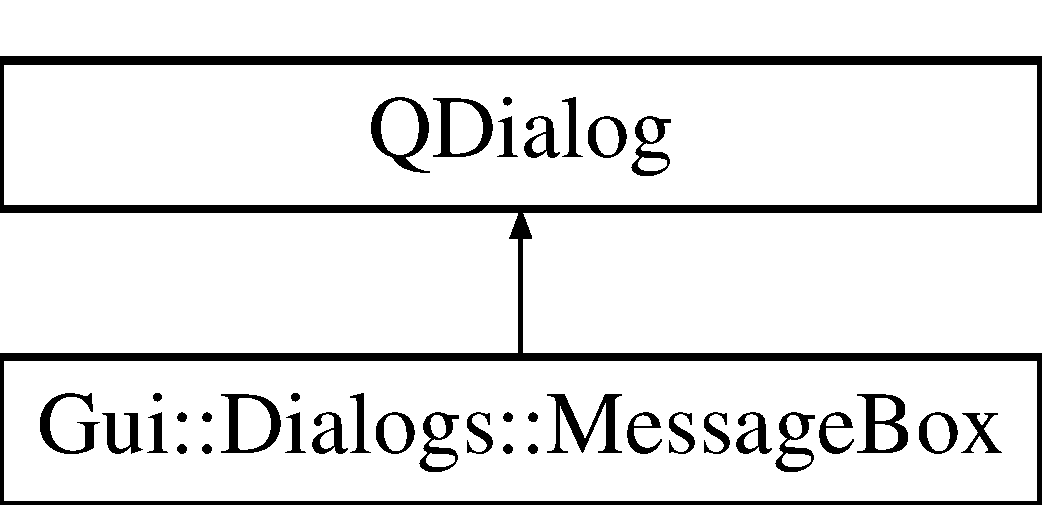
\includegraphics[height=2.000000cm]{d9/d31/classGui_1_1Dialogs_1_1MessageBox}
\end{center}
\end{figure}
\subsection*{Public Member Functions}
\begin{DoxyCompactItemize}
\item 
\hyperlink{classGui_1_1Dialogs_1_1MessageBox_ad5f6041f0f540c6d32b9feb7f139fa53}{Message\-Box} (Q\-Widget $\ast$parent=0)
\begin{DoxyCompactList}\small\item\em \hyperlink{classGui_1_1Dialogs_1_1MessageBox_ad5f6041f0f540c6d32b9feb7f139fa53}{Message\-Box\-::\-Message\-Box} Construt a {\bfseries \hyperlink{classGui_1_1Dialogs_1_1MessageBox}{Message\-Box}} \end{DoxyCompactList}\item 
\hypertarget{classGui_1_1Dialogs_1_1MessageBox_acda77dd0e2edd3aa85b1de11ed7899a2}{void \hyperlink{classGui_1_1Dialogs_1_1MessageBox_acda77dd0e2edd3aa85b1de11ed7899a2}{about\-Fact} ()}\label{classGui_1_1Dialogs_1_1MessageBox_acda77dd0e2edd3aa85b1de11ed7899a2}

\begin{DoxyCompactList}\small\item\em \hyperlink{classGui_1_1Dialogs_1_1MessageBox_acda77dd0e2edd3aa85b1de11ed7899a2}{Message\-Box\-::about\-Fact} Defines F\-A\-C\-T team information. \end{DoxyCompactList}\item 
\hypertarget{classGui_1_1Dialogs_1_1MessageBox_a0b92573a4e1ff4d44e8259d86b5b8275}{void \hyperlink{classGui_1_1Dialogs_1_1MessageBox_a0b92573a4e1ff4d44e8259d86b5b8275}{about\-Fact\-Dev} ()}\label{classGui_1_1Dialogs_1_1MessageBox_a0b92573a4e1ff4d44e8259d86b5b8275}

\begin{DoxyCompactList}\small\item\em \hyperlink{classGui_1_1Dialogs_1_1MessageBox_a0b92573a4e1ff4d44e8259d86b5b8275}{Message\-Box\-::about\-Fact\-Dev} Defines Fact\-Dev software information. \end{DoxyCompactList}\item 
\hypertarget{classGui_1_1Dialogs_1_1MessageBox_a196094a26db9cff58e70801186b73453}{void \hyperlink{classGui_1_1Dialogs_1_1MessageBox_a196094a26db9cff58e70801186b73453}{about\-Icons} ()}\label{classGui_1_1Dialogs_1_1MessageBox_a196094a26db9cff58e70801186b73453}

\begin{DoxyCompactList}\small\item\em \hyperlink{classGui_1_1Dialogs_1_1MessageBox_a196094a26db9cff58e70801186b73453}{Message\-Box\-::about\-Icons} Defines icons theme information. \end{DoxyCompactList}\item 
void \hyperlink{classGui_1_1Dialogs_1_1MessageBox_a4efd7f861c6338389dc7f42993413009}{set\-Image} (Q\-String img, int width=128, int height=128)
\begin{DoxyCompactList}\small\item\em \hyperlink{classGui_1_1Dialogs_1_1MessageBox_a4efd7f861c6338389dc7f42993413009}{Message\-Box\-::set\-Image} Add the icon {\itshape img} to the current window. \end{DoxyCompactList}\item 
void \hyperlink{classGui_1_1Dialogs_1_1MessageBox_af96c089b5fecffac59f2a337bad533cf}{set\-Text} (Q\-String txt)
\begin{DoxyCompactList}\small\item\em \hyperlink{classGui_1_1Dialogs_1_1MessageBox_af96c089b5fecffac59f2a337bad533cf}{Message\-Box\-::set\-Text} Add the text {\itshape txt} to the current window. \end{DoxyCompactList}\end{DoxyCompactItemize}
\subsection*{Static Public Member Functions}
\begin{DoxyCompactItemize}
\item 
\hypertarget{classGui_1_1Dialogs_1_1MessageBox_ad00c9885477fb131a87e75abc9b88fb4}{static void \hyperlink{classGui_1_1Dialogs_1_1MessageBox_ad00c9885477fb131a87e75abc9b88fb4}{show\-About\-Fact} ()}\label{classGui_1_1Dialogs_1_1MessageBox_ad00c9885477fb131a87e75abc9b88fb4}

\begin{DoxyCompactList}\small\item\em \hyperlink{classGui_1_1Dialogs_1_1MessageBox_ad00c9885477fb131a87e75abc9b88fb4}{Message\-Box\-::show\-About\-Fact} Shows window about F\-A\-C\-T team. \end{DoxyCompactList}\item 
\hypertarget{classGui_1_1Dialogs_1_1MessageBox_a5d17e7db09f46eb20fce54135b850497}{static void \hyperlink{classGui_1_1Dialogs_1_1MessageBox_a5d17e7db09f46eb20fce54135b850497}{show\-About\-Fact\-Dev} ()}\label{classGui_1_1Dialogs_1_1MessageBox_a5d17e7db09f46eb20fce54135b850497}

\begin{DoxyCompactList}\small\item\em \hyperlink{classGui_1_1Dialogs_1_1MessageBox_a5d17e7db09f46eb20fce54135b850497}{Message\-Box\-::show\-About\-Fact\-Dev} Shows window about Fact\-Dev software. \end{DoxyCompactList}\item 
\hypertarget{classGui_1_1Dialogs_1_1MessageBox_af30290c193707375f259fe6970ab3d2d}{static void \hyperlink{classGui_1_1Dialogs_1_1MessageBox_af30290c193707375f259fe6970ab3d2d}{show\-About\-Icons} ()}\label{classGui_1_1Dialogs_1_1MessageBox_af30290c193707375f259fe6970ab3d2d}

\begin{DoxyCompactList}\small\item\em \hyperlink{classGui_1_1Dialogs_1_1MessageBox_af30290c193707375f259fe6970ab3d2d}{Message\-Box\-::show\-About\-Icons} Shows about icons theme of Fact\-Dev software. \end{DoxyCompactList}\end{DoxyCompactItemize}


\subsection{Detailed Description}
The \hyperlink{classGui_1_1Dialogs_1_1MessageBox}{Message\-Box} class Information window with message. 

\begin{DoxyAuthor}{Author}
Florent Berbie 
\end{DoxyAuthor}


\subsection{Constructor \& Destructor Documentation}
\hypertarget{classGui_1_1Dialogs_1_1MessageBox_ad5f6041f0f540c6d32b9feb7f139fa53}{\index{Gui\-::\-Dialogs\-::\-Message\-Box@{Gui\-::\-Dialogs\-::\-Message\-Box}!Message\-Box@{Message\-Box}}
\index{Message\-Box@{Message\-Box}!Gui::Dialogs::MessageBox@{Gui\-::\-Dialogs\-::\-Message\-Box}}
\subsubsection[{Message\-Box}]{\setlength{\rightskip}{0pt plus 5cm}Gui\-::\-Dialogs\-::\-Message\-Box\-::\-Message\-Box (
\begin{DoxyParamCaption}
\item[{Q\-Widget $\ast$}]{parent = {\ttfamily 0}}
\end{DoxyParamCaption}
)\hspace{0.3cm}{\ttfamily [explicit]}}}\label{classGui_1_1Dialogs_1_1MessageBox_ad5f6041f0f540c6d32b9feb7f139fa53}


\hyperlink{classGui_1_1Dialogs_1_1MessageBox_ad5f6041f0f540c6d32b9feb7f139fa53}{Message\-Box\-::\-Message\-Box} Construt a {\bfseries \hyperlink{classGui_1_1Dialogs_1_1MessageBox}{Message\-Box}} 


\begin{DoxyParams}{Parameters}
{\em parent} & \\
\hline
\end{DoxyParams}


\subsection{Member Function Documentation}
\hypertarget{classGui_1_1Dialogs_1_1MessageBox_a4efd7f861c6338389dc7f42993413009}{\index{Gui\-::\-Dialogs\-::\-Message\-Box@{Gui\-::\-Dialogs\-::\-Message\-Box}!set\-Image@{set\-Image}}
\index{set\-Image@{set\-Image}!Gui::Dialogs::MessageBox@{Gui\-::\-Dialogs\-::\-Message\-Box}}
\subsubsection[{set\-Image}]{\setlength{\rightskip}{0pt plus 5cm}void Gui\-::\-Dialogs\-::\-Message\-Box\-::set\-Image (
\begin{DoxyParamCaption}
\item[{Q\-String}]{img, }
\item[{int}]{width = {\ttfamily 128}, }
\item[{int}]{height = {\ttfamily 128}}
\end{DoxyParamCaption}
)}}\label{classGui_1_1Dialogs_1_1MessageBox_a4efd7f861c6338389dc7f42993413009}


\hyperlink{classGui_1_1Dialogs_1_1MessageBox_a4efd7f861c6338389dc7f42993413009}{Message\-Box\-::set\-Image} Add the icon {\itshape img} to the current window. 


\begin{DoxyParams}{Parameters}
{\em img} & Icon \\
\hline
{\em width} & Icon width (default\-: 128) \\
\hline
{\em height} & Icon height (default\-: 128) \\
\hline
\end{DoxyParams}
\hypertarget{classGui_1_1Dialogs_1_1MessageBox_af96c089b5fecffac59f2a337bad533cf}{\index{Gui\-::\-Dialogs\-::\-Message\-Box@{Gui\-::\-Dialogs\-::\-Message\-Box}!set\-Text@{set\-Text}}
\index{set\-Text@{set\-Text}!Gui::Dialogs::MessageBox@{Gui\-::\-Dialogs\-::\-Message\-Box}}
\subsubsection[{set\-Text}]{\setlength{\rightskip}{0pt plus 5cm}void Gui\-::\-Dialogs\-::\-Message\-Box\-::set\-Text (
\begin{DoxyParamCaption}
\item[{Q\-String}]{txt}
\end{DoxyParamCaption}
)}}\label{classGui_1_1Dialogs_1_1MessageBox_af96c089b5fecffac59f2a337bad533cf}


\hyperlink{classGui_1_1Dialogs_1_1MessageBox_af96c089b5fecffac59f2a337bad533cf}{Message\-Box\-::set\-Text} Add the text {\itshape txt} to the current window. 


\begin{DoxyParams}{Parameters}
{\em txt} & Text inside the current window \\
\hline
\end{DoxyParams}


The documentation for this class was generated from the following files\-:\begin{DoxyCompactItemize}
\item 
/home/florent/\-Documents/\-Projet\-\_\-\-S8/\-Fact\-Dev/src/gui/dialogs/messagebox.\-h\item 
/home/florent/\-Documents/\-Projet\-\_\-\-S8/\-Fact\-Dev/src/gui/dialogs/messagebox.\-cpp\end{DoxyCompactItemize}

\hypertarget{classParameters}{\section{Parameters Class Reference}
\label{classParameters}\index{Parameters@{Parameters}}
}
\subsection*{Static Public Attributes}
\begin{DoxyCompactItemize}
\item 
\hypertarget{classParameters_a80b98bd51d910bcc2203afcacbc7df87}{static const Q\-String {\bfseries D\-B\-\_\-\-F\-I\-L\-E\-N\-A\-M\-E} = \char`\"{}database.\-db\char`\"{}}\label{classParameters_a80b98bd51d910bcc2203afcacbc7df87}

\item 
\hypertarget{classParameters_a279ee24140c761de46178daa8960bdc8}{static const double {\bfseries V\-E\-R\-S\-I\-O\-N} = 0.\-1}\label{classParameters_a279ee24140c761de46178daa8960bdc8}

\end{DoxyCompactItemize}


The documentation for this class was generated from the following files\-:\begin{DoxyCompactItemize}
\item 
/home/aroquemaurel/projets/qt/\-Fact\-Dev/src/parameters.\-h\item 
/home/aroquemaurel/projets/qt/\-Fact\-Dev/src/parameters.\-cpp\end{DoxyCompactItemize}

\hypertarget{classGui_1_1Widgets_1_1Popup}{\section{Gui\+:\+:Widgets\+:\+:Popup Class Reference}
\label{classGui_1_1Widgets_1_1Popup}\index{Gui\+::\+Widgets\+::\+Popup@{Gui\+::\+Widgets\+::\+Popup}}
}


Class for display popup quickly.  




{\ttfamily \#include $<$popup.\+h$>$}

\subsection*{Static Public Member Functions}
\begin{DoxyCompactItemize}
\item 
\hypertarget{classGui_1_1Widgets_1_1Popup_ac4a9958b16b454eab84eeb95a1f01fa7}{static void \hyperlink{classGui_1_1Widgets_1_1Popup_ac4a9958b16b454eab84eeb95a1f01fa7}{to\+Implement} (Q\+String, Q\+Widget $\ast$)}\label{classGui_1_1Widgets_1_1Popup_ac4a9958b16b454eab84eeb95a1f01fa7}

\begin{DoxyCompactList}\small\item\em \hyperlink{classGui_1_1Widgets_1_1Popup_ac4a9958b16b454eab84eeb95a1f01fa7}{Popup\+::to\+Implement} Method to display a critical message \+: feature is not implemented now. \end{DoxyCompactList}\end{DoxyCompactItemize}


\subsection{Detailed Description}
Class for display popup quickly. 

\begin{DoxyAuthor}{Author}
Antoine de Roquemaurel 
\end{DoxyAuthor}


The documentation for this class was generated from the following files\+:\begin{DoxyCompactItemize}
\item 
src/gui/widgets/popup.\+h\item 
src/gui/widgets/popup.\+cpp\end{DoxyCompactItemize}

\hypertarget{classModels_1_1Project}{}\section{Models\+:\+:Project Class Reference}
\label{classModels_1_1Project}\index{Models\+::\+Project@{Models\+::\+Project}}


The \hyperlink{classModels_1_1Project}{Project} class \+: \hyperlink{classModels_1_1Project}{Project} linked to a \hyperlink{classModels_1_1Customer}{Customer}.  




{\ttfamily \#include $<$project.\+h$>$}

Inheritance diagram for Models\+:\+:Project\+:\begin{figure}[H]
\begin{center}
\leavevmode
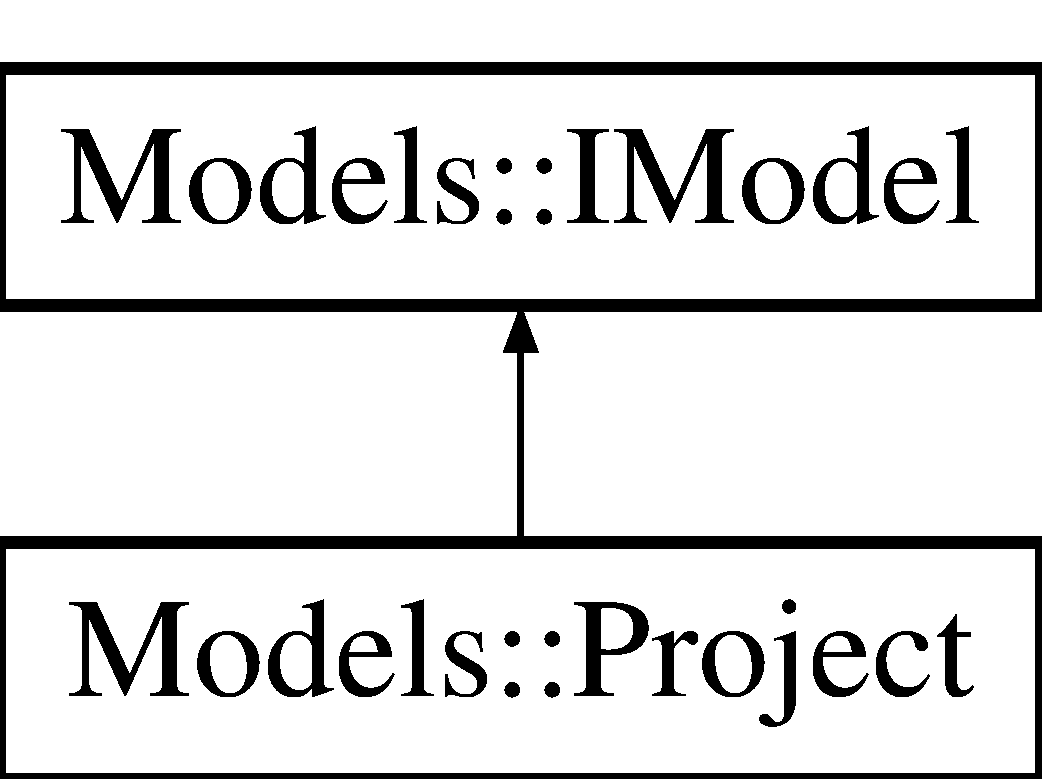
\includegraphics[height=2.000000cm]{dd/d3f/classModels_1_1Project}
\end{center}
\end{figure}
\subsection*{Public Member Functions}
\begin{DoxyCompactItemize}
\item 
\hypertarget{classModels_1_1Project_acd757cadcbeda1f4f83a2b0cd3c1cec1}{}\hyperlink{classModels_1_1Project_acd757cadcbeda1f4f83a2b0cd3c1cec1}{Project} ()\label{classModels_1_1Project_acd757cadcbeda1f4f83a2b0cd3c1cec1}

\begin{DoxyCompactList}\small\item\em \hyperlink{classModels_1_1Project_acd757cadcbeda1f4f83a2b0cd3c1cec1}{Project\+::\+Project} Construct a \hyperlink{classModels_1_1Project}{Project}. \end{DoxyCompactList}\item 
\hypertarget{classModels_1_1Project_a408d5fb64bb72b9492778b2ae26331f2}{}\hyperlink{classModels_1_1Project_a408d5fb64bb72b9492778b2ae26331f2}{Project} (Q\+String name)\label{classModels_1_1Project_a408d5fb64bb72b9492778b2ae26331f2}

\begin{DoxyCompactList}\small\item\em Project\+::project Construct a project with a name. \end{DoxyCompactList}\item 
\hyperlink{classModels_1_1Project_ac6c56b6ff24598135bc54d3b3edd3a47}{Project} (int id)
\begin{DoxyCompactList}\small\item\em \hyperlink{classModels_1_1Project_acd757cadcbeda1f4f83a2b0cd3c1cec1}{Project\+::\+Project} Construct a \hyperlink{classModels_1_1Project}{Project} which is specified by an {\itshape id} \end{DoxyCompactList}\item 
\hypertarget{classModels_1_1Project_a938f33016740cf7b33984d92ed932991}{}virtual \hyperlink{classModels_1_1Project_a938f33016740cf7b33984d92ed932991}{$\sim$\+Project} ()\label{classModels_1_1Project_a938f33016740cf7b33984d92ed932991}

\begin{DoxyCompactList}\small\item\em $\sim$\+Project Desctruct project object \end{DoxyCompactList}\item 
\hypertarget{classModels_1_1Project_afc167f2b5bf9c354826117c5057628ae}{}void \hyperlink{classModels_1_1Project_afc167f2b5bf9c354826117c5057628ae}{commit} ()\label{classModels_1_1Project_afc167f2b5bf9c354826117c5057628ae}

\begin{DoxyCompactList}\small\item\em \hyperlink{classModels_1_1Project_afc167f2b5bf9c354826117c5057628ae}{Project\+::commit} Update project data in the database. \end{DoxyCompactList}\item 
void \hyperlink{classModels_1_1Project_aa293709eeb68e4271cac8d4cce418ffa}{hydrat} (int id)
\begin{DoxyCompactList}\small\item\em \hyperlink{classModels_1_1Project_aa293709eeb68e4271cac8d4cce418ffa}{Project\+::hydrat} Insert project data which is specified by {\itshape id} in the database. \end{DoxyCompactList}\item 
\hypertarget{classModels_1_1Project_ab55c71c009ae796e7dbe03017fed67ee}{}void \hyperlink{classModels_1_1Project_ab55c71c009ae796e7dbe03017fed67ee}{remove} ()\label{classModels_1_1Project_ab55c71c009ae796e7dbe03017fed67ee}

\begin{DoxyCompactList}\small\item\em \hyperlink{classModels_1_1Project_ab55c71c009ae796e7dbe03017fed67ee}{Project\+::remove} Remove the current project. \end{DoxyCompactList}\item 
Q\+Variant\+Hash \hyperlink{classModels_1_1Project_a7db5156657a7dbadd024aead14a40182}{get\+Data\+Map} ()
\begin{DoxyCompactList}\small\item\em get\+Data\+Map Get all data of model with a Hash\+Map key/value \end{DoxyCompactList}\item 
Q\+String \hyperlink{classModels_1_1Project_a11d3b85bdc38daba928bfbfd962a0e32}{get\+Name} () const 
\begin{DoxyCompactList}\small\item\em \hyperlink{classModels_1_1Project_a11d3b85bdc38daba928bfbfd962a0e32}{Project\+::get\+Name} Return the project name. \end{DoxyCompactList}\item 
void \hyperlink{classModels_1_1Project_ac5ffa6ff6d31647fd880881257f47889}{set\+Name} (const Q\+String \&name)
\begin{DoxyCompactList}\small\item\em \hyperlink{classModels_1_1Project_ac5ffa6ff6d31647fd880881257f47889}{Project\+::set\+Name} Modify the project {\itshape name} \end{DoxyCompactList}\item 
Q\+String \hyperlink{classModels_1_1Project_a065b9cd68962c78302a84c686e10ae13}{get\+Description} () const 
\begin{DoxyCompactList}\small\item\em \hyperlink{classModels_1_1Project_a065b9cd68962c78302a84c686e10ae13}{Project\+::get\+Description} Return a project description. \end{DoxyCompactList}\item 
void \hyperlink{classModels_1_1Project_a2cccaca77bff95f13b3320f3f03dc9e7}{set\+Description} (const Q\+String \&description)
\begin{DoxyCompactList}\small\item\em \hyperlink{classModels_1_1Project_a2cccaca77bff95f13b3320f3f03dc9e7}{Project\+::set\+Description} Modify the project {\itshape description} \end{DoxyCompactList}\item 
Q\+Date \hyperlink{classModels_1_1Project_a31b8e46aabb1327499f7e36f170900e3}{get\+Begin\+Date} () const 
\begin{DoxyCompactList}\small\item\em \hyperlink{classModels_1_1Project_a31b8e46aabb1327499f7e36f170900e3}{Project\+::get\+Begin\+Date} return the date of creation of the {\bfseries \hyperlink{classModels_1_1Project}{Project}} \end{DoxyCompactList}\item 
void \hyperlink{classModels_1_1Project_a07dfb00cbec7442197a91bc0795ab14d}{set\+Begin\+Date} (Q\+Date begin\+Date)
\begin{DoxyCompactList}\small\item\em \hyperlink{classModels_1_1Project_a07dfb00cbec7442197a91bc0795ab14d}{Project\+::set\+Begin\+Date} Modify {\itshape begin\+Date} of a {\bfseries \hyperlink{classModels_1_1Project}{Project}} \end{DoxyCompactList}\item 
Q\+Date \hyperlink{classModels_1_1Project_aaf6792d15dcd65c3708e4a01b80e3108}{get\+End\+Date} () const 
\begin{DoxyCompactList}\small\item\em \hyperlink{classModels_1_1Project_aaf6792d15dcd65c3708e4a01b80e3108}{Project\+::get\+End\+Date} Return the {\itshape end\+Date} of the {\bfseries \hyperlink{classModels_1_1Project}{Project}} \end{DoxyCompactList}\item 
void \hyperlink{classModels_1_1Project_a89e9603b862d0a282e4eb03e122e8c05}{set\+End\+Date} (Q\+Date end\+Date)
\begin{DoxyCompactList}\small\item\em \hyperlink{classModels_1_1Project_a89e9603b862d0a282e4eb03e122e8c05}{Project\+::set\+End\+Date} Modify {\itshape end\+Date} of {\bfseries \hyperlink{classModels_1_1Project}{Project}} \end{DoxyCompactList}\item 
double \hyperlink{classModels_1_1Project_a6ad25c30f89821cd988a7ae92d84b41b}{get\+Cost} () const 
\begin{DoxyCompactList}\small\item\em \hyperlink{classModels_1_1Project_a6ad25c30f89821cd988a7ae92d84b41b}{Project\+::get\+Cost} Return the {\bfseries \hyperlink{classModels_1_1Project}{Project}} {\itshape cost} \end{DoxyCompactList}\item 
void \hyperlink{classModels_1_1Project_a840437ed81c595608bd285cac4065082}{set\+Cost} (double cost)
\begin{DoxyCompactList}\small\item\em \hyperlink{classModels_1_1Project_a840437ed81c595608bd285cac4065082}{Project\+::set\+Cost} Modify the {\bfseries \hyperlink{classModels_1_1Project}{Project}} {\itshape cost} \end{DoxyCompactList}\item 
double \hyperlink{classModels_1_1Project_a46d74a7452e712d223f1ca444a4cc180}{get\+Daily\+Rate} () const 
\begin{DoxyCompactList}\small\item\em \hyperlink{classModels_1_1Project_a46d74a7452e712d223f1ca444a4cc180}{Project\+::get\+Daily\+Rate} Return the daily rate estimated for this project. \end{DoxyCompactList}\item 
void \hyperlink{classModels_1_1Project_a9bc03d9632334a550bd25f6286d2c7a2}{set\+Daily\+Rate} (double daily\+Rate)
\begin{DoxyCompactList}\small\item\em \hyperlink{classModels_1_1Project_a9bc03d9632334a550bd25f6286d2c7a2}{Project\+::set\+Daily\+Rate} Modify the daily rate {\itshape daily\+Rate} of the current project. \end{DoxyCompactList}\item 
Q\+Shared\+Pointer$<$ \hyperlink{classModels_1_1Customer}{Customer} $>$ \hyperlink{classModels_1_1Project_ad15f442a24c9d42144b73f27a7afaa35}{get\+Customer} () const 
\begin{DoxyCompactList}\small\item\em \hyperlink{classModels_1_1Project_ad15f442a24c9d42144b73f27a7afaa35}{Project\+::get\+Customer} Return the reference to the customer linked to this project. \end{DoxyCompactList}\item 
void \hyperlink{classModels_1_1Project_a9d305edf054735b911e144516d3eccba}{set\+Customer} (Q\+Shared\+Pointer$<$ \hyperlink{classModels_1_1Customer}{Customer} $>$ customer)
\begin{DoxyCompactList}\small\item\em \hyperlink{classModels_1_1Project_a9d305edf054735b911e144516d3eccba}{Project\+::set\+Customer} Modify the {\itshape customer} linked to this project. \end{DoxyCompactList}\item 
bool \hyperlink{classModels_1_1Project_a2f322e63f6b42273c24093b9df46c2d6}{operator==} (const \hyperlink{classModels_1_1Project}{Project} \&p)
\begin{DoxyCompactList}\small\item\em \hyperlink{classModels_1_1Project_a2f322e63f6b42273c24093b9df46c2d6}{Project\+::operator ==} Re-\/define the operator \char`\"{}==\char`\"{} to compare if the current project is the same to the other {\bfseries \hyperlink{classModels_1_1Project}{Project}} {\itshape p} Return T\+R\+U\+E if both projects are the same, else F\+A\+L\+S\+E. \end{DoxyCompactList}\item 
bool \hyperlink{classModels_1_1Project_a8e7cc264d433c708323faccae7bdd082}{operator$<$} (const \hyperlink{classModels_1_1Project}{Project} \&p) const 
\begin{DoxyCompactList}\small\item\em \hyperlink{classModels_1_1Project_a8e7cc264d433c708323faccae7bdd082}{Project\+::operator $<$} defines the operator "$<$ to compare two {\bfseries \hyperlink{classModels_1_1Project}{Project}} and to see if the fisrt is anterior to the second. \end{DoxyCompactList}\item 
bool \hyperlink{classModels_1_1Project_adf5947680a4eca62cd1cbda58a2a62f0}{operator!=} (const \hyperlink{classModels_1_1Project}{Project} \&p)
\begin{DoxyCompactList}\small\item\em \hyperlink{classModels_1_1Project_a2f322e63f6b42273c24093b9df46c2d6}{Project\+::operator ==} Re-\/define the operator \char`\"{}!=\char`\"{} to compare if the current project is differnt to the other {\bfseries \hyperlink{classModels_1_1Project}{Project}} {\itshape p} Return T\+R\+U\+E if both projects are different, else F\+A\+L\+S\+E. \end{DoxyCompactList}\item 
double \hyperlink{classModels_1_1Project_abadcaa9256589f11535114a2ab3464d6}{get\+Cost} ()
\begin{DoxyCompactList}\small\item\em Project\+::cost\+Compute compute the {\bfseries \hyperlink{classModels_1_1Project}{Project}} {\itshape cost} \end{DoxyCompactList}\end{DoxyCompactItemize}
\subsection*{Additional Inherited Members}


\subsection{Detailed Description}
The \hyperlink{classModels_1_1Project}{Project} class \+: \hyperlink{classModels_1_1Project}{Project} linked to a \hyperlink{classModels_1_1Customer}{Customer}. 

\begin{DoxyAuthor}{Author}
Florent Berbie 
\end{DoxyAuthor}
\begin{DoxySeeAlso}{See also}
\hyperlink{classModels_1_1IModel}{I\+Model} 
\end{DoxySeeAlso}


\subsection{Constructor \& Destructor Documentation}
\hypertarget{classModels_1_1Project_ac6c56b6ff24598135bc54d3b3edd3a47}{}\index{Models\+::\+Project@{Models\+::\+Project}!Project@{Project}}
\index{Project@{Project}!Models\+::\+Project@{Models\+::\+Project}}
\subsubsection[{Project}]{\setlength{\rightskip}{0pt plus 5cm}Models\+::\+Project\+::\+Project (
\begin{DoxyParamCaption}
\item[{int}]{id}
\end{DoxyParamCaption}
)}\label{classModels_1_1Project_ac6c56b6ff24598135bc54d3b3edd3a47}


\hyperlink{classModels_1_1Project_acd757cadcbeda1f4f83a2b0cd3c1cec1}{Project\+::\+Project} Construct a \hyperlink{classModels_1_1Project}{Project} which is specified by an {\itshape id} 


\begin{DoxyParams}{Parameters}
{\em id} & \\
\hline
\end{DoxyParams}


\subsection{Member Function Documentation}
\hypertarget{classModels_1_1Project_a31b8e46aabb1327499f7e36f170900e3}{}\index{Models\+::\+Project@{Models\+::\+Project}!get\+Begin\+Date@{get\+Begin\+Date}}
\index{get\+Begin\+Date@{get\+Begin\+Date}!Models\+::\+Project@{Models\+::\+Project}}
\subsubsection[{get\+Begin\+Date}]{\setlength{\rightskip}{0pt plus 5cm}Q\+Date Models\+::\+Project\+::get\+Begin\+Date (
\begin{DoxyParamCaption}
{}
\end{DoxyParamCaption}
) const}\label{classModels_1_1Project_a31b8e46aabb1327499f7e36f170900e3}


\hyperlink{classModels_1_1Project_a31b8e46aabb1327499f7e36f170900e3}{Project\+::get\+Begin\+Date} return the date of creation of the {\bfseries \hyperlink{classModels_1_1Project}{Project}} 

\begin{DoxyReturn}{Returns}
the begin date of the \hyperlink{classModels_1_1Project}{Project} 
\end{DoxyReturn}
\hypertarget{classModels_1_1Project_a6ad25c30f89821cd988a7ae92d84b41b}{}\index{Models\+::\+Project@{Models\+::\+Project}!get\+Cost@{get\+Cost}}
\index{get\+Cost@{get\+Cost}!Models\+::\+Project@{Models\+::\+Project}}
\subsubsection[{get\+Cost}]{\setlength{\rightskip}{0pt plus 5cm}double Models\+::\+Project\+::get\+Cost (
\begin{DoxyParamCaption}
{}
\end{DoxyParamCaption}
) const}\label{classModels_1_1Project_a6ad25c30f89821cd988a7ae92d84b41b}


\hyperlink{classModels_1_1Project_a6ad25c30f89821cd988a7ae92d84b41b}{Project\+::get\+Cost} Return the {\bfseries \hyperlink{classModels_1_1Project}{Project}} {\itshape cost} 

\begin{DoxyReturn}{Returns}
the project cost 
\end{DoxyReturn}
\hypertarget{classModels_1_1Project_abadcaa9256589f11535114a2ab3464d6}{}\index{Models\+::\+Project@{Models\+::\+Project}!get\+Cost@{get\+Cost}}
\index{get\+Cost@{get\+Cost}!Models\+::\+Project@{Models\+::\+Project}}
\subsubsection[{get\+Cost}]{\setlength{\rightskip}{0pt plus 5cm}double Models\+::\+Project\+::get\+Cost (
\begin{DoxyParamCaption}
{}
\end{DoxyParamCaption}
)}\label{classModels_1_1Project_abadcaa9256589f11535114a2ab3464d6}


Project\+::cost\+Compute compute the {\bfseries \hyperlink{classModels_1_1Project}{Project}} {\itshape cost} 

\begin{DoxyReturn}{Returns}
the project cost 
\end{DoxyReturn}
\hypertarget{classModels_1_1Project_ad15f442a24c9d42144b73f27a7afaa35}{}\index{Models\+::\+Project@{Models\+::\+Project}!get\+Customer@{get\+Customer}}
\index{get\+Customer@{get\+Customer}!Models\+::\+Project@{Models\+::\+Project}}
\subsubsection[{get\+Customer}]{\setlength{\rightskip}{0pt plus 5cm}Q\+Shared\+Pointer$<$ {\bf Customer} $>$ Models\+::\+Project\+::get\+Customer (
\begin{DoxyParamCaption}
{}
\end{DoxyParamCaption}
) const}\label{classModels_1_1Project_ad15f442a24c9d42144b73f27a7afaa35}


\hyperlink{classModels_1_1Project_ad15f442a24c9d42144b73f27a7afaa35}{Project\+::get\+Customer} Return the reference to the customer linked to this project. 

\begin{DoxyReturn}{Returns}
customer linked to this project 
\end{DoxyReturn}
\hypertarget{classModels_1_1Project_a46d74a7452e712d223f1ca444a4cc180}{}\index{Models\+::\+Project@{Models\+::\+Project}!get\+Daily\+Rate@{get\+Daily\+Rate}}
\index{get\+Daily\+Rate@{get\+Daily\+Rate}!Models\+::\+Project@{Models\+::\+Project}}
\subsubsection[{get\+Daily\+Rate}]{\setlength{\rightskip}{0pt plus 5cm}double Models\+::\+Project\+::get\+Daily\+Rate (
\begin{DoxyParamCaption}
{}
\end{DoxyParamCaption}
) const}\label{classModels_1_1Project_a46d74a7452e712d223f1ca444a4cc180}


\hyperlink{classModels_1_1Project_a46d74a7452e712d223f1ca444a4cc180}{Project\+::get\+Daily\+Rate} Return the daily rate estimated for this project. 

\begin{DoxyReturn}{Returns}
the daily rate linket to the current project 
\end{DoxyReturn}
\hypertarget{classModels_1_1Project_a7db5156657a7dbadd024aead14a40182}{}\index{Models\+::\+Project@{Models\+::\+Project}!get\+Data\+Map@{get\+Data\+Map}}
\index{get\+Data\+Map@{get\+Data\+Map}!Models\+::\+Project@{Models\+::\+Project}}
\subsubsection[{get\+Data\+Map}]{\setlength{\rightskip}{0pt plus 5cm}Q\+Variant\+Hash Models\+::\+Project\+::get\+Data\+Map (
\begin{DoxyParamCaption}
{}
\end{DoxyParamCaption}
)\hspace{0.3cm}{\ttfamily [virtual]}}\label{classModels_1_1Project_a7db5156657a7dbadd024aead14a40182}


get\+Data\+Map Get all data of model with a Hash\+Map key/value 

\begin{DoxyReturn}{Returns}
Model\textquotesingle{}s data 
\end{DoxyReturn}


Implements \hyperlink{classModels_1_1IModel_a9851b0f296aac58353edff22af11cf3c}{Models\+::\+I\+Model}.

\hypertarget{classModels_1_1Project_a065b9cd68962c78302a84c686e10ae13}{}\index{Models\+::\+Project@{Models\+::\+Project}!get\+Description@{get\+Description}}
\index{get\+Description@{get\+Description}!Models\+::\+Project@{Models\+::\+Project}}
\subsubsection[{get\+Description}]{\setlength{\rightskip}{0pt plus 5cm}Q\+String Models\+::\+Project\+::get\+Description (
\begin{DoxyParamCaption}
{}
\end{DoxyParamCaption}
) const}\label{classModels_1_1Project_a065b9cd68962c78302a84c686e10ae13}


\hyperlink{classModels_1_1Project_a065b9cd68962c78302a84c686e10ae13}{Project\+::get\+Description} Return a project description. 

\begin{DoxyReturn}{Returns}
project description 
\end{DoxyReturn}
\hypertarget{classModels_1_1Project_aaf6792d15dcd65c3708e4a01b80e3108}{}\index{Models\+::\+Project@{Models\+::\+Project}!get\+End\+Date@{get\+End\+Date}}
\index{get\+End\+Date@{get\+End\+Date}!Models\+::\+Project@{Models\+::\+Project}}
\subsubsection[{get\+End\+Date}]{\setlength{\rightskip}{0pt plus 5cm}Q\+Date Models\+::\+Project\+::get\+End\+Date (
\begin{DoxyParamCaption}
{}
\end{DoxyParamCaption}
) const}\label{classModels_1_1Project_aaf6792d15dcd65c3708e4a01b80e3108}


\hyperlink{classModels_1_1Project_aaf6792d15dcd65c3708e4a01b80e3108}{Project\+::get\+End\+Date} Return the {\itshape end\+Date} of the {\bfseries \hyperlink{classModels_1_1Project}{Project}} 

\begin{DoxyReturn}{Returns}
the end date of the project 
\end{DoxyReturn}
\hypertarget{classModels_1_1Project_a11d3b85bdc38daba928bfbfd962a0e32}{}\index{Models\+::\+Project@{Models\+::\+Project}!get\+Name@{get\+Name}}
\index{get\+Name@{get\+Name}!Models\+::\+Project@{Models\+::\+Project}}
\subsubsection[{get\+Name}]{\setlength{\rightskip}{0pt plus 5cm}Q\+String Models\+::\+Project\+::get\+Name (
\begin{DoxyParamCaption}
{}
\end{DoxyParamCaption}
) const}\label{classModels_1_1Project_a11d3b85bdc38daba928bfbfd962a0e32}


\hyperlink{classModels_1_1Project_a11d3b85bdc38daba928bfbfd962a0e32}{Project\+::get\+Name} Return the project name. 

\begin{DoxyReturn}{Returns}
project name 
\end{DoxyReturn}
\hypertarget{classModels_1_1Project_aa293709eeb68e4271cac8d4cce418ffa}{}\index{Models\+::\+Project@{Models\+::\+Project}!hydrat@{hydrat}}
\index{hydrat@{hydrat}!Models\+::\+Project@{Models\+::\+Project}}
\subsubsection[{hydrat}]{\setlength{\rightskip}{0pt plus 5cm}void Models\+::\+Project\+::hydrat (
\begin{DoxyParamCaption}
\item[{int}]{id}
\end{DoxyParamCaption}
)\hspace{0.3cm}{\ttfamily [virtual]}}\label{classModels_1_1Project_aa293709eeb68e4271cac8d4cce418ffa}


\hyperlink{classModels_1_1Project_aa293709eeb68e4271cac8d4cce418ffa}{Project\+::hydrat} Insert project data which is specified by {\itshape id} in the database. 


\begin{DoxyParams}{Parameters}
{\em id} & \hyperlink{classModels_1_1Project}{Project} identify \\
\hline
\end{DoxyParams}


Implements \hyperlink{classModels_1_1IModel_a7ce6def437f5e1f6a78ee1d67ca028e4}{Models\+::\+I\+Model}.

\hypertarget{classModels_1_1Project_adf5947680a4eca62cd1cbda58a2a62f0}{}\index{Models\+::\+Project@{Models\+::\+Project}!operator"!=@{operator"!=}}
\index{operator"!=@{operator"!=}!Models\+::\+Project@{Models\+::\+Project}}
\subsubsection[{operator"!=}]{\setlength{\rightskip}{0pt plus 5cm}bool Models\+::\+Project\+::operator!= (
\begin{DoxyParamCaption}
\item[{const {\bf Project} \&}]{p}
\end{DoxyParamCaption}
)}\label{classModels_1_1Project_adf5947680a4eca62cd1cbda58a2a62f0}


\hyperlink{classModels_1_1Project_a2f322e63f6b42273c24093b9df46c2d6}{Project\+::operator ==} Re-\/define the operator \char`\"{}!=\char`\"{} to compare if the current project is differnt to the other {\bfseries \hyperlink{classModels_1_1Project}{Project}} {\itshape p} Return T\+R\+U\+E if both projects are different, else F\+A\+L\+S\+E. 


\begin{DoxyParams}{Parameters}
{\em c} & \hyperlink{classModels_1_1Project}{Project} to compare \\
\hline
\end{DoxyParams}
\begin{DoxyReturn}{Returns}
boolean 
\end{DoxyReturn}
\hypertarget{classModels_1_1Project_a8e7cc264d433c708323faccae7bdd082}{}\index{Models\+::\+Project@{Models\+::\+Project}!operator$<$@{operator$<$}}
\index{operator$<$@{operator$<$}!Models\+::\+Project@{Models\+::\+Project}}
\subsubsection[{operator$<$}]{\setlength{\rightskip}{0pt plus 5cm}bool Models\+::\+Project\+::operator$<$ (
\begin{DoxyParamCaption}
\item[{const {\bf Project} \&}]{p}
\end{DoxyParamCaption}
) const}\label{classModels_1_1Project_a8e7cc264d433c708323faccae7bdd082}


\hyperlink{classModels_1_1Project_a8e7cc264d433c708323faccae7bdd082}{Project\+::operator $<$} defines the operator "$<$ to compare two {\bfseries \hyperlink{classModels_1_1Project}{Project}} and to see if the fisrt is anterior to the second. 


\begin{DoxyParams}{Parameters}
{\em b} & the {\bfseries \hyperlink{classModels_1_1Project}{Project}} to compare with the current {\bfseries \hyperlink{classModels_1_1Project}{Project}} \\
\hline
\end{DoxyParams}
\begin{DoxyReturn}{Returns}
true if the {\bfseries \hyperlink{classModels_1_1Project}{Project}} are different else false 
\end{DoxyReturn}
\hypertarget{classModels_1_1Project_a2f322e63f6b42273c24093b9df46c2d6}{}\index{Models\+::\+Project@{Models\+::\+Project}!operator==@{operator==}}
\index{operator==@{operator==}!Models\+::\+Project@{Models\+::\+Project}}
\subsubsection[{operator==}]{\setlength{\rightskip}{0pt plus 5cm}bool Models\+::\+Project\+::operator== (
\begin{DoxyParamCaption}
\item[{const {\bf Project} \&}]{p}
\end{DoxyParamCaption}
)}\label{classModels_1_1Project_a2f322e63f6b42273c24093b9df46c2d6}


\hyperlink{classModels_1_1Project_a2f322e63f6b42273c24093b9df46c2d6}{Project\+::operator ==} Re-\/define the operator \char`\"{}==\char`\"{} to compare if the current project is the same to the other {\bfseries \hyperlink{classModels_1_1Project}{Project}} {\itshape p} Return T\+R\+U\+E if both projects are the same, else F\+A\+L\+S\+E. 


\begin{DoxyParams}{Parameters}
{\em c} & \hyperlink{classModels_1_1Project}{Project} to compare \\
\hline
\end{DoxyParams}
\begin{DoxyReturn}{Returns}
boolean 
\end{DoxyReturn}
\hypertarget{classModels_1_1Project_a07dfb00cbec7442197a91bc0795ab14d}{}\index{Models\+::\+Project@{Models\+::\+Project}!set\+Begin\+Date@{set\+Begin\+Date}}
\index{set\+Begin\+Date@{set\+Begin\+Date}!Models\+::\+Project@{Models\+::\+Project}}
\subsubsection[{set\+Begin\+Date}]{\setlength{\rightskip}{0pt plus 5cm}void Models\+::\+Project\+::set\+Begin\+Date (
\begin{DoxyParamCaption}
\item[{Q\+Date}]{begin\+Date}
\end{DoxyParamCaption}
)}\label{classModels_1_1Project_a07dfb00cbec7442197a91bc0795ab14d}


\hyperlink{classModels_1_1Project_a07dfb00cbec7442197a91bc0795ab14d}{Project\+::set\+Begin\+Date} Modify {\itshape begin\+Date} of a {\bfseries \hyperlink{classModels_1_1Project}{Project}} 


\begin{DoxyParams}{Parameters}
{\em begin\+Date} & the new date of creation of the project \\
\hline
\end{DoxyParams}
\hypertarget{classModels_1_1Project_a840437ed81c595608bd285cac4065082}{}\index{Models\+::\+Project@{Models\+::\+Project}!set\+Cost@{set\+Cost}}
\index{set\+Cost@{set\+Cost}!Models\+::\+Project@{Models\+::\+Project}}
\subsubsection[{set\+Cost}]{\setlength{\rightskip}{0pt plus 5cm}void Models\+::\+Project\+::set\+Cost (
\begin{DoxyParamCaption}
\item[{double}]{cost}
\end{DoxyParamCaption}
)}\label{classModels_1_1Project_a840437ed81c595608bd285cac4065082}


\hyperlink{classModels_1_1Project_a840437ed81c595608bd285cac4065082}{Project\+::set\+Cost} Modify the {\bfseries \hyperlink{classModels_1_1Project}{Project}} {\itshape cost} 


\begin{DoxyParams}{Parameters}
{\em cost} & the project\+Cost \\
\hline
\end{DoxyParams}
\hypertarget{classModels_1_1Project_a9d305edf054735b911e144516d3eccba}{}\index{Models\+::\+Project@{Models\+::\+Project}!set\+Customer@{set\+Customer}}
\index{set\+Customer@{set\+Customer}!Models\+::\+Project@{Models\+::\+Project}}
\subsubsection[{set\+Customer}]{\setlength{\rightskip}{0pt plus 5cm}void Models\+::\+Project\+::set\+Customer (
\begin{DoxyParamCaption}
\item[{Q\+Shared\+Pointer$<$ {\bf Customer} $>$}]{customer}
\end{DoxyParamCaption}
)}\label{classModels_1_1Project_a9d305edf054735b911e144516d3eccba}


\hyperlink{classModels_1_1Project_a9d305edf054735b911e144516d3eccba}{Project\+::set\+Customer} Modify the {\itshape customer} linked to this project. 


\begin{DoxyParams}{Parameters}
{\em customer} & New customer associated to this project \\
\hline
\end{DoxyParams}
\hypertarget{classModels_1_1Project_a9bc03d9632334a550bd25f6286d2c7a2}{}\index{Models\+::\+Project@{Models\+::\+Project}!set\+Daily\+Rate@{set\+Daily\+Rate}}
\index{set\+Daily\+Rate@{set\+Daily\+Rate}!Models\+::\+Project@{Models\+::\+Project}}
\subsubsection[{set\+Daily\+Rate}]{\setlength{\rightskip}{0pt plus 5cm}void Models\+::\+Project\+::set\+Daily\+Rate (
\begin{DoxyParamCaption}
\item[{double}]{daily\+Rate}
\end{DoxyParamCaption}
)}\label{classModels_1_1Project_a9bc03d9632334a550bd25f6286d2c7a2}


\hyperlink{classModels_1_1Project_a9bc03d9632334a550bd25f6286d2c7a2}{Project\+::set\+Daily\+Rate} Modify the daily rate {\itshape daily\+Rate} of the current project. 


\begin{DoxyParams}{Parameters}
{\em daily\+Rate} & New daily rate associated to the current project \\
\hline
\end{DoxyParams}
\hypertarget{classModels_1_1Project_a2cccaca77bff95f13b3320f3f03dc9e7}{}\index{Models\+::\+Project@{Models\+::\+Project}!set\+Description@{set\+Description}}
\index{set\+Description@{set\+Description}!Models\+::\+Project@{Models\+::\+Project}}
\subsubsection[{set\+Description}]{\setlength{\rightskip}{0pt plus 5cm}void Models\+::\+Project\+::set\+Description (
\begin{DoxyParamCaption}
\item[{const Q\+String \&}]{description}
\end{DoxyParamCaption}
)}\label{classModels_1_1Project_a2cccaca77bff95f13b3320f3f03dc9e7}


\hyperlink{classModels_1_1Project_a2cccaca77bff95f13b3320f3f03dc9e7}{Project\+::set\+Description} Modify the project {\itshape description} 


\begin{DoxyParams}{Parameters}
{\em description} & New project description \\
\hline
\end{DoxyParams}
\hypertarget{classModels_1_1Project_a89e9603b862d0a282e4eb03e122e8c05}{}\index{Models\+::\+Project@{Models\+::\+Project}!set\+End\+Date@{set\+End\+Date}}
\index{set\+End\+Date@{set\+End\+Date}!Models\+::\+Project@{Models\+::\+Project}}
\subsubsection[{set\+End\+Date}]{\setlength{\rightskip}{0pt plus 5cm}void Models\+::\+Project\+::set\+End\+Date (
\begin{DoxyParamCaption}
\item[{Q\+Date}]{end\+Date}
\end{DoxyParamCaption}
)}\label{classModels_1_1Project_a89e9603b862d0a282e4eb03e122e8c05}


\hyperlink{classModels_1_1Project_a89e9603b862d0a282e4eb03e122e8c05}{Project\+::set\+End\+Date} Modify {\itshape end\+Date} of {\bfseries \hyperlink{classModels_1_1Project}{Project}} 


\begin{DoxyParams}{Parameters}
{\em end\+Date} & the new end date of the project \\
\hline
\end{DoxyParams}
\hypertarget{classModels_1_1Project_ac5ffa6ff6d31647fd880881257f47889}{}\index{Models\+::\+Project@{Models\+::\+Project}!set\+Name@{set\+Name}}
\index{set\+Name@{set\+Name}!Models\+::\+Project@{Models\+::\+Project}}
\subsubsection[{set\+Name}]{\setlength{\rightskip}{0pt plus 5cm}void Models\+::\+Project\+::set\+Name (
\begin{DoxyParamCaption}
\item[{const Q\+String \&}]{name}
\end{DoxyParamCaption}
)}\label{classModels_1_1Project_ac5ffa6ff6d31647fd880881257f47889}


\hyperlink{classModels_1_1Project_ac5ffa6ff6d31647fd880881257f47889}{Project\+::set\+Name} Modify the project {\itshape name} 


\begin{DoxyParams}{Parameters}
{\em name} & \hyperlink{classModels_1_1Project}{Project} name \\
\hline
\end{DoxyParams}


The documentation for this class was generated from the following files\+:\begin{DoxyCompactItemize}
\item 
src/models/project.\+h\item 
src/models/project.\+cpp\end{DoxyCompactItemize}

\hypertarget{classGui_1_1Widgets_1_1Delegates_1_1ProjectComboDelegate}{\section{Gui\-:\-:Widgets\-:\-:Delegates\-:\-:Project\-Combo\-Delegate Class Reference}
\label{classGui_1_1Widgets_1_1Delegates_1_1ProjectComboDelegate}\index{Gui\-::\-Widgets\-::\-Delegates\-::\-Project\-Combo\-Delegate@{Gui\-::\-Widgets\-::\-Delegates\-::\-Project\-Combo\-Delegate}}
}
Inheritance diagram for Gui\-:\-:Widgets\-:\-:Delegates\-:\-:Project\-Combo\-Delegate\-:\begin{figure}[H]
\begin{center}
\leavevmode
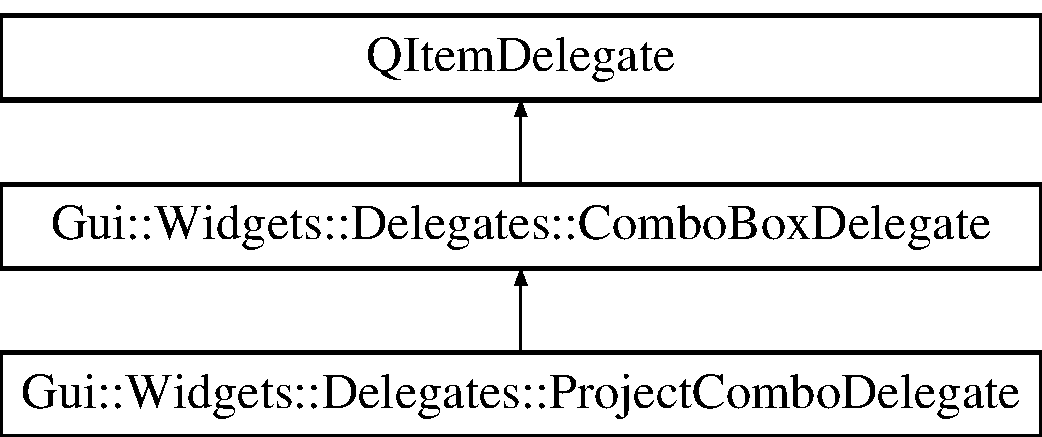
\includegraphics[height=3.000000cm]{d6/d93/classGui_1_1Widgets_1_1Delegates_1_1ProjectComboDelegate}
\end{center}
\end{figure}
\subsection*{Public Member Functions}
\begin{DoxyCompactItemize}
\item 
\hypertarget{classGui_1_1Widgets_1_1Delegates_1_1ProjectComboDelegate_a5fda87c3db87a0928717810a0ac2812f}{{\bfseries Project\-Combo\-Delegate} (Q\-Shared\-Pointer$<$ \hyperlink{classModels_1_1Customer}{Models\-::\-Customer} $>$ c, Q\-Object $\ast$parent=0)}\label{classGui_1_1Widgets_1_1Delegates_1_1ProjectComboDelegate_a5fda87c3db87a0928717810a0ac2812f}

\item 
\hypertarget{classGui_1_1Widgets_1_1Delegates_1_1ProjectComboDelegate_adbfc28a3e6de34dc63d7290ae5b5c053}{Q\-Widget $\ast$ {\bfseries create\-Editor} (Q\-Widget $\ast$parent, const Q\-Style\-Option\-View\-Item \&option, const Q\-Model\-Index \&index) const }\label{classGui_1_1Widgets_1_1Delegates_1_1ProjectComboDelegate_adbfc28a3e6de34dc63d7290ae5b5c053}

\item 
\hypertarget{classGui_1_1Widgets_1_1Delegates_1_1ProjectComboDelegate_a20cbc84d26b83083fdf7efecae3407cf}{void {\bfseries paint} (Q\-Painter $\ast$painter, const Q\-Style\-Option\-View\-Item \&option, const Q\-Model\-Index \&index) const }\label{classGui_1_1Widgets_1_1Delegates_1_1ProjectComboDelegate_a20cbc84d26b83083fdf7efecae3407cf}

\item 
\hypertarget{classGui_1_1Widgets_1_1Delegates_1_1ProjectComboDelegate_a7e14627b3942a96f190e31a4e67edc95}{void {\bfseries remove\-In\-Combo} (Q\-List$<$ int $>$ \&)}\label{classGui_1_1Widgets_1_1Delegates_1_1ProjectComboDelegate_a7e14627b3942a96f190e31a4e67edc95}

\item 
\hypertarget{classGui_1_1Widgets_1_1Delegates_1_1ProjectComboDelegate_a63d0ef3a5179d72ab577f359c8f7a6fa}{Q\-Map$<$ int, \hyperlink{classModels_1_1Project}{Models\-::\-Project} $>$ {\bfseries get\-Projects} () const }\label{classGui_1_1Widgets_1_1Delegates_1_1ProjectComboDelegate_a63d0ef3a5179d72ab577f359c8f7a6fa}

\item 
\hypertarget{classGui_1_1Widgets_1_1Delegates_1_1ProjectComboDelegate_ad07bf1e09c752159161a3f585c61b4d7}{bool {\bfseries get\-Locked} () const }\label{classGui_1_1Widgets_1_1Delegates_1_1ProjectComboDelegate_ad07bf1e09c752159161a3f585c61b4d7}

\item 
\hypertarget{classGui_1_1Widgets_1_1Delegates_1_1ProjectComboDelegate_ac93369dde11856d4097851f7f1158f48}{void {\bfseries set\-Locked} (bool get\-Llocked)}\label{classGui_1_1Widgets_1_1Delegates_1_1ProjectComboDelegate_ac93369dde11856d4097851f7f1158f48}

\end{DoxyCompactItemize}


The documentation for this class was generated from the following files\-:\begin{DoxyCompactItemize}
\item 
/home/travis/build/\-F\-A\-C\-T-\/\-Team/\-Fact\-Dev/src/gui/widgets/delegates/projectcombodelegate.\-h\item 
/home/travis/build/\-F\-A\-C\-T-\/\-Team/\-Fact\-Dev/src/gui/widgets/delegates/projectcombodelegate.\-cpp\end{DoxyCompactItemize}

\hypertarget{classDatabase_1_1ProjectDatabase}{\section{Database\+:\+:Project\+Database Class Reference}
\label{classDatabase_1_1ProjectDatabase}\index{Database\+::\+Project\+Database@{Database\+::\+Project\+Database}}
}


The \hyperlink{classDatabase_1_1ProjectDatabase}{Project\+Database} class Project table database.  




{\ttfamily \#include $<$projectdatabase.\+h$>$}

Inheritance diagram for Database\+:\+:Project\+Database\+:\begin{figure}[H]
\begin{center}
\leavevmode
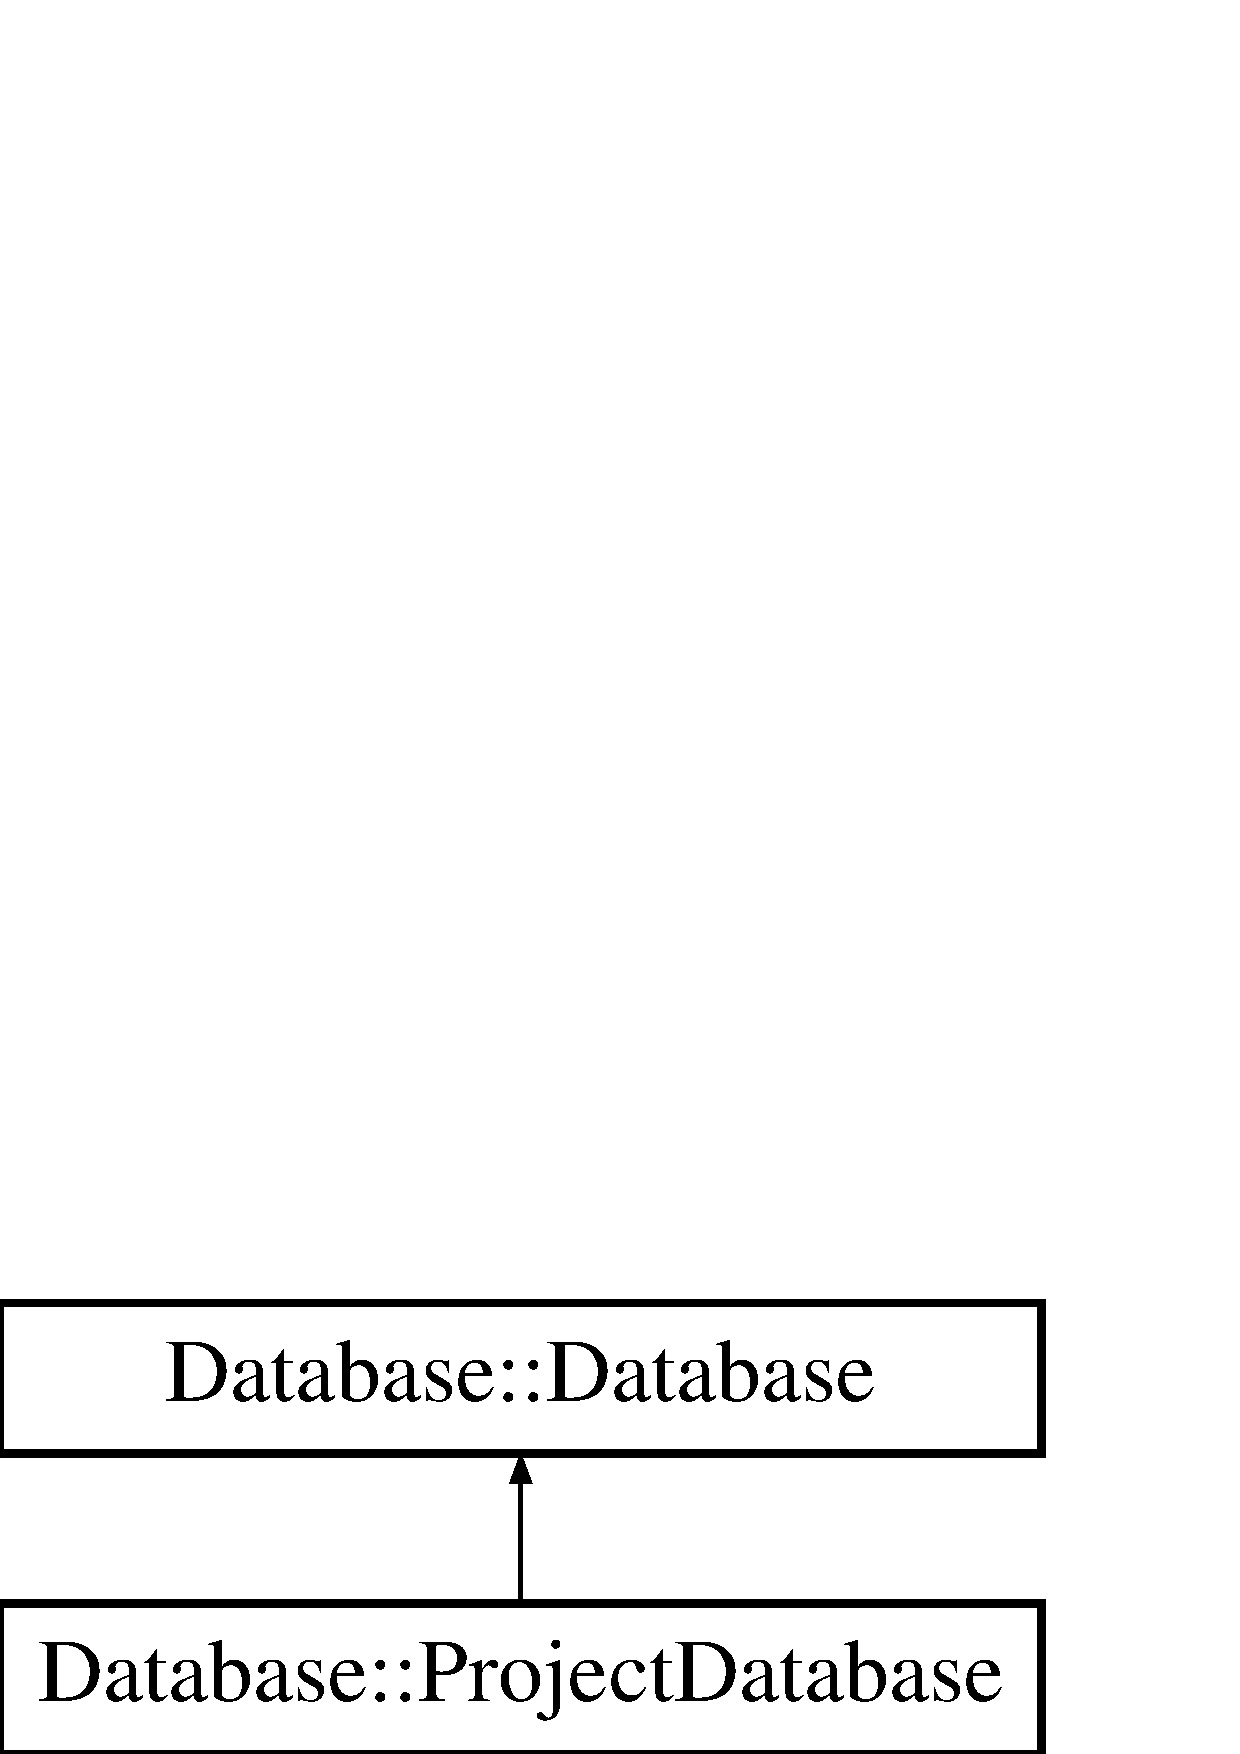
\includegraphics[height=2.000000cm]{dd/dbf/classDatabase_1_1ProjectDatabase}
\end{center}
\end{figure}
\subsection*{Public Member Functions}
\begin{DoxyCompactItemize}
\item 
\hyperlink{classModels_1_1Project}{Models\+::\+Project} $\ast$ \hyperlink{classDatabase_1_1ProjectDatabase_ae656663ce7e517e13815198f66341b2a}{get\+Project} (const int p\+Id)
\begin{DoxyCompactList}\small\item\em Project\+Databaseget\+Project Get informations about the project identified by 'p\+Id'. \end{DoxyCompactList}\item 
int \hyperlink{classDatabase_1_1ProjectDatabase_a904588d19669d5e391518a946fd94ddf}{add\+Project} (const \hyperlink{classModels_1_1Project}{Models\+::\+Project} \&)
\begin{DoxyCompactList}\small\item\em \hyperlink{classDatabase_1_1ProjectDatabase}{Project\+Database}\+:add\+Project Add the project 'p\+Project' to the database. \end{DoxyCompactList}\item 
\hypertarget{classDatabase_1_1ProjectDatabase_a5a839ed196050cf41a1b0f1073757599}{void \hyperlink{classDatabase_1_1ProjectDatabase_a5a839ed196050cf41a1b0f1073757599}{update\+Project} (const \hyperlink{classModels_1_1Project}{Models\+::\+Project} \&)}\label{classDatabase_1_1ProjectDatabase_a5a839ed196050cf41a1b0f1073757599}

\begin{DoxyCompactList}\small\item\em \hyperlink{classDatabase_1_1ProjectDatabase}{Project\+Database}\+:update\+Project Update informations about the project. \end{DoxyCompactList}\item 
void \hyperlink{classDatabase_1_1ProjectDatabase_a45fb24373d53e060d05cb166cd635370}{remove\+Project} (const int p\+Id)
\begin{DoxyCompactList}\small\item\em remove\+Project Remove the project with the id 'p\+Id' \end{DoxyCompactList}\item 
int \hyperlink{classDatabase_1_1ProjectDatabase_a57f293ea89b06e1cefff8189a5dc9444}{get\+Nb\+Projects} ()
\begin{DoxyCompactList}\small\item\em \hyperlink{classDatabase_1_1ProjectDatabase}{Project\+Database}\+:get\+Nb\+Projects Return the number of projects existing. \end{DoxyCompactList}\item 
int \hyperlink{classDatabase_1_1ProjectDatabase_a9d86e98ae77eaef7875c36c84e08722b}{get\+Nb\+Projects\+For\+A\+Customer} (const int p\+Id)
\begin{DoxyCompactList}\small\item\em \hyperlink{classDatabase_1_1ProjectDatabase}{Project\+Database}\+:get\+Nb\+Projects\+For\+A\+Customer Return the number of projects existing for an identify customer {\itshape p\+Id} \end{DoxyCompactList}\item 
Q\+Map$<$ int, \hyperlink{classModels_1_1Project}{Models\+::\+Project} $>$ \hyperlink{classDatabase_1_1ProjectDatabase_a1bbdbcb01b9741800e49902d0783e5f3}{get\+Projects\+Of\+Customer} (Q\+Shared\+Pointer$<$ \hyperlink{classModels_1_1Customer}{Models\+::\+Customer} $>$ c)
\begin{DoxyCompactList}\small\item\em get\+Projects\+Of\+Customer Return all projects of a customer \end{DoxyCompactList}\item 
Q\+Standard\+Item\+Model $\ast$ \hyperlink{classDatabase_1_1ProjectDatabase_ad2da7cde75b3b84dcdf2771969950ae9}{get\+Projects\+Table} (const int p\+Id)  throw (\+Db\+Exception$\ast$)
\begin{DoxyCompactList}\small\item\em get\+Projects\+Table Return all projects of a customer in Q\+Standard\+Item\+Model \end{DoxyCompactList}\item 
\hyperlink{classModels_1_1Project}{Models\+::\+Project} $\ast$ \hyperlink{classDatabase_1_1ProjectDatabase_a360d570a10c3e9df38241a650e1a30a6}{get\+Project} (Q\+Sql\+Query \&q)
\begin{DoxyCompactList}\small\item\em get\+Project Obtain a project without new query \end{DoxyCompactList}\end{DoxyCompactItemize}
\subsection*{Static Public Member Functions}
\begin{DoxyCompactItemize}
\item 
static \hyperlink{classDatabase_1_1ProjectDatabase}{Project\+Database} $\ast$ \hyperlink{classDatabase_1_1ProjectDatabase_a051359f2f1390cbdd3c47b1044ab166f}{instance} ()  throw (\+Db\+Exception$\ast$)
\begin{DoxyCompactList}\small\item\em Project\+Database\+::get\+Instance Return an instance of \hyperlink{classDatabase_1_1ProjectDatabase}{Project\+Database}. \end{DoxyCompactList}\end{DoxyCompactItemize}
\subsection*{Additional Inherited Members}


\subsection{Detailed Description}
The \hyperlink{classDatabase_1_1ProjectDatabase}{Project\+Database} class Project table database. 

\begin{DoxyAuthor}{Author}
Florent Berbie 
\end{DoxyAuthor}
\begin{DoxySeeAlso}{See also}
\hyperlink{classDatabase_1_1Database}{Database} 

Project 
\end{DoxySeeAlso}


\subsection{Member Function Documentation}
\hypertarget{classDatabase_1_1ProjectDatabase_a904588d19669d5e391518a946fd94ddf}{\index{Database\+::\+Project\+Database@{Database\+::\+Project\+Database}!add\+Project@{add\+Project}}
\index{add\+Project@{add\+Project}!Database\+::\+Project\+Database@{Database\+::\+Project\+Database}}
\subsubsection[{add\+Project}]{\setlength{\rightskip}{0pt plus 5cm}int Database\+::\+Project\+Database\+::add\+Project (
\begin{DoxyParamCaption}
\item[{const {\bf Models\+::\+Project} \&}]{p\+Project}
\end{DoxyParamCaption}
)}}\label{classDatabase_1_1ProjectDatabase_a904588d19669d5e391518a946fd94ddf}


\hyperlink{classDatabase_1_1ProjectDatabase}{Project\+Database}\+:add\+Project Add the project 'p\+Project' to the database. 

\begin{DoxyReturn}{Returns}
project id 
\end{DoxyReturn}
\hypertarget{classDatabase_1_1ProjectDatabase_a57f293ea89b06e1cefff8189a5dc9444}{\index{Database\+::\+Project\+Database@{Database\+::\+Project\+Database}!get\+Nb\+Projects@{get\+Nb\+Projects}}
\index{get\+Nb\+Projects@{get\+Nb\+Projects}!Database\+::\+Project\+Database@{Database\+::\+Project\+Database}}
\subsubsection[{get\+Nb\+Projects}]{\setlength{\rightskip}{0pt plus 5cm}int Database\+::\+Project\+Database\+::get\+Nb\+Projects (
\begin{DoxyParamCaption}
{}
\end{DoxyParamCaption}
)}}\label{classDatabase_1_1ProjectDatabase_a57f293ea89b06e1cefff8189a5dc9444}


\hyperlink{classDatabase_1_1ProjectDatabase}{Project\+Database}\+:get\+Nb\+Projects Return the number of projects existing. 

\begin{DoxyReturn}{Returns}
number of projects 
\end{DoxyReturn}
\hypertarget{classDatabase_1_1ProjectDatabase_a9d86e98ae77eaef7875c36c84e08722b}{\index{Database\+::\+Project\+Database@{Database\+::\+Project\+Database}!get\+Nb\+Projects\+For\+A\+Customer@{get\+Nb\+Projects\+For\+A\+Customer}}
\index{get\+Nb\+Projects\+For\+A\+Customer@{get\+Nb\+Projects\+For\+A\+Customer}!Database\+::\+Project\+Database@{Database\+::\+Project\+Database}}
\subsubsection[{get\+Nb\+Projects\+For\+A\+Customer}]{\setlength{\rightskip}{0pt plus 5cm}int Database\+::\+Project\+Database\+::get\+Nb\+Projects\+For\+A\+Customer (
\begin{DoxyParamCaption}
\item[{const int}]{p\+Id}
\end{DoxyParamCaption}
)}}\label{classDatabase_1_1ProjectDatabase_a9d86e98ae77eaef7875c36c84e08722b}


\hyperlink{classDatabase_1_1ProjectDatabase}{Project\+Database}\+:get\+Nb\+Projects\+For\+A\+Customer Return the number of projects existing for an identify customer {\itshape p\+Id} 


\begin{DoxyParams}{Parameters}
{\em p\+Id} & Project id \\
\hline
\end{DoxyParams}
\begin{DoxyReturn}{Returns}
number of projects 
\end{DoxyReturn}
\hypertarget{classDatabase_1_1ProjectDatabase_ae656663ce7e517e13815198f66341b2a}{\index{Database\+::\+Project\+Database@{Database\+::\+Project\+Database}!get\+Project@{get\+Project}}
\index{get\+Project@{get\+Project}!Database\+::\+Project\+Database@{Database\+::\+Project\+Database}}
\subsubsection[{get\+Project}]{\setlength{\rightskip}{0pt plus 5cm}{\bf Models\+::\+Project} $\ast$ Database\+::\+Project\+Database\+::get\+Project (
\begin{DoxyParamCaption}
\item[{const int}]{p\+Id}
\end{DoxyParamCaption}
)}}\label{classDatabase_1_1ProjectDatabase_ae656663ce7e517e13815198f66341b2a}


Project\+Databaseget\+Project Get informations about the project identified by 'p\+Id'. 


\begin{DoxyParams}{Parameters}
{\em p\+Id} & project \\
\hline
\end{DoxyParams}
\begin{DoxyReturn}{Returns}
the project 
\end{DoxyReturn}
\hypertarget{classDatabase_1_1ProjectDatabase_a360d570a10c3e9df38241a650e1a30a6}{\index{Database\+::\+Project\+Database@{Database\+::\+Project\+Database}!get\+Project@{get\+Project}}
\index{get\+Project@{get\+Project}!Database\+::\+Project\+Database@{Database\+::\+Project\+Database}}
\subsubsection[{get\+Project}]{\setlength{\rightskip}{0pt plus 5cm}{\bf Models\+::\+Project} $\ast$ Database\+::\+Project\+Database\+::get\+Project (
\begin{DoxyParamCaption}
\item[{Q\+Sql\+Query \&}]{q}
\end{DoxyParamCaption}
)}}\label{classDatabase_1_1ProjectDatabase_a360d570a10c3e9df38241a650e1a30a6}


get\+Project Obtain a project without new query 


\begin{DoxyParams}{Parameters}
{\em q} & The query to use \\
\hline
\end{DoxyParams}
\begin{DoxyReturn}{Returns}
The project linked to q 
\end{DoxyReturn}
\hypertarget{classDatabase_1_1ProjectDatabase_a1bbdbcb01b9741800e49902d0783e5f3}{\index{Database\+::\+Project\+Database@{Database\+::\+Project\+Database}!get\+Projects\+Of\+Customer@{get\+Projects\+Of\+Customer}}
\index{get\+Projects\+Of\+Customer@{get\+Projects\+Of\+Customer}!Database\+::\+Project\+Database@{Database\+::\+Project\+Database}}
\subsubsection[{get\+Projects\+Of\+Customer}]{\setlength{\rightskip}{0pt plus 5cm}Q\+Map$<$ int, {\bf Models\+::\+Project} $>$ Database\+::\+Project\+Database\+::get\+Projects\+Of\+Customer (
\begin{DoxyParamCaption}
\item[{Q\+Shared\+Pointer$<$ {\bf Models\+::\+Customer} $>$}]{c}
\end{DoxyParamCaption}
)}}\label{classDatabase_1_1ProjectDatabase_a1bbdbcb01b9741800e49902d0783e5f3}


get\+Projects\+Of\+Customer Return all projects of a customer 


\begin{DoxyParams}{Parameters}
{\em c} & The customer \\
\hline
\end{DoxyParams}
\begin{DoxyReturn}{Returns}
All projects of c with id in key 
\end{DoxyReturn}
\hypertarget{classDatabase_1_1ProjectDatabase_ad2da7cde75b3b84dcdf2771969950ae9}{\index{Database\+::\+Project\+Database@{Database\+::\+Project\+Database}!get\+Projects\+Table@{get\+Projects\+Table}}
\index{get\+Projects\+Table@{get\+Projects\+Table}!Database\+::\+Project\+Database@{Database\+::\+Project\+Database}}
\subsubsection[{get\+Projects\+Table}]{\setlength{\rightskip}{0pt plus 5cm}Q\+Standard\+Item\+Model $\ast$ Database\+::\+Project\+Database\+::get\+Projects\+Table (
\begin{DoxyParamCaption}
\item[{const int}]{p\+Id}
\end{DoxyParamCaption}
) throw  {\bf Db\+Exception} $\ast$) }}\label{classDatabase_1_1ProjectDatabase_ad2da7cde75b3b84dcdf2771969950ae9}


get\+Projects\+Table Return all projects of a customer in Q\+Standard\+Item\+Model 


\begin{DoxyParams}{Parameters}
{\em filter} & Select only projects who are specified by {\itshape filter} \\
\hline
\end{DoxyParams}
\begin{DoxyReturn}{Returns}
Q\+Standard\+Item\+Model an item model for Q\+Table\+View 
\end{DoxyReturn}
\hypertarget{classDatabase_1_1ProjectDatabase_a051359f2f1390cbdd3c47b1044ab166f}{\index{Database\+::\+Project\+Database@{Database\+::\+Project\+Database}!instance@{instance}}
\index{instance@{instance}!Database\+::\+Project\+Database@{Database\+::\+Project\+Database}}
\subsubsection[{instance}]{\setlength{\rightskip}{0pt plus 5cm}{\bf Project\+Database} $\ast$ Database\+::\+Project\+Database\+::instance (
\begin{DoxyParamCaption}
{}
\end{DoxyParamCaption}
) throw  {\bf Db\+Exception} $\ast$) \hspace{0.3cm}{\ttfamily [static]}}}\label{classDatabase_1_1ProjectDatabase_a051359f2f1390cbdd3c47b1044ab166f}


Project\+Database\+::get\+Instance Return an instance of \hyperlink{classDatabase_1_1ProjectDatabase}{Project\+Database}. 

\begin{DoxyReturn}{Returns}
Instance of \hyperlink{classDatabase_1_1ProjectDatabase}{Project\+Database} 
\end{DoxyReturn}
\hypertarget{classDatabase_1_1ProjectDatabase_a45fb24373d53e060d05cb166cd635370}{\index{Database\+::\+Project\+Database@{Database\+::\+Project\+Database}!remove\+Project@{remove\+Project}}
\index{remove\+Project@{remove\+Project}!Database\+::\+Project\+Database@{Database\+::\+Project\+Database}}
\subsubsection[{remove\+Project}]{\setlength{\rightskip}{0pt plus 5cm}void Database\+::\+Project\+Database\+::remove\+Project (
\begin{DoxyParamCaption}
\item[{const int}]{p\+Id}
\end{DoxyParamCaption}
)}}\label{classDatabase_1_1ProjectDatabase_a45fb24373d53e060d05cb166cd635370}


remove\+Project Remove the project with the id 'p\+Id' 


\begin{DoxyParams}{Parameters}
{\em p\+Id} & project id \\
\hline
\end{DoxyParams}


The documentation for this class was generated from the following files\+:\begin{DoxyCompactItemize}
\item 
src/database/projectdatabase.\+h\item 
src/database/projectdatabase.\+cpp\end{DoxyCompactItemize}

\hypertarget{classGui_1_1Widgets_1_1ProjectsWidget}{\section{Gui\-:\-:Widgets\-:\-:Projects\-Widget Class Reference}
\label{classGui_1_1Widgets_1_1ProjectsWidget}\index{Gui\-::\-Widgets\-::\-Projects\-Widget@{Gui\-::\-Widgets\-::\-Projects\-Widget}}
}


The \hyperlink{classGui_1_1Widgets_1_1ProjectsWidget}{Projects\-Widget} class Actions on Project.  




{\ttfamily \#include $<$projectswidget.\-h$>$}

Inheritance diagram for Gui\-:\-:Widgets\-:\-:Projects\-Widget\-:\begin{figure}[H]
\begin{center}
\leavevmode
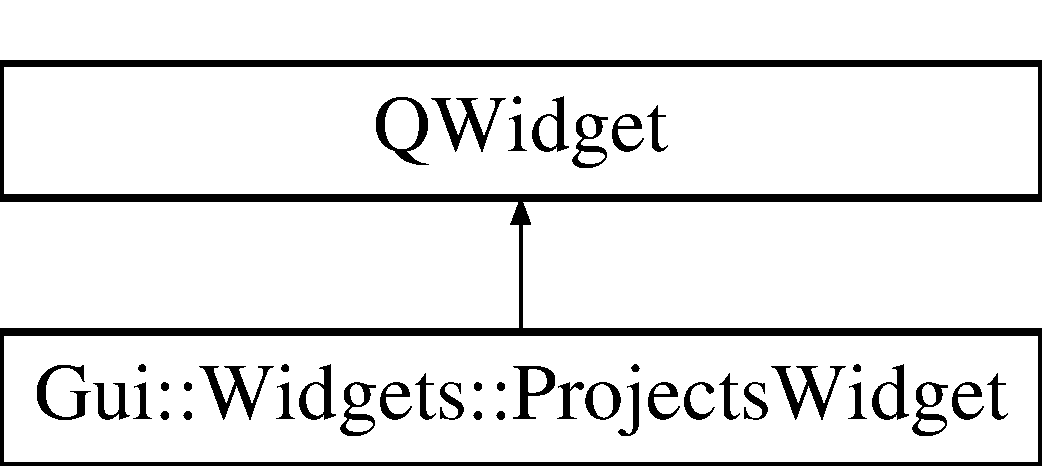
\includegraphics[height=2.000000cm]{dc/d8c/classGui_1_1Widgets_1_1ProjectsWidget}
\end{center}
\end{figure}
\subsection*{Public Slots}
\begin{DoxyCompactItemize}
\item 
\hypertarget{classGui_1_1Widgets_1_1ProjectsWidget_acd6cd65ef7bf569ce4e44436d2f8b4f4}{void \hyperlink{classGui_1_1Widgets_1_1ProjectsWidget_acd6cd65ef7bf569ce4e44436d2f8b4f4}{new\-Project} ()}\label{classGui_1_1Widgets_1_1ProjectsWidget_acd6cd65ef7bf569ce4e44436d2f8b4f4}

\begin{DoxyCompactList}\small\item\em \hyperlink{classGui_1_1Widgets_1_1ProjectsWidget_a25a20fde082c2698d7067d10e5795c0f}{Projects\-Widget\-::add\-Project} Event which sends a signal to add a new project. \end{DoxyCompactList}\item 
\hypertarget{classGui_1_1Widgets_1_1ProjectsWidget_a33284320194d2c20ac6a47ebaaa57ad4}{void \hyperlink{classGui_1_1Widgets_1_1ProjectsWidget_a33284320194d2c20ac6a47ebaaa57ad4}{edit\-Selected\-Project} ()}\label{classGui_1_1Widgets_1_1ProjectsWidget_a33284320194d2c20ac6a47ebaaa57ad4}

\begin{DoxyCompactList}\small\item\em \hyperlink{classGui_1_1Widgets_1_1ProjectsWidget_a33284320194d2c20ac6a47ebaaa57ad4}{Projects\-Widget\-::edit\-Selected\-Project} Event which sends a signal to edit the project selected. \end{DoxyCompactList}\item 
\hypertarget{classGui_1_1Widgets_1_1ProjectsWidget_a02d9111ae56ff401bc512fa218161d94}{void \hyperlink{classGui_1_1Widgets_1_1ProjectsWidget_a02d9111ae56ff401bc512fa218161d94}{remove\-Selected\-Project} ()}\label{classGui_1_1Widgets_1_1ProjectsWidget_a02d9111ae56ff401bc512fa218161d94}

\begin{DoxyCompactList}\small\item\em \hyperlink{classGui_1_1Widgets_1_1ProjectsWidget_a02d9111ae56ff401bc512fa218161d94}{Projects\-Widget\-::remove\-Selected\-Project} Event which sends a signal to remove the project selected. \end{DoxyCompactList}\item 
void \hyperlink{classGui_1_1Widgets_1_1ProjectsWidget_a3051880516e89826876afdf01fa6637a}{update\-Btn} (bool b)
\begin{DoxyCompactList}\small\item\em \hyperlink{classGui_1_1Widgets_1_1ProjectsWidget_a3051880516e89826876afdf01fa6637a}{Projects\-Widget\-::update\-Btn} Update the toolbar in tbl\-Projects. \end{DoxyCompactList}\end{DoxyCompactItemize}
\subsection*{Signals}
\begin{DoxyCompactItemize}
\item 
\hypertarget{classGui_1_1Widgets_1_1ProjectsWidget_a25a20fde082c2698d7067d10e5795c0f}{void \hyperlink{classGui_1_1Widgets_1_1ProjectsWidget_a25a20fde082c2698d7067d10e5795c0f}{add\-Project} ()}\label{classGui_1_1Widgets_1_1ProjectsWidget_a25a20fde082c2698d7067d10e5795c0f}

\begin{DoxyCompactList}\small\item\em \hyperlink{classGui_1_1Widgets_1_1ProjectsWidget_a25a20fde082c2698d7067d10e5795c0f}{Projects\-Widget\-::add\-Project} Add a new project to the current Customer. \end{DoxyCompactList}\item 
\hypertarget{classGui_1_1Widgets_1_1ProjectsWidget_a8a49da147544ffd78131af2b9289c9d0}{void \hyperlink{classGui_1_1Widgets_1_1ProjectsWidget_a8a49da147544ffd78131af2b9289c9d0}{edit\-Project} ()}\label{classGui_1_1Widgets_1_1ProjectsWidget_a8a49da147544ffd78131af2b9289c9d0}

\begin{DoxyCompactList}\small\item\em \hyperlink{classGui_1_1Widgets_1_1ProjectsWidget_a8a49da147544ffd78131af2b9289c9d0}{Projects\-Widget\-::edit\-Project} Edit the current Customer selected. \end{DoxyCompactList}\item 
\hypertarget{classGui_1_1Widgets_1_1ProjectsWidget_ac713b0c5c9afba988923fe3e29b405dc}{void \hyperlink{classGui_1_1Widgets_1_1ProjectsWidget_ac713b0c5c9afba988923fe3e29b405dc}{remove\-Project} ()}\label{classGui_1_1Widgets_1_1ProjectsWidget_ac713b0c5c9afba988923fe3e29b405dc}

\begin{DoxyCompactList}\small\item\em \hyperlink{classGui_1_1Widgets_1_1ProjectsWidget_ac713b0c5c9afba988923fe3e29b405dc}{Projects\-Widget\-::remove\-Project} Remove the current Customer selected. \end{DoxyCompactList}\end{DoxyCompactItemize}
\subsection*{Public Member Functions}
\begin{DoxyCompactItemize}
\item 
\hyperlink{classGui_1_1Widgets_1_1ProjectsWidget_a400712a956057c7233c396bffeb7a086}{Projects\-Widget} (Q\-Widget $\ast$parent=0)
\begin{DoxyCompactList}\small\item\em \hyperlink{classGui_1_1Widgets_1_1ProjectsWidget_a400712a956057c7233c396bffeb7a086}{Projects\-Widget\-::\-Projects\-Widget} Construct a \hyperlink{classGui_1_1Widgets_1_1ProjectsWidget}{Projects\-Widget}. \end{DoxyCompactList}\end{DoxyCompactItemize}


\subsection{Detailed Description}
The \hyperlink{classGui_1_1Widgets_1_1ProjectsWidget}{Projects\-Widget} class Actions on Project. 

\begin{DoxyAuthor}{Author}
Florent Berbie 
\end{DoxyAuthor}


\subsection{Constructor \& Destructor Documentation}
\hypertarget{classGui_1_1Widgets_1_1ProjectsWidget_a400712a956057c7233c396bffeb7a086}{\index{Gui\-::\-Widgets\-::\-Projects\-Widget@{Gui\-::\-Widgets\-::\-Projects\-Widget}!Projects\-Widget@{Projects\-Widget}}
\index{Projects\-Widget@{Projects\-Widget}!Gui::Widgets::ProjectsWidget@{Gui\-::\-Widgets\-::\-Projects\-Widget}}
\subsubsection[{Projects\-Widget}]{\setlength{\rightskip}{0pt plus 5cm}Gui\-::\-Widgets\-::\-Projects\-Widget\-::\-Projects\-Widget (
\begin{DoxyParamCaption}
\item[{Q\-Widget $\ast$}]{parent = {\ttfamily 0}}
\end{DoxyParamCaption}
)\hspace{0.3cm}{\ttfamily [explicit]}}}\label{classGui_1_1Widgets_1_1ProjectsWidget_a400712a956057c7233c396bffeb7a086}


\hyperlink{classGui_1_1Widgets_1_1ProjectsWidget_a400712a956057c7233c396bffeb7a086}{Projects\-Widget\-::\-Projects\-Widget} Construct a \hyperlink{classGui_1_1Widgets_1_1ProjectsWidget}{Projects\-Widget}. 


\begin{DoxyParams}{Parameters}
{\em parent} & \\
\hline
\end{DoxyParams}


\subsection{Member Function Documentation}
\hypertarget{classGui_1_1Widgets_1_1ProjectsWidget_a3051880516e89826876afdf01fa6637a}{\index{Gui\-::\-Widgets\-::\-Projects\-Widget@{Gui\-::\-Widgets\-::\-Projects\-Widget}!update\-Btn@{update\-Btn}}
\index{update\-Btn@{update\-Btn}!Gui::Widgets::ProjectsWidget@{Gui\-::\-Widgets\-::\-Projects\-Widget}}
\subsubsection[{update\-Btn}]{\setlength{\rightskip}{0pt plus 5cm}void Gui\-::\-Widgets\-::\-Projects\-Widget\-::update\-Btn (
\begin{DoxyParamCaption}
\item[{bool}]{b}
\end{DoxyParamCaption}
)\hspace{0.3cm}{\ttfamily [slot]}}}\label{classGui_1_1Widgets_1_1ProjectsWidget_a3051880516e89826876afdf01fa6637a}


\hyperlink{classGui_1_1Widgets_1_1ProjectsWidget_a3051880516e89826876afdf01fa6637a}{Projects\-Widget\-::update\-Btn} Update the toolbar in tbl\-Projects. 


\begin{DoxyParams}{Parameters}
{\em boolean} & if a row is selected \\
\hline
\end{DoxyParams}


The documentation for this class was generated from the following files\-:\begin{DoxyCompactItemize}
\item 
/home/travis/build/\-F\-A\-C\-T-\/\-Team/\-Fact\-Dev/src/gui/widgets/projectswidget.\-h\item 
/home/travis/build/\-F\-A\-C\-T-\/\-Team/\-Fact\-Dev/src/gui/widgets/projectswidget.\-cpp\end{DoxyCompactItemize}

\hypertarget{classGui_1_1Widgets_1_1RateWidget}{\section{Gui\-:\-:Widgets\-:\-:Rate\-Widget Class Reference}
\label{classGui_1_1Widgets_1_1RateWidget}\index{Gui\-::\-Widgets\-::\-Rate\-Widget@{Gui\-::\-Widgets\-::\-Rate\-Widget}}
}


Class for display Rate.  




{\ttfamily \#include $<$ratewidget.\-h$>$}

Inheritance diagram for Gui\-:\-:Widgets\-:\-:Rate\-Widget\-:\begin{figure}[H]
\begin{center}
\leavevmode
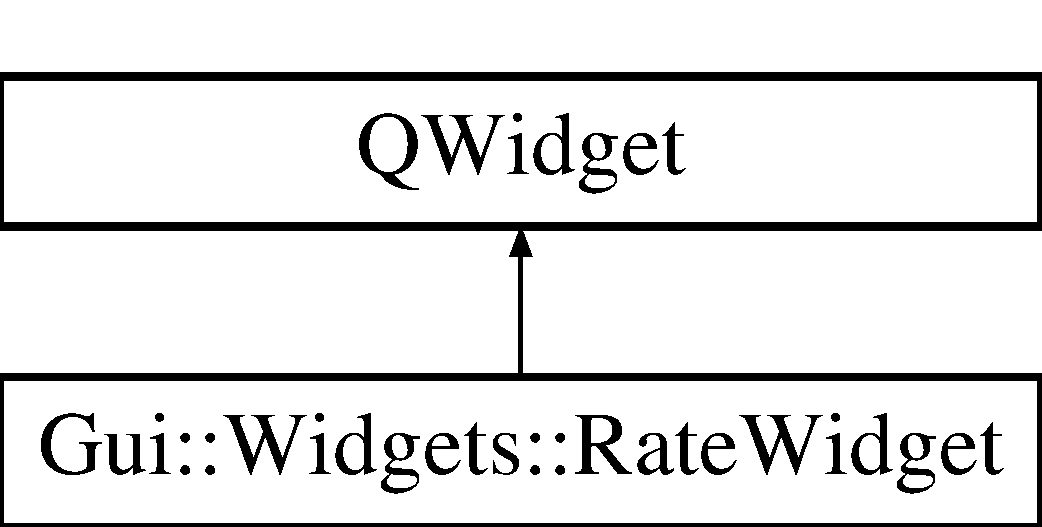
\includegraphics[height=2.000000cm]{d0/de2/classGui_1_1Widgets_1_1RateWidget}
\end{center}
\end{figure}
\subsection*{Public Slots}
\begin{DoxyCompactItemize}
\item 
void \hyperlink{classGui_1_1Widgets_1_1RateWidget_a6709f344452ce25d111e503bf8087582}{set\-Daily\-Rate} ()
\begin{DoxyCompactList}\small\item\em set\-Daily\-Rate Set a new value for the daily rate \end{DoxyCompactList}\item 
void \hyperlink{classGui_1_1Widgets_1_1RateWidget_a5c45d856fa577d87d6b9c2a4821fb804}{set\-Hourly\-Rate} ()
\begin{DoxyCompactList}\small\item\em set\-Hourly\-Rate Set a new value for the hourly rate \end{DoxyCompactList}\end{DoxyCompactItemize}
\subsection*{Public Member Functions}
\begin{DoxyCompactItemize}
\item 
\hyperlink{classGui_1_1Widgets_1_1RateWidget_a661ba8151fc842dcad246a7beb81de15}{Rate\-Widget} (Q\-Widget $\ast$parent=0)
\begin{DoxyCompactList}\small\item\em \hyperlink{classGui_1_1Widgets_1_1RateWidget_a661ba8151fc842dcad246a7beb81de15}{Rate\-Widget\-::\-Rate\-Widget} Construct a rate widget. \end{DoxyCompactList}\item 
\hypertarget{classGui_1_1Widgets_1_1RateWidget_aaad3463fdd580fb30af147bee194d986}{void \hyperlink{classGui_1_1Widgets_1_1RateWidget_aaad3463fdd580fb30af147bee194d986}{init\-Rate} ()}\label{classGui_1_1Widgets_1_1RateWidget_aaad3463fdd580fb30af147bee194d986}

\begin{DoxyCompactList}\small\item\em \hyperlink{classGui_1_1Widgets_1_1RateWidget_aaad3463fdd580fb30af147bee194d986}{Rate\-Widget\-::init\-Rate} Initialize the rate. \end{DoxyCompactList}\item 
void \hyperlink{classGui_1_1Widgets_1_1RateWidget_ae45a317c4472714c742b472b40c8028a}{set\-Widget\-Daily\-Rate\-Value} (double value)
\begin{DoxyCompactList}\small\item\em \hyperlink{classGui_1_1Widgets_1_1RateWidget_ae45a317c4472714c742b472b40c8028a}{Rate\-Widget\-::set\-Widget\-Daily\-Rate\-Value} Modify the {\itshape value} of the daily rate spin box component. \end{DoxyCompactList}\item 
double \hyperlink{classGui_1_1Widgets_1_1RateWidget_a2020dfe26413b0a940e6c9c9bf3e5aa6}{get\-Daily\-Rate} ()
\begin{DoxyCompactList}\small\item\em \hyperlink{classGui_1_1Widgets_1_1RateWidget_a2020dfe26413b0a940e6c9c9bf3e5aa6}{Rate\-Widget\-::get\-Daily\-Rate} Get the daily rate. \end{DoxyCompactList}\item 
double \hyperlink{classGui_1_1Widgets_1_1RateWidget_a710d062c9dfdb11c0b66174aa392e617}{get\-Hourly\-Rate} ()
\begin{DoxyCompactList}\small\item\em \hyperlink{classGui_1_1Widgets_1_1RateWidget_a710d062c9dfdb11c0b66174aa392e617}{Rate\-Widget\-::get\-Hourly\-Rate} Get the hourly rate. \end{DoxyCompactList}\item 
void \hyperlink{classGui_1_1Widgets_1_1RateWidget_a9d7eecd8f136accd39699ae209fb6edf}{set\-Widget\-Hourly\-Rate\-Value} (double value)
\begin{DoxyCompactList}\small\item\em \hyperlink{classGui_1_1Widgets_1_1RateWidget_a9d7eecd8f136accd39699ae209fb6edf}{Rate\-Widget\-::set\-Widget\-Hourly\-Rate\-Value} Modify the {\itshape value} of the hourly rate spin box component. \end{DoxyCompactList}\item 
\hypertarget{classGui_1_1Widgets_1_1RateWidget_ab5b8f371cee5a697470639f64e7856d6}{void \hyperlink{classGui_1_1Widgets_1_1RateWidget_ab5b8f371cee5a697470639f64e7856d6}{update\-Conversion\-Rate} ()}\label{classGui_1_1Widgets_1_1RateWidget_ab5b8f371cee5a697470639f64e7856d6}

\begin{DoxyCompactList}\small\item\em update\-Conversion\-Rate Update daily rate or hourly rate \end{DoxyCompactList}\end{DoxyCompactItemize}


\subsection{Detailed Description}
Class for display Rate. 

\begin{DoxyAuthor}{Author}
Florent Berbie 
\end{DoxyAuthor}


\subsection{Constructor \& Destructor Documentation}
\hypertarget{classGui_1_1Widgets_1_1RateWidget_a661ba8151fc842dcad246a7beb81de15}{\index{Gui\-::\-Widgets\-::\-Rate\-Widget@{Gui\-::\-Widgets\-::\-Rate\-Widget}!Rate\-Widget@{Rate\-Widget}}
\index{Rate\-Widget@{Rate\-Widget}!Gui::Widgets::RateWidget@{Gui\-::\-Widgets\-::\-Rate\-Widget}}
\subsubsection[{Rate\-Widget}]{\setlength{\rightskip}{0pt plus 5cm}Gui\-::\-Widgets\-::\-Rate\-Widget\-::\-Rate\-Widget (
\begin{DoxyParamCaption}
\item[{Q\-Widget $\ast$}]{parent = {\ttfamily 0}}
\end{DoxyParamCaption}
)\hspace{0.3cm}{\ttfamily [explicit]}}}\label{classGui_1_1Widgets_1_1RateWidget_a661ba8151fc842dcad246a7beb81de15}


\hyperlink{classGui_1_1Widgets_1_1RateWidget_a661ba8151fc842dcad246a7beb81de15}{Rate\-Widget\-::\-Rate\-Widget} Construct a rate widget. 


\begin{DoxyParams}{Parameters}
{\em parent} & The Q\-Widget parent \\
\hline
\end{DoxyParams}


\subsection{Member Function Documentation}
\hypertarget{classGui_1_1Widgets_1_1RateWidget_a2020dfe26413b0a940e6c9c9bf3e5aa6}{\index{Gui\-::\-Widgets\-::\-Rate\-Widget@{Gui\-::\-Widgets\-::\-Rate\-Widget}!get\-Daily\-Rate@{get\-Daily\-Rate}}
\index{get\-Daily\-Rate@{get\-Daily\-Rate}!Gui::Widgets::RateWidget@{Gui\-::\-Widgets\-::\-Rate\-Widget}}
\subsubsection[{get\-Daily\-Rate}]{\setlength{\rightskip}{0pt plus 5cm}double Gui\-::\-Widgets\-::\-Rate\-Widget\-::get\-Daily\-Rate (
\begin{DoxyParamCaption}
{}
\end{DoxyParamCaption}
)}}\label{classGui_1_1Widgets_1_1RateWidget_a2020dfe26413b0a940e6c9c9bf3e5aa6}


\hyperlink{classGui_1_1Widgets_1_1RateWidget_a2020dfe26413b0a940e6c9c9bf3e5aa6}{Rate\-Widget\-::get\-Daily\-Rate} Get the daily rate. 

\begin{DoxyReturn}{Returns}
The daily rate 
\end{DoxyReturn}
\hypertarget{classGui_1_1Widgets_1_1RateWidget_a710d062c9dfdb11c0b66174aa392e617}{\index{Gui\-::\-Widgets\-::\-Rate\-Widget@{Gui\-::\-Widgets\-::\-Rate\-Widget}!get\-Hourly\-Rate@{get\-Hourly\-Rate}}
\index{get\-Hourly\-Rate@{get\-Hourly\-Rate}!Gui::Widgets::RateWidget@{Gui\-::\-Widgets\-::\-Rate\-Widget}}
\subsubsection[{get\-Hourly\-Rate}]{\setlength{\rightskip}{0pt plus 5cm}double Gui\-::\-Widgets\-::\-Rate\-Widget\-::get\-Hourly\-Rate (
\begin{DoxyParamCaption}
{}
\end{DoxyParamCaption}
)}}\label{classGui_1_1Widgets_1_1RateWidget_a710d062c9dfdb11c0b66174aa392e617}


\hyperlink{classGui_1_1Widgets_1_1RateWidget_a710d062c9dfdb11c0b66174aa392e617}{Rate\-Widget\-::get\-Hourly\-Rate} Get the hourly rate. 

\begin{DoxyReturn}{Returns}
The hourly rate 
\end{DoxyReturn}
\hypertarget{classGui_1_1Widgets_1_1RateWidget_a6709f344452ce25d111e503bf8087582}{\index{Gui\-::\-Widgets\-::\-Rate\-Widget@{Gui\-::\-Widgets\-::\-Rate\-Widget}!set\-Daily\-Rate@{set\-Daily\-Rate}}
\index{set\-Daily\-Rate@{set\-Daily\-Rate}!Gui::Widgets::RateWidget@{Gui\-::\-Widgets\-::\-Rate\-Widget}}
\subsubsection[{set\-Daily\-Rate}]{\setlength{\rightskip}{0pt plus 5cm}void Gui\-::\-Widgets\-::\-Rate\-Widget\-::set\-Daily\-Rate (
\begin{DoxyParamCaption}
{}
\end{DoxyParamCaption}
)\hspace{0.3cm}{\ttfamily [slot]}}}\label{classGui_1_1Widgets_1_1RateWidget_a6709f344452ce25d111e503bf8087582}


set\-Daily\-Rate Set a new value for the daily rate 


\begin{DoxyParams}{Parameters}
{\em daily\-Rate} & The new daily rate \\
\hline
\end{DoxyParams}
\hypertarget{classGui_1_1Widgets_1_1RateWidget_a5c45d856fa577d87d6b9c2a4821fb804}{\index{Gui\-::\-Widgets\-::\-Rate\-Widget@{Gui\-::\-Widgets\-::\-Rate\-Widget}!set\-Hourly\-Rate@{set\-Hourly\-Rate}}
\index{set\-Hourly\-Rate@{set\-Hourly\-Rate}!Gui::Widgets::RateWidget@{Gui\-::\-Widgets\-::\-Rate\-Widget}}
\subsubsection[{set\-Hourly\-Rate}]{\setlength{\rightskip}{0pt plus 5cm}void Gui\-::\-Widgets\-::\-Rate\-Widget\-::set\-Hourly\-Rate (
\begin{DoxyParamCaption}
{}
\end{DoxyParamCaption}
)\hspace{0.3cm}{\ttfamily [slot]}}}\label{classGui_1_1Widgets_1_1RateWidget_a5c45d856fa577d87d6b9c2a4821fb804}


set\-Hourly\-Rate Set a new value for the hourly rate 


\begin{DoxyParams}{Parameters}
{\em hourly\-Rate} & The new hourly rate \\
\hline
\end{DoxyParams}
\hypertarget{classGui_1_1Widgets_1_1RateWidget_ae45a317c4472714c742b472b40c8028a}{\index{Gui\-::\-Widgets\-::\-Rate\-Widget@{Gui\-::\-Widgets\-::\-Rate\-Widget}!set\-Widget\-Daily\-Rate\-Value@{set\-Widget\-Daily\-Rate\-Value}}
\index{set\-Widget\-Daily\-Rate\-Value@{set\-Widget\-Daily\-Rate\-Value}!Gui::Widgets::RateWidget@{Gui\-::\-Widgets\-::\-Rate\-Widget}}
\subsubsection[{set\-Widget\-Daily\-Rate\-Value}]{\setlength{\rightskip}{0pt plus 5cm}void Gui\-::\-Widgets\-::\-Rate\-Widget\-::set\-Widget\-Daily\-Rate\-Value (
\begin{DoxyParamCaption}
\item[{double}]{value}
\end{DoxyParamCaption}
)}}\label{classGui_1_1Widgets_1_1RateWidget_ae45a317c4472714c742b472b40c8028a}


\hyperlink{classGui_1_1Widgets_1_1RateWidget_ae45a317c4472714c742b472b40c8028a}{Rate\-Widget\-::set\-Widget\-Daily\-Rate\-Value} Modify the {\itshape value} of the daily rate spin box component. 


\begin{DoxyParams}{Parameters}
{\em value} & New Value \\
\hline
\end{DoxyParams}
\hypertarget{classGui_1_1Widgets_1_1RateWidget_a9d7eecd8f136accd39699ae209fb6edf}{\index{Gui\-::\-Widgets\-::\-Rate\-Widget@{Gui\-::\-Widgets\-::\-Rate\-Widget}!set\-Widget\-Hourly\-Rate\-Value@{set\-Widget\-Hourly\-Rate\-Value}}
\index{set\-Widget\-Hourly\-Rate\-Value@{set\-Widget\-Hourly\-Rate\-Value}!Gui::Widgets::RateWidget@{Gui\-::\-Widgets\-::\-Rate\-Widget}}
\subsubsection[{set\-Widget\-Hourly\-Rate\-Value}]{\setlength{\rightskip}{0pt plus 5cm}void Gui\-::\-Widgets\-::\-Rate\-Widget\-::set\-Widget\-Hourly\-Rate\-Value (
\begin{DoxyParamCaption}
\item[{double}]{value}
\end{DoxyParamCaption}
)}}\label{classGui_1_1Widgets_1_1RateWidget_a9d7eecd8f136accd39699ae209fb6edf}


\hyperlink{classGui_1_1Widgets_1_1RateWidget_a9d7eecd8f136accd39699ae209fb6edf}{Rate\-Widget\-::set\-Widget\-Hourly\-Rate\-Value} Modify the {\itshape value} of the hourly rate spin box component. 


\begin{DoxyParams}{Parameters}
{\em value} & New value \\
\hline
\end{DoxyParams}


The documentation for this class was generated from the following files\-:\begin{DoxyCompactItemize}
\item 
/home/florent/\-Documents/\-Projet\-\_\-\-S8/\-Fact\-Dev/src/gui/widgets/ratewidget.\-h\item 
/home/florent/\-Documents/\-Projet\-\_\-\-S8/\-Fact\-Dev/src/gui/widgets/ratewidget.\-cpp\end{DoxyCompactItemize}

\hypertarget{classModels_1_1Search}{}\section{Models\+:\+:Search Class Reference}
\label{classModels_1_1Search}\index{Models\+::\+Search@{Models\+::\+Search}}


The \hyperlink{classModels_1_1Search}{Search} class.  




{\ttfamily \#include $<$search.\+h$>$}

\subsection*{Public Member Functions}
\begin{DoxyCompactItemize}
\item 
\hypertarget{classModels_1_1Search_a05ea0037161dce5dde6876afa384d71f}{}\hyperlink{classModels_1_1Search_a05ea0037161dce5dde6876afa384d71f}{Search} ()\label{classModels_1_1Search_a05ea0037161dce5dde6876afa384d71f}

\begin{DoxyCompactList}\small\item\em \hyperlink{classModels_1_1Search_a05ea0037161dce5dde6876afa384d71f}{Search\+::\+Search} Construct a search. \end{DoxyCompactList}\item 
\hypertarget{classModels_1_1Search_a6b51a9a47bfc35addb8204ff89afefe3}{}\hyperlink{classModels_1_1Search_a6b51a9a47bfc35addb8204ff89afefe3}{$\sim$\+Search} ()\label{classModels_1_1Search_a6b51a9a47bfc35addb8204ff89afefe3}

\begin{DoxyCompactList}\small\item\em \hyperlink{classModels_1_1Search_a05ea0037161dce5dde6876afa384d71f}{Search\+::\+Search} Destruct a search. \end{DoxyCompactList}\item 
Q\+String \hyperlink{classModels_1_1Search_ab3ec88b48f6b404f8027dcbfce1495c6}{get\+Filter} ()
\begin{DoxyCompactList}\small\item\em \hyperlink{classModels_1_1Search_ab3ec88b48f6b404f8027dcbfce1495c6}{Search\+::get\+Filter} Return the search filter. \end{DoxyCompactList}\item 
void \hyperlink{classModels_1_1Search_a63afd22af898b54b405be45a8a1ff843}{filter\+On\+Varchar\+Elements} (Q\+String \&filter, const Q\+String\+List list, Q\+String element)
\begin{DoxyCompactList}\small\item\em \hyperlink{classModels_1_1Search_a63afd22af898b54b405be45a8a1ff843}{Search\+::filter\+On\+Varchar\+Elements} \hyperlink{classModels_1_1Search}{Search}, for each word of the {\itshape list} from the {\itshape filter}, if it corresponds to the {\itshape element} in the database. \end{DoxyCompactList}\item 
void \hyperlink{classModels_1_1Search_ab7c6fc3cf9062848c118ab7e8380726c}{filter\+On\+Number\+Elements} (Q\+String \&filter, const Q\+String\+List list, Q\+String element)
\begin{DoxyCompactList}\small\item\em \hyperlink{classModels_1_1Search_ab7c6fc3cf9062848c118ab7e8380726c}{Search\+::filter\+On\+Number\+Elements} \hyperlink{classModels_1_1Search}{Search}, for each number of the {\itshape list} from the {\itshape filter}, if it corresponds to the {\itshape element} in the database. \end{DoxyCompactList}\item 
void \hyperlink{classModels_1_1Search_af5e7f802c53a735915193fd596d45f07}{filter\+On\+Company} (Q\+String \&filter, const Q\+String\+List list)
\begin{DoxyCompactList}\small\item\em \hyperlink{classModels_1_1Search_af5e7f802c53a735915193fd596d45f07}{Search\+::filter\+On\+Company} \hyperlink{classModels_1_1Search}{Search} all companies contained in the {\itshape list} of the {\itshape filter} \end{DoxyCompactList}\item 
void \hyperlink{classModels_1_1Search_a27536d8a999a32164e1ac90bf9d24906}{filter\+On\+Referent\+Lastname} (Q\+String \&filter, const Q\+String\+List list)
\begin{DoxyCompactList}\small\item\em \hyperlink{classModels_1_1Search_a27536d8a999a32164e1ac90bf9d24906}{Search\+::filter\+On\+Referent\+Lastname} \hyperlink{classModels_1_1Search}{Search} all referents last name contained in the {\itshape list} of the {\itshape filter} \end{DoxyCompactList}\item 
void \hyperlink{classModels_1_1Search_a4f5672fa4dc52e3ea7bda9b4c654147f}{filter\+On\+Projects} (Q\+String \&filter, const Q\+String\+List list)
\begin{DoxyCompactList}\small\item\em \hyperlink{classModels_1_1Search_a4f5672fa4dc52e3ea7bda9b4c654147f}{Search\+::filter\+On\+Projects} \hyperlink{classModels_1_1Search}{Search} all projects contained in the {\itshape list} of the {\itshape filter} \end{DoxyCompactList}\item 
void \hyperlink{classModels_1_1Search_acb948c15a52305c29cf4c5b9489e9f18}{filter\+On\+Contributories} (Q\+String \&filter, const Q\+String\+List list)
\begin{DoxyCompactList}\small\item\em \hyperlink{classModels_1_1Search_acb948c15a52305c29cf4c5b9489e9f18}{Search\+::filter\+On\+Contributories} \hyperlink{classModels_1_1Search}{Search} all contributories contained in the {\itshape list} of the {\itshape filter} \end{DoxyCompactList}\item 
void \hyperlink{classModels_1_1Search_ad80f840390720ad3239aa0fc87e483fc}{filter\+On\+Bills\+Or\+Quotes} (Q\+String \&filter, const Q\+String\+List list)
\begin{DoxyCompactList}\small\item\em \hyperlink{classModels_1_1Search_ad80f840390720ad3239aa0fc87e483fc}{Search\+::filter\+On\+Bills\+Or\+Quotes} \hyperlink{classModels_1_1Search}{Search} all bills or quotes which are contained in the {\itshape list} of the {\itshape filter} \end{DoxyCompactList}\item 
void \hyperlink{classModels_1_1Search_af92c03f00f81edeaf5a209d7b830be3a}{filter\+On\+Customers\+Without\+Project} (Q\+String \&filter, const Q\+String\+List list)
\begin{DoxyCompactList}\small\item\em \hyperlink{classModels_1_1Search_af92c03f00f81edeaf5a209d7b830be3a}{Search\+::filter\+On\+Customers\+Without\+Project} \hyperlink{classModels_1_1Search}{Search} all customers which are contained in the {\itshape list} of the {\itshape filter} \end{DoxyCompactList}\item 
bool \hyperlink{classModels_1_1Search_ad38428f4aa81ba5951f82e0fcb92779c}{get\+Search\+In\+Companies} () const 
\begin{DoxyCompactList}\small\item\em \hyperlink{classModels_1_1Search_ad38428f4aa81ba5951f82e0fcb92779c}{Search\+::get\+Search\+In\+Companies} Return if we search a company. \end{DoxyCompactList}\item 
void \hyperlink{classModels_1_1Search_a3a630b2b2a48fb013b4c8cb9756fa813}{set\+Search\+In\+Companies} (bool search\+In\+Companies)
\begin{DoxyCompactList}\small\item\em \hyperlink{classModels_1_1Search_a3a630b2b2a48fb013b4c8cb9756fa813}{Search\+::set\+Search\+In\+Companies} Modify the filter of companies search. \end{DoxyCompactList}\item 
bool \hyperlink{classModels_1_1Search_aa415bcd966fef7bcd1cd5bd3373d57f6}{get\+Search\+In\+Referent\+Lastname} () const 
\begin{DoxyCompactList}\small\item\em \hyperlink{classModels_1_1Search_aa415bcd966fef7bcd1cd5bd3373d57f6}{Search\+::get\+Search\+In\+Referent\+Lastname} Return if we search a Last name referent. \end{DoxyCompactList}\item 
void \hyperlink{classModels_1_1Search_a4a897b3e19a0a6ce9e37ae1a73b39240}{set\+Search\+In\+Referent\+Lastname} (bool search\+In\+Referent\+Lastname)
\begin{DoxyCompactList}\small\item\em \hyperlink{classModels_1_1Search_a4a897b3e19a0a6ce9e37ae1a73b39240}{Search\+::set\+Search\+In\+Referent\+Lastname} Modify the filter of referents last name search. \end{DoxyCompactList}\item 
bool \hyperlink{classModels_1_1Search_a6c8f401bb696db96cc57a635d46910dd}{get\+Search\+In\+Projects} () const 
\begin{DoxyCompactList}\small\item\em \hyperlink{classModels_1_1Search_a6c8f401bb696db96cc57a635d46910dd}{Search\+::get\+Search\+In\+Projects} Return T\+R\+U\+E if it exists one or more projets in database. \end{DoxyCompactList}\item 
void \hyperlink{classModels_1_1Search_ab84375da3e302c7a871b4ced1c8d69c3}{set\+Search\+In\+Projects} (bool search\+In\+Projects)
\begin{DoxyCompactList}\small\item\em \hyperlink{classModels_1_1Search_ab84375da3e302c7a871b4ced1c8d69c3}{Search\+::set\+Search\+In\+Projects} Modify the filter of projects search. \end{DoxyCompactList}\item 
bool \hyperlink{classModels_1_1Search_ab799572f484cc01a515b36ea3723ee06}{search\+In\+Contributories} () const 
\begin{DoxyCompactList}\small\item\em Search\+::get\+Search\+In\+Contributories Return T\+R\+U\+E if it exists one or more projets in database. \end{DoxyCompactList}\item 
void \hyperlink{classModels_1_1Search_af6305e66a5ca5ad5ba29b15397821e58}{set\+Search\+In\+Contributories} (bool \hyperlink{classModels_1_1Search_ab799572f484cc01a515b36ea3723ee06}{search\+In\+Contributories})
\begin{DoxyCompactList}\small\item\em \hyperlink{classModels_1_1Search_af6305e66a5ca5ad5ba29b15397821e58}{Search\+::set\+Search\+In\+Contributories} Modify the filter of contributories search. \end{DoxyCompactList}\item 
bool \hyperlink{classModels_1_1Search_adf4525d5961793999c191e010a58bb56}{get\+Search\+In\+Bills\+Quotes} () const 
\begin{DoxyCompactList}\small\item\em Search\+::search\+In\+Bills\+Quotes Return T\+R\+U\+E if it exists one or more bills or quotes in database. \end{DoxyCompactList}\item 
void \hyperlink{classModels_1_1Search_a64f82cec524c9bb737e2758445288b43}{set\+Search\+In\+Bills\+Quotes} (bool search\+In\+Bills\+Quotes)
\begin{DoxyCompactList}\small\item\em \hyperlink{classModels_1_1Search_a64f82cec524c9bb737e2758445288b43}{Search\+::set\+Search\+In\+Bills\+Quotes} Modify the filter of bills and quotes search. \end{DoxyCompactList}\item 
bool \hyperlink{classModels_1_1Search_a2f5ee925709a654cedef85732e448438}{get\+Group\+Filter} () const 
\begin{DoxyCompactList}\small\item\em \hyperlink{classModels_1_1Search_a2f5ee925709a654cedef85732e448438}{Search\+::get\+Group\+Filter} Return if the filter is actived. \end{DoxyCompactList}\item 
void \hyperlink{classModels_1_1Search_a5feb06679973719e31007e659c08cc06}{set\+Group\+Filter} (bool \hyperlink{classModels_1_1Search_a2f5ee925709a654cedef85732e448438}{get\+Group\+Filter})
\begin{DoxyCompactList}\small\item\em \hyperlink{classModels_1_1Search_a5feb06679973719e31007e659c08cc06}{Search\+::set\+Group\+Filter} Modify if we active search filter. \end{DoxyCompactList}\item 
Q\+String \hyperlink{classModels_1_1Search_a30d4355f72278e6e466dc64208947f8b}{get\+Text} () const 
\begin{DoxyCompactList}\small\item\em \hyperlink{classModels_1_1Search_a30d4355f72278e6e466dc64208947f8b}{Search\+::get\+Text} Return sql portion of filter. \end{DoxyCompactList}\item 
void \hyperlink{classModels_1_1Search_a1bd00e3da5d5e10b4bec6579fb1c8bfa}{set\+Text} (const Q\+String \&\hyperlink{classModels_1_1Search_a30d4355f72278e6e466dc64208947f8b}{get\+Text})
\begin{DoxyCompactList}\small\item\em \hyperlink{classModels_1_1Search_a1bd00e3da5d5e10b4bec6579fb1c8bfa}{Search\+::set\+Text} Modify sql portion. \end{DoxyCompactList}\end{DoxyCompactItemize}


\subsection{Detailed Description}
The \hyperlink{classModels_1_1Search}{Search} class. 

\begin{DoxyAuthor}{Author}
Antoine de Roquemaurel 

Florent Berbie 
\end{DoxyAuthor}


\subsection{Member Function Documentation}
\hypertarget{classModels_1_1Search_ad80f840390720ad3239aa0fc87e483fc}{}\index{Models\+::\+Search@{Models\+::\+Search}!filter\+On\+Bills\+Or\+Quotes@{filter\+On\+Bills\+Or\+Quotes}}
\index{filter\+On\+Bills\+Or\+Quotes@{filter\+On\+Bills\+Or\+Quotes}!Models\+::\+Search@{Models\+::\+Search}}
\subsubsection[{filter\+On\+Bills\+Or\+Quotes}]{\setlength{\rightskip}{0pt plus 5cm}void Models\+::\+Search\+::filter\+On\+Bills\+Or\+Quotes (
\begin{DoxyParamCaption}
\item[{Q\+String \&}]{filter, }
\item[{const Q\+String\+List}]{list}
\end{DoxyParamCaption}
)}\label{classModels_1_1Search_ad80f840390720ad3239aa0fc87e483fc}


\hyperlink{classModels_1_1Search_ad80f840390720ad3239aa0fc87e483fc}{Search\+::filter\+On\+Bills\+Or\+Quotes} \hyperlink{classModels_1_1Search}{Search} all bills or quotes which are contained in the {\itshape list} of the {\itshape filter} 


\begin{DoxyParams}{Parameters}
{\em filter} & Text inputed in searchbar \\
\hline
{\em list} & List of bills or quotes \\
\hline
\end{DoxyParams}
\hypertarget{classModels_1_1Search_af5e7f802c53a735915193fd596d45f07}{}\index{Models\+::\+Search@{Models\+::\+Search}!filter\+On\+Company@{filter\+On\+Company}}
\index{filter\+On\+Company@{filter\+On\+Company}!Models\+::\+Search@{Models\+::\+Search}}
\subsubsection[{filter\+On\+Company}]{\setlength{\rightskip}{0pt plus 5cm}void Models\+::\+Search\+::filter\+On\+Company (
\begin{DoxyParamCaption}
\item[{Q\+String \&}]{filter, }
\item[{const Q\+String\+List}]{list}
\end{DoxyParamCaption}
)}\label{classModels_1_1Search_af5e7f802c53a735915193fd596d45f07}


\hyperlink{classModels_1_1Search_af5e7f802c53a735915193fd596d45f07}{Search\+::filter\+On\+Company} \hyperlink{classModels_1_1Search}{Search} all companies contained in the {\itshape list} of the {\itshape filter} 


\begin{DoxyParams}{Parameters}
{\em filter} & Text inputed in searchbar \\
\hline
{\em list} & List of companies \\
\hline
\end{DoxyParams}
\hypertarget{classModels_1_1Search_acb948c15a52305c29cf4c5b9489e9f18}{}\index{Models\+::\+Search@{Models\+::\+Search}!filter\+On\+Contributories@{filter\+On\+Contributories}}
\index{filter\+On\+Contributories@{filter\+On\+Contributories}!Models\+::\+Search@{Models\+::\+Search}}
\subsubsection[{filter\+On\+Contributories}]{\setlength{\rightskip}{0pt plus 5cm}void Models\+::\+Search\+::filter\+On\+Contributories (
\begin{DoxyParamCaption}
\item[{Q\+String \&}]{filter, }
\item[{const Q\+String\+List}]{list}
\end{DoxyParamCaption}
)}\label{classModels_1_1Search_acb948c15a52305c29cf4c5b9489e9f18}


\hyperlink{classModels_1_1Search_acb948c15a52305c29cf4c5b9489e9f18}{Search\+::filter\+On\+Contributories} \hyperlink{classModels_1_1Search}{Search} all contributories contained in the {\itshape list} of the {\itshape filter} 


\begin{DoxyParams}{Parameters}
{\em filter} & Text inputed in searchbar \\
\hline
{\em list} & List of contributories \\
\hline
\end{DoxyParams}
\hypertarget{classModels_1_1Search_af92c03f00f81edeaf5a209d7b830be3a}{}\index{Models\+::\+Search@{Models\+::\+Search}!filter\+On\+Customers\+Without\+Project@{filter\+On\+Customers\+Without\+Project}}
\index{filter\+On\+Customers\+Without\+Project@{filter\+On\+Customers\+Without\+Project}!Models\+::\+Search@{Models\+::\+Search}}
\subsubsection[{filter\+On\+Customers\+Without\+Project}]{\setlength{\rightskip}{0pt plus 5cm}void Models\+::\+Search\+::filter\+On\+Customers\+Without\+Project (
\begin{DoxyParamCaption}
\item[{Q\+String \&}]{filter, }
\item[{const Q\+String\+List}]{list}
\end{DoxyParamCaption}
)}\label{classModels_1_1Search_af92c03f00f81edeaf5a209d7b830be3a}


\hyperlink{classModels_1_1Search_af92c03f00f81edeaf5a209d7b830be3a}{Search\+::filter\+On\+Customers\+Without\+Project} \hyperlink{classModels_1_1Search}{Search} all customers which are contained in the {\itshape list} of the {\itshape filter} 


\begin{DoxyParams}{Parameters}
{\em filter} & Text inputed in searchbar \\
\hline
{\em list} & List of bills or quotes \\
\hline
\end{DoxyParams}
\hypertarget{classModels_1_1Search_ab7c6fc3cf9062848c118ab7e8380726c}{}\index{Models\+::\+Search@{Models\+::\+Search}!filter\+On\+Number\+Elements@{filter\+On\+Number\+Elements}}
\index{filter\+On\+Number\+Elements@{filter\+On\+Number\+Elements}!Models\+::\+Search@{Models\+::\+Search}}
\subsubsection[{filter\+On\+Number\+Elements}]{\setlength{\rightskip}{0pt plus 5cm}void Models\+::\+Search\+::filter\+On\+Number\+Elements (
\begin{DoxyParamCaption}
\item[{Q\+String \&}]{filter, }
\item[{const Q\+String\+List}]{list, }
\item[{Q\+String}]{element}
\end{DoxyParamCaption}
)}\label{classModels_1_1Search_ab7c6fc3cf9062848c118ab7e8380726c}


\hyperlink{classModels_1_1Search_ab7c6fc3cf9062848c118ab7e8380726c}{Search\+::filter\+On\+Number\+Elements} \hyperlink{classModels_1_1Search}{Search}, for each number of the {\itshape list} from the {\itshape filter}, if it corresponds to the {\itshape element} in the database. 


\begin{DoxyParams}{Parameters}
{\em filter} & Text inputed in the searchbar \\
\hline
{\em list} & List of numbers from the {\itshape filter} \\
\hline
{\em element} & Attribute name into the database \\
\hline
\end{DoxyParams}
\hypertarget{classModels_1_1Search_a4f5672fa4dc52e3ea7bda9b4c654147f}{}\index{Models\+::\+Search@{Models\+::\+Search}!filter\+On\+Projects@{filter\+On\+Projects}}
\index{filter\+On\+Projects@{filter\+On\+Projects}!Models\+::\+Search@{Models\+::\+Search}}
\subsubsection[{filter\+On\+Projects}]{\setlength{\rightskip}{0pt plus 5cm}void Models\+::\+Search\+::filter\+On\+Projects (
\begin{DoxyParamCaption}
\item[{Q\+String \&}]{filter, }
\item[{const Q\+String\+List}]{list}
\end{DoxyParamCaption}
)}\label{classModels_1_1Search_a4f5672fa4dc52e3ea7bda9b4c654147f}


\hyperlink{classModels_1_1Search_a4f5672fa4dc52e3ea7bda9b4c654147f}{Search\+::filter\+On\+Projects} \hyperlink{classModels_1_1Search}{Search} all projects contained in the {\itshape list} of the {\itshape filter} 


\begin{DoxyParams}{Parameters}
{\em filter} & Text inputed in searchbar \\
\hline
{\em list} & List of projects \\
\hline
\end{DoxyParams}
\hypertarget{classModels_1_1Search_a27536d8a999a32164e1ac90bf9d24906}{}\index{Models\+::\+Search@{Models\+::\+Search}!filter\+On\+Referent\+Lastname@{filter\+On\+Referent\+Lastname}}
\index{filter\+On\+Referent\+Lastname@{filter\+On\+Referent\+Lastname}!Models\+::\+Search@{Models\+::\+Search}}
\subsubsection[{filter\+On\+Referent\+Lastname}]{\setlength{\rightskip}{0pt plus 5cm}void Models\+::\+Search\+::filter\+On\+Referent\+Lastname (
\begin{DoxyParamCaption}
\item[{Q\+String \&}]{filter, }
\item[{const Q\+String\+List}]{list}
\end{DoxyParamCaption}
)}\label{classModels_1_1Search_a27536d8a999a32164e1ac90bf9d24906}


\hyperlink{classModels_1_1Search_a27536d8a999a32164e1ac90bf9d24906}{Search\+::filter\+On\+Referent\+Lastname} \hyperlink{classModels_1_1Search}{Search} all referents last name contained in the {\itshape list} of the {\itshape filter} 


\begin{DoxyParams}{Parameters}
{\em filter} & Text inputed in searchbar \\
\hline
{\em list} & List of referent last name \\
\hline
\end{DoxyParams}
\hypertarget{classModels_1_1Search_a63afd22af898b54b405be45a8a1ff843}{}\index{Models\+::\+Search@{Models\+::\+Search}!filter\+On\+Varchar\+Elements@{filter\+On\+Varchar\+Elements}}
\index{filter\+On\+Varchar\+Elements@{filter\+On\+Varchar\+Elements}!Models\+::\+Search@{Models\+::\+Search}}
\subsubsection[{filter\+On\+Varchar\+Elements}]{\setlength{\rightskip}{0pt plus 5cm}void Models\+::\+Search\+::filter\+On\+Varchar\+Elements (
\begin{DoxyParamCaption}
\item[{Q\+String \&}]{filter, }
\item[{const Q\+String\+List}]{list, }
\item[{Q\+String}]{element}
\end{DoxyParamCaption}
)}\label{classModels_1_1Search_a63afd22af898b54b405be45a8a1ff843}


\hyperlink{classModels_1_1Search_a63afd22af898b54b405be45a8a1ff843}{Search\+::filter\+On\+Varchar\+Elements} \hyperlink{classModels_1_1Search}{Search}, for each word of the {\itshape list} from the {\itshape filter}, if it corresponds to the {\itshape element} in the database. 


\begin{DoxyParams}{Parameters}
{\em filter} & Text inputed in the searchbar \\
\hline
{\em list} & List of words from the {\itshape filter} \\
\hline
{\em element} & Attribute name into the database \\
\hline
\end{DoxyParams}
\hypertarget{classModels_1_1Search_ab3ec88b48f6b404f8027dcbfce1495c6}{}\index{Models\+::\+Search@{Models\+::\+Search}!get\+Filter@{get\+Filter}}
\index{get\+Filter@{get\+Filter}!Models\+::\+Search@{Models\+::\+Search}}
\subsubsection[{get\+Filter}]{\setlength{\rightskip}{0pt plus 5cm}Q\+String Models\+::\+Search\+::get\+Filter (
\begin{DoxyParamCaption}
{}
\end{DoxyParamCaption}
)}\label{classModels_1_1Search_ab3ec88b48f6b404f8027dcbfce1495c6}


\hyperlink{classModels_1_1Search_ab3ec88b48f6b404f8027dcbfce1495c6}{Search\+::get\+Filter} Return the search filter. 

\begin{DoxyReturn}{Returns}
filter selected (sql portion) 
\end{DoxyReturn}
\hypertarget{classModels_1_1Search_a2f5ee925709a654cedef85732e448438}{}\index{Models\+::\+Search@{Models\+::\+Search}!get\+Group\+Filter@{get\+Group\+Filter}}
\index{get\+Group\+Filter@{get\+Group\+Filter}!Models\+::\+Search@{Models\+::\+Search}}
\subsubsection[{get\+Group\+Filter}]{\setlength{\rightskip}{0pt plus 5cm}bool Models\+::\+Search\+::get\+Group\+Filter (
\begin{DoxyParamCaption}
{}
\end{DoxyParamCaption}
) const}\label{classModels_1_1Search_a2f5ee925709a654cedef85732e448438}


\hyperlink{classModels_1_1Search_a2f5ee925709a654cedef85732e448438}{Search\+::get\+Group\+Filter} Return if the filter is actived. 

\begin{DoxyReturn}{Returns}
boolean if search filter is actived 
\end{DoxyReturn}
\hypertarget{classModels_1_1Search_adf4525d5961793999c191e010a58bb56}{}\index{Models\+::\+Search@{Models\+::\+Search}!get\+Search\+In\+Bills\+Quotes@{get\+Search\+In\+Bills\+Quotes}}
\index{get\+Search\+In\+Bills\+Quotes@{get\+Search\+In\+Bills\+Quotes}!Models\+::\+Search@{Models\+::\+Search}}
\subsubsection[{get\+Search\+In\+Bills\+Quotes}]{\setlength{\rightskip}{0pt plus 5cm}bool Models\+::\+Search\+::get\+Search\+In\+Bills\+Quotes (
\begin{DoxyParamCaption}
{}
\end{DoxyParamCaption}
) const}\label{classModels_1_1Search_adf4525d5961793999c191e010a58bb56}


Search\+::search\+In\+Bills\+Quotes Return T\+R\+U\+E if it exists one or more bills or quotes in database. 

\begin{DoxyReturn}{Returns}
boolean if bills or quotes are existing 
\end{DoxyReturn}
\hypertarget{classModels_1_1Search_ad38428f4aa81ba5951f82e0fcb92779c}{}\index{Models\+::\+Search@{Models\+::\+Search}!get\+Search\+In\+Companies@{get\+Search\+In\+Companies}}
\index{get\+Search\+In\+Companies@{get\+Search\+In\+Companies}!Models\+::\+Search@{Models\+::\+Search}}
\subsubsection[{get\+Search\+In\+Companies}]{\setlength{\rightskip}{0pt plus 5cm}bool Models\+::\+Search\+::get\+Search\+In\+Companies (
\begin{DoxyParamCaption}
{}
\end{DoxyParamCaption}
) const}\label{classModels_1_1Search_ad38428f4aa81ba5951f82e0fcb92779c}


\hyperlink{classModels_1_1Search_ad38428f4aa81ba5951f82e0fcb92779c}{Search\+::get\+Search\+In\+Companies} Return if we search a company. 

\begin{DoxyReturn}{Returns}
boolean if we search a company 
\end{DoxyReturn}
\hypertarget{classModels_1_1Search_a6c8f401bb696db96cc57a635d46910dd}{}\index{Models\+::\+Search@{Models\+::\+Search}!get\+Search\+In\+Projects@{get\+Search\+In\+Projects}}
\index{get\+Search\+In\+Projects@{get\+Search\+In\+Projects}!Models\+::\+Search@{Models\+::\+Search}}
\subsubsection[{get\+Search\+In\+Projects}]{\setlength{\rightskip}{0pt plus 5cm}bool Models\+::\+Search\+::get\+Search\+In\+Projects (
\begin{DoxyParamCaption}
{}
\end{DoxyParamCaption}
) const}\label{classModels_1_1Search_a6c8f401bb696db96cc57a635d46910dd}


\hyperlink{classModels_1_1Search_a6c8f401bb696db96cc57a635d46910dd}{Search\+::get\+Search\+In\+Projects} Return T\+R\+U\+E if it exists one or more projets in database. 

\begin{DoxyReturn}{Returns}
boolean if project are existing 
\end{DoxyReturn}
\hypertarget{classModels_1_1Search_aa415bcd966fef7bcd1cd5bd3373d57f6}{}\index{Models\+::\+Search@{Models\+::\+Search}!get\+Search\+In\+Referent\+Lastname@{get\+Search\+In\+Referent\+Lastname}}
\index{get\+Search\+In\+Referent\+Lastname@{get\+Search\+In\+Referent\+Lastname}!Models\+::\+Search@{Models\+::\+Search}}
\subsubsection[{get\+Search\+In\+Referent\+Lastname}]{\setlength{\rightskip}{0pt plus 5cm}bool Models\+::\+Search\+::get\+Search\+In\+Referent\+Lastname (
\begin{DoxyParamCaption}
{}
\end{DoxyParamCaption}
) const}\label{classModels_1_1Search_aa415bcd966fef7bcd1cd5bd3373d57f6}


\hyperlink{classModels_1_1Search_aa415bcd966fef7bcd1cd5bd3373d57f6}{Search\+::get\+Search\+In\+Referent\+Lastname} Return if we search a Last name referent. 

\begin{DoxyReturn}{Returns}
boolean if search concerns the last name of referent 
\end{DoxyReturn}
\hypertarget{classModels_1_1Search_a30d4355f72278e6e466dc64208947f8b}{}\index{Models\+::\+Search@{Models\+::\+Search}!get\+Text@{get\+Text}}
\index{get\+Text@{get\+Text}!Models\+::\+Search@{Models\+::\+Search}}
\subsubsection[{get\+Text}]{\setlength{\rightskip}{0pt plus 5cm}Q\+String Models\+::\+Search\+::get\+Text (
\begin{DoxyParamCaption}
{}
\end{DoxyParamCaption}
) const}\label{classModels_1_1Search_a30d4355f72278e6e466dc64208947f8b}


\hyperlink{classModels_1_1Search_a30d4355f72278e6e466dc64208947f8b}{Search\+::get\+Text} Return sql portion of filter. 

\begin{DoxyReturn}{Returns}
Q\+String the sql portion 
\end{DoxyReturn}
\hypertarget{classModels_1_1Search_ab799572f484cc01a515b36ea3723ee06}{}\index{Models\+::\+Search@{Models\+::\+Search}!search\+In\+Contributories@{search\+In\+Contributories}}
\index{search\+In\+Contributories@{search\+In\+Contributories}!Models\+::\+Search@{Models\+::\+Search}}
\subsubsection[{search\+In\+Contributories}]{\setlength{\rightskip}{0pt plus 5cm}bool Models\+::\+Search\+::search\+In\+Contributories (
\begin{DoxyParamCaption}
{}
\end{DoxyParamCaption}
) const}\label{classModels_1_1Search_ab799572f484cc01a515b36ea3723ee06}


Search\+::get\+Search\+In\+Contributories Return T\+R\+U\+E if it exists one or more projets in database. 

\begin{DoxyReturn}{Returns}
boolean if contributories are existing 
\end{DoxyReturn}
\hypertarget{classModels_1_1Search_a5feb06679973719e31007e659c08cc06}{}\index{Models\+::\+Search@{Models\+::\+Search}!set\+Group\+Filter@{set\+Group\+Filter}}
\index{set\+Group\+Filter@{set\+Group\+Filter}!Models\+::\+Search@{Models\+::\+Search}}
\subsubsection[{set\+Group\+Filter}]{\setlength{\rightskip}{0pt plus 5cm}void Models\+::\+Search\+::set\+Group\+Filter (
\begin{DoxyParamCaption}
\item[{bool}]{get\+Group\+Filter}
\end{DoxyParamCaption}
)}\label{classModels_1_1Search_a5feb06679973719e31007e659c08cc06}


\hyperlink{classModels_1_1Search_a5feb06679973719e31007e659c08cc06}{Search\+::set\+Group\+Filter} Modify if we active search filter. 


\begin{DoxyParams}{Parameters}
{\em get\+Group\+Filter} & Get if filter is actived \\
\hline
\end{DoxyParams}
\hypertarget{classModels_1_1Search_a64f82cec524c9bb737e2758445288b43}{}\index{Models\+::\+Search@{Models\+::\+Search}!set\+Search\+In\+Bills\+Quotes@{set\+Search\+In\+Bills\+Quotes}}
\index{set\+Search\+In\+Bills\+Quotes@{set\+Search\+In\+Bills\+Quotes}!Models\+::\+Search@{Models\+::\+Search}}
\subsubsection[{set\+Search\+In\+Bills\+Quotes}]{\setlength{\rightskip}{0pt plus 5cm}void Models\+::\+Search\+::set\+Search\+In\+Bills\+Quotes (
\begin{DoxyParamCaption}
\item[{bool}]{search\+In\+Bills\+Quotes}
\end{DoxyParamCaption}
)}\label{classModels_1_1Search_a64f82cec524c9bb737e2758445288b43}


\hyperlink{classModels_1_1Search_a64f82cec524c9bb737e2758445288b43}{Search\+::set\+Search\+In\+Bills\+Quotes} Modify the filter of bills and quotes search. 


\begin{DoxyParams}{Parameters}
{\em search\+In\+Bills\+Quotes} & \hyperlink{classModels_1_1Search}{Search} in bills or quotes which are concerned \\
\hline
\end{DoxyParams}
\hypertarget{classModels_1_1Search_a3a630b2b2a48fb013b4c8cb9756fa813}{}\index{Models\+::\+Search@{Models\+::\+Search}!set\+Search\+In\+Companies@{set\+Search\+In\+Companies}}
\index{set\+Search\+In\+Companies@{set\+Search\+In\+Companies}!Models\+::\+Search@{Models\+::\+Search}}
\subsubsection[{set\+Search\+In\+Companies}]{\setlength{\rightskip}{0pt plus 5cm}void Models\+::\+Search\+::set\+Search\+In\+Companies (
\begin{DoxyParamCaption}
\item[{bool}]{search\+In\+Companies}
\end{DoxyParamCaption}
)}\label{classModels_1_1Search_a3a630b2b2a48fb013b4c8cb9756fa813}


\hyperlink{classModels_1_1Search_a3a630b2b2a48fb013b4c8cb9756fa813}{Search\+::set\+Search\+In\+Companies} Modify the filter of companies search. 


\begin{DoxyParams}{Parameters}
{\em get\+Search\+In\+Companies} & \hyperlink{classModels_1_1Search}{Search} in companies is concerned \\
\hline
\end{DoxyParams}
\hypertarget{classModels_1_1Search_af6305e66a5ca5ad5ba29b15397821e58}{}\index{Models\+::\+Search@{Models\+::\+Search}!set\+Search\+In\+Contributories@{set\+Search\+In\+Contributories}}
\index{set\+Search\+In\+Contributories@{set\+Search\+In\+Contributories}!Models\+::\+Search@{Models\+::\+Search}}
\subsubsection[{set\+Search\+In\+Contributories}]{\setlength{\rightskip}{0pt plus 5cm}void Models\+::\+Search\+::set\+Search\+In\+Contributories (
\begin{DoxyParamCaption}
\item[{bool}]{search\+In\+Contributories}
\end{DoxyParamCaption}
)}\label{classModels_1_1Search_af6305e66a5ca5ad5ba29b15397821e58}


\hyperlink{classModels_1_1Search_af6305e66a5ca5ad5ba29b15397821e58}{Search\+::set\+Search\+In\+Contributories} Modify the filter of contributories search. 


\begin{DoxyParams}{Parameters}
{\em search\+In\+Contributories} & \hyperlink{classModels_1_1Search}{Search} in contributories which are concerned \\
\hline
\end{DoxyParams}
\hypertarget{classModels_1_1Search_ab84375da3e302c7a871b4ced1c8d69c3}{}\index{Models\+::\+Search@{Models\+::\+Search}!set\+Search\+In\+Projects@{set\+Search\+In\+Projects}}
\index{set\+Search\+In\+Projects@{set\+Search\+In\+Projects}!Models\+::\+Search@{Models\+::\+Search}}
\subsubsection[{set\+Search\+In\+Projects}]{\setlength{\rightskip}{0pt plus 5cm}void Models\+::\+Search\+::set\+Search\+In\+Projects (
\begin{DoxyParamCaption}
\item[{bool}]{search\+In\+Projects}
\end{DoxyParamCaption}
)}\label{classModels_1_1Search_ab84375da3e302c7a871b4ced1c8d69c3}


\hyperlink{classModels_1_1Search_ab84375da3e302c7a871b4ced1c8d69c3}{Search\+::set\+Search\+In\+Projects} Modify the filter of projects search. 


\begin{DoxyParams}{Parameters}
{\em search\+In\+Projects} & \hyperlink{classModels_1_1Search}{Search} in projects which are concerned \\
\hline
\end{DoxyParams}
\hypertarget{classModels_1_1Search_a4a897b3e19a0a6ce9e37ae1a73b39240}{}\index{Models\+::\+Search@{Models\+::\+Search}!set\+Search\+In\+Referent\+Lastname@{set\+Search\+In\+Referent\+Lastname}}
\index{set\+Search\+In\+Referent\+Lastname@{set\+Search\+In\+Referent\+Lastname}!Models\+::\+Search@{Models\+::\+Search}}
\subsubsection[{set\+Search\+In\+Referent\+Lastname}]{\setlength{\rightskip}{0pt plus 5cm}void Models\+::\+Search\+::set\+Search\+In\+Referent\+Lastname (
\begin{DoxyParamCaption}
\item[{bool}]{search\+In\+Referent\+Lastname}
\end{DoxyParamCaption}
)}\label{classModels_1_1Search_a4a897b3e19a0a6ce9e37ae1a73b39240}


\hyperlink{classModels_1_1Search_a4a897b3e19a0a6ce9e37ae1a73b39240}{Search\+::set\+Search\+In\+Referent\+Lastname} Modify the filter of referents last name search. 


\begin{DoxyParams}{Parameters}
{\em search\+In\+Referent\+Lastname} & \hyperlink{classModels_1_1Search}{Search} in referents last name which are concerned \\
\hline
\end{DoxyParams}
\hypertarget{classModels_1_1Search_a1bd00e3da5d5e10b4bec6579fb1c8bfa}{}\index{Models\+::\+Search@{Models\+::\+Search}!set\+Text@{set\+Text}}
\index{set\+Text@{set\+Text}!Models\+::\+Search@{Models\+::\+Search}}
\subsubsection[{set\+Text}]{\setlength{\rightskip}{0pt plus 5cm}void Models\+::\+Search\+::set\+Text (
\begin{DoxyParamCaption}
\item[{const Q\+String \&}]{get\+Text}
\end{DoxyParamCaption}
)}\label{classModels_1_1Search_a1bd00e3da5d5e10b4bec6579fb1c8bfa}


\hyperlink{classModels_1_1Search_a1bd00e3da5d5e10b4bec6579fb1c8bfa}{Search\+::set\+Text} Modify sql portion. 


\begin{DoxyParams}{Parameters}
{\em get\+Text} & Get sql portion \\
\hline
\end{DoxyParams}


The documentation for this class was generated from the following files\+:\begin{DoxyCompactItemize}
\item 
src/models/search.\+h\item 
src/models/search.\+cpp\end{DoxyCompactItemize}

\hypertarget{classsearchTest}{}\section{search\+Test Class Reference}
\label{classsearchTest}\index{search\+Test@{search\+Test}}
Inheritance diagram for search\+Test\+:\begin{figure}[H]
\begin{center}
\leavevmode
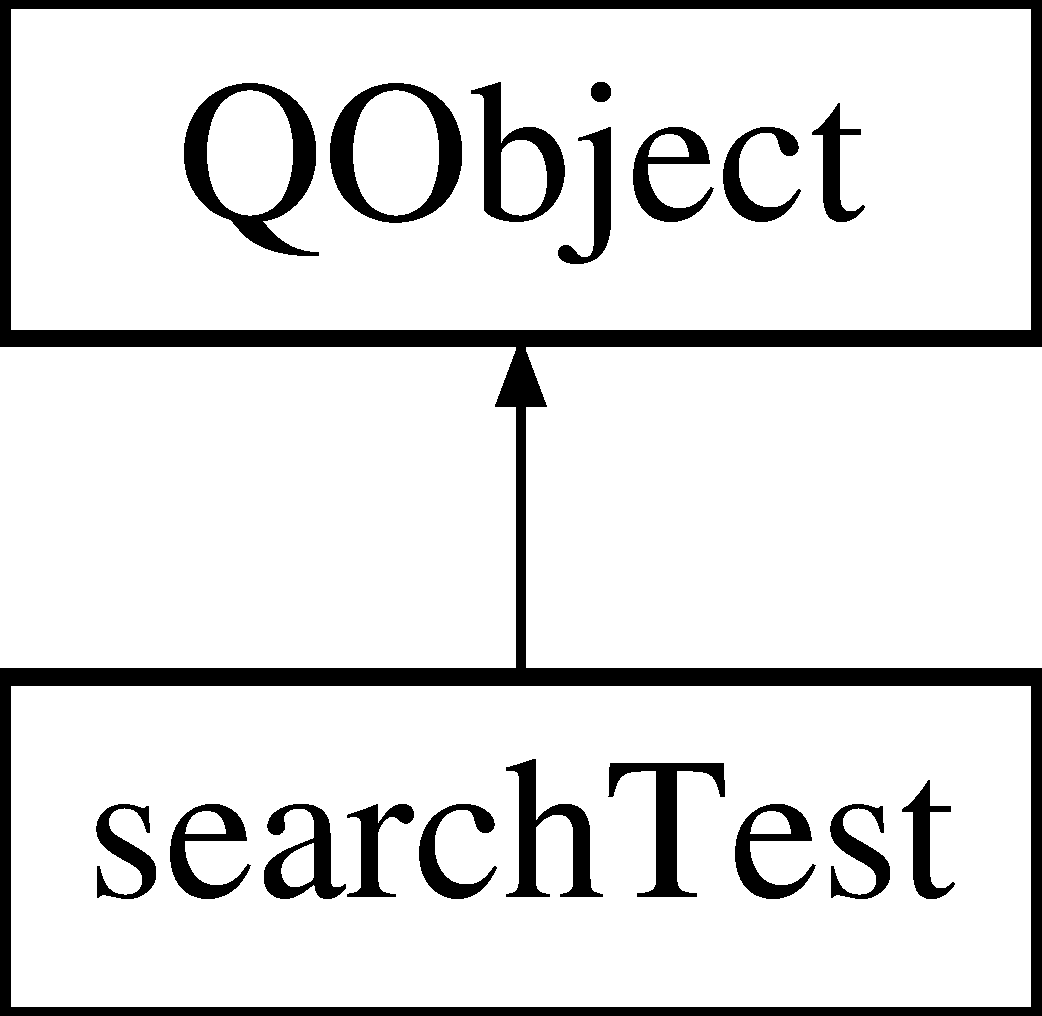
\includegraphics[height=2.000000cm]{d7/d51/classsearchTest}
\end{center}
\end{figure}


The documentation for this class was generated from the following files\+:\begin{DoxyCompactItemize}
\item 
tests/models/searchtest.\+h\item 
tests/models/searchtest.\+cpp\end{DoxyCompactItemize}

\hypertarget{classGui_1_1Widgets_1_1searchWidget}{\section{Gui\-:\-:Widgets\-:\-:search\-Widget Class Reference}
\label{classGui_1_1Widgets_1_1searchWidget}\index{Gui\-::\-Widgets\-::search\-Widget@{Gui\-::\-Widgets\-::search\-Widget}}
}


Class for search in database.  




{\ttfamily \#include $<$searchwidget.\-h$>$}

Inheritance diagram for Gui\-:\-:Widgets\-:\-:search\-Widget\-:\begin{figure}[H]
\begin{center}
\leavevmode
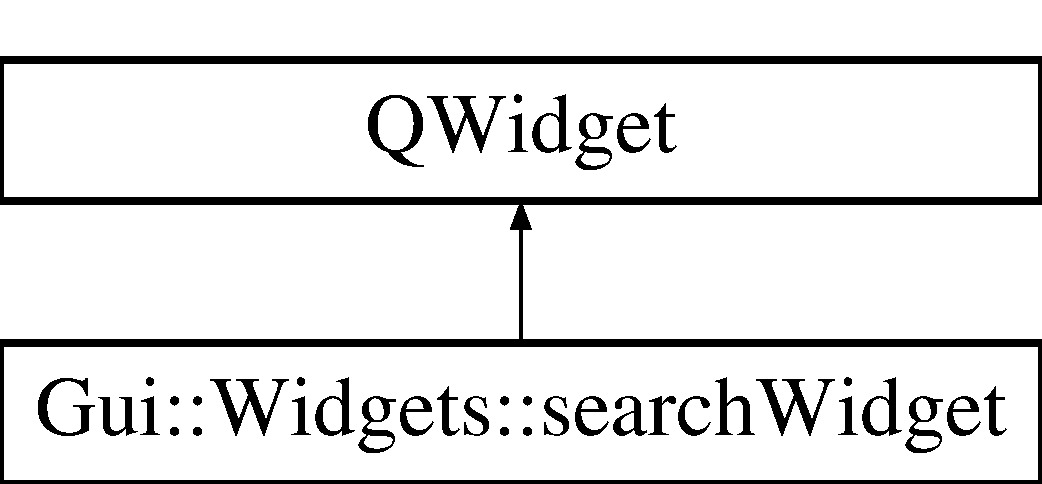
\includegraphics[height=2.000000cm]{d7/d75/classGui_1_1Widgets_1_1searchWidget}
\end{center}
\end{figure}
\subsection*{Public Slots}
\begin{DoxyCompactItemize}
\item 
void \hyperlink{classGui_1_1Widgets_1_1searchWidget_adf91225827fde587bea0d0fc803b0034}{search} (Q\-String to\-Search)
\begin{DoxyCompactList}\small\item\em search\-Widget\-::launch a search \end{DoxyCompactList}\item 
\hypertarget{classGui_1_1Widgets_1_1searchWidget_ae9e5a460a5320c8bfad4d6878009ccbc}{void \hyperlink{classGui_1_1Widgets_1_1searchWidget_ae9e5a460a5320c8bfad4d6878009ccbc}{get\-Customer\-Data} ()}\label{classGui_1_1Widgets_1_1searchWidget_ae9e5a460a5320c8bfad4d6878009ccbc}

\begin{DoxyCompactList}\small\item\em \hyperlink{classGui_1_1Widgets_1_1searchWidget_ae9e5a460a5320c8bfad4d6878009ccbc}{search\-Widget\-::get\-Customer\-Data} Return data on the customer selected in the Q\-Table\-View and display this data (Firstname, Lastname, Company) \end{DoxyCompactList}\end{DoxyCompactItemize}
\subsection*{Signals}
\begin{DoxyCompactItemize}
\item 
\hypertarget{classGui_1_1Widgets_1_1searchWidget_a9b6248c515bac4b6f58237c2f73d804b}{void {\bfseries select\-Customer} ()}\label{classGui_1_1Widgets_1_1searchWidget_a9b6248c515bac4b6f58237c2f73d804b}

\end{DoxyCompactItemize}
\subsection*{Public Member Functions}
\begin{DoxyCompactItemize}
\item 
\hyperlink{classGui_1_1Widgets_1_1searchWidget_a8d77bcf326543f841d1c05fe9819183f}{search\-Widget} (Q\-Widget $\ast$parent=0)
\begin{DoxyCompactList}\small\item\em \hyperlink{classGui_1_1Widgets_1_1searchWidget_a8d77bcf326543f841d1c05fe9819183f}{search\-Widget\-::search\-Widget} Construct a search widget \end{DoxyCompactList}\item 
int \hyperlink{classGui_1_1Widgets_1_1searchWidget_a93c6519cc7e0d8f440451d14fb85bd31}{get\-Current\-Customer\-Id} ()
\begin{DoxyCompactList}\small\item\em \hyperlink{classGui_1_1Widgets_1_1searchWidget_a93c6519cc7e0d8f440451d14fb85bd31}{search\-Widget\-::get\-Current\-Customer\-Id} Return the id of the customer selected in the table \end{DoxyCompactList}\item 
bool \hyperlink{classGui_1_1Widgets_1_1searchWidget_a3cb27e088874c5b8c548d0346a5d85f2}{is\-Customer\-Selected} () const 
\begin{DoxyCompactList}\small\item\em is\-Customer\-Selected Return T\-R\-U\-E if a customer is selected, else F\-A\-L\-S\-E \end{DoxyCompactList}\item 
\hypertarget{classGui_1_1Widgets_1_1searchWidget_a96ba18927785257377dcd3701d41e8d1}{void {\bfseries select\-Customer} (int id)}\label{classGui_1_1Widgets_1_1searchWidget_a96ba18927785257377dcd3701d41e8d1}

\end{DoxyCompactItemize}


\subsection{Detailed Description}
Class for search in database. 

\begin{DoxyAuthor}{Author}
Antoine de Roquemaurel 
\end{DoxyAuthor}


\subsection{Constructor \& Destructor Documentation}
\hypertarget{classGui_1_1Widgets_1_1searchWidget_a8d77bcf326543f841d1c05fe9819183f}{\index{Gui\-::\-Widgets\-::search\-Widget@{Gui\-::\-Widgets\-::search\-Widget}!search\-Widget@{search\-Widget}}
\index{search\-Widget@{search\-Widget}!Gui::Widgets::searchWidget@{Gui\-::\-Widgets\-::search\-Widget}}
\subsubsection[{search\-Widget}]{\setlength{\rightskip}{0pt plus 5cm}Gui\-::\-Widgets\-::search\-Widget\-::search\-Widget (
\begin{DoxyParamCaption}
\item[{Q\-Widget $\ast$}]{parent = {\ttfamily 0}}
\end{DoxyParamCaption}
)\hspace{0.3cm}{\ttfamily [explicit]}}}\label{classGui_1_1Widgets_1_1searchWidget_a8d77bcf326543f841d1c05fe9819183f}


\hyperlink{classGui_1_1Widgets_1_1searchWidget_a8d77bcf326543f841d1c05fe9819183f}{search\-Widget\-::search\-Widget} Construct a search widget 


\begin{DoxyParams}{Parameters}
{\em parent} & The Q\-Widget parent \\
\hline
\end{DoxyParams}


\subsection{Member Function Documentation}
\hypertarget{classGui_1_1Widgets_1_1searchWidget_a93c6519cc7e0d8f440451d14fb85bd31}{\index{Gui\-::\-Widgets\-::search\-Widget@{Gui\-::\-Widgets\-::search\-Widget}!get\-Current\-Customer\-Id@{get\-Current\-Customer\-Id}}
\index{get\-Current\-Customer\-Id@{get\-Current\-Customer\-Id}!Gui::Widgets::searchWidget@{Gui\-::\-Widgets\-::search\-Widget}}
\subsubsection[{get\-Current\-Customer\-Id}]{\setlength{\rightskip}{0pt plus 5cm}int Gui\-::\-Widgets\-::search\-Widget\-::get\-Current\-Customer\-Id (
\begin{DoxyParamCaption}
{}
\end{DoxyParamCaption}
)}}\label{classGui_1_1Widgets_1_1searchWidget_a93c6519cc7e0d8f440451d14fb85bd31}


\hyperlink{classGui_1_1Widgets_1_1searchWidget_a93c6519cc7e0d8f440451d14fb85bd31}{search\-Widget\-::get\-Current\-Customer\-Id} Return the id of the customer selected in the table 

\begin{DoxyReturn}{Returns}
id of the current customer 
\end{DoxyReturn}
\hypertarget{classGui_1_1Widgets_1_1searchWidget_a3cb27e088874c5b8c548d0346a5d85f2}{\index{Gui\-::\-Widgets\-::search\-Widget@{Gui\-::\-Widgets\-::search\-Widget}!is\-Customer\-Selected@{is\-Customer\-Selected}}
\index{is\-Customer\-Selected@{is\-Customer\-Selected}!Gui::Widgets::searchWidget@{Gui\-::\-Widgets\-::search\-Widget}}
\subsubsection[{is\-Customer\-Selected}]{\setlength{\rightskip}{0pt plus 5cm}bool Gui\-::\-Widgets\-::search\-Widget\-::is\-Customer\-Selected (
\begin{DoxyParamCaption}
{}
\end{DoxyParamCaption}
) const}}\label{classGui_1_1Widgets_1_1searchWidget_a3cb27e088874c5b8c548d0346a5d85f2}


is\-Customer\-Selected Return T\-R\-U\-E if a customer is selected, else F\-A\-L\-S\-E 

\begin{DoxyReturn}{Returns}
boolean 
\end{DoxyReturn}
\hypertarget{classGui_1_1Widgets_1_1searchWidget_adf91225827fde587bea0d0fc803b0034}{\index{Gui\-::\-Widgets\-::search\-Widget@{Gui\-::\-Widgets\-::search\-Widget}!search@{search}}
\index{search@{search}!Gui::Widgets::searchWidget@{Gui\-::\-Widgets\-::search\-Widget}}
\subsubsection[{search}]{\setlength{\rightskip}{0pt plus 5cm}void Gui\-::\-Widgets\-::search\-Widget\-::search (
\begin{DoxyParamCaption}
\item[{Q\-String}]{to\-Search}
\end{DoxyParamCaption}
)\hspace{0.3cm}{\ttfamily [slot]}}}\label{classGui_1_1Widgets_1_1searchWidget_adf91225827fde587bea0d0fc803b0034}


search\-Widget\-::launch a search 


\begin{DoxyParams}{Parameters}
{\em to\-Search} & The value to search \\
\hline
\end{DoxyParams}


The documentation for this class was generated from the following files\-:\begin{DoxyCompactItemize}
\item 
/home/florent/\-Documents/\-Projet\-\_\-\-S8/\-Fact\-Dev/src/gui/widgets/searchwidget.\-h\item 
/home/florent/\-Documents/\-Projet\-\_\-\-S8/\-Fact\-Dev/src/gui/widgets/searchwidget.\-cpp\end{DoxyCompactItemize}

\hypertarget{classUtils_1_1String}{\section{Utils\-:\-:String Class Reference}
\label{classUtils_1_1String}\index{Utils\-::\-String@{Utils\-::\-String}}
}


The Utils class.  




{\ttfamily \#include $<$string.\-h$>$}

\subsection*{Static Public Member Functions}
\begin{DoxyCompactItemize}
\item 
static Q\-String \hyperlink{classUtils_1_1String_a9ccf44a6e09a1391001304570ba615a3}{first\-Letter\-To\-Upper} (Q\-String s)
\begin{DoxyCompactList}\small\item\em first\-Letter\-To\-Upper Put the first letter of a string in capslock \end{DoxyCompactList}\end{DoxyCompactItemize}


\subsection{Detailed Description}
The Utils class. 

\begin{DoxyAuthor}{Author}
Antoine de Roquemaurel 
\end{DoxyAuthor}


\subsection{Member Function Documentation}
\hypertarget{classUtils_1_1String_a9ccf44a6e09a1391001304570ba615a3}{\index{Utils\-::\-String@{Utils\-::\-String}!first\-Letter\-To\-Upper@{first\-Letter\-To\-Upper}}
\index{first\-Letter\-To\-Upper@{first\-Letter\-To\-Upper}!Utils::String@{Utils\-::\-String}}
\subsubsection[{first\-Letter\-To\-Upper}]{\setlength{\rightskip}{0pt plus 5cm}Q\-String Utils\-::\-String\-::first\-Letter\-To\-Upper (
\begin{DoxyParamCaption}
\item[{Q\-String}]{s}
\end{DoxyParamCaption}
)\hspace{0.3cm}{\ttfamily [static]}}}\label{classUtils_1_1String_a9ccf44a6e09a1391001304570ba615a3}


first\-Letter\-To\-Upper Put the first letter of a string in capslock 


\begin{DoxyParams}{Parameters}
{\em s} & The string to display \\
\hline
\end{DoxyParams}
\begin{DoxyReturn}{Returns}
The new string with caps 
\end{DoxyReturn}


The documentation for this class was generated from the following files\-:\begin{DoxyCompactItemize}
\item 
/home/travis/build/\-F\-A\-C\-T-\/\-Team/\-Fact\-Dev/src/utils/string.\-h\item 
/home/travis/build/\-F\-A\-C\-T-\/\-Team/\-Fact\-Dev/src/utils/string.\-cpp\end{DoxyCompactItemize}

\hypertarget{classtestadder}{\section{testadder Class Reference}
\label{classtestadder}\index{testadder@{testadder}}
}


The documentation for this class was generated from the following file\-:\begin{DoxyCompactItemize}
\item 
/home/florent/\-Documents/\-Projet\-\_\-\-S8/\-Fact\-Dev/tests/\-Q\-Test\-Runner/testadder.\-h\end{DoxyCompactItemize}

\hypertarget{classTestAdder}{\section{Test\+Adder$<$ T $>$ Class Template Reference}
\label{classTestAdder}\index{Test\+Adder$<$ T $>$@{Test\+Adder$<$ T $>$}}
}
\subsection*{Public Member Functions}
\begin{DoxyCompactItemize}
\item 
\hypertarget{classTestAdder_a64f9008ae27868e36acdd5c94eebae3b}{{\bfseries Test\+Adder} (const Q\+String \&name)}\label{classTestAdder_a64f9008ae27868e36acdd5c94eebae3b}

\end{DoxyCompactItemize}


The documentation for this class was generated from the following file\+:\begin{DoxyCompactItemize}
\item 
tests/\+Q\+Test\+Runner/testadder.\+cpp\end{DoxyCompactItemize}

\hypertarget{classTestRunner}{\section{Test\-Runner Class Reference}
\label{classTestRunner}\index{Test\-Runner@{Test\-Runner}}
}
\subsection*{Public Member Functions}
\begin{DoxyCompactItemize}
\item 
\hypertarget{classTestRunner_affb5703febccf285914b08ce39e7396f}{{\footnotesize template$<$typename T $>$ }\\char {\bfseries Register\-Test} (Q\-String name)}\label{classTestRunner_affb5703febccf285914b08ce39e7396f}

\item 
\hypertarget{classTestRunner_a10db57abd545dd4f9b93e7aeaae55e4c}{int {\bfseries Run\-All} ()}\label{classTestRunner_a10db57abd545dd4f9b93e7aeaae55e4c}

\end{DoxyCompactItemize}
\subsection*{Static Public Member Functions}
\begin{DoxyCompactItemize}
\item 
\hypertarget{classTestRunner_a4707c4680c85ce622fc375efcf39fc25}{static \hyperlink{classTestRunner}{Test\-Runner} \& {\bfseries Instance} ()}\label{classTestRunner_a4707c4680c85ce622fc375efcf39fc25}

\end{DoxyCompactItemize}


The documentation for this class was generated from the following files\-:\begin{DoxyCompactItemize}
\item 
/home/travis/build/\-F\-A\-C\-T-\/\-Team/\-Fact\-Dev/tests/\-Q\-Test\-Runner/testrunner.\-h\item 
/home/travis/build/\-F\-A\-C\-T-\/\-Team/\-Fact\-Dev/tests/\-Q\-Test\-Runner/testrunner.\-cpp\end{DoxyCompactItemize}

\hypertarget{classModels_1_1User}{\section{Models\-:\-:User Class Reference}
\label{classModels_1_1User}\index{Models\-::\-User@{Models\-::\-User}}
}


The \hyperlink{classModels_1_1User}{User} class {\bfseries \hyperlink{classModels_1_1User}{User}} of it application.  




{\ttfamily \#include $<$user.\-h$>$}

Inheritance diagram for Models\-:\-:User\-:\begin{figure}[H]
\begin{center}
\leavevmode
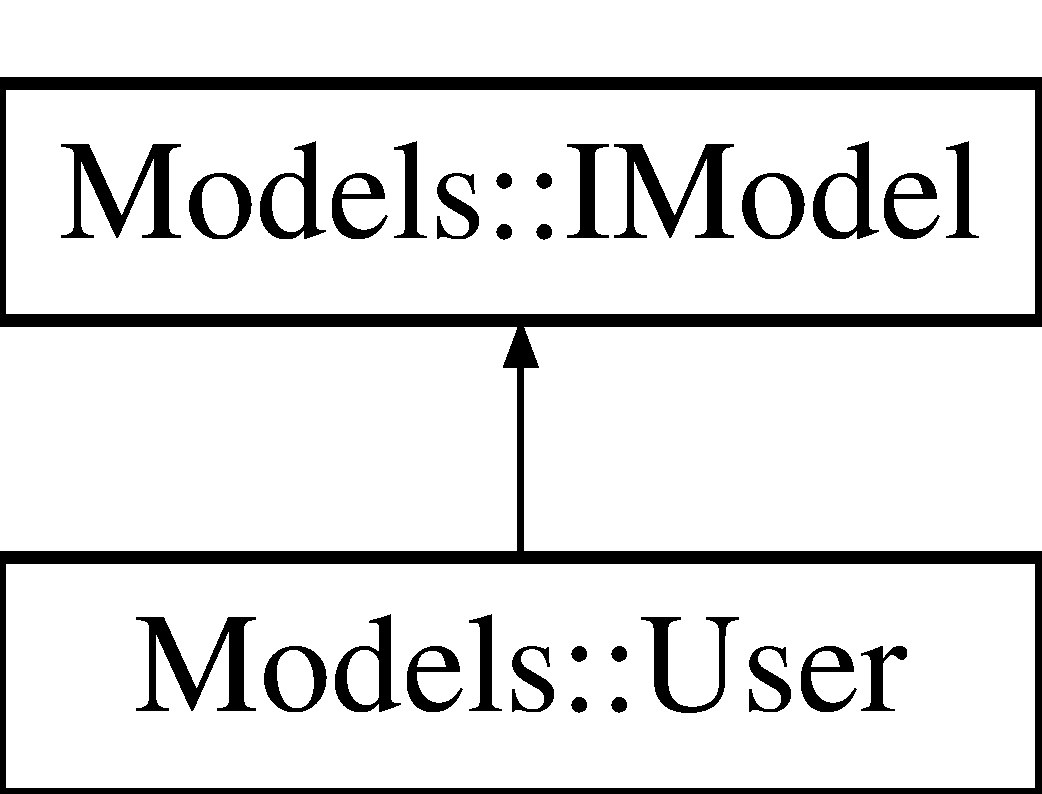
\includegraphics[height=2.000000cm]{df/d68/classModels_1_1User}
\end{center}
\end{figure}
\subsection*{Public Member Functions}
\begin{DoxyCompactItemize}
\item 
\hypertarget{classModels_1_1User_ab106b51be814f7d3a055874781f1f2ee}{\hyperlink{classModels_1_1User_ab106b51be814f7d3a055874781f1f2ee}{User} ()}\label{classModels_1_1User_ab106b51be814f7d3a055874781f1f2ee}

\begin{DoxyCompactList}\small\item\em \hyperlink{classModels_1_1User_ab106b51be814f7d3a055874781f1f2ee}{User\-::\-User}. Contruct an \hyperlink{classModels_1_1User}{User}. \end{DoxyCompactList}\item 
\hyperlink{classModels_1_1User_a8eb50ce05c34b28cf39ff980066f3113}{User} (int id)
\begin{DoxyCompactList}\small\item\em \hyperlink{classModels_1_1User_ab106b51be814f7d3a055874781f1f2ee}{User\-::\-User}. Construct a \hyperlink{classModels_1_1User}{User} with the identify {\itshape id} \end{DoxyCompactList}\item 
\hypertarget{classModels_1_1User_ada0daaa6886be3716af6e15d28c01915}{void \hyperlink{classModels_1_1User_ada0daaa6886be3716af6e15d28c01915}{commit} ()}\label{classModels_1_1User_ada0daaa6886be3716af6e15d28c01915}

\begin{DoxyCompactList}\small\item\em \hyperlink{classModels_1_1User_ada0daaa6886be3716af6e15d28c01915}{User\-::commit} Update user data in \hyperlink{classModels_1_1User}{User} table on the database. \end{DoxyCompactList}\item 
void \hyperlink{classModels_1_1User_ab46c7e1841dca66bc01cd95328b97877}{hydrat} (int id=1)
\begin{DoxyCompactList}\small\item\em \hyperlink{classModels_1_1User_ab46c7e1841dca66bc01cd95328b97877}{User\-::hydrat} Get data of the user who is specified by {\itshape id} from the database. \end{DoxyCompactList}\item 
\hypertarget{classModels_1_1User_ae0870269116b5bda3b5f1c8527e300be}{void \hyperlink{classModels_1_1User_ae0870269116b5bda3b5f1c8527e300be}{remove} ()}\label{classModels_1_1User_ae0870269116b5bda3b5f1c8527e300be}

\begin{DoxyCompactList}\small\item\em remove Remove the current \hyperlink{classModels_1_1User}{User} \end{DoxyCompactList}\item 
Q\-Variant\-Hash \hyperlink{classModels_1_1User_abbc8a3a40b527497872240bf39f21314}{get\-Data\-Map} ()
\begin{DoxyCompactList}\small\item\em get\-Data\-Map Get all data of model with a Hash\-Map key/value \end{DoxyCompactList}\item 
void \hyperlink{classModels_1_1User_ae61c862ac430d25b538601f343f7bf98}{update\-Folders} (void)
\begin{DoxyCompactList}\small\item\em Main\-Window\-::update\-Folders Make directories which contain quotes and billings. Directories are the same than theirs of the Tree organisation (without Projects). \end{DoxyCompactList}\item 
Q\-String \hyperlink{classModels_1_1User_a56a37a1b1125c28e8e72c9a3551b7da5}{get\-Title} () const 
\begin{DoxyCompactList}\small\item\em \hyperlink{classModels_1_1User_a56a37a1b1125c28e8e72c9a3551b7da5}{User\-::get\-Title} Return a short description of \hyperlink{classModels_1_1User}{User} (company) activity. \end{DoxyCompactList}\item 
void \hyperlink{classModels_1_1User_a0fe65ebdee17c2986c874e480e1cb0bd}{set\-Title} (const Q\-String \&title)
\begin{DoxyCompactList}\small\item\em \hyperlink{classModels_1_1User_a0fe65ebdee17c2986c874e480e1cb0bd}{User\-::set\-Title} Modify the user/company activities {\itshape description} \end{DoxyCompactList}\item 
Q\-String \hyperlink{classModels_1_1User_a617ee9ede3791842fbf8593f08660d37}{get\-No\-Siret} () const 
\begin{DoxyCompactList}\small\item\em \hyperlink{classModels_1_1User_a617ee9ede3791842fbf8593f08660d37}{User\-::get\-No\-Siret} Return the S\-I\-R\-E\-T number (company registration number) \end{DoxyCompactList}\item 
void \hyperlink{classModels_1_1User_ae751ee06859dffce0cad08005c42c933}{set\-No\-Siret} (const Q\-String \&no\-Siret)
\begin{DoxyCompactList}\small\item\em \hyperlink{classModels_1_1User_ae751ee06859dffce0cad08005c42c933}{User\-::set\-No\-Siret} Modify the S\-I\-R\-E\-T number (company registration number) {\itshape no\-Siret} \end{DoxyCompactList}\item 
Q\-String \hyperlink{classModels_1_1User_adf4c52429656a4f44c15d879caee5b10}{get\-Workspace\-Name} () const 
\begin{DoxyCompactList}\small\item\em \hyperlink{classModels_1_1User_adf4c52429656a4f44c15d879caee5b10}{User\-::get\-Workspace\-Name} Return the name of the workspace user. \end{DoxyCompactList}\item 
void \hyperlink{classModels_1_1User_ae51aa34e41159fe7e4541a8cfddc50a3}{set\-Workspace\-Name} (const Q\-String \&workspace\-Name)
\begin{DoxyCompactList}\small\item\em \hyperlink{classModels_1_1User_ae51aa34e41159fe7e4541a8cfddc50a3}{User\-::set\-Workspace\-Name} Change the current workspace name by the new {\itshape workspace\-Name} \end{DoxyCompactList}\item 
Q\-String \hyperlink{classModels_1_1User_aa9421bda240316f9eebd0145f6dc3eda}{get\-Workspace\-Path} () const 
\begin{DoxyCompactList}\small\item\em \hyperlink{classModels_1_1User_aa9421bda240316f9eebd0145f6dc3eda}{User\-::get\-Workspace\-Path} Return the path of the workspace user. \end{DoxyCompactList}\item 
void \hyperlink{classModels_1_1User_ae62b6cc7c6c5f5ab80b9f066b67afc95}{set\-Workspace\-Path} (const Q\-String \&workspace\-Path)
\begin{DoxyCompactList}\small\item\em \hyperlink{classModels_1_1User_ae62b6cc7c6c5f5ab80b9f066b67afc95}{User\-::set\-Workspace\-Path} Change the current workspace path by the new {\itshape workspace\-Path} \end{DoxyCompactList}\item 
bool \hyperlink{classModels_1_1User_a60d18c2d1df053f1abf1215414f0b4b6}{operator==} (const \hyperlink{classModels_1_1User}{User} \&u)
\begin{DoxyCompactList}\small\item\em \hyperlink{classModels_1_1User_a60d18c2d1df053f1abf1215414f0b4b6}{User\-::operator ==} Re-\/define the operator \char`\"{}==\char`\"{} to compare if the current \hyperlink{classModels_1_1User}{User} is the same to the other {\bfseries \hyperlink{classModels_1_1User}{User}} {\itshape c} Return T\-R\-U\-E if both Users are the same, else F\-A\-L\-S\-E. \end{DoxyCompactList}\item 
bool \hyperlink{classModels_1_1User_aa1cdb1f752173aedd5f0c43edcb0b10b}{operator!=} (const \hyperlink{classModels_1_1User}{User} \&u)
\begin{DoxyCompactList}\small\item\em \hyperlink{classModels_1_1User_a60d18c2d1df053f1abf1215414f0b4b6}{User\-::operator ==} Re-\/define the operator \char`\"{}!=\char`\"{} to compare if the current \hyperlink{classModels_1_1User}{User} is differnt to the other {\bfseries \hyperlink{classModels_1_1User}{User}} {\itshape c} Return T\-R\-U\-E if both Users are different, else F\-A\-L\-S\-E. \end{DoxyCompactList}\item 
\hypertarget{classModels_1_1User_ae8a894050c3e9266518707f6e5cd1c2f}{Q\-String {\bfseries get\-Pdflatex\-Path} () const }\label{classModels_1_1User_ae8a894050c3e9266518707f6e5cd1c2f}

\item 
\hypertarget{classModels_1_1User_ac65a44513c34f7e67888062d8bee3e54}{void {\bfseries set\-Pdflatex\-Path} (const Q\-String \&get\-Pdflatex\-Path)}\label{classModels_1_1User_ac65a44513c34f7e67888062d8bee3e54}

\end{DoxyCompactItemize}
\subsection*{Additional Inherited Members}


\subsection{Detailed Description}
The \hyperlink{classModels_1_1User}{User} class {\bfseries \hyperlink{classModels_1_1User}{User}} of it application. 

\begin{DoxyAuthor}{Author}
Florent Berbie 
\end{DoxyAuthor}


\subsection{Constructor \& Destructor Documentation}
\hypertarget{classModels_1_1User_a8eb50ce05c34b28cf39ff980066f3113}{\index{Models\-::\-User@{Models\-::\-User}!User@{User}}
\index{User@{User}!Models::User@{Models\-::\-User}}
\subsubsection[{User}]{\setlength{\rightskip}{0pt plus 5cm}Models\-::\-User\-::\-User (
\begin{DoxyParamCaption}
\item[{int}]{id}
\end{DoxyParamCaption}
)}}\label{classModels_1_1User_a8eb50ce05c34b28cf39ff980066f3113}


\hyperlink{classModels_1_1User_ab106b51be814f7d3a055874781f1f2ee}{User\-::\-User}. Construct a \hyperlink{classModels_1_1User}{User} with the identify {\itshape id} 


\begin{DoxyParams}{Parameters}
{\em id} & \hyperlink{classModels_1_1User}{User} id \\
\hline
\end{DoxyParams}


\subsection{Member Function Documentation}
\hypertarget{classModels_1_1User_abbc8a3a40b527497872240bf39f21314}{\index{Models\-::\-User@{Models\-::\-User}!get\-Data\-Map@{get\-Data\-Map}}
\index{get\-Data\-Map@{get\-Data\-Map}!Models::User@{Models\-::\-User}}
\subsubsection[{get\-Data\-Map}]{\setlength{\rightskip}{0pt plus 5cm}Q\-Variant\-Hash Models\-::\-User\-::get\-Data\-Map (
\begin{DoxyParamCaption}
{}
\end{DoxyParamCaption}
)\hspace{0.3cm}{\ttfamily [virtual]}}}\label{classModels_1_1User_abbc8a3a40b527497872240bf39f21314}


get\-Data\-Map Get all data of model with a Hash\-Map key/value 

\begin{DoxyReturn}{Returns}
Model's data 
\end{DoxyReturn}


Implements \hyperlink{classModels_1_1IModel_a9851b0f296aac58353edff22af11cf3c}{Models\-::\-I\-Model}.

\hypertarget{classModels_1_1User_a617ee9ede3791842fbf8593f08660d37}{\index{Models\-::\-User@{Models\-::\-User}!get\-No\-Siret@{get\-No\-Siret}}
\index{get\-No\-Siret@{get\-No\-Siret}!Models::User@{Models\-::\-User}}
\subsubsection[{get\-No\-Siret}]{\setlength{\rightskip}{0pt plus 5cm}Q\-String Models\-::\-User\-::get\-No\-Siret (
\begin{DoxyParamCaption}
{}
\end{DoxyParamCaption}
) const}}\label{classModels_1_1User_a617ee9ede3791842fbf8593f08660d37}


\hyperlink{classModels_1_1User_a617ee9ede3791842fbf8593f08660d37}{User\-::get\-No\-Siret} Return the S\-I\-R\-E\-T number (company registration number) 

\begin{DoxyReturn}{Returns}
S\-I\-R\-E\-T number 
\end{DoxyReturn}
\hypertarget{classModels_1_1User_a56a37a1b1125c28e8e72c9a3551b7da5}{\index{Models\-::\-User@{Models\-::\-User}!get\-Title@{get\-Title}}
\index{get\-Title@{get\-Title}!Models::User@{Models\-::\-User}}
\subsubsection[{get\-Title}]{\setlength{\rightskip}{0pt plus 5cm}Q\-String Models\-::\-User\-::get\-Title (
\begin{DoxyParamCaption}
{}
\end{DoxyParamCaption}
) const}}\label{classModels_1_1User_a56a37a1b1125c28e8e72c9a3551b7da5}


\hyperlink{classModels_1_1User_a56a37a1b1125c28e8e72c9a3551b7da5}{User\-::get\-Title} Return a short description of \hyperlink{classModels_1_1User}{User} (company) activity. 

\begin{DoxyReturn}{Returns}
a short description of user (company) activity 
\end{DoxyReturn}
\hypertarget{classModels_1_1User_adf4c52429656a4f44c15d879caee5b10}{\index{Models\-::\-User@{Models\-::\-User}!get\-Workspace\-Name@{get\-Workspace\-Name}}
\index{get\-Workspace\-Name@{get\-Workspace\-Name}!Models::User@{Models\-::\-User}}
\subsubsection[{get\-Workspace\-Name}]{\setlength{\rightskip}{0pt plus 5cm}Q\-String Models\-::\-User\-::get\-Workspace\-Name (
\begin{DoxyParamCaption}
{}
\end{DoxyParamCaption}
) const}}\label{classModels_1_1User_adf4c52429656a4f44c15d879caee5b10}


\hyperlink{classModels_1_1User_adf4c52429656a4f44c15d879caee5b10}{User\-::get\-Workspace\-Name} Return the name of the workspace user. 

\begin{DoxyReturn}{Returns}
workspace name 
\end{DoxyReturn}
\hypertarget{classModels_1_1User_aa9421bda240316f9eebd0145f6dc3eda}{\index{Models\-::\-User@{Models\-::\-User}!get\-Workspace\-Path@{get\-Workspace\-Path}}
\index{get\-Workspace\-Path@{get\-Workspace\-Path}!Models::User@{Models\-::\-User}}
\subsubsection[{get\-Workspace\-Path}]{\setlength{\rightskip}{0pt plus 5cm}Q\-String Models\-::\-User\-::get\-Workspace\-Path (
\begin{DoxyParamCaption}
{}
\end{DoxyParamCaption}
) const}}\label{classModels_1_1User_aa9421bda240316f9eebd0145f6dc3eda}


\hyperlink{classModels_1_1User_aa9421bda240316f9eebd0145f6dc3eda}{User\-::get\-Workspace\-Path} Return the path of the workspace user. 

\begin{DoxyReturn}{Returns}
workspace path 
\end{DoxyReturn}
\hypertarget{classModels_1_1User_ab46c7e1841dca66bc01cd95328b97877}{\index{Models\-::\-User@{Models\-::\-User}!hydrat@{hydrat}}
\index{hydrat@{hydrat}!Models::User@{Models\-::\-User}}
\subsubsection[{hydrat}]{\setlength{\rightskip}{0pt plus 5cm}void Models\-::\-User\-::hydrat (
\begin{DoxyParamCaption}
\item[{int}]{id = {\ttfamily 1}}
\end{DoxyParamCaption}
)\hspace{0.3cm}{\ttfamily [virtual]}}}\label{classModels_1_1User_ab46c7e1841dca66bc01cd95328b97877}


\hyperlink{classModels_1_1User_ab46c7e1841dca66bc01cd95328b97877}{User\-::hydrat} Get data of the user who is specified by {\itshape id} from the database. 


\begin{DoxyParams}{Parameters}
{\em id} & \hyperlink{classModels_1_1User}{User} identify \\
\hline
\end{DoxyParams}


Implements \hyperlink{classModels_1_1IModel_a7ce6def437f5e1f6a78ee1d67ca028e4}{Models\-::\-I\-Model}.

\hypertarget{classModels_1_1User_aa1cdb1f752173aedd5f0c43edcb0b10b}{\index{Models\-::\-User@{Models\-::\-User}!operator!=@{operator!=}}
\index{operator!=@{operator!=}!Models::User@{Models\-::\-User}}
\subsubsection[{operator!=}]{\setlength{\rightskip}{0pt plus 5cm}bool Models\-::\-User\-::operator!= (
\begin{DoxyParamCaption}
\item[{const {\bf User} \&}]{u}
\end{DoxyParamCaption}
)}}\label{classModels_1_1User_aa1cdb1f752173aedd5f0c43edcb0b10b}


\hyperlink{classModels_1_1User_a60d18c2d1df053f1abf1215414f0b4b6}{User\-::operator ==} Re-\/define the operator \char`\"{}!=\char`\"{} to compare if the current \hyperlink{classModels_1_1User}{User} is differnt to the other {\bfseries \hyperlink{classModels_1_1User}{User}} {\itshape c} Return T\-R\-U\-E if both Users are different, else F\-A\-L\-S\-E. 


\begin{DoxyParams}{Parameters}
{\em u} & \hyperlink{classModels_1_1User}{User} to compare \\
\hline
\end{DoxyParams}
\begin{DoxyReturn}{Returns}
boolean 
\end{DoxyReturn}
\hypertarget{classModels_1_1User_a60d18c2d1df053f1abf1215414f0b4b6}{\index{Models\-::\-User@{Models\-::\-User}!operator==@{operator==}}
\index{operator==@{operator==}!Models::User@{Models\-::\-User}}
\subsubsection[{operator==}]{\setlength{\rightskip}{0pt plus 5cm}bool Models\-::\-User\-::operator== (
\begin{DoxyParamCaption}
\item[{const {\bf User} \&}]{u}
\end{DoxyParamCaption}
)}}\label{classModels_1_1User_a60d18c2d1df053f1abf1215414f0b4b6}


\hyperlink{classModels_1_1User_a60d18c2d1df053f1abf1215414f0b4b6}{User\-::operator ==} Re-\/define the operator \char`\"{}==\char`\"{} to compare if the current \hyperlink{classModels_1_1User}{User} is the same to the other {\bfseries \hyperlink{classModels_1_1User}{User}} {\itshape c} Return T\-R\-U\-E if both Users are the same, else F\-A\-L\-S\-E. 


\begin{DoxyParams}{Parameters}
{\em u} & \hyperlink{classModels_1_1User}{User} to compare \\
\hline
\end{DoxyParams}
\begin{DoxyReturn}{Returns}
boolean 
\end{DoxyReturn}
\hypertarget{classModels_1_1User_ae751ee06859dffce0cad08005c42c933}{\index{Models\-::\-User@{Models\-::\-User}!set\-No\-Siret@{set\-No\-Siret}}
\index{set\-No\-Siret@{set\-No\-Siret}!Models::User@{Models\-::\-User}}
\subsubsection[{set\-No\-Siret}]{\setlength{\rightskip}{0pt plus 5cm}void Models\-::\-User\-::set\-No\-Siret (
\begin{DoxyParamCaption}
\item[{const Q\-String \&}]{no\-Siret}
\end{DoxyParamCaption}
)}}\label{classModels_1_1User_ae751ee06859dffce0cad08005c42c933}


\hyperlink{classModels_1_1User_ae751ee06859dffce0cad08005c42c933}{User\-::set\-No\-Siret} Modify the S\-I\-R\-E\-T number (company registration number) {\itshape no\-Siret} 


\begin{DoxyParams}{Parameters}
{\em no\-Siret} & S\-I\-R\-E\-T number \\
\hline
\end{DoxyParams}
\hypertarget{classModels_1_1User_a0fe65ebdee17c2986c874e480e1cb0bd}{\index{Models\-::\-User@{Models\-::\-User}!set\-Title@{set\-Title}}
\index{set\-Title@{set\-Title}!Models::User@{Models\-::\-User}}
\subsubsection[{set\-Title}]{\setlength{\rightskip}{0pt plus 5cm}void Models\-::\-User\-::set\-Title (
\begin{DoxyParamCaption}
\item[{const Q\-String \&}]{title}
\end{DoxyParamCaption}
)}}\label{classModels_1_1User_a0fe65ebdee17c2986c874e480e1cb0bd}


\hyperlink{classModels_1_1User_a0fe65ebdee17c2986c874e480e1cb0bd}{User\-::set\-Title} Modify the user/company activities {\itshape description} 


\begin{DoxyParams}{Parameters}
{\em title} & Short description on activity(ies) of \hyperlink{classModels_1_1User}{User} company \\
\hline
\end{DoxyParams}
\hypertarget{classModels_1_1User_ae51aa34e41159fe7e4541a8cfddc50a3}{\index{Models\-::\-User@{Models\-::\-User}!set\-Workspace\-Name@{set\-Workspace\-Name}}
\index{set\-Workspace\-Name@{set\-Workspace\-Name}!Models::User@{Models\-::\-User}}
\subsubsection[{set\-Workspace\-Name}]{\setlength{\rightskip}{0pt plus 5cm}void Models\-::\-User\-::set\-Workspace\-Name (
\begin{DoxyParamCaption}
\item[{const Q\-String \&}]{workspace\-Name}
\end{DoxyParamCaption}
)}}\label{classModels_1_1User_ae51aa34e41159fe7e4541a8cfddc50a3}


\hyperlink{classModels_1_1User_ae51aa34e41159fe7e4541a8cfddc50a3}{User\-::set\-Workspace\-Name} Change the current workspace name by the new {\itshape workspace\-Name} 


\begin{DoxyParams}{Parameters}
{\em workspace\-Name} & \\
\hline
\end{DoxyParams}
\hypertarget{classModels_1_1User_ae62b6cc7c6c5f5ab80b9f066b67afc95}{\index{Models\-::\-User@{Models\-::\-User}!set\-Workspace\-Path@{set\-Workspace\-Path}}
\index{set\-Workspace\-Path@{set\-Workspace\-Path}!Models::User@{Models\-::\-User}}
\subsubsection[{set\-Workspace\-Path}]{\setlength{\rightskip}{0pt plus 5cm}void Models\-::\-User\-::set\-Workspace\-Path (
\begin{DoxyParamCaption}
\item[{const Q\-String \&}]{workspace\-Path}
\end{DoxyParamCaption}
)}}\label{classModels_1_1User_ae62b6cc7c6c5f5ab80b9f066b67afc95}


\hyperlink{classModels_1_1User_ae62b6cc7c6c5f5ab80b9f066b67afc95}{User\-::set\-Workspace\-Path} Change the current workspace path by the new {\itshape workspace\-Path} 


\begin{DoxyParams}{Parameters}
{\em workspace\-Path} & \\
\hline
\end{DoxyParams}
\hypertarget{classModels_1_1User_ae61c862ac430d25b538601f343f7bf98}{\index{Models\-::\-User@{Models\-::\-User}!update\-Folders@{update\-Folders}}
\index{update\-Folders@{update\-Folders}!Models::User@{Models\-::\-User}}
\subsubsection[{update\-Folders}]{\setlength{\rightskip}{0pt plus 5cm}void Models\-::\-User\-::update\-Folders (
\begin{DoxyParamCaption}
\item[{void}]{}
\end{DoxyParamCaption}
)}}\label{classModels_1_1User_ae61c862ac430d25b538601f343f7bf98}


Main\-Window\-::update\-Folders Make directories which contain quotes and billings. Directories are the same than theirs of the Tree organisation (without Projects). 

Organisation of folders are formed like this\-:
\begin{DoxyItemize}
\item C\-O\-M\-P\-A\-N\-Y Customer\-Lastname Customer\-Firstname/
\begin{DoxyItemize}
\item Quotes/
\begin{DoxyItemize}
\item quote1 ...
\end{DoxyItemize}
\item Billings/
\begin{DoxyItemize}
\item billing1 ... 
\end{DoxyItemize}
\end{DoxyItemize}
\end{DoxyItemize}

The documentation for this class was generated from the following files\-:\begin{DoxyCompactItemize}
\item 
/home/travis/build/\-F\-A\-C\-T-\/\-Team/\-Fact\-Dev/src/models/user.\-h\item 
/home/travis/build/\-F\-A\-C\-T-\/\-Team/\-Fact\-Dev/src/models/user.\-cpp\end{DoxyCompactItemize}

\hypertarget{classDatabase_1_1UserDatabase}{\section{Database\+:\+:User\+Database Class Reference}
\label{classDatabase_1_1UserDatabase}\index{Database\+::\+User\+Database@{Database\+::\+User\+Database}}
}


The \hyperlink{classDatabase_1_1UserDatabase}{User\+Database} class Access to User data in the the table User of the {\bfseries \hyperlink{classDatabase_1_1Database}{Database}}  




{\ttfamily \#include $<$userdatabase.\+h$>$}

Inheritance diagram for Database\+:\+:User\+Database\+:\begin{figure}[H]
\begin{center}
\leavevmode
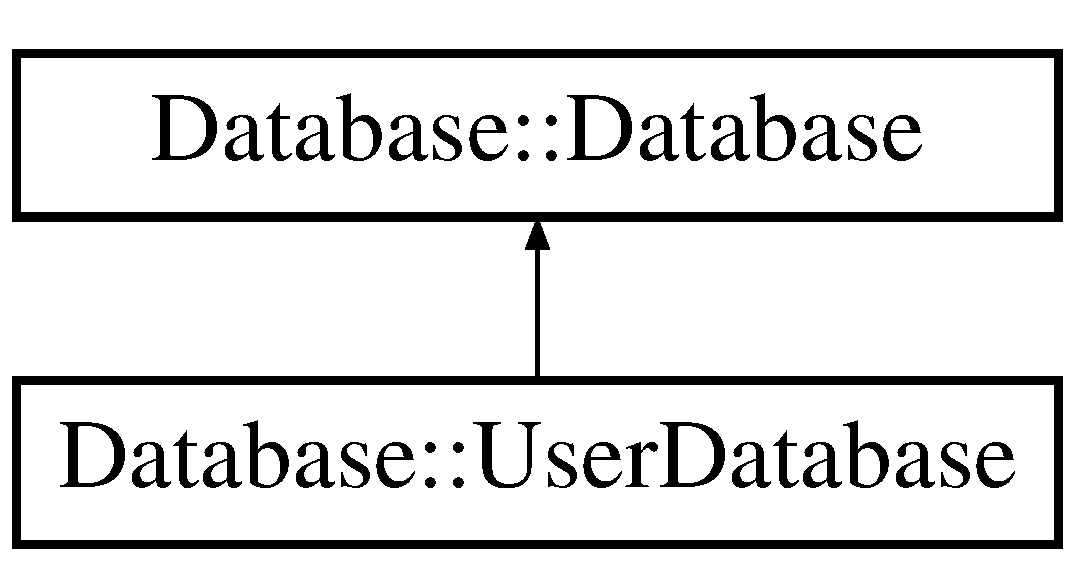
\includegraphics[height=2.000000cm]{d9/d32/classDatabase_1_1UserDatabase}
\end{center}
\end{figure}
\subsection*{Public Member Functions}
\begin{DoxyCompactItemize}
\item 
Q\+Standard\+Item\+Model $\ast$ \hyperlink{classDatabase_1_1UserDatabase_a1b35f88b06fc54521bb72acd1fbbdc1e}{get\+User\+Table} ()  throw (\+Db\+Exception$\ast$)
\begin{DoxyCompactList}\small\item\em get\+User\+Table Return an item model of User for Q\+Table\+View \end{DoxyCompactList}\item 
\hyperlink{classModels_1_1User}{Models\+::\+User} $\ast$ \hyperlink{classDatabase_1_1UserDatabase_ad05795be223fef14a114d712aebef2e6}{get\+User} (const int p\+Id=1)
\begin{DoxyCompactList}\small\item\em get\+User Get informations about the user (identified by 'p\+Id') \end{DoxyCompactList}\item 
\hypertarget{classDatabase_1_1UserDatabase_af00cc95c910ab6ca3dbeef591531ae2b}{void \hyperlink{classDatabase_1_1UserDatabase_af00cc95c910ab6ca3dbeef591531ae2b}{update\+User} (const \hyperlink{classModels_1_1User}{Models\+::\+User} \&)}\label{classDatabase_1_1UserDatabase_af00cc95c910ab6ca3dbeef591531ae2b}

\begin{DoxyCompactList}\small\item\em update\+User Update informations about the user \end{DoxyCompactList}\end{DoxyCompactItemize}
\subsection*{Static Public Member Functions}
\begin{DoxyCompactItemize}
\item 
static \hyperlink{classDatabase_1_1UserDatabase}{User\+Database} $\ast$ \hyperlink{classDatabase_1_1UserDatabase_ac8cdf7dc9b0163d832ca473973916952}{instance} ()  throw (\+Db\+Exception$\ast$)
\begin{DoxyCompactList}\small\item\em User\+Database\+::get\+Instance Return an instance of \hyperlink{classDatabase_1_1UserDatabase}{User\+Database}. \end{DoxyCompactList}\end{DoxyCompactItemize}
\subsection*{Additional Inherited Members}


\subsection{Detailed Description}
The \hyperlink{classDatabase_1_1UserDatabase}{User\+Database} class Access to User data in the the table User of the {\bfseries \hyperlink{classDatabase_1_1Database}{Database}} 

\begin{DoxyAuthor}{Author}
Florent Berbie 
\end{DoxyAuthor}
\begin{DoxySeeAlso}{See also}
\hyperlink{classDatabase_1_1Database}{Database} 

User 
\end{DoxySeeAlso}


\subsection{Member Function Documentation}
\hypertarget{classDatabase_1_1UserDatabase_ad05795be223fef14a114d712aebef2e6}{\index{Database\+::\+User\+Database@{Database\+::\+User\+Database}!get\+User@{get\+User}}
\index{get\+User@{get\+User}!Database\+::\+User\+Database@{Database\+::\+User\+Database}}
\subsubsection[{get\+User}]{\setlength{\rightskip}{0pt plus 5cm}{\bf Models\+::\+User} $\ast$ Database\+::\+User\+Database\+::get\+User (
\begin{DoxyParamCaption}
\item[{const int}]{p\+Id = {\ttfamily 1}}
\end{DoxyParamCaption}
)}}\label{classDatabase_1_1UserDatabase_ad05795be223fef14a114d712aebef2e6}


get\+User Get informations about the user (identified by 'p\+Id') 


\begin{DoxyParams}{Parameters}
{\em p\+Id} & user id (1 default) $\ast$ \\
\hline
\end{DoxyParams}
\begin{DoxyReturn}{Returns}
the user 
\end{DoxyReturn}
\hypertarget{classDatabase_1_1UserDatabase_a1b35f88b06fc54521bb72acd1fbbdc1e}{\index{Database\+::\+User\+Database@{Database\+::\+User\+Database}!get\+User\+Table@{get\+User\+Table}}
\index{get\+User\+Table@{get\+User\+Table}!Database\+::\+User\+Database@{Database\+::\+User\+Database}}
\subsubsection[{get\+User\+Table}]{\setlength{\rightskip}{0pt plus 5cm}Q\+Standard\+Item\+Model$\ast$ Database\+::\+User\+Database\+::get\+User\+Table (
\begin{DoxyParamCaption}
{}
\end{DoxyParamCaption}
) throw  {\bf Db\+Exception} $\ast$) }}\label{classDatabase_1_1UserDatabase_a1b35f88b06fc54521bb72acd1fbbdc1e}


get\+User\+Table Return an item model of User for Q\+Table\+View 

\begin{DoxyReturn}{Returns}
Q\+Standard\+Item\+Model an item model 
\end{DoxyReturn}
\hypertarget{classDatabase_1_1UserDatabase_ac8cdf7dc9b0163d832ca473973916952}{\index{Database\+::\+User\+Database@{Database\+::\+User\+Database}!instance@{instance}}
\index{instance@{instance}!Database\+::\+User\+Database@{Database\+::\+User\+Database}}
\subsubsection[{instance}]{\setlength{\rightskip}{0pt plus 5cm}{\bf User\+Database} $\ast$ Database\+::\+User\+Database\+::instance (
\begin{DoxyParamCaption}
{}
\end{DoxyParamCaption}
) throw  {\bf Db\+Exception} $\ast$) \hspace{0.3cm}{\ttfamily [static]}}}\label{classDatabase_1_1UserDatabase_ac8cdf7dc9b0163d832ca473973916952}


User\+Database\+::get\+Instance Return an instance of \hyperlink{classDatabase_1_1UserDatabase}{User\+Database}. 

\begin{DoxyReturn}{Returns}
Instance of \hyperlink{classDatabase_1_1UserDatabase}{User\+Database} 
\end{DoxyReturn}


The documentation for this class was generated from the following files\+:\begin{DoxyCompactItemize}
\item 
src/database/userdatabase.\+h\item 
src/database/userdatabase.\+cpp\end{DoxyCompactItemize}

\hypertarget{classGui_1_1Dialogs_1_1UserDataDialog}{\section{Gui\-:\-:Dialogs\-:\-:User\-Data\-Dialog Class Reference}
\label{classGui_1_1Dialogs_1_1UserDataDialog}\index{Gui\-::\-Dialogs\-::\-User\-Data\-Dialog@{Gui\-::\-Dialogs\-::\-User\-Data\-Dialog}}
}


The \hyperlink{classGui_1_1Dialogs_1_1UserDataDialog}{User\-Data\-Dialog} class Window to fill user data.  




{\ttfamily \#include $<$userdatadialog.\-h$>$}

Inheritance diagram for Gui\-:\-:Dialogs\-:\-:User\-Data\-Dialog\-:\begin{figure}[H]
\begin{center}
\leavevmode
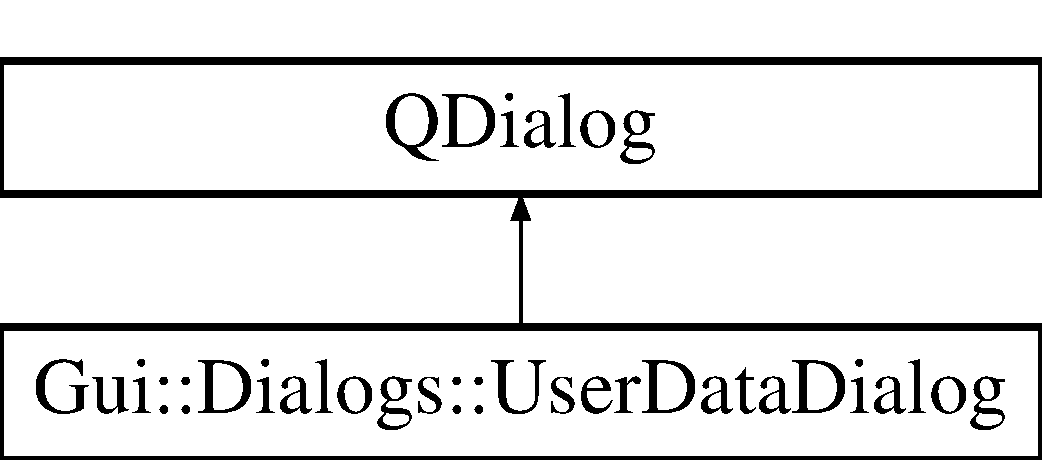
\includegraphics[height=2.000000cm]{d3/d81/classGui_1_1Dialogs_1_1UserDataDialog}
\end{center}
\end{figure}
\subsection*{Public Slots}
\begin{DoxyCompactItemize}
\item 
\hypertarget{classGui_1_1Dialogs_1_1UserDataDialog_a9ab536a7485460c905a8f17be8939f38}{void \hyperlink{classGui_1_1Dialogs_1_1UserDataDialog_a9ab536a7485460c905a8f17be8939f38}{check\-Fields} ()}\label{classGui_1_1Dialogs_1_1UserDataDialog_a9ab536a7485460c905a8f17be8939f38}

\begin{DoxyCompactList}\small\item\em \hyperlink{classGui_1_1Dialogs_1_1UserDataDialog_a9ab536a7485460c905a8f17be8939f38}{User\-Data\-Dialog\-::check\-Fields} Check all fields of dialog components. \end{DoxyCompactList}\item 
\hypertarget{classGui_1_1Dialogs_1_1UserDataDialog_a7516a1eb19fa88dc405c085cefa6a3b6}{void \hyperlink{classGui_1_1Dialogs_1_1UserDataDialog_a7516a1eb19fa88dc405c085cefa6a3b6}{browse\-Workspace\-Path} ()}\label{classGui_1_1Dialogs_1_1UserDataDialog_a7516a1eb19fa88dc405c085cefa6a3b6}

\begin{DoxyCompactList}\small\item\em \hyperlink{classGui_1_1Dialogs_1_1UserDataDialog_a7516a1eb19fa88dc405c085cefa6a3b6}{User\-Data\-Dialog\-::browse\-Workspace\-Path} Open a new window to define the workspace path of the user. \end{DoxyCompactList}\end{DoxyCompactItemize}
\subsection*{Public Member Functions}
\begin{DoxyCompactItemize}
\item 
\hyperlink{classGui_1_1Dialogs_1_1UserDataDialog_a3cafa419d49d124e72511a3b91f8ee76}{User\-Data\-Dialog} (Q\-Widget $\ast$parent=0)
\begin{DoxyCompactList}\small\item\em \hyperlink{classGui_1_1Dialogs_1_1UserDataDialog_a3cafa419d49d124e72511a3b91f8ee76}{User\-Data\-Dialog\-::\-User\-Data\-Dialog} Construct a window with user data. \end{DoxyCompactList}\item 
\hypertarget{classGui_1_1Dialogs_1_1UserDataDialog_ae1a17e6547a30b03ba2c837ba0b28455}{void \hyperlink{classGui_1_1Dialogs_1_1UserDataDialog_ae1a17e6547a30b03ba2c837ba0b28455}{fill\-Fields} ()}\label{classGui_1_1Dialogs_1_1UserDataDialog_ae1a17e6547a30b03ba2c837ba0b28455}

\begin{DoxyCompactList}\small\item\em \hyperlink{classGui_1_1Dialogs_1_1UserDataDialog_ae1a17e6547a30b03ba2c837ba0b28455}{User\-Data\-Dialog\-::fill\-Fields} Fill line edits with the data of the user. \end{DoxyCompactList}\item 
\hypertarget{classGui_1_1Dialogs_1_1UserDataDialog_a2d3841c471d0ddfd58610d3667d8521a}{void \hyperlink{classGui_1_1Dialogs_1_1UserDataDialog_a2d3841c471d0ddfd58610d3667d8521a}{accept} ()}\label{classGui_1_1Dialogs_1_1UserDataDialog_a2d3841c471d0ddfd58610d3667d8521a}

\begin{DoxyCompactList}\small\item\em \hyperlink{classGui_1_1Dialogs_1_1UserDataDialog_a2d3841c471d0ddfd58610d3667d8521a}{User\-Data\-Dialog\-::accept} Valid data inputed by user and add these data in Database. \end{DoxyCompactList}\item 
\hypertarget{classGui_1_1Dialogs_1_1UserDataDialog_a919f59546670019bb4e72fcd0c7ea841}{void \hyperlink{classGui_1_1Dialogs_1_1UserDataDialog_a919f59546670019bb4e72fcd0c7ea841}{reject} ()}\label{classGui_1_1Dialogs_1_1UserDataDialog_a919f59546670019bb4e72fcd0c7ea841}

\begin{DoxyCompactList}\small\item\em \hyperlink{classGui_1_1Dialogs_1_1UserDataDialog_a919f59546670019bb4e72fcd0c7ea841}{User\-Data\-Dialog\-::reject} Cancel the operation and close the windows. \end{DoxyCompactList}\end{DoxyCompactItemize}


\subsection{Detailed Description}
The \hyperlink{classGui_1_1Dialogs_1_1UserDataDialog}{User\-Data\-Dialog} class Window to fill user data. 

\begin{DoxyAuthor}{Author}
Florent Berbie 
\end{DoxyAuthor}
\begin{DoxySeeAlso}{See Also}
Project 
\end{DoxySeeAlso}


\subsection{Constructor \& Destructor Documentation}
\hypertarget{classGui_1_1Dialogs_1_1UserDataDialog_a3cafa419d49d124e72511a3b91f8ee76}{\index{Gui\-::\-Dialogs\-::\-User\-Data\-Dialog@{Gui\-::\-Dialogs\-::\-User\-Data\-Dialog}!User\-Data\-Dialog@{User\-Data\-Dialog}}
\index{User\-Data\-Dialog@{User\-Data\-Dialog}!Gui::Dialogs::UserDataDialog@{Gui\-::\-Dialogs\-::\-User\-Data\-Dialog}}
\subsubsection[{User\-Data\-Dialog}]{\setlength{\rightskip}{0pt plus 5cm}Gui\-::\-Dialogs\-::\-User\-Data\-Dialog\-::\-User\-Data\-Dialog (
\begin{DoxyParamCaption}
\item[{Q\-Widget $\ast$}]{parent = {\ttfamily 0}}
\end{DoxyParamCaption}
)\hspace{0.3cm}{\ttfamily [explicit]}}}\label{classGui_1_1Dialogs_1_1UserDataDialog_a3cafa419d49d124e72511a3b91f8ee76}


\hyperlink{classGui_1_1Dialogs_1_1UserDataDialog_a3cafa419d49d124e72511a3b91f8ee76}{User\-Data\-Dialog\-::\-User\-Data\-Dialog} Construct a window with user data. 


\begin{DoxyParams}{Parameters}
{\em parent} & \\
\hline
\end{DoxyParams}


The documentation for this class was generated from the following files\-:\begin{DoxyCompactItemize}
\item 
/home/travis/build/\-F\-A\-C\-T-\/\-Team/\-Fact\-Dev/src/gui/dialogs/userdatadialog.\-h\item 
/home/travis/build/\-F\-A\-C\-T-\/\-Team/\-Fact\-Dev/src/gui/dialogs/userdatadialog.\-cpp\end{DoxyCompactItemize}

%--- End generated contents ---

% Index
\newpage
\phantomsection
\addcontentsline{toc}{chapter}{Index}
\printindex

\end{document}
